% !Mode:: "TeX:UTF-8"
% !TEX encoding = UTF-8 Unicode

%----------------------------------------------------------------------------------------
% 机器翻译:统计建模与深度学习方法
% Machine Translation: Statistical Modeling and Deep Learning Methods
%
% Copyright 2020
% 肖桐(xiaotong@mail.neu.edu.cn) 朱靖波 (zhujingbo@mail.neu.edu.cn)
%----------------------------------------------------------------------------------------

\part{神经机器翻译}
%----------------------------------------------------------------------------------------
%    CONFIGURATIONS
%----------------------------------------------------------------------------------------

\renewcommand\figurename{图}% Figure => 图
\renewcommand\tablename{表}% Table => 表
\definecolor{ublue}{rgb}{0.152,0.250,0.545} % Color of deep blue
\definecolor{ugreen}{rgb}{0,0.5,0} % Color of deep green
\chapterimage{fig-NEU-6.jpg} % Chapter heading image

%----------------------------------------------------------------------------------------
%    CHAPTER 5
%----------------------------------------------------------------------------------------

\chapter{人工神经网络和神经语言建模}

\parinterval {\small\sffamily\bfseries{人工神经网络}}\index{人工神经网络}(Artificial Neural Networks)\index{Artificial Neural Networks}或{\small\sffamily\bfseries{神经网络}}\index{神经网络}(Neural Networks)\index{Neural Networks}是描述客观世界的一种数学模型。这种模型和生物学上的神经系统在行为上有一些相似之处,但是人们更多的是把它作为一种计算工具,而非一个生物学模型。近些年,随着机器学习领域的快速发展,人工神经网络被更多的使用在对图像和自然语言处理问题的建模上。特别是,研究人员发现深层神经网络可以被成功训练后,学术界也逐渐形成了一种新的机器学习范式\ \dash \ 深度学习。可以说,深度学习是近几年最受瞩目的研究领域之一,其应用也十分广泛。比如,图像识别的很多重要进展都来自深度学习模型的使用。包括机器翻译在内的很多自然语言处理任务中,深度学习也已经成为了一种标准模型。基于深度学习的表示学习方法也为自然语言处理开辟了新的思路。

\parinterval 本章将对深度学习的概念和技术进行介绍,目的是为第六章和第七章神经机器翻译的内容进行铺垫。此外,本章也会对深度学习在语言建模方面的应用进行介绍。这样,读者可以更容易地理解如何使用深度学习方法描述自然语言处理问题。同时,进一步了解一些相关的学术前沿,如预训练模型。\\ \\ \\

%----------------------------------------------------------------------------------------
%    NEW SECTION
%----------------------------------------------------------------------------------------

\section{深度学习与人工神经网络}

\parinterval {\small\sffamily\bfseries{深度学习}}\index{深度学习}(Deep Learning)\index{Deep Learning}是机器学习研究中一个非常重要的分支,其概念来源于对人工神经网络的研究:通过人工神经元之间的连接建立一种数学模型,使计算机可以像人一样进行分析、学习和推理。

\parinterval 近几年来,随着深度学习技术的广泛传播与使用,``人工智能''这个名词在有些场合下甚至与``深度学习''划上了等号。这种理解非常片面,比较准确地说,``深度学习''是实现``人工智能''的一种技术手段。但从这种现象中,深度学习的火爆情况可见一斑。深度学习的技术浪潮以惊人的速度席卷世界,也改变了很多领域的现状,在数据挖掘、自然语言处理、语音识别、图像识别等各个领域随处可见深度学习的身影。自然语言处理领域中,深度学习在很多任务中已经处于``统治''地位。特别是,基于深度学习的表示学习方法已经成为自然语言处理的新范式,在机器翻译任务中更是衍生出了``神经机器翻译''这样全新的模型。

%----------------------------------------------------------------------------------------
%    NEW SUB-SECTION
%----------------------------------------------------------------------------------------

\subsection{发展简史}

\parinterval 神经网络最早出现在控制论中,随后更多地在连接主义中被提及。神经网络被提出的初衷并不是利用神经网络做一个简单的计算模型,而是希望将神经网络应用到一些自动控制相关的场景中。然而随着神经网络技术的持续发展,神经网络方法已经被广泛应用到各行各业的研究和实践工作中。

\parinterval 人工神经网络自1943年诞生至今,经历了多次高潮和低谷,这是任何一种技术都无法绕开的命运。然而,好的技术和方法终究不会被埋没,直到今天,神经网络和深度学习迎来了最好的20年。

%----------------------------------------------------------------------------------------
%    NEW SUBSUB-SECTION
%----------------------------------------------------------------------------------------

\subsubsection{早期的人工神经网络和第一次寒冬}

\parinterval 最初,神经网络设计的初衷是用计算模型来模拟生物大脑中神经元的运行机理,这种想法哪怕是现在看来也是十分超前的。例如,目前很多机构关注的概念\ \dash \ ``类脑计算''就是希望研究人脑的运行机制及相关的计算机实现方法。然而模拟大脑这件事并没有想象中的那么简单,众所周知,生物学中对人脑机制的研究是十分困难的,我们对人脑的运行机制尚不明确又何谈模拟呢?因而,神经网络技术一直在摸索着前行,发展到现在,其计算过程与人脑的运行机制已经大相径庭。

\parinterval 人工神经网络的第一个发展阶段是在二十世纪40年代到70年代,这个时期的人工神经网络还停留在利用线性模型模拟生物神经元的阶段,比如使用线性加权函数来描述输入$ \mathbf x $和输出$ y $ 之间的联系:$y=x_1 \cdot w_1 + \dots + x_n \cdot w_n $。举一个简单例子,输入$ \mathbf x $是某个地区的坐标和时间,输出$ y $是该地区的温度,尽管真实的问题可能要复杂的多,但是线性模型确实有能力去拟合简单的函数关系。

\parinterval 这种线性模型在现在看来可能比较``简陋'',但是这类模型对后来的随机梯度下降等经典方法产生了深远影响。不过,显而易见的是,这种结构也存在着非常明显的缺陷,单层结构限制了它的学习能力,使它无法描述非线性问题,如著名的异或函数(XOR)学习问题,然而非线性才是现实世界的普遍特征,第一代人工神经网络对很多事物的规律都无法准确描述。此后,神经网络的研究陷入了很长一段时间的低迷期。

%----------------------------------------------------------------------------------------
%    NEW SUBSUB-SECTION
%----------------------------------------------------------------------------------------

\subsubsection{神经网络的第二次高潮和第二次寒冬}

\parinterval 虽然第一代神经网络受到了打击,但是20世纪80年代,第二代人工神经网络开始萌发新的生机。在这个发展阶段,生物属性已经不再是神经网络的唯一灵感来源,在{\small\bfnew{连接主义}}\index{连接主义}(Connectionism)\index{Connectionism}和{\small\bfnew{分布式表示}}\index{分布式表示}(Distributed representation)\index{Distributed representation}两种思潮的影响下,神经网络方法再次走入了人们的视线。

\vspace{0.3em}
\parinterval (1)符号主义与连接主义
\vspace{0.3em}

\parinterval 人工智能领域始终存在着符号主义和连接主义之争。早期的人工智能研究在认知学中被称为{\small\bfnew{符号主义}}\index{符号主义}(Symbolicism)\index{Symbolicism},符号主义认为人工智能源于数理逻辑,希望将世界万物的所有运转方式归纳成像文法一样符合逻辑规律的推导过程。符号主义的支持者们坚信基于物理符号系统(即符号操作系统)假设和有限合理性原理,就能通过逻辑推理来模拟智能。但被他们忽略的一点是,模拟智能的推理过程需要大量的先验知识支持,哪怕是在现代,生物学界也很难解释大脑中神经元的工作原理,因此也很难用符号系统刻画人脑逻辑。另一方面,连接主义则侧重于利用人工神经网络中神经元的连接去探索并模拟输入与输出之间存在的某种关系,这个过程不需要任何先验知识,其核心思想是``大量简单的计算单元连接到一起可以实现智能行为'',这种思想也推动了反向传播等多层神经网络方法的应用,并发展了包括长短时记忆模型在内的经典建模方法。2019年3月27日,ACM 正式宣布将图灵奖授予 Yoshua Bengio, Geoffrey Hinton 和 Yann LeCun,以表彰他们提出的概念和工作使得深度学习神经网络有了重大突破,这三位获奖人均是人工智能连接主义学派的主要代表,从这件事中也可以看出连接主义对当代人工智能和深度学习的巨大影响。

\vspace{0.3em}
\parinterval (2)分布式表示
\vspace{0.3em}

\parinterval 分布式表示的主要思想是``一个复杂系统的任何部分的输入都应该是多个特征共同表示的结果'',这种思想在自然语言处理领域的影响尤其深刻,它改变了刻画世界的角度,将世界万物从离散空间映射到多维连续空间。例如,在现实世界中,``张三''这个代号就代表着一个人。如果想要知道这个人亲属都有谁,因为有``A和B如果姓氏相同,在一个家谱中,那么A和B是本家''这个先验知识在,在知道代号``张三''的情况下,可以得知``张三''的亲属是谁。但是如果不依靠这个先验知识,就无法得知``张三''的亲属是谁。但在分布式表示中,可以用一个实数向量,如$ (0.1,0.3,0.4) $来表示``张三''这个人,这个人的所有特征信息都包含在这个实数向量中,通过在向量空间中的一些操作(如计算距离等),哪怕没有任何先验知识的存在,也完全可以找到这个人的所有亲属。在自然语言处理中,一个单词也用一个实数向量(词向量或词嵌入)表示,通过这种方式将语义空间重新刻画,将这个离散空间转化成了一个连续空间,这时单词就不再是一个简单的词条,而是由成百上千个特征共同描述出来的,其中每个特征分别代表这个词的某个`` 方面''。

\parinterval 随着第二代人工神经网络的``脱胎换骨'',学者们又对神经网络方法燃起了希望之火,这也导致有些时候过分夸大了神经网络的能力。20世纪90年代后期,由于在语音识别、自然语言处理等应用中,人们对神经网络方法期望过高,但是结果并没有达到预期,这也让很多人丧失了对神经网络方法的信任。相反,核方法、图模型等机器学习方法取得了很好的效果,这导致神经网络研究又一次进入低谷。

%----------------------------------------------------------------------------------------
%    NEW SUBSUB-SECTION
%----------------------------------------------------------------------------------------

\subsubsection{深度学习和神经网络方法的崛起}

\parinterval 21世纪初,随着深度学习浪潮席卷世界,人工神经网络又一次出现在人们的视野中。深度学习的流行源于2006年Hinton等人成功训练了一个深度信念网络(Deep Belief Network),在深度神经网络方法完全不受重视的情况下,大家突然发现深度神经网络完全是一个魔鬼般的存在,可以解决很多当时其他方法无法解决的问题。神经网络方法终于在一次又一次的被否定后,迎来了它的春天。随之针对神经网络和深度学习的一系列研究前赴后继地展开了,延续至今。

\parinterval 回过头来看,现代深度学习的成功主要有三方面的原因:

\begin{itemize}
\vspace{0.5em}
\item 第一,模型和算法的不断完善和改进。这是现代深度学习能够获得成功的最主要原因;
\vspace{0.5em}
\item 第二,并行计算能力的提升使大规模的实践成为了可能。早期的计算机设备根本无法支撑深度神经网络训练所需要的计算量,导致实践变得十分困难。而设备的进步、计算能力的提升则彻底改变了这种窘境;
\vspace{0.5em}
\item 第三,以Hinton等人为代表的学者的坚持和持续投入。
\vspace{0.5em}
\end{itemize}

\parinterval 另外,从应用的角度,数据量的快速提升和模型容量的增加也为深度学习的成功提供了条件,数据量的增加使得深度学习有了用武之地,例如,2000年以来,双文本数据量无论在学术研究还是在工业实践中的使用数量都在逐年上升(如图\ref{fig:5-1}所示)。现在的深度学习模型参数量往往很大,因此需要大规模数据才能保证模型学习的充分性,而大数据时代的到来为训练这样的模型提供了数据基础。

%----------------------------------------------------------------------
\begin{figure}[htp]
\centering
 %%%------------------------------------------------------------------------------------------------------------
 \begin{tikzpicture}
      \scriptsize{
\begin{semilogyaxis}[
    width=.75\textwidth,
    height=.30\textwidth,
    yticklabel style={/pgf/number format/precision=1,/pgf/number format/fixed zerofill},
    xticklabel style={/pgf/number format/1000 sep=},
    xlabel style={yshift=0.5em},
    xlabel={\footnotesize{Year}},ylabel={\footnotesize{\# of sents.}},
    ymin=1,ymax=1000000000000,
    xmin=1999,xmax=2020,xtick={2000,2005,2010,2015,2020},
    legend style={yshift=-5em,xshift=0em,legend cell align=left,legend plot pos=right}
]

\addplot[purple,mark=square,mark=star,very thick] coordinates {(2001,10000) (2005,2000000) (2008,8000000) (2009,9000000) (2011,10000000) (2012,12000000) (2014,20000000) (2016,30000000) (2018,40000000) };
\addlegendentry{\tiny{Bi-text used in MT papers}\ \ \ \ \ \ \ \ \ \ }
{
\addplot[ublue,mark=otimes*,very thick] coordinates {(2005,10000000) (2008,100000000) (2012,3000000000) (2016,5000000000) (2019,10000000000) };
\addlegendentry{\tiny{Bi-text used in practical systems}}
}

\end{semilogyaxis}
}
 \end{tikzpicture}









%%%------------------------------------------------------------------------------------------------------------

\caption{2000年以来各年的双语数据量}
\label{fig:5-1}
\end{figure}
%----------------------------------------------------------------------

%----------------------------------------------------------------------------------------
%    NEW SUB-SECTION
%----------------------------------------------------------------------------------------

\subsection{为什么需要深度学习}

\parinterval 深度神经网络提供了一种简单的学习机制,即直接学习输入与输出的关系,通常把这种机制称为{\small\bfnew{端到端学习}}\index{端到端学习}(End-to-End Learning)\index{End-to-End Learning}。与传统方法不同,端到端学习并不需要人工定义特征或者进行过多的先验性假设,所有的学习过程都是由一个模型完成。从外面看这个模型只是建立了一种输入到输出的映射,而这种映射具体是如何形成的完全由模型的结构和参数决定。这样做的最大好处是,模型可以更加``自由''的进行学习。此外,端到端学习也引发了一个新的思考\ \dash \ 如何表示问题?这也就是所谓的{\small\bfnew{表示学习}}\index{表示学习}(Representation Learning)\index{Representation Learning}问题。在深度学习时代,问题的输入和输出的表示已经不再是人类通过简单的总结得到的规律,而是可以让计算机自己进行描述的一种可计算``量'',比如一个实数向量。由于这种表示可以被自动学习,因此也大大促进了计算机对语言文字等复杂现象的处理能力。

%----------------------------------------------------------------------------------------
%    NEW SUBSUB-SECTION
%----------------------------------------------------------------------------------------

\subsubsection{端到端学习和表示学习}

\parinterval 端到端学习使机器学习不再像以往传统的特征工程方法一样需要经过繁琐的数据预处理、特征选择、降维等过程,而是直接利用人工神经网络自动从简单特征中提取、组合更复杂的特征,大大提升了模型能力和工程效率。以图\ref{fig:5-2}中的图像分类为例,在传统方法中,图像分类需要很多阶段的处理。首先,需要提取一些手工设计的图像特征,在将其降维之后,需要利用SVM等分类算法对其进行分类。与这种多阶段的流水线似的处理流程相比,端到端深度学习只训练一个神经网络,输入就是图片的像素表示,输出直接是分类类别。

%------------------------------------------------------------------------------
    \begin{figure}[htp]
    \centering
    \subfigure[基于特征工程的机器学习方法做图像分类]{
    \begin{minipage}{.9\textwidth}
    \centering
        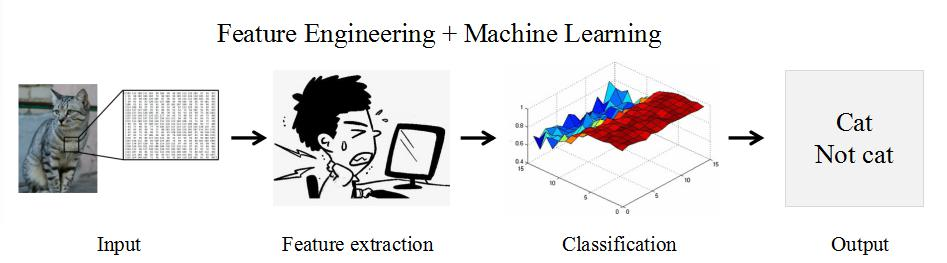
\includegraphics[width=8cm]{./Chapter5/Figures/feature-engineering.jpg}
    \end{minipage}%
    }
 \vfill
    \subfigure[端到端学习方法做图像分类]{
    \begin{minipage}{.9\textwidth}
        \centering
        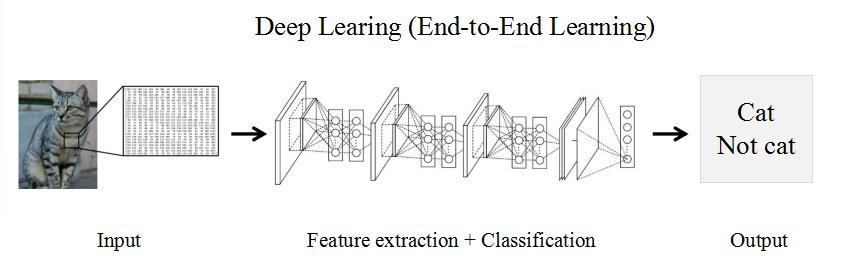
\includegraphics[width=8cm]{./Chapter5/Figures/deep-learning.jpg}
    \end{minipage}%
    }
\caption{特征工程{\small\sffamily\bfseries{vs}}端到端学习}
\label{fig:5-2}
\end {figure}
%------------------------------------------------------------------------------

\parinterval 传统的机器学习需要大量人工定义的特征,这些特征的构建往往会带来对问题的隐含假设。这种方法存在三方面的问题:

\begin{itemize}
\vspace{0.5em}
\item 特征的构造需要耗费大量的时间和精力。在传统机器学习的特征工程方法中,特征提取过程往往依赖于大量的先验假设,都基于人力完成的,这样导致相关系统的研发周期也大大增加;
\vspace{0.5em}
\item 最终的系统性能强弱非常依赖特征的选择。有一句话在业界广泛流传:``数据和特征决定了机器学习的上限'',但是人的智力和认知是有限的,因此人工设计的特征的准确性和覆盖度会受到限制;
\vspace{0.5em}
\item 通用性差。针对不同的任务,传统机器学习的特征工程方法需要选择出不同的特征,在这个任务上表现很好的特征在其他任务上可能没有效果。
\vspace{0.5em}
\end{itemize}

\parinterval 端到端学习将人们从大量的特征提取工作之中解放出来,可以不需要太多人的先验知识。从某种意义上讲,对问题的特征提取全是自动完成的,这也意味着哪怕我们不是该任务的``专家''也可以完成相关系统的开发。此外,端到端学习实际上也隐含了一种新的对问题的表示形式\ $\dash$\ {\small\bfnew{分布式表示}}\index{分布式表示}(Distributed Representation)\index{Distributed Representation}。在这种框架下,模型的输入可以被描述为分布式的实数向量,这样模型可以有更多的维度描述一个事物,同时避免传统符号系统对客观事物离散化的刻画。比如,在自然语言处理中,表示学习重新定义了什么是词,什么是句子。在本章后面的内容中也会看到,表示学习可以让计算机对语言文字的描述更加准确和充分。

%----------------------------------------------------------------------------------------
%    NEW SUBSUB-SECTION
%----------------------------------------------------------------------------------------

\subsubsection{深度学习的效果}

\parinterval 相比于传统的基于特征工程的方法,基于深度学习的模型更加方便、通用,在系统性能上也普遍更优。这里以语言建模任务为例。语言建模的目的是开发一个模型来描述词串出现的可能性(见第二章)。这个任务已经有着很长时间的历史。表\ref{tab:5-1}给出了不同方法在标准的PTB上的困惑度结果 \footnote{困惑度越低标明语言建模的效果越好。} 。传统的$ n$-gram语言模型由于面临维度灾难和数据稀疏问题,最终语言模型的性能并不是很好。而在深度学习模型中,通过引入循环神经网络等结构,所得到的语言模型可以更好地描述序列生成的问题。而最新的基于Transformer架构的语言模型将PPL从最初的178.0下降到了惊人的35.7。可见深度学习为这个任务所带来的进步是巨大的。

%----------------------------------------------------------------------------------------------------
\begin{table}[htp]
\centering
\caption{不同方法在PTB语言建模任务上的困惑度(PPL)}
\label{tab:5-1}
\small
\begin{tabular}{l | l l l}
\rule{0pt}{15pt}     模型 & 作者 & 年份 & PPL  \\
\hline
\rule{0pt}{15pt}     3-gram LM\cite{brown1992class} & Brown et al. & 1992 & 178.0  \\
\rule{0pt}{15pt}     Feed-forward Neural LM\cite{bengio2003neural} & Bengio et al. & 2003 & 162.2  \\
\rule{0pt}{15pt}     Recurrent NN-based LM\cite{mikolov2010recurrent} & Mikolov et al. & 2010 & 124.7  \\
\rule{0pt}{15pt}     Recurrent NN-LDA\cite{mikolov2012context} & Mikolov et al. & 2012 & 92.0  \\
\rule{0pt}{15pt}     LSTM \cite{zaremba2014recurrent}& Zaremba et al. & 2014 & 78.4  \\
\rule{0pt}{15pt}     RHN\cite{zilly2016recurrent} & Zilly et al. & 2016 & 65.4  \\
\rule{0pt}{15pt}     AWD-LSTM\cite{merity2017regularizing} & Merity et al. & 2018 & 58.8  \\
\rule{0pt}{15pt}     GPT-2 (Transformer)\cite{radford2019language} & Radford et al. & 2019 & 35.7  \\
\end{tabular}
\end{table}
%----------------------------------------------------------------------------------------------------

%----------------------------------------------------------------------------------------
%    NEW SECTION
%----------------------------------------------------------------------------------------

\sectionnewpage
\section{神经网络基础}

\parinterval 神经网络是一种由大量的节点(或称神经元)之间相互连接构成的计算模型。那么什么是神经元?神经元之间又是如何连接的?神经网络的数学描述又是什么样的?这一节将围绕这些问题对神经网络的基础知识进行系统的介绍。

%----------------------------------------------------------------------------------------
%    NEW SUB-SECTION
%----------------------------------------------------------------------------------------

\subsection{线性代数基础} \label{sec:5.2.1}

\parinterval 线性代数作为一个数学分支,广泛应用于科学和工程中,神经网络的数学描述中也大量使用了线性代数工具。因此,这里对线性代数的一些概念进行简要介绍,以方便后续对神经网络的数学建模。

%----------------------------------------------------------------------------------------
%    NEW SUBSUB-SECTION
%----------------------------------------------------------------------------------------

\subsubsection{标量、向量和矩阵}

\vspace{-0.5em}
\parinterval {\small\sffamily\bfseries{标量}}\index{标量}(Scalar)\index{Scalar}:标量亦称``无向量'',是一种只具有数值大小而没有方向的量,通俗地说,一个标量就是一个单独的数,这里特指实数\footnote{严格意义上,标量可以是复数等其他形式。这里为了方便讨论,仅以实数为对象。}。一般用小写斜体表示标量。比如,对于$ a=5 $,$ a $就是一个标量。

\parinterval {\small\sffamily\bfseries{向量}}\index{向量}(Vector)\index{Vector}:向量是由一组实数组成的有序数组。与标量不同,向量既有大小也有方向。可以把向量看作空间中的点,每个元素是不同坐标轴上的坐标。公式\ref{eq:5-1}和公式\ref{eq:5-2}展示了一个行向量和一个列向量。本章默认使用行向量,如$ \mathbf a=(a_1, a_2, a_3) $,$ \mathbf a $对应的列向量记为$ \mathbf a^{\rm T} $。
\begin{eqnarray}
\mathbf a &=& \begin{pmatrix}
  1 & 2 & 5 & 7
\end{pmatrix}\label{eq:5-1}\\ \nonumber \\
\mathbf{a^{\textrm{T}}} &=& \begin{pmatrix}
    &1& \\
    &2&\\
    &5& \\
    &7&\end{pmatrix}
\label{eq:5-2}
\end{eqnarray}

\parinterval {\small\sffamily\bfseries{矩阵}}\index{矩阵}(Matrix)\index{Matrix}:矩阵是一个按照长方阵列排列的实数集合,最早来自于方程组的系数及常数所构成的方阵。在计算机领域,通常将矩阵看作二维数组。我们用粗体的符号$ \mathbf a $表示一个矩阵,如果该矩阵有$ m $行$ n $列,那么有$ \mathbf a\in R^{m\times n} $。这里,用不加粗的符号来表示矩阵中的元素,其中每个元素都被一个行索引和一个列索引所确定。例如,$ a_{ij} $表示第$ i $行、第$ j $列的矩阵元素。如下,公式\ref{eq:5-3}中$ \mathbf a $定义了一个2行2列的矩阵。
\begin{eqnarray}
\mathbf a & = & \begin{pmatrix}
   a_{11} & a_{12}\\
   a_{21} & a_{22}
\end{pmatrix} \nonumber \\
& = & \begin{pmatrix}
   1 & 2\\
   3 & 4
\end{pmatrix}
\label{eq:5-3}
\end{eqnarray}

%----------------------------------------------------------------------------------------
%    NEW SUBSUB-SECTION
%----------------------------------------------------------------------------------------

\subsubsection{矩阵的转置}

\parinterval {\small\sffamily\bfseries{转置}}\index{转置}(Transpose)\index{Transpose}是矩阵的重要操作之一。矩阵的转置可以看作是将矩阵以对角线为镜像进行翻转:假设$ \mathbf a $为$ m $行$ n $列的矩阵,第$ i $行、第$ j $ 列的元素是$ a_{ij} $,即:$ \mathbf a={(a_{ij})}_{m\times n} $,把$ m\times n $矩阵$ \mathbf a $的行换成同序数的列得到一个$ n\times m $矩阵,则得到$ \mathbf a $的转置矩阵,记为$ \mathbf a^{\rm T} $,其中$ a_{ji}^{\rm T}=a_{ij} $。例如:
\begin{eqnarray}
\mathbf a & = & \begin{pmatrix} 1 & 3 & 2 & 6\\5 & 4 & 8 & 2\end{pmatrix} \\ \nonumber \\
{\mathbf a}^{\rm T} & = &\begin{pmatrix} 1 & 5\\3 & 4\\2 & 8\\6 & 2\end{pmatrix}
\end{eqnarray}

\parinterval 向量可以看作只有一行(列)的矩阵。对应地,向量的转置可以看作是只有一列(行)的矩阵。标量可以看作是只有一个元素的矩阵。因此,标量的转置等于它本身,即$ a^{\rm T}=a $。

%----------------------------------------------------------------------------------------
%    NEW SUBSUB-SECTION
%----------------------------------------------------------------------------------------

\subsubsection{矩阵加法和数乘}

\parinterval 矩阵加法又被称作{\small\sffamily\bfseries{按元素加法}}\index{按元素加法}(Element-wise Addition)\index{Element-wise Addition}。它是指两个矩阵把其相对应元素加在一起的运算,通常的矩阵加法被定义在两个形状相同的矩阵上。两个$ m\times n $矩阵$ \mathbf a $和$ \mathbf b $的和,标记为$ \mathbf a + \mathbf b $,它也是个$ m\times n $矩阵,其内的各元素为其相对应元素相加后的值。如果矩阵$ \mathbf c = \mathbf a + \mathbf b $,则$ c_{ij} = a_{ij} + b_{ij} $。公式\ref{eq:5-4}展示了矩阵之间进行加法的计算过程。
\begin{eqnarray}
\begin{pmatrix}
   1 & 3\\
   1 & 0\\
   1 & 2
\end{pmatrix}\;\;+\;\;\begin{pmatrix}
   0 & 0\\
   7 & 5\\
   2 & 1
\end{pmatrix}&=&\begin{pmatrix}
   1+0 & 3+0\\
   1+7 & 0+5\\
   1+2 & 2+1
\end{pmatrix}\;\;=\;\;\begin{pmatrix}
   1 & 3\\
   8 & 5\\
   3 & 3
\end{pmatrix}
\label{eq:5-4}
\end{eqnarray}

\parinterval 矩阵加法满足以下运算规律:

\begin{itemize}
\vspace{0.5em}
\item 交换律:$ \mathbf a+\mathbf b = \mathbf b +\mathbf a $。
\vspace{0.5em}
\item 结合律:$ (\mathbf a+\mathbf b)+\mathbf c = \mathbf a+(\mathbf b+\mathbf c) $。
\vspace{0.5em}
\item $ \mathbf a+\mathbf 0=\mathbf a $,其中$ \mathbf 0 $指的是零矩阵,即元素皆为0的矩阵。
\vspace{0.5em}
\item $ \mathbf a+(-\mathbf a)=\mathbf 0 $,其中$ -\mathbf a $是矩阵$ \mathbf a $的负矩阵,即将矩阵$ \mathbf a $的每个元素取负得到的矩阵。
\vspace{0.5em}
\end{itemize}

\parinterval 矩阵的{\small\bfnew{数乘}}\index{数乘}(Scalar Multiplication)\index{Scalar Multiplication}是指标量(实数)与矩阵的乘法运算,计算过程是将标量与矩阵的每个元素相乘,最终得到与原矩阵形状相同的矩阵。例如,矩阵$ \mathbf a={(a_{ij})}_{m\times n} $与标量$ k $进行数乘运算,其结果矩阵$ \mathbf b={(ka_{ij})}_{m\times n} $,即$ k{(a_{ij})}_{m\times n}={(ka_{ij})}_{m\times n} $。下面的式子展示了矩阵数乘的计算过程:
\begin{eqnarray}
\mathbf a & = &
\begin{pmatrix}
   3 & 2 & 7\\
   5 & 8 & 1
\end{pmatrix}
\\ \nonumber \\
2\mathbf a & = &
\begin{pmatrix}
   6 & 4 & 14\\
   10 & 16 & 2
\end{pmatrix}
\label{eq:5-5}
\end{eqnarray}

\parinterval 矩阵的数乘满足以下运算规律,其中$ k $和$ l $是实数,$ \mathbf a $和$ \mathbf b $是形状相同的矩阵:

\begin{itemize}
\vspace{0.5em}
\item 右分配律:$ k(\mathbf a+\mathbf b)=k\mathbf a+k\mathbf b $。
\vspace{0.5em}
\item 左分配律:$ (k+l)\mathbf a=k\mathbf a+l\mathbf a $。
\vspace{0.5em}
\item 结合律:$ (kl)\mathbf a=k(l\mathbf a) $。
%\vspace{0.5em}
\end{itemize}

%----------------------------------------------------------------------------------------
%    NEW SUBSUB-SECTION
%----------------------------------------------------------------------------------------

\subsubsection{矩阵乘法和矩阵点乘}

\parinterval 矩阵乘法是矩阵运算中最重要的操作之一,为了与矩阵点乘区分,通常也把矩阵乘法叫做矩阵叉乘。假设$ \mathbf a $为$ m\times p $的矩阵,$ \mathbf b $为$ p\times n $的矩阵,对$ \mathbf a $和$ \mathbf b $作矩阵乘法的结果是一个$ m\times n $的矩阵$ \mathbf c $,其中矩阵$ \mathbf c $中第$ i $行、第$ j $列的元素可以表示为:
\begin{eqnarray}
{(\mathbf a\mathbf b)}_{ij} &=& \sum_{k=1}^p a_{ik}b_{kj}
\label{eq:5-6}
\end{eqnarray}

\parinterval 只有当第一个矩阵的列数与第二个矩阵的行数相等时,两个矩阵才可以作矩阵乘法。公式\ref{eq:5-7}展示了矩阵乘法的运算过程,若$\mathbf a=\begin{pmatrix}a_{11} & a_{12}& a_{13}\\a_{21} & a_{22} & a_{23}\end{pmatrix}$,$\mathbf b=\begin{pmatrix}b_{11} & b_{12}\\b_{21} & b_{22}\\b_{31} & b_{32}\end{pmatrix} $,则有:
\vspace{-0.5em}
\begin{eqnarray}
\mathbf c & = & \mathbf a\mathbf b \nonumber \\
          & = & \begin{pmatrix}
   a_{11}b_{11}+a_{12}b_{21}+a_{13}b_{31} & a_{11}b_{12}+a_{12}b_{22}+a_{13}b_{32}\\
   a_{21}b_{11}+a_{22}b_{21}+a_{23}b_{31} & a_{21}b_{12}+a_{22}b_{22}+a_{23}b_{32}
\end{pmatrix}
\label{eq:5-7}
\end{eqnarray}

\parinterval 矩阵乘法满足以下运算规律:

\begin{itemize}
\vspace{0.5em}
\item 结合律:若$ \mathbf a\in R^{m\times n} $,$ \mathbf b\in R^{n\times p} $,$ \mathbf c\in R^{p\times q} $,则$ (\mathbf {ab})\mathbf c=\mathbf a(\mathbf {bc}) $。
\vspace{0.5em}
\item 左分配律:若$ \mathbf a\in R^{m\times n} $,$ \mathbf b\in R^{m\times n} $,$ \mathbf c\in R^{n\times p} $,则$ (\mathbf a+\mathbf b)\mathbf c=\mathbf {ac}+\mathbf {bc} $。
\vspace{0.5em}
\item 右分配律:若$ \mathbf a\in R^{m\times n} $,$ \mathbf b\in R^{n\times p} $,$ \mathbf c\in R^{n\times p} $,则$ \mathbf a(\mathbf b+\mathbf c)=\mathbf {ab}+\mathbf {ac} $。
\vspace{0.5em}
\end{itemize}

\begin{spacing}{1.4}
\parinterval 可以将线性方程组用矩阵乘法表示,如对于线性方程组$ \begin{cases} 5x_1+2x_2=y_1\\3x_1+x_2=y_2\end{cases} $,可以表示为$ \mathbf {ax}^{\rm T}=\mathbf y^{\rm T}$,其中$ \mathbf a = \begin{pmatrix} 5 & 2\\3 & 1\end{pmatrix} $,$ \mathbf x^{\rm T} = \begin{pmatrix} x_1\\x_2\end{pmatrix} $,$ \mathbf y^{\rm T} = \begin{pmatrix} y_1\\y_2\end{pmatrix} $。
\end{spacing}

\parinterval 矩阵的点乘就是两个形状相同的矩阵各个对应元素相乘,矩阵点乘也被称为{\small\bfnew{按元素乘积}}\index{按元素乘积}(Element-wise Product)\index{Element-wise Product}或Hadamard乘积,记为$ \mathbf a \odot \mathbf b$。例如,对于
\begin{eqnarray}
\mathbf a &=&
\begin{pmatrix}
   1 & 0\\
   -1 & 3
\end{pmatrix}
\\ \nonumber \\
\mathbf b &=&
\begin{pmatrix}
   3 & 1\\
   2 & 1
\end{pmatrix}
\end{eqnarray}

\parinterval 矩阵点乘的计算如下:
\begin{eqnarray}
\mathbf c & = & \mathbf a\odot \mathbf b \nonumber \\
          & = & \begin{pmatrix}
   1\times 3 & 0\times1\\
   -1\times2 & 3\times1
\end{pmatrix}
\label{eq:5-8}
\end{eqnarray}

%----------------------------------------------------------------------------------------
%    NEW SUBSUB-SECTION
%----------------------------------------------------------------------------------------

\subsubsection{线性映射}

\parinterval {\small\sffamily\bfseries{线性映射}}\index{线性映射}( Linear Mapping)\index{Linear Mapping}或{\small\sffamily\bfseries{线性变换}}\index{线性变换}(Linear Transformation)\index{Linear Transformation}是从一个向量空间V到另一个向量空间W的映射函数$ f:v\rightarrow w$,且该映射函数保持加法运算和数量乘法运算,即对于空间V中任何两个向量$ \mathbf u $ 和$ \mathbf v $以及任何标量$ c $,有:
\begin{eqnarray}
f(\mathbf u+\mathbf v)&=&f(\mathbf u)+f(\mathbf v)\label{eq:5-9}\\
f(c\mathbf v)&=&cf(\mathbf v)
\label{eq:5-10}
\end{eqnarray}

\parinterval 利用矩阵$ \mathbf a\in R^{m\times n} $,可以实现两个有限维欧氏空间的映射函数$f:R^n\rightarrow R^m$。例如$ n $维列向量$ \mathbf x ^{\rm T}$与$ m\times n $的矩阵$ \mathbf a $,向量$ \mathbf x ^{\rm T}$左乘矩阵$ \mathbf a $,可将向量$ \mathbf x ^{\rm T}$映射为$ m $列向量,对于
\begin{eqnarray}
\mathbf x^{\textrm{T}} & = & {\begin{pmatrix} x_1, & x_2, & \dots &, x_n \end{pmatrix}}^{\rm T}
\label{eq:5-11}
\end{eqnarray}

\begin{eqnarray}
\mathbf a&=&
\begin{pmatrix}
   a_{11} & a_{12} & \dots & a_{1n}\\
   a_{21} & \dots & \dots & \dots \\
   \dots & \dots & \dots & \dots \\
   a_{m1} & \dots & \dots & a_{mn}
\end{pmatrix}
\label{eq:5-12}
\end{eqnarray}

\parinterval 可以得到:
\begin{eqnarray}
\mathbf y^{\textrm{T}}& = &\mathbf a\mathbf x^{\textrm{T}} \nonumber \\
               & = &
\begin{pmatrix}
   a_{11}x_{1}+a_{12}x_{2}+\dots+a_{1n}x_{n}\\
   a_{21}x_{1}+a_{22}x_{2}+\dots+a_{2n}x_{n}\\
   \vdots \\
   a_{m1}x_{1}+a_{m2}x_{2}+\dots+a_{mn}x_{n}
\label{eq:5-13}\end{pmatrix}
\end{eqnarray}

\parinterval 上例中矩阵$ \mathbf a $定义了一个从$ R^n $到$ R^m $的线性映射:向量$ \mathbf x^{\textrm{T}}\in R^n $和$ \mathbf y^{\textrm{T}}\in R^m $别为两个空间中的列向量,即大小为$ n\times 1 $ 和$ m\times 1 $ 的矩阵。

%----------------------------------------------------------------------------------------
%    NEW SUBSUB-SECTION
%----------------------------------------------------------------------------------------

\subsubsection{范数}

\parinterval 工程领域,经常会使用被称为{\small\bfnew{范数}}\index{范数}(Norm)\index{Norm}的函数衡量向量大小,范数为向量空间内的所有向量赋予非零的正长度或大小。对于一个$n$维向量$ \mathbf x $,一个常见的范数函数为$ l_p $ 范数,通常表示为$ {\Vert{\mathbf x}\Vert}_p $ ,其中$p\ge 0$,是一个标量形式的参数。常用的$ p $的取值有$ 1 $、$ 2 $、$ \infty $等。范数的计算公式为:
\begin{eqnarray}
l_p(\mathbf x) & = & {\Vert{\mathbf x}\Vert}_p \nonumber \\
               & = & {\left (\sum_{i=1}^{n}{{\vert x_{i}\vert}^p}\right )}^{\frac{1}{p}}
\label{eq:5-14}
\end{eqnarray}

\parinterval $ l_1 $范数为向量的各个元素的绝对值之和:
\begin{eqnarray}
{\Vert{\mathbf x}\Vert}_1&=&\sum_{i=1}^{n}{\vert x_{i}\vert}
\label{eq:5-15}
\end{eqnarray}

\parinterval $ l_2 $范数为向量的各个元素平方和的二分之一次方:
\begin{eqnarray}
{\Vert{\mathbf x}\Vert}_2&=&\sqrt{\sum_{i=1}^{n}{{x_{i}}^2}} \nonumber \\
                                      &=&\sqrt{{\mathbf x}^{\rm T}\mathbf x}
\label{eq:5-16}
\end{eqnarray}

\parinterval $ l_2 $范数被称为{\small\bfnew{欧几里得范数}}\index{欧几里得范数}(Euclidean Norm)\index{Euclidean Norm}。从几何角度,向量也可以表示为从原点出发的一个带箭头的有向线段,其$ l_2 $范数为线段的长度,也常被称为向量的模。$ l_2 $ 范数在机器学习中非常常用,向量$ \mathbf x $的$ l_2 $范数经常简化为$ \Vert{\mathbf x}\Vert $,可以简单地通过点积$ {\mathbf x}^{\rm T}\mathbf x $计算。

\parinterval $ l_{\infty} $范数为向量的各个元素的最大绝对值:
\begin{eqnarray}
{\Vert{\mathbf x}\Vert}_{\infty}&=&{\rm{max}}\{x_1,x_2,\dots,x_n\}
\label{eq:5-17}
\end{eqnarray}

\parinterval 广义上讲,范数是将向量映射到非负值的函数,其作用是衡量向量$ \mathbf x $到坐标原点的距离。更严格的说,范数并不拘于$ l_p $范数,任何一个同时满足下列性质的函数都可以作为范数:

\begin{itemize}
\vspace{0.5em}
\item 若$ f(x)=0 $,则$ x=0 $。
\vspace{0.5em}
\item 三角不等式:$ f(x+y)\leqslant f(x)+f(y) $。
\vspace{0.5em}
\item 任意实数$ \alpha $,$ f(\alpha x)=\vert \alpha \vert f(x) $。
\vspace{0.5em}
\end{itemize}

\parinterval 在深度学习中,有时候希望衡量矩阵的大小,这时可以考虑使用 {\small\bfnew{Frobenius 范数}}\index{Frobenius 范数}(Frobenius Norm)\index{Frobenius Norm}。计算方式为:
\begin{eqnarray}
{\Vert{\mathbf a}\Vert}_F&=&\sqrt{\sum_{i,j} a_{i,j}^2}
\label{eq:5-18}
\end{eqnarray}

%----------------------------------------------------------------------------------------
%    NEW SUB-SECTION
%----------------------------------------------------------------------------------------
\subsection{人工神经元和感知机}

\parinterval 生物学中,神经元是神经系统的基本组成单元。图\ref{fig:5-3}展示了一个生物神经元实例。

%----------------------------------------------
\begin{figure}[htp]
\centering
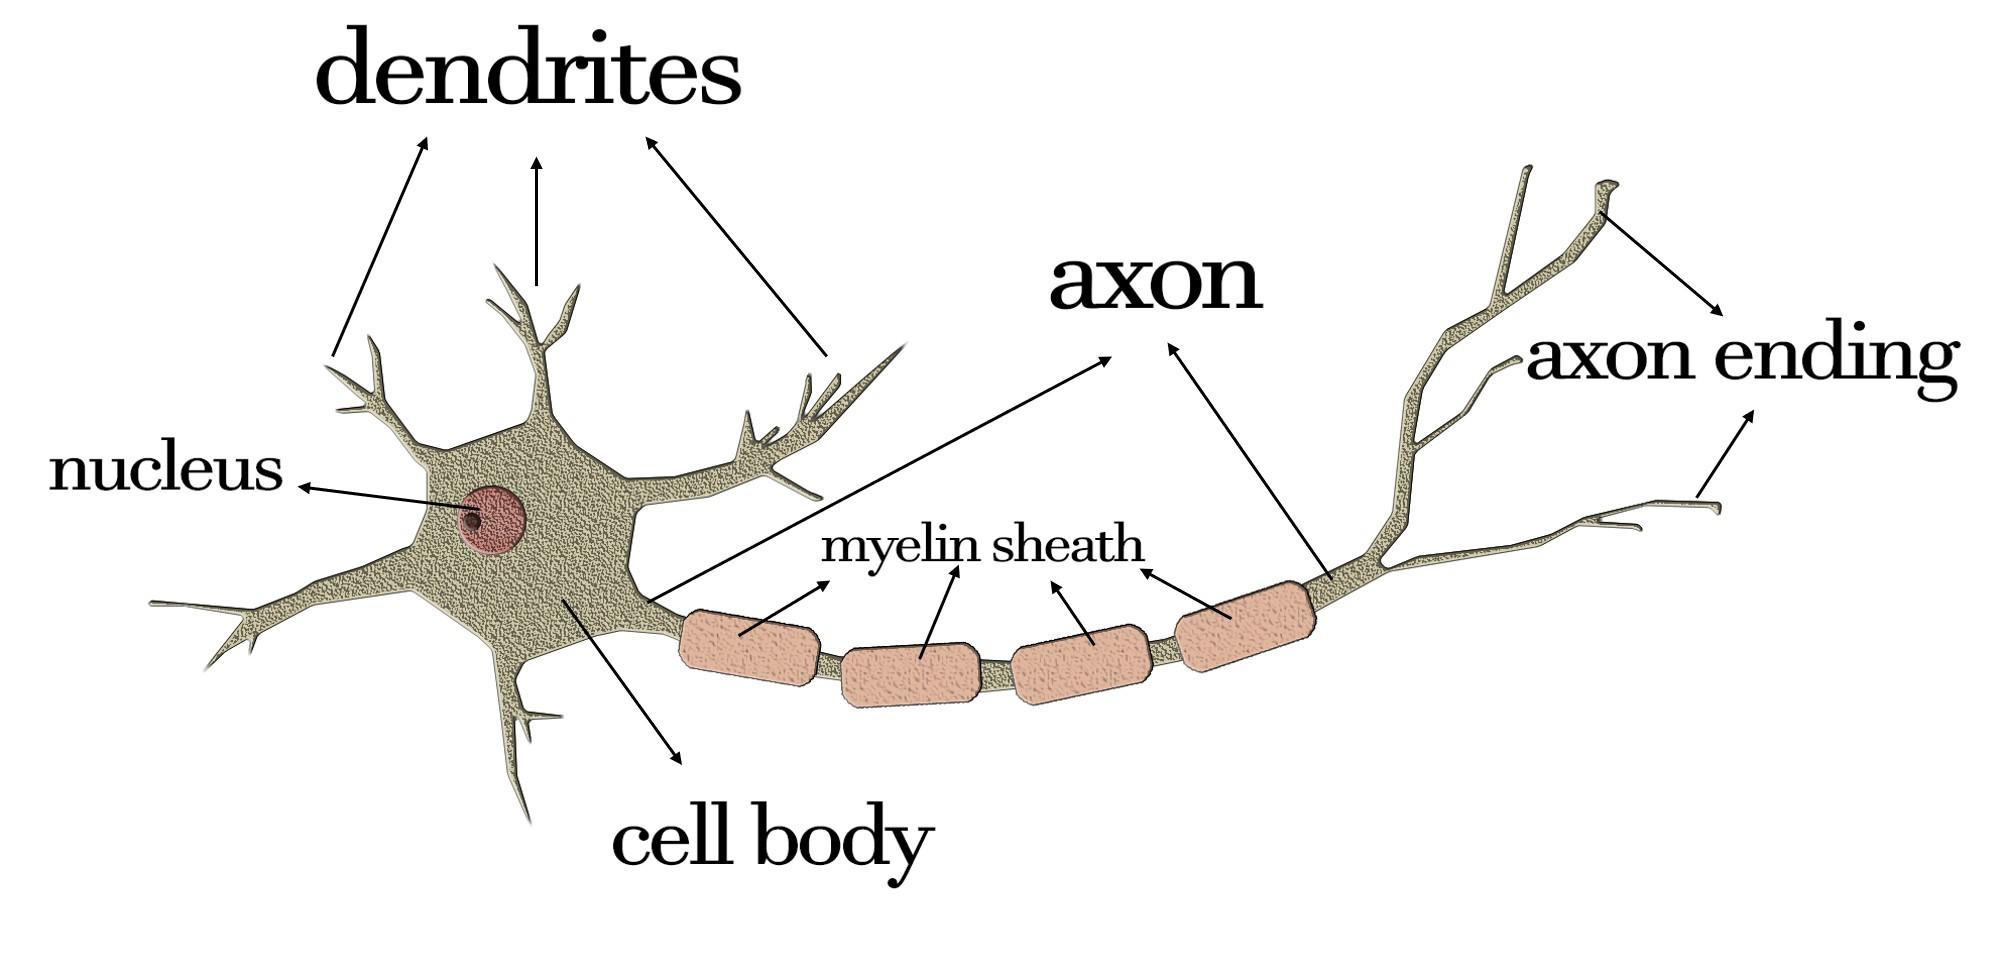
\includegraphics[width=8cm]{./Chapter5/Figures/biological-neuron.jpg}
\caption{生物神经元}
\label{fig:5-3}
\end{figure}
%-------------------------------------------

\parinterval 同样,人工神经元是人工神经网络的基本单元。在人们的想象中,人工神经元应该与生物神经元类似。但事实上,二者在形态上是有明显差别的。如图\ref{fig:5-4} 是一个典型的人工神经元,其本质是一个形似$ y=f(\mathbf x\cdot \mathbf w+b) $的函数。显而易见,一个神经元主要由$ \mathbf x $,$ \mathbf w $,$ b $,$ f $四个部分构成。其中$ \mathbf x $是一个形如$ (x_0,x_1,\dots,x_n) $ 的实数向量,在一个神经元中担任``输入''的角色。$ \mathbf w $是一个权重矩阵,其中的每一个元素都对应着一个输入和一个输出,代表着``某输入对某输出的贡献程度'',通常也被理解为神经元连接的{\small\sffamily\bfseries{权重}}\index{权重}(weight)\index{weight}。$ b $被称作偏置,是一个实数。$ f $被称作激活函数,其本质是一个非线性函数。可见,一个人工神经元的功能是将输入向量与权重矩阵右乘(做内积)后,加上偏置量,经过一个非线性激活函数得到一个标量结果。

%----------------------------------------------
\begin{figure}[htp]
\centering
%%%------------------------------------------------------------------------------------------------------------
\begin{tikzpicture}
\begin{scope}
\node [anchor=center,circle,draw,ublue,very thick,minimum size=3.5em,fill=white,drop shadow={shadow xshift=0.1em,shadow yshift=-0.1em}] (neuron) at (0,0) {};
\node [anchor=east] (x1) at ([xshift=-6em]neuron.west) {\Large{$x_1$}};
\node [anchor=center] (x0) at ([yshift=3em]x1.center) {\Large{$x_0$}};
\node [anchor=center] (x2) at ([yshift=-3em]x1.center) {\Large{$b$}};
\node [anchor=west] (y) at ([xshift=6em]neuron.east) {\Large{$y$}};
\node [anchor=center] (neuronmath) at (neuron.center) {\Large{$f$}};

\draw [->,thick] (x0.east) -- (neuron.150) node [pos=0.5,above] {$w_0$};
\draw [->,thick] (x1.east) -- (neuron.180) node [pos=0.5,above] {$w_1$};
\draw [->,thick] (x2.east) -- (neuron.210) node [pos=0.5,above] {$$};
\draw [->,thick] (neuron.east) -- (y.west);

\end{scope}
\end{tikzpicture}
%
%%%------------------------------------------------------------------------------------------------------------


\caption{人工神经元}
\label{fig:5-4}
\end{figure}
%----------------------------------------------

%----------------------------------------------------------------------------------------
%    NEW SUBSUB-SECTION
%----------------------------------------------------------------------------------------

\vspace{-0.5em}
\subsubsection{感知机\ \dash \ 最简单的人工神经元模型}

\vspace{0.5em}
\parinterval 感知机是人工神经元的一种实例,在上世纪50-60年代被提出后,对神经网络研究产生了深远的影响。感知机模型如图\ref {fig:5-5}所示,其输入是一个$n$维二值向量$ \mathbf x=(x_0,x_1,\dots,x_n) $,其中$ x_i=0 $或$ 1 $。权重$ \mathbf w=(w_0,w_1,\dots,w_n) $,每个输入变量对应一个权重$ w_i $(实数)。偏置$ b $是一个实数变量($ -\sigma $)。输出也是一个二值结果,即$ y=0 $或$ 1 $。$ y $值的判定由输入的加权和是否大于(或小于)一个阈值$ \sigma $决定(公式\ref{eq:5-19}):
\begin{eqnarray}
y=\begin{cases} 0 & \sum_{i}{x_i\cdot w_i}-\sigma <0\\1 & \sum_{i}{x_i\cdot w_i}-\sigma \geqslant 0\end{cases}
\label{eq:5-19}
\end{eqnarray}

%----------------------------------------------
\begin{figure}[htp]
\centering
%%%------------------------------------------------------------------------------------------------------------
 \begin{tikzpicture}
\begin{scope}
\node [anchor=center,circle,draw,ublue,very thick,minimum size=3.5em,fill=white,drop shadow={shadow xshift=0.1em,shadow yshift=-0.1em}] (neuron) at (0,0) {};
\node [anchor=east] (x1) at ([xshift=-6em]neuron.west) {\Large{$x_1$}};
\node [anchor=center] (x0) at ([yshift=3em]x1.center) {\Large{$x_0$}};
\node [anchor=center] (x2) at ([yshift=-3em]x1.center) {\Large{$x_2$}};
\node [anchor=west] (y) at ([xshift=6em]neuron.east) {\Large{$y$}};
\node [anchor=center] (neuronmath) at (neuron.center) {\red{\small{$\sum \ge \sigma$}}};

\draw [->,thick] (x0.east) -- (neuron.150) node [pos=0.5,above] {$w_0$};
\draw [->,thick] (x1.east) -- (neuron.180) node [pos=0.5,above] {$w_1$};
\draw [->,thick] (x2.east) -- (neuron.210) node [pos=0.5,above] {$w_2$};
\draw [->,thick] (neuron.east) -- (y.west);

\end{scope}
\end{tikzpicture}
%%%------------------------------------------------------------------------------------------------------------


\caption{感知机模型}
\label{fig:5-5}
\end{figure}
%-------------------------------------------

\parinterval 感知机可以做一些简单的决策。举一个非常简单的例子,有一场音乐会,你正在纠结是否去参加,有三个因素会影响你的决定:

\begin{itemize}
\vspace{0.5em}
\item $ x_0 $:剧场是否离你足够近(是,则$ x_0=1 $;否则$ x_0=0 $);
\vspace{0.5em}
\item $ x_1 $:票价是否低于300元(是,则$ x_1=1 $;否则$ x_1=0 $);
\vspace{0.5em}
\item $ x_2 $:女朋友是否喜欢音乐会(是,则$ x_2=1 $;否则$ x_2=0 $)。
\vspace{0.5em}
\end{itemize}

\parinterval 在这种情况下应该如何做出决定呢?比如,女朋友很希望和你一起去看音乐会,但是剧场很远而且票价500元,如果这些因素对你都是同等重要的(即$ w_0=w_1=w_2 $,假设这三个权重都设置为1)那么会得到一个综合得分:
\begin{eqnarray}
x_0\cdot w_0+x_1\cdot w_1+x_2\cdot w_2 & = & 0\cdot 1+0\cdot 1+1\cdot 1 \nonumber \\
                                                                     & = & 1
\label{eq:5-20}
\end{eqnarray}

\parinterval 如果你不是十分纠结的人,能够接受不完美的事情,你可能会把$ \sigma $设置为1,于是$ \sum{w_i\cdot x_i}-\sigma \ge 0 $,那么你会去音乐会。可以看出,上面的例子的本质就是一个如图\ref{fig:5-6}的感知机:

%----------------------------------------------
\begin{figure}[htp]
\centering
%%%------------------------------------------------------------------------------------------------------------
 \begin{tikzpicture}
\begin{scope}
\node [anchor=center,circle,draw,ublue,very thick,minimum size=3.5em,fill=white,drop shadow={shadow xshift=0.1em,shadow yshift=-0.1em}] (neuron) at (0,0) {};
\node [anchor=east] (x1) at ([xshift=-6em]neuron.west) {$x_1$:票价够低?};
\node [anchor=center] (x0) at ([yshift=3em]x1.center) {$x_0$:距离够近?};
\node [anchor=center] (x2) at ([yshift=-3em]x1.center) {$x_2$:女友喜欢?};
\node [anchor=west] (y) at ([xshift=2em]neuron.east) {$y$:去?还是不去?};

{
\draw [->,thick] (x0.east) -- (neuron.150) node [pos=0.5,above,yshift=0.2em] {\small{$w_0=1$}};
\draw [->,thick] (x1.east) -- (neuron.180) node [pos=0.5,above,yshift=-0.1em] {\small{$w_1=1$}};
\draw [->,thick] (x2.east) -- (neuron.210) node [pos=0.5,above,yshift=0.1em] {\small{$w_2=1$}};
}
\draw [->,thick] (neuron.east) -- (y.west);

\node [anchor=center] (neuronmath) at (neuron.center) {\small{$\sum \ge \sigma$}};

\end{scope}
\end{tikzpicture}
%%%------------------------------------------------------------------------------------------------------------



\caption{预测是否去剧场的感知机(权重相同)}
\label{fig:5-6}
\end{figure}
%-------------------------------------------

%----------------------------------------------------------------------------------------
%    NEW SUBSUB-SECTION
%----------------------------------------------------------------------------------------

\vspace{-1em}
\subsubsection{神经元内部权重}

\parinterval 在上面的例子中,连接权重代表着每个输入因素对最终输出结果的重要程度,为了得到令人满意的决策,需要不断调整权重。如果你是守财奴,则会对票价看得更重一些,这样你会用不均匀的权重计算每个因素的影响,比如:$ w_0=0.5 $,$ w_1=2 $,$ w_2=0.5 $,此时感知机模型如图\ref{fig:5-7}所示。在这种情况下,女友很希望和你一起去看音乐会,但是剧场很远而且票价500元,会导致你不去看音乐会,因为
\begin{eqnarray}
\sum_{i}{x_i\cdot w_i} & = & 0\cdot 0.5+0\cdot 2+1\cdot 0.5 \nonumber \\
                                   & = & 0.5 \nonumber \\
                                   & < & \sigma = 1
\label{eq:5-21}
\end{eqnarray}

%----------------------------------------------
\begin{figure}[htp]
\centering
%%%------------------------------------------------------------------------------------------------------------
\begin{tikzpicture}
\begin{scope}
\node [anchor=center,circle,draw,ublue,very thick,minimum size=3.5em,fill=white,drop shadow={shadow xshift=0.1em,shadow yshift=-0.1em}] (neuron) at (0,0) {};
\node [anchor=east] (x1) at ([xshift=-6em]neuron.west) {$x_1$:票价够低?};
\node [anchor=center] (x0) at ([yshift=3em]x1.center) {$x_0$:距离够近?};
\node [anchor=center] (x2) at ([yshift=-3em]x1.center) {$x_2$:女友喜欢?};
\node [anchor=west] (y) at ([xshift=2em]neuron.east) {$y$:去?还是不去?};


\draw [->,thin] (x0.east) -- (neuron.150) node [pos=0.5,above,yshift=0.2em] {\small{$w_0=.5$}};
\draw [->,line width=0.5mm] (x1.east) -- (neuron.180) node [pos=0.5,above,yshift=-0.1em] {\textbf{\small{$w_1=2$}}};
\draw [->,thin] (x2.east) -- (neuron.210) node [pos=0.5,above,yshift=0.1em] {\small{$w_2=.5$}};
\draw [->,thick] (neuron.east) -- (y.west);

\node [anchor=center] (neuronmath) at (neuron.center) {\small{$\sum \ge \sigma$}};
\node [anchor=south] (ylabel) at (y.north) {\textbf{不去了!}};


\end{scope}
\end{tikzpicture}
%%%------------------------------------------------------------------------------------------------------------



\caption{预测是否去剧场的感知机(改变权重)}
\label{fig:5-7}
\end{figure}
%-------------------------------------------

\parinterval 当然,结果是女友对这个决定非常不满意,让你跪键盘上反思一下自己。

%----------------------------------------------------------------------------------------
%    NEW SUBSUB-SECTION
%----------------------------------------------------------------------------------------

\subsubsection{神经元的输入\ \dash \ 离散 vs 连续}

\parinterval 在遭受了女友一万点伤害之后,你意识到决策考虑的因素(即输入)不应该只是非0即1,而应该把``程度''考虑进来,于是你改变了三个输入的形式:

\parinterval $ x_0 $:10/距离

\parinterval $ x_1 $:150/票价

\parinterval $ x_2 $:女朋友是否喜欢

\parinterval 在新修改的模型中,$ x_0 $和$ x_1 $变成了连续变量,$ x_2 $仍然是离散变量,如图\ref{fig:5-8}。

%----------------------------------------------
\begin{figure}[htp]
\centering
%%%------------------------------------------------------------------------------------------------------------
\begin{tikzpicture}

\begin{scope}
\draw [->,thick] (0,0) -- (2.5,0);
\draw [->,thick] (0,0) -- (0, 1.5);
\draw [-,very thick,ublue,domain=0.6:2,samples=100] plot (\x,{ 1/\x - 0.2});
\node [anchor=east] (ylabel) at (0, 3.2em) {\footnotesize{$x_0$}};
\node [anchor=north] (xlabel) at (5em, 0em) {\scriptsize{距离(km)}};
\end{scope}

\begin{scope}[xshift=9em]
\draw [->,thick] (0,0) -- (2.5,0);
\draw [->,thick] (0,0) -- (0, 1.5);
\draw [-,very thick,ublue,domain=0.4:2,samples=100] plot (\x,{ 0.5/\x});
\node [anchor=east] (ylabel) at (0, 3.2em) {\footnotesize{$x_1$}};
\node [anchor=north] (xlabel) at (5em, 0em) {\scriptsize{票价(元)}};
\end{scope}

\begin{scope}[xshift=18em]
\draw [->,thick] (0,0) -- (2.5,0);
\draw [->,thick] (0,0) -- (0, 1.5);
\node [anchor=east] (ylabel) at (0, 3.2em) {\footnotesize{$x_2$}};
\node [anchor=south, fill=ublue, minimum width=1.5em, minimum height=0.1em, inner sep=0] (histogram1) at (1.5em, 0) {};
\node [anchor=south, fill=ublue, minimum width=1.5em, minimum height=3em, inner sep=0] (histogram2) at (4.0em, 0) {};
\node [anchor=north] (hlabel1) at (histogram1.south) {\tiny{女友不去}};
\node [anchor=north] (hlabel2) at (histogram2.south) {\tiny{女友去}};
\end{scope}

\end{tikzpicture}
%%%------------------------------------------------------------------------------------------------------------



\caption{神经元输入的不同形式}
\label{fig:5-8}
\end{figure}
%-------------------------------------------

\parinterval 使用修改后的模型做决策:女朋友很希望和你一起,但是剧场有20km远而且票价有500元。于是有$ x_0=10/20 $,$ x_1=150/500 $,$ x_2=1 $。
\begin{eqnarray}
\sum_{i}{x_i\cdot w_i} & = & 0.5\cdot 0.5+0.3\cdot 2+1\cdot 0.5 \nonumber \\
                                   & = & 1.35 \nonumber \\
                                   & > & \sigma =1
\label{eq:5-22}
\end{eqnarray}

\parinterval 虽然剧场很远,价格有点贵,但是女友很满意,你还是很高兴。

%----------------------------------------------------------------------------------------
%    NEW SUBSUB-SECTION
%----------------------------------------------------------------------------------------

\subsubsection{神经元内部的参数学习}

\parinterval 一次成功的音乐会之后,你似乎掌握了一个真理:其他什么都不重要,女友的喜好最重要,所以你又将决策模型的权重做出了调整:最简单的方式就是$ w_0=w_1=0 $,同时令$ w_2>0 $,相当于只考虑$ x_2 $的影响而忽略其他因素,于是你得到了如图\ref {fig:5-9}所示的决策模型:

%----------------------------------------------
\begin{figure}[htp]
\centering
%%%------------------------------------------------------------------------------------------------------------
\begin{tikzpicture}
\begin{scope}
\node [anchor=center,circle,draw,ublue,very thick,minimum size=3.5em,fill=white,drop shadow={shadow xshift=0.1em,shadow yshift=-0.1em}] (neuron) at (0,0) {};
\node [anchor=east] (x1) at ([xshift=-6em]neuron.west) {$x_1$:便宜程度\ \ \ \ };
\node [anchor=center] (x0) at ([yshift=3em]x1.center) {$x_0$:远近程度\ \ \ \ };
\node [anchor=center] (x2) at ([yshift=-3em]x1.center) {$x_2$:女友喜欢?};
\node [anchor=west] (y) at ([xshift=2em]neuron.east) {$y$:去?还是不去?};

\draw [->,thick] (neuron.east) -- (y.west);

\node [anchor=center] (neuronmath) at (neuron.center) {\small{$\sum \ge \sigma$}};

{
\draw [->,dotted] (x0.east) -- (neuron.150) node [pos=0.5,above,yshift=0.2em] {\small{$w_0=0$}};
\draw [->,dotted] (x1.east) -- (neuron.180) node [pos=0.5,above,yshift=-0.1em] {\textbf{\small{$w_1=0$}}};
\draw [->,line width=0.5mm] (x2.east) -- (neuron.210) node [pos=0.5,above,yshift=0.1em] {\small{$w_2=10$}};
}


\end{scope}
\end{tikzpicture}
%%%------------------------------------------------------------------------------------------------------------



\caption{预测是否去剧场的决策模型(只考虑女友喜好)}
\label{fig:5-9}
\end{figure}
%-------------------------------------------

\parinterval 很快又有了一场音乐会,距你1000公里,票价3000元,当然女友是一直喜欢音乐会的。根据新的决策模型,你义无反顾地选择去看音乐会。然而,女友又不高兴了,喜欢浪漫的女友觉得去看这场音乐会太奢侈了。在这几次看音乐会的经历中,你发现每个因素的权重需要准确地设置才能达到最好的决策效果。

\parinterval 那么如何确定最好的权重的?方法其实很简单,不断地尝试,根据结果不断地调整权重。在经过成百上千次的尝试之后,终于找到了一组合适的权重,使每次决策的正确率都很高。上面这个过程就类似于参数训练的过程,利用大量的数据来模拟成百上千次的尝试,根据输出的结果来不断地调整权重。

\parinterval 可以看到,在``是否参加音乐会''这个实际问题中,主要涉及到三方面的问题:

\begin{itemize}
\vspace{0.5em}
\item 对问题建模,即定义输入$ \{x_i\} $的形式;
\vspace{0.5em}
\item 设计有效的决策模型,即定义$ y $;
\vspace{0.5em}
\item 决定模型所涉及的参数(如权重$ \{w_i\} $)的最优值。
\vspace{0.5em}
\end{itemize}

\parinterval 上面的例子对这三个问题都简要地做出了回答。下面的内容将继续对它们进行详细阐述。

%----------------------------------------------------------------------------------------
%    NEW SUB-SECTION
%----------------------------------------------------------------------------------------

\subsection{多层神经网络}

\parinterval 感知机是一种最简单的单层神经网络。一个非常自然的问题是:能否把多个这样的网络叠加在一起,获得建模更复杂问题的能力?如果可以,那么在多层神经网络的每一层,神经元之间是怎么组织、工作的呢?单层网络又是通过什么方式构造成多层的呢?

%----------------------------------------------------------------------------------------
%    NEW SUBSUB-SECTION
%----------------------------------------------------------------------------------------

\subsubsection{线性变换和激活函数}

\parinterval 为了建立多层神经网络,首先需要把前面提到的简单的神经元进行扩展,把多个神经元组成一``层''神经元。比如,很多实际问题需要同时有多个输出,这时可以把多个相同的神经元并列起来,每个神经元都会有一个单独的输出,这就构成一``层'',形成了单层神经网络。单层神经网络中的每一个神经元都对应着一组权重和一个输出,可以把单层神经网络中的不同输出看作一个事物不同角度的描述。

%----------------------------------------------
\begin{figure}[htp]
\centering
%%%------------------------------------------------------------------------------------------------------------
\begin{tikzpicture}
\begin{scope}

\tikzstyle{neuronnode} = [minimum size=1.5em,circle,draw,ublue,very thick,fill=white,drop shadow={shadow xshift=0.1em,shadow yshift=-0.1em}]

\node [anchor=center,neuronnode] (neuron00) at (0,0) {};
\node [anchor=center,neuronnode] (neuron01) at ([yshift=-3em]neuron00) {};
\node [anchor=center,neuronnode] (neuron02) at ([yshift=-3em]neuron01) {};

\node [anchor=east] (x0) at ([xshift=-6em]neuron00.west) {$x_0$};
\node [anchor=east] (x1) at ([xshift=-6em]neuron01.west) {$x_1$};
\node [anchor=east] (x2) at ([xshift=-6em]neuron02.west) {$b$};

\node [anchor=west] (y0) at ([xshift=4em]neuron00.east) {$y_0$:\scriptsize{温度}};

\draw [->,red!50,line width=0.4mm] (x0.east) -- (neuron00.180) node [pos=0.1,above] {\tiny{$w_{00}$}};
\draw [->,red!50,line width=0.4mm] (x1.east) -- (neuron00.200) node [pos=0.1,above] {\tiny{$w_{10}$}};
\draw [->,red!50,line width=0.4mm] (x2.east) -- (neuron00.220) node [pos=0.05,above,yshift=0.3em] {\tiny{$b_{0}$}};
\draw [->,red!30,line width=0.4mm] (neuron00.east) -- (y0.west);

\node [anchor=west] (y1) at ([xshift=4em]neuron01.east) {$y_1$:\scriptsize{湿度}};

\draw [->,blue!50,line width=0.4mm] (x0.east) -- (neuron01.160) node [pos=0.4,above] {\tiny{$w_{01}$}};
\draw [->,blue!50,line width=0.4mm] (x1.east) -- (neuron01.180) node [pos=0.35,above,yshift=-0.2em] {\tiny{$w_{11}$}};
\draw [->,blue!50,line width=0.4mm] (x2.east) -- (neuron01.200) node [pos=0.3,below,yshift=0.2em] {\tiny{$b_{1}$}};
\draw [->,blue!30,line width=0.4mm] (neuron01.east) -- (y1.west);

\node [anchor=west] (y2) at ([xshift=4em]neuron02.east) {$y_2$:\scriptsize{风力}};

\draw [->,purple!40,line width=0.4mm] (x0.east) -- (neuron02.140) node [pos=0.1,below,yshift=-0.2em] {\tiny{$w_{02}$}};
\draw [->,purple!40,line width=0.4mm] (x1.east) -- (neuron02.160) node [pos=0.1,below] {\tiny{$w_{12}$}};
\draw [->,purple!40,line width=0.4mm] (x2.east) -- (neuron02.180) node [pos=0.3,below] {\tiny{$b_{2}$}};
\draw [->,purple!30,line width=0.4mm] (neuron02.east) -- (y2.west);

\end{scope}
\end{tikzpicture}



%%%------------------------------------------------------------------------------------------------------------


\caption{权重矩阵中的元素与输出的对应关系}
\label{fig:5-10}
\end{figure}
%-------------------------------------------

\parinterval 举个简单的例子,预报天气时,往往需要预测温度、湿度和风力,这就意味着如果使用单层神经网络进行预测,需要设置3个神经元。如图\ref{fig:5-10},权重矩阵为:
\begin{eqnarray}
\mathbf w=\begin{pmatrix} w_{00} & w_{01} & w_{02}\\ w_{10} & w_{11} & w_{12}\end{pmatrix}
\end{eqnarray}

\noindent 它的第一列元素$ \begin{pmatrix} w_{00}\\ w_{10}\end{pmatrix} $是输入相对第一个输出$ y_0 $ 的权重,参数向量$ \mathbf b=(b_0,b_1,b_2) $的第一个元素$ b_0 $是对应于第一个输出$ y_0 $ 的偏置量;类似的,可以得到$ y_1 $和$ y_2 $。预测天气的单层模型如图\ref{fig:5-11}所示(在本例中,假设输入$ \mathbf x=(x_0,x_1) $)。

%----------------------------------------------
\begin{figure}[htp]
\centering
%%%------------------------------------------------------------------------------------------------------------
\begin{tikzpicture}
\begin{scope}

\tikzstyle{neuronnode} = [minimum size=1.5em,circle,draw,ublue,very thick,fill=white,drop shadow={shadow xshift=0.1em,shadow yshift=-0.1em}]

\node [anchor=center,neuronnode] (neuron00) at (0,0) {};
\node [anchor=center,neuronnode] (neuron01) at ([yshift=-3em]neuron00) {};
\node [anchor=center,neuronnode] (neuron02) at ([yshift=-3em]neuron01) {};
\node [anchor=east] (x0) at ([xshift=-6em]neuron00.west) {$x_0$};
\node [anchor=east] (x1) at ([xshift=-6em]neuron01.west) {$x_1$};
\node [anchor=east] (x2) at ([xshift=-6em]neuron02.west) {$b$};
\node [anchor=west] (y0) at ([xshift=4em]neuron00.east) {$y_0$};

\draw [->] (x0.east) -- (neuron00.180) node [pos=0.1,above] {\tiny{$w_{00}$}};
\draw [->] (x1.east) -- (neuron00.200) node [pos=0.1,above] {\tiny{$w_{10}$}};
\draw [->] (x2.east) -- (neuron00.220) node [pos=0.05,above,yshift=0.3em] {\tiny{$b_{0}$}};
\draw [->] (neuron00.east) -- (y0.west);

\node [anchor=west] (y1) at ([xshift=4em]neuron01.east) {$y_1$};
\draw [->] (x0.east) -- (neuron01.160) node [pos=0.4,above] {\tiny{$w_{01}$}};
\draw [->] (x1.east) -- (neuron01.180) node [pos=0.35,above,yshift=-0.2em] {\tiny{$w_{11}$}};
\draw [->] (x2.east) -- (neuron01.200) node [pos=0.3,below,yshift=0.2em] {\tiny{$b_{1}$}};
\draw [->] (neuron01.east) -- (y1.west);

\node [anchor=west] (y2) at ([xshift=4em]neuron02.east) {$y_2$};
\draw [->] (x0.east) -- (neuron02.140) node [pos=0.1,below,yshift=-0.2em] {\tiny{$w_{02}$}};
\draw [->] (x1.east) -- (neuron02.160) node [pos=0.1,below] {\tiny{$w_{12}$}};
\draw [->] (x2.east) -- (neuron02.180) node [pos=0.3,below] {\tiny{$b_{2}$}};
\draw [->] (neuron02.east) -- (y2.west);

\node [anchor=east,align=left] (inputlabel) at ([xshift=-0.1em]x1.west) {\scriptsize{输入向量}:\\\small{$\textbf{x}=(x_0,x_1)$}};


\node [anchor=west,align=left] (outputlabel) at ([xshift=0.1em]y1.east) {\scriptsize{输出向量}:\\\small{$\textbf{y}=(y_0,y_1,y_2)$}};


\begin{pgfonlayer}{background}

\node [rectangle,inner sep=0.4em,fill=red!20] [fit = (neuron00) (neuron01) (neuron02)] (layer) {};
\node [anchor=south] (layerlabel) at ([yshift=0.2em]layer.north) {\scriptsize{一层神经元}};



\node [rectangle,inner sep=0.1em,fill=ugreen!20] [fit = (x0) (x1)] (inputshadow) {};


\node [rectangle,inner sep=0.1em,fill=blue!20] [fit = (y0) (y1) (y2)] (outputshadow) {};

\end{pgfonlayer}



\end{scope}
\end{tikzpicture}
%%%------------------------------------------------------------------------------------------------------------


\caption{预测天气的单层神经网络}
\label{fig:5-11}
\end{figure}
%-------------------------------------------

\parinterval 在神经网络中,对于输入向量$ \mathbf x\in R^m $,一层神经网络首先将其经过线性变换映射到$ R^n $,再经过激活函数变成$  \mathbf y\in R^n $。还是上面天气预测的例子,每个神经元获得相同的输入,权重矩阵$ \mathbf w $是一个$ 2\times 3 $矩阵,矩阵中每个元素$ w_{ij} $代表第$ j $个神经元中$ x_{i} $对应的权重值,假设编号为0的神经元负责预测温度,则$ w_{i0} $含义为预测温度时,输入$ x_{i} $对其影响程度。此外所有神经元的偏置$ b_{0} $,$ b_{1} $,$ b_{2} $组成了最终的偏置向量$ \mathbf b $。在该例中则有,权重矩阵$ \mathbf w=\begin{pmatrix} w_{00} & w_{01} & w_{02}\\ w_{10} & w_{11} & w_{12}\end{pmatrix} $,偏置向量$ \mathbf b=(b_0,b_1,b_2) $。

%----------------------------------------------
\begin{figure}[htp]
\centering
%%%------------------------------------------------------------------------------------------------------------
\begin{tikzpicture}

\tikzstyle{neuron} = [rectangle,draw,thick,fill=red!30,red!35,minimum height=2em,minimum width=2em,font=\small]
\node[neuron,anchor=north] (a1) at (0,0) {};
\draw[->,thick] ([xshift=-2em,yshift=0em]a1.south) to ([xshift=3em,yshift=0em]a1.south);
\draw[->,thick] ([xshift=0em,yshift=-4em]a1.west) to ([xshift=0em,yshift=2em]a1.west);
\node[below] at ([xshift=0.5em,yshift=-1em]a1.west){0};
\node[below] at ([xshift=2em,yshift=-1em]a1.west){1};
\node[below] at ([xshift=-0.5em,yshift=2em]a1.west){1};
\node [anchor=west] (x) at ([xshift=-0.7em,yshift=1em]a1.south) {\Large{$\textbf{F}$}};

{


\tikzstyle{neuron} = [rectangle,draw,thick,fill=red!30,red!35,minimum height=2em,minimum width=2em,font=\small]
\node[neuron,anchor=north] (a2) at ([xshift=10em,yshift=0em]a1.south) {};
\draw[->,thick] ([xshift=-2em,yshift=0em]a2.north) to ([xshift=3em,yshift=0em]a2.north);
\draw[->,thick] ([xshift=0em,yshift=-2em]a2.west) to ([xshift=0em,yshift=4em]a2.west);
\node[above] at ([xshift=0.5em,yshift=1em]a2.west){0};
\node[above] at ([xshift=2em,yshift=1em]a2.west){1};
\node[below] at ([xshift=-0.5em,yshift=0em]a2.west){-1};
\node [anchor=west] (x) at ([xshift=-3.5cm,yshift=2em]a2.north) {\scriptsize{
    $w=\begin{bmatrix}
    1&0&0\\
    0&-1&0\\
    0&0&1
    \end{bmatrix}$}
    };

\node [anchor=west,rotate = 180] (x) at ([xshift=0.7em,yshift=1em]a2.south) {\Large{$\textbf{F}$}};


\draw[-stealth, line width=2pt,dashed] ([xshift=4em,yshift=0em]a1.south) to ([xshift=-3em,yshift=0em]a2.north);
}

\end{tikzpicture}
%%%------------------------------------------------------------------------------------------------------------


\caption{ $ \mathbf w $对$ \mathbf x $的旋转作用}
\label{fig:5-12}
\end{figure}
%-------------------------------------------

\parinterval 那么,线性变换的本质是什么?

\begin{itemize}
\vspace{0.5em}
\item 从代数角度看,对于线性空间$ \rm V $,任意$ a,b\in {\rm V} $和数域中的任意$ \alpha $,线性变换$ T(\cdot) $需满足:$ T(a+b)=T(a)+T(b) $,且$ T(\alpha a)=\alpha T(a) $;
\vspace{0.5em}
\item 从几何角度上看,公式中的$ \mathbf x\cdot \mathbf w+\mathbf b $将$ \mathbf x $右乘$ \mathbf w $相当于对$ \mathbf x $进行旋转变换,如图\ref{fig:5-12}所示,对三个点$ (0,0) $,$ (0,1) $,$ (1,0) $及其围成的矩形区域右乘如下矩阵:
    \begin{eqnarray}
    \mathbf w=\begin{pmatrix} 1 & 0 & 0\\ 0 & -1 & 0\\ 0 & 0 & 1\end{pmatrix}
    \end{eqnarray}
    这样,矩形区域由第一象限旋转90度到了第四象限。
\vspace{0.5em}
\end{itemize}

\parinterval 公式$ \mathbf x\cdot \mathbf w+\mathbf b $中的公式中的$ \mathbf b $相当于对其进行平移变换。其过程如图\ref{fig:5-13}所示,偏置矩阵$ \mathbf b=\begin{pmatrix} 0.5 & 0 & 0\\ 0 & 0 & 0\\ 0 & 0 & 0\end{pmatrix} $将矩形区域沿x轴向右平移了一段距离。

%----------------------------------------------
\begin{figure}[htp]
\centering
%%%------------------------------------------------------------------------------------------------------------
\begin{tikzpicture}

\tikzstyle{neuron} = [rectangle,draw,thick,fill=red!30,red!35,minimum height=2em,minimum width=2em,font=\small]
\node[neuron,anchor=north] (a1) at (0,0) {};
\draw[->,thick] ([xshift=-2em,yshift=0em]a1.south) to ([xshift=3em,yshift=0em]a1.south);
\draw[->,thick] ([xshift=0em,yshift=-4em]a1.west) to ([xshift=0em,yshift=2em]a1.west);
\node[below] at ([xshift=0.5em,yshift=-1em]a1.west){0};
\node[below] at ([xshift=2em,yshift=-1em]a1.west){1};
\node[below] at ([xshift=-0.5em,yshift=2em]a1.west){1};
\node [anchor=west] (x) at ([xshift=-0.7em,yshift=1em]a1.south) {\Large{$\textbf{F}$}};

{
\tikzstyle{neuron} = [rectangle,draw,thick,fill=red!30,red!35,minimum height=2em,minimum width=2em,font=\small]
\node[neuron,anchor=north] (a2) at ([xshift=10em,yshift=0em]a1.south) {};
\draw[->,thick] ([xshift=-2em,yshift=0em]a2.north) to ([xshift=3em,yshift=0em]a2.north);
\draw[->,thick] ([xshift=0em,yshift=-2em]a2.west) to ([xshift=0em,yshift=4em]a2.west);
\node[above] at ([xshift=0.5em,yshift=1em]a2.west){0};
\node[above] at ([xshift=2em,yshift=1em]a2.west){1};
\node[below] at ([xshift=-0.5em,yshift=0em]a2.west){-1};
\node [anchor=west] (x) at ([xshift=-3.5cm,yshift=2em]a2.north) {\scriptsize{
    $w=\begin{bmatrix}
    1&0&0\\
    0&-1&0\\
    0&0&1
    \end{bmatrix}$}
    };

\node [anchor=west,rotate = 180] (x) at ([xshift=0.7em,yshift=1em]a2.south) {\Large{$\textbf{F}$}};


\draw[-stealth, line width=2pt,dashed] ([xshift=4em,yshift=0em]a1.south) to ([xshift=-3em,yshift=0em]a2.north);
}

{
\tikzstyle{neuron} = [rectangle,draw,thick,fill=red!30,red!35,minimum height=2em,minimum width=2em,font=\small]
\node[neuron,anchor=north] (a3) at ([xshift=11em,yshift=2.05em]a2.south) {};
\draw[->,thick] ([xshift=-3em,yshift=0em]a3.north) to ([xshift=2em,yshift=0em]a3.north);
\draw[->,thick] ([xshift=-1em,yshift=-2em]a3.west) to ([xshift=-1em,yshift=4em]a3.west);
\node[above] at ([xshift=-0.5em,yshift=1em]a3.west){0};
\node[above] at ([xshift=1em,yshift=1em]a3.west){1};
\node[left] at ([xshift=-0.75em,yshift=-0.5em]a3.west){-1};
\node [anchor=west,rotate = 180] (x) at ([xshift=0.7em,yshift=1em]a3.south) {\Large{$\textbf{F}$}};


\node [anchor=west] (x) at ([xshift=-4cm,yshift=2em]a3.north) {\scriptsize{
    $b=\begin{bmatrix}
    0.5&0&0\\
    0&0&0\\
    0&0&0
    \end{bmatrix}$}
    };
\draw[-stealth, line width=2pt,dashed] ([xshift=3em,yshift=1em]a2.east) to ([xshift=-3em,yshift=1em]a3.west);
}

\end{tikzpicture}
%%%------------------------------------------------------------------------------------------------------------


\caption{线性变换示意图}
\label{fig:5-13}
\end{figure}
%-------------------------------------------

\parinterval 也就是说,线性变换提供了对输入数据进行空间中旋转、平移的能力。当然,线性变换也适用于更加复杂的情况,这也为神经网络提供了拟合不同函数的能力。比如,可以利用线性变换将三维图形投影到二维平面上,或者将二维平面上的图形映射到三维空间。如图\ref{fig:5-14},通过一个简单的线性变换,可以将三维图形投影到二维平面上。

\vspace{-0.5em}
%----------------------------------------------
\begin{figure}[htp]
\centering
%%%------------------------------------------------------------------------------------------------------------
\begin{footnotesize}
$$
\begin{smallmatrix}  \underbrace{
    \left\{
        \begin{smallmatrix}
            \left[
            \begin{array}{cccc}
             1& 0 &0 \\
             0& 1 &0 \\
             0& 0 &1
            \end{array}
            \right ]
            \cdots
            \left[
            \begin{array}{cccc}
                1& 0 &0 \\
                0& 1 &0 \\
                0& 0 &1
            \end{array}
            \right]
        \end{smallmatrix}
        \right\}
     }\\5
\end{smallmatrix}
\times
\begin{smallmatrix}
\left[
    \begin{array}{cccc}
    1\\
    1\\
    1
    \end{array}
\right ]
\end{smallmatrix}
=
\begin{smallmatrix}  \underbrace{
    \left\{
        \begin{smallmatrix}
            \left[
            \begin{array}{cccc}
             1 \\
             1 \\
             1
            \end{array}
            \right ]
            \cdots
            \left[
            \begin{array}{cccc}
                1 \\
                1 \\
                1
            \end{array}
            \right]
        \end{smallmatrix}
        \right\}
     }\\5
\end{smallmatrix}
$$
\end{footnotesize}
%%%------------------------------------------------------------------------------------------------------------


\caption{线性变换3维$ \rightarrow $2维数学示意}
\label{fig:5-14}
\end{figure}
%-------------------------------------------

\vspace{-0.5em}
\parinterval 那激活函数又是什么?神经元在接收到经过线性变换的结果后,通过激活函数的处理,得到最终的输出$ \mathbf y $。激活函数的目的是解决实际问题中的非线性变换,线性变换只能拟合直线,而激活函数的加入,使神经网络具有了拟合曲线的能力。 特别是在实际问题中,很多现象都无法用简单的线性关系描述,这时激活函数的非线性就为描述更加复杂的问题提供了工具。常见的非线性函数有Sigmoid、ReLU、Tanh等。如图\ref{fig:5-15}列举了几种激活函数的形式。\\

%----------------------------------------------
    \begin{figure}\centering
    \subfigure[Softplus]{
    \centering
    \begin{minipage}{.23\textwidth}
        %%%------------------------------------------------------------------------------------------------------------
\begin{tikzpicture}
\draw[->, line width=1pt](-1.2,0)--(1.2,0)node[left,below,font=\tiny]{$x$};
\draw[->, line width=1pt](0,-1.2)--(0,1.2)node[right,font=\tiny]{$y$};
\foreach \x in {-1.0,-0.5,0.0,0.5,1.0}{\draw(\x,0)--(\x,0.05)node[below,outer sep=2pt,font=\tiny]at(\x,0){\x};}
 \foreach \y in {1.0,0.5}{\draw(0,\y)--(0.05,\y)node[left,outer sep=2pt,font=\tiny]at(0,\y){\y};}
\draw[color=red ,domain=-1.2:1, line width=1pt]plot(\x,{ln(1+(exp(\x))});
\node[black,anchor=south] at (0,1.2) {\small $y = ln(1+e^x)$};
\end{tikzpicture}
%%%------------------------------------------------------------------------------------------------------------


    \end{minipage}%
    }
    \qquad
    \subfigure[Sigmoid]{
    \centering
    \begin{minipage}{.23\textwidth}
        %%%------------------------------------------------------------------------------------------------------------
 \begin{tikzpicture}
        \draw[->, line width=1pt](-1.2,0)--(1.2,0)node[left,below,font=\tiny]{$x$};
        \draw[->, line width=1pt](0,-1.2)--(0,1.2)node[right,font=\tiny]{$y$};
        \draw[dashed](-1.2,1)--(1.2,1);
        \foreach \x in {-1,-0.5,0,0.5,1}{\draw(\x,0)--(\x,0.05)node[below,outer sep=2pt,font=\tiny]at(\x,0){
            \pgfmathparse{(\x)*5}
            \pgfmathresult};}
        \foreach \y in {0.5,1.0}{\draw(0,\y)--(0.05,\y)node[left,outer sep=2pt,font=\tiny]at(0,\y){\y};}
        \draw[color=red,domain=-1.2:1.2, line width=1pt]plot(\x,{1/(1+(exp(-5*\x)))});
        \node[black,anchor=south] at (0,1.2) {\small $y = \frac{1}{1+e^{-x}}$};
        \end{tikzpicture}
%%%------------------------------------------------------------------------------------------------------------


    \end{minipage}%
    }
    \qquad
    \subfigure[Tanh]{
    \centering
    \begin{minipage}{.23\textwidth}
        %%%------------------------------------------------------------------------------------------------------------
\begin{tikzpicture}
        \draw[->, line width=1pt](-1.2,0)--(1.2,0)node[left,below,font=\tiny]{$x$};
        \draw[->, line width=1pt](0,-1.2)--(0,1.2)node[right,font=\tiny]{$y$};
        \draw[dashed](-1.2,1)--(1.2,1);
        \draw[dashed](-1.2,-1)--(1.2,-1);
        \foreach \x in {-1.0,-0.5,0.0,0.5,1.0}{\draw(\x,0)--(\x,0.05)node[below,outer sep=2pt,font=\tiny]at(\x,0){\x};}
        \foreach \y in {0.5,1.0}{\draw(0,\y)--(0.05,\y)node[left,outer sep=2pt,font=\tiny]at(0,\y){\y};}
        \draw[color=red ,domain=-1.2:1.2, line width=1pt]plot(\x,{tanh(\x)});
        \node[black,anchor=south] at (0,1.2) {\small $y = \frac{e^{x}-e^{-x}}{e^{x}+e^{-x}}$};
        \end{tikzpicture}
%%%------------------------------------------------------------------------------------------------------------


    \end{minipage}
    }\\    \vspace{-0.5em}
    \subfigure[ReLU]{
    \centering
    \begin{minipage}{.23\textwidth}
        %%%------------------------------------------------------------------------------------------------------------
\begin{tikzpicture}
        \draw[->, line width=1pt](-1.2,0)--(1.2,0)node[left,below,font=\tiny]{$x$};
        \draw[->, line width=1pt](0,-1.2)--(0,1.2)node[right,font=\tiny]{$y$};
        \draw[dashed](-1.2,1)--(1.2,1);
        \draw[dashed](-1.2,-1)--(1.2,-1);
        \foreach \x in {-1.0,-0.5,0.0,0.5,1.0}{\draw(\x,0)--(\x,0.05)node[below,outer sep=2pt,font=\tiny]at(\x,0){\x};}
        \foreach \y in {0.5,1.0}{\draw(0,\y)--(0.05,\y)node[left,outer sep=2pt,font=\tiny]at(0,\y){\y};}
        \draw[color=red ,domain=-1.2:1.2, line width=1pt]plot(\x,{max(\x,0)});
        \node[black,anchor=south] at (0,1.2) {\small $y =\max (0, x)$};
        \end{tikzpicture}
%%%------------------------------------------------------------------------------------------------------------


    \end{minipage}%
    }
    \qquad
    \subfigure[Gaussian]{
    \centering
    \begin{minipage}{.23\textwidth}
        %%%------------------------------------------------------------------------------------------------------------
\begin{tikzpicture}
        \draw[->, line width=1pt](-1.2,0)--(1.2,0)node[left,below,font=\tiny]{$x$};
        \draw[->, line width=1pt](0,-1.2)--(0,1.2)node[right,font=\tiny]{$y$};
        \draw[dashed](-1.2,1)--(1.2,1);
        \foreach \x in {-1.0,-0.5,0.0,0.5,1.0}{\draw(\x,0)--(\x,0.05)node[below,outer sep=2pt,font=\tiny]at(\x,0){\x};}
        \foreach \y in {0.5,1.0}{\draw(0,\y)--(0.05,\y)node[left,outer sep=2pt,font=\tiny]at(0,\y){\y};}
        \draw[color=red ,domain=-1.2:1.2, line width=1pt]plot(\x,{exp(-1*((\x)^2))});
        \node[black,anchor=south] at (0,1.2) {\small $y =e^{-x^2}$};
        \end{tikzpicture}
%%%------------------------------------------------------------------------------------------------------------


    \end{minipage}%
    }
    \qquad
    \subfigure[Identity]{
    \centering
    \begin{minipage}{.23\textwidth}
       %%%------------------------------------------------------------------------------------------------------------
\begin{tikzpicture}
        \draw[->, line width=1pt](-1.2,0)--(1.2,0)node[left,below,font=\tiny]{$x$};
        \draw[->, line width=1pt](0,-1.2)--(0,1.2)node[right,font=\tiny]{$y$};
        \foreach \x in {-1.0,-0.5,0.0,0.5,1.0}{\draw(\x,0)--(\x,0.05)node[below,outer sep=2pt,font=\tiny]at(\x,0){\x};}
        \foreach \y in {0.5,1.0}{\draw(0,\y)--(0.05,\y)node[left,outer sep=2pt,font=\tiny]at(0,\y){\y};}
        \draw[color=red ,domain=-1:1, line width=1pt]plot(\x,\x);
        \node[black,anchor=south] at (0,1.2) {\small $y =x$};
        \end{tikzpicture}
%%%------------------------------------------------------------------------------------------------------------


    \end{minipage}
    }
\caption{几种常见的激活函数}
\label{fig:5-15}
\end {figure}
%-------------------------------------------

%----------------------------------------------------------------------------------------
%    NEW SUBSUB-SECTION
%----------------------------------------------------------------------------------------

\vspace{-0.5em}
\subsubsection{单层神经网络$\rightarrow$多层神经网络}

\parinterval 单层神经网络由线性变换和激活函数两部分构成,但在实际问题中,单层网络并不能很好地拟合复杂函数。因此很自然地想到将单层网络扩展到多层神经网络,即深层神经网络。将一层神经网络的最终输出向量作为另一层神经网络的输入向量,通过这种方式可以将多个单层神经网络连接在一起。

%----------------------------------------------
\begin{figure}[htp]
\centering
%%%------------------------------------------------------------------------------------------------------------
\begin{tikzpicture}
\begin{scope}[]

\def\neuronsep{1.3}

\tikzstyle{neuronnode} = [minimum size=1.7em,circle,draw,ublue,very thick,inner sep=1pt, fill=white,align=center,drop shadow={shadow xshift=0.1em,shadow yshift=-0.1em}]

%%% layer 1
\foreach \n in {1,...,5}{
    \node [neuronnode] (neuron0\n) at (\n * \neuronsep,0) {\tiny{$f_1$}\\[-1ex] \tiny{$\sum$}};
    \draw [-,ublue] (neuron0\n.east) -- (neuron0\n.west);
}

\foreach \n in {1,...,5}{
    \foreach \m in {1,...,5}{
        \draw [<-] ([yshift=-0.1em]neuron0\m.south) -- ([yshift=-1.8em]neuron0\n.south);
    }
    \node [anchor=north] (x\n) at ([yshift=-1.8em]neuron0\n.south) {$x_\n$};
}

\node [anchor=west] (w1label) at ([xshift=-0.5em,yshift=0.5em]x5.north east) {$\textbf{w}_1$};

\begin{pgfonlayer}{background}
\node [rectangle,inner sep=0.2em,fill=red!20] [fit = (neuron01) (neuron05)] (layer01) {};
\end{pgfonlayer}

\node [anchor=west] (layer00label) at ([xshift=1.3em]x5.east) {\footnotesize{第0层}};
\node [anchor=west] (layer00label2) at (layer00label.east) {\footnotesize{\red{(输入层)}}};
{
\node [anchor=west] (layer01label) at ([xshift=1em]layer01.east) {\footnotesize{第1层}};
}
{
\node [anchor=west] (layer01label2) at (layer01label.east) {\footnotesize{\red{({隐层})}}};
}

%%% layer 2
{
\foreach \n in {2,...,4}{
    \node [neuronnode] (neuron1\n) at (\n * \neuronsep,3.5em) {\tiny{$f_2$}\\[-1ex] \tiny{$\sum$}};
    \draw [-,ublue] (neuron1\n.east) -- (neuron1\n.west);
}

\foreach \n in {2,...,4}{
    \foreach \m in {1,...,5}{
        \draw [<-] ([yshift=-0.1em]neuron1\n.south) -- (neuron0\m.north);
    }
}

\node [anchor=west] (w2label) at ([xshift=-2.5em,yshift=4.6em]x5.north east) {$\textbf{w}_2$};

\begin{pgfonlayer}{background}
{
\node [rectangle,inner sep=0.2em,fill=ugreen!20] [fit = (neuron12) (neuron14)] (layer02) {};
}
\end{pgfonlayer}

\node [anchor=west] (layer02label) at ([xshift=4.4em]layer02.east) {\footnotesize{第2层}};
{
\node [anchor=west] (layer02label2) at (layer02label.east) {\footnotesize{\red{({隐层})}}};
}
}

%%% layer 3
{
\foreach \n in {1,...,5}{
    \node [neuronnode] (neuron2\n) at (\n * \neuronsep,7em) {\tiny{$f_3$}\\[-1ex] \tiny{$\sum$}};
    \draw [-,ublue] (neuron2\n.east) -- (neuron2\n.west);
}

\foreach \n in {1,...,5}{
    \foreach \m in {2,...,4}{
        \draw [<-] ([yshift=-0.1em]neuron2\n.south) -- (neuron1\m.north);
    }

    \node [anchor=south] (y\n) at ([yshift=1.2em]neuron2\n.north) {$y_\n$};
    \draw [<-,thick] ([yshift=1.1em]neuron2\n.north) -- (neuron2\n.north);
}

\node [anchor=west] (w3label) at ([xshift=-2.5em,yshift=7.5em]x5.north east) {$\textbf{w}_3$};

\begin{pgfonlayer}{background}
{
\node [rectangle,inner sep=0.2em,fill=blue!20] [fit = (neuron21) (neuron25)] (layer03) {};
}
\end{pgfonlayer}

\node [anchor=west] (layer03label) at ([xshift=1em]layer03.east) {\footnotesize{第3层}};
{
\node [anchor=west] (layer03label2) at (layer03label.east) {\footnotesize{\red{({输出层})}}};
}
}

\end{scope}
\end{tikzpicture}
%%%------------------------------------------------------------------------------------------------------------


\caption{具有四层神经元的三层神经网络}
\label{fig:5-17}
\end{figure}
%-------------------------------------------

\parinterval 在多层神经网络中,通常包括输入层、输出层和至少一个隐藏层。如图\ref{fig:5-17}是一个由四层神经网络构成的模型,包括输入层、输出层和两个隐藏层。\\

%----------------------------------------------------------------------------------------
%    NEW SUB-SECTION
%----------------------------------------------------------------------------------------

\subsection{函数拟合能力}

\parinterval 神经网络方法之所以受到青睐一方面是由于它提供了端到端学习的模式,另一方面是由于它强大的函数拟合能力。理论上说,神经网络可以拟合任何形状的函数。下面就来看一下为什么神经网络会有这样的能力。

\parinterval 众所周知,单层神经网络无法解决线性不可分问题,比如经典的异或问题。但是具有一个隐藏层的两层神经网络在理论上就可以拟合所有的函数了。接下来我们分析一下为什么仅仅是多了一层,神经网络就能变得如此强大。在此之前,需要明确的一点是,``拟合''是把平面上一系列的点,用一条光滑的曲线连接起来,并用函数来表示这条拟合的曲线。在用神经网络解决问题时,可以通过拟合训练数据中的``数据点''来获得输入与输出之间的函数关系,并利用其对未知数据做出判断。可以假设输入与输出之间存在一种函数关系,而神经网络的``拟合''能力是要尽可能地逼近原函数输出值,与原函数输出值越逼近,则意味着拟合得越优秀。

%----------------------------------------------
\begin{figure}[htp]
\centering
%%%------------------------------------------------------------------------------------------------------------
\begin{tikzpicture}

%% a two-layer neural network
\begin{scope}
\tikzstyle{neuronnode} = [minimum size=1.7em,circle,draw,ublue,very thick,inner sep=1pt, fill=white,align=center,drop shadow={shadow xshift=0.1em,shadow yshift=-0.1em}]

%% input and hidden layers
\node [neuronnode] (n10) at (0,0) {\tiny{$f$}\\[-1ex] \tiny{$\sum$}};
\node [neuronnode] (n11) at (1.0,0) {\tiny{$f$}\\[-1ex] \tiny{$\sum$}};
\draw [-,ublue] (n10.west) -- (n10.east);
\draw [-,ublue] (n11.west) -- (n11.east);
\node [anchor=north] (x1) at ([yshift=-4em]n11.south) {$x_1$};
\node [anchor=north] (b) at ([yshift=-4em]n10.south) {$b$};
{
\draw [->,thick] (b.north) -- ([yshift=-0.1em]n10.south);
\draw [->,thick] (x1.north) -- ([yshift=-0.1em]n10.290);
}
{
\draw [->,thick] (b.north) -- ([yshift=-0.1em]n11.250);
\draw [->,thick] (x1.north) -- ([yshift=-0.1em]n11.south);
}

{
\draw [->,thick,blue] (b.north) -- ([yshift=-0.1em]n11.250);
\draw [->,thick,purple] (x1.north) -- ([yshift=-0.1em]n11.south);
}

%% output layers
\node [neuronnode] (n20) at (0.5,4em) {\scriptsize{$\sum$}};
{\draw [->,thick,brown] ([yshift=0.1em]n10.north) -- ([yshift=-0.1em]n20.250);}
{\draw [->,thick,orange] ([yshift=0.1em]n11.north) -- ([yshift=-0.1em]n20.290);}
\node [] (y) at ([yshift=2.5em]n20.north) {$y$};
\draw [->,thick] ([yshift=0.1em]n20.north) -- (y.south);

%% weight and bias
{\node [anchor=center,rotate=90,fill=white,inner sep=1pt] (b0) at ([yshift=2em,xshift=-0.5em]b.north) {\scriptsize{$b_1$}};}
{\node [anchor=center,rotate=-59,fill=white,inner sep=1pt] (w2) at ([yshift=1em,xshift=-1.0em]x1.north) {\scriptsize{$w_1$}};}
{\node [anchor=center,rotate=62,fill=white,inner sep=1pt] (w21) at ([yshift=1.2em,xshift=0em]n10.north) {\scriptsize{$w'_1$}};}
{\node [anchor=center,rotate=-62,fill=white,inner sep=1pt] (w22) at ([yshift=1.2em,xshift=-0em]n11.north) {\scriptsize{$w'_2$}};}
{\node [anchor=center,rotate=59,fill=white,inner sep=1pt] (b1) at ([yshift=3.4em,xshift=1.5em]b.north) {\scriptsize{$b_2$}};}
{\node [anchor=center,rotate=90,fill=white,inner sep=1pt] (w1) at ([yshift=2em,xshift=0.5em]x1.north) {\scriptsize{$w_2$}};}

%% sigmoid box
\begin{scope}
{
\node [anchor=west] (flabel) at ([xshift=1in]y.east) {\footnotesize{sigmoid:}};
\node [anchor=north east] (slabel) at ([xshift=0]flabel.south east) {\footnotesize{sum:}};
\node [anchor=west,inner sep=2pt] (flabel2) at (flabel.east) {\footnotesize{$f(s)=1/(1+e^{-s})$}};
\node [anchor=west,inner sep=2pt] (flabel3) at (slabel.east) {\footnotesize{$s=x_1 \cdot w + b$}};
\draw [->,thick,dotted] ([yshift=-0.3em,xshift=-0.1em]n11.60)  .. controls +(east:1) and +(west:2) ..  ([xshift=-0.2em]flabel.west) ;

\begin{pgfonlayer}{background}
{
\node [rectangle,inner sep=0.2em,fill=blue!20,drop shadow={shadow xshift=0.1em,shadow yshift=-0.1em}] [fit = (flabel) (flabel2) (flabel3)] (funcbox) {};
}
\end{pgfonlayer}
}
\end{scope}
\end{scope}

\end{tikzpicture}
%%%------------------------------------------------------------------------------------------------------------


\caption{以Sigmoid作为隐藏层激活函数的两层神经网络}
\label{fig:5-18}
\end{figure}
%-------------------------------------------

\parinterval 如图\ref{fig:5-18}是一个以Sigmoid作为隐藏层激活函数的两层神经网络。通过调整参数$ \mathbf w=(w_1,w_2) $,$ \mathbf b=(b_1,b_2) $和$ \mathbf w^{'}=(w'_{1},w'_{2}) $ 的值,可以不断地改变目标函数的形状。

%----------------------------------------------
\begin{figure}[htp]
\centering
%%%------------------------------------------------------------------------------------------------------------
\begin{tikzpicture}
%% a two-layer neural network
\begin{scope}
{
\draw [->,thick] (-1.8,0) -- (1.8,0);
\draw [->,thick] (0,0) -- (0,2);
\draw [-] (-0.05,1) -- (0.05,1);
\node [anchor=east,inner sep=1pt] (label1) at (0,1) {\tiny{1}};
\node [anchor=south east,inner sep=1pt] (label2) at (0,0) {\tiny{0}};
\node [anchor=south east,inner sep=1pt] (labela) at (0.2,-0.5) {\footnotesize{(a)}};
}
{\node [anchor=north west,align=left] (wblabel) at (-1.8,2) {\scriptsize{$w_1=1$}\\[-0ex] \scriptsize{\ $b_1=0$}};}
{\draw [-,very thick,ublue,domain=-1.5:1.5,samples=100] plot (\x,{1/(1+exp(-2*\x))});}
\end{scope}
%---------------------------------------------------------------------------------------------
\begin{scope}[xshift=1.6in]
{
\draw [->,thick] (-1.8,0) -- (1.8,0);
\draw [->,thick] (0,0) -- (0,2);
\draw [-] (-0.05,1) -- (0.05,1);
\node [anchor=east,inner sep=1pt] (label1) at (0,1) {\tiny{1}};
\node [anchor=south east,inner sep=1pt] (label2) at (0,0) {\tiny{0}};
\node [anchor=south east,inner sep=1pt] (labelb) at (0.2,-0.5) {\footnotesize{(b)}};
}
{\node [anchor=north west,align=left] (wblabel) at (-1.8,2) {{\scriptsize{$w_1=10$}}\\[-0ex] \scriptsize{\ $b_1=0$}};}
{\draw [-,very thick,ublue,domain=-1.5:1.5,samples=100] plot (\x,{1/(1+exp(-4*\x))});}
\end{scope}
%-----------------------------------------------------------------------------------------------
\begin{scope}[xshift=3.2in]
{
\draw [->,thick] (-1.8,0) -- (1.8,0);
\draw [->,thick] (0,0) -- (0,2);
\draw [-] (-0.05,1) -- (0.05,1);
\node [anchor=east,inner sep=1pt] (label1) at (0,1) {\tiny{1}};
\node [anchor=south east,inner sep=1pt] (label2) at (0,0) {\tiny{0}};
\node [anchor=south east,inner sep=1pt] (labelc) at (0.2,-0.5) {\footnotesize{(c)}};
}
{\node [anchor=north west,align=left] (wblabel) at (-1.8,2) {{\scriptsize{$w_1=100$}}\\[-0ex] \scriptsize{\ $b_1=0$}};}
{\draw [-,very thick,ublue,rounded corners=0.1em] (-1.5,0) -- (0,0) -- (0,1) -- (1.5,1);}
\end{scope}
\end{tikzpicture}
%%%------------------------------------------------------------------------------------------------------------


\caption{通过改变权重$ w_1 $改变目标函数平滑程度}
\label{fig:5-19}
\end {figure}
%-------------------------------------------

\parinterval 设置$ w'_1=1 $,$ w_1=1 $,$ b_1=0 $,其他参数设置为0。可以得到如图\ref{fig:5-19}(a)所示的目标函数,此时目标函数还是比较平缓的。通过调大$ w_1 $,可以将图\ref{fig:5-19}(a) 中函数的坡度调得更陡:当$ w_1=10 $时,如图\ref{fig:5-19}(b)所示,目标函数的坡度与图\ref{fig:5-19}(a)相比变得更陡了;当$ w_1=100 $时,如图\ref{fig:5-19}(c)所示,目标函数的坡度变得更陡、更尖锐,已经逼近一个阶梯函数。

\parinterval 设置$ w'_1=1 $,$ w_1=100 $,$ b_1=0 $,其他参数设置为0。可以得到如图\ref{fig:5-20}(a)所示的目标函数,此时目标函数是一个阶梯函数,其``阶梯''恰好与y轴重合。通过改变$ b_1 $,可以将整个函数沿x轴向左右平移:当$ b_1=-2 $时,如图\ref{fig:5-20}(b)所示,与图\ref{fig:5-20}(a)相比目标函数的形状没有发生改变,但其位置沿x轴向右平移;当$ b_1=-4 $时,如图\ref{fig:5-20}(c)所示,目标函数的位置继续沿x轴向右平移。

%----------------------------------------------
\begin{figure}[htp]
\centering
%%%------------------------------------------------------------------------------------------------------------
\begin{tikzpicture}
%% a two-layer neural network
\begin{scope}
{
\draw [->,thick] (-1.8,0) -- (1.8,0);
\draw [->,thick] (0,0) -- (0,2);
\draw [-] (-0.05,1) -- (0.05,1);
\node [anchor=east,inner sep=1pt] (label1) at (0,1) {\tiny{1}};
\node [anchor=south east,inner sep=1pt] (label2) at (0,0) {\tiny{0}};
\node [anchor=south east,inner sep=1pt] (labela) at (0.2,-0.5) {\footnotesize{(a)}};
}
{\node [anchor=north west,align=left] (wblabel) at (-1.8,2) {{\scriptsize{$w_1=100$}}\\[-0ex] \scriptsize{\ $b_1=0$}};}
{\draw [-,very thick,ublue,rounded corners=0.1em] (-1.5,0) -- (0,0) -- (0,1) -- (1.5,1);}
\end{scope}
%---------------------------------------------------------------------------------------------
\begin{scope}[xshift=1.6in]
{
\draw [->,thick] (-1.8,0) -- (1.8,0);
\draw [->,thick] (0,0) -- (0,2);
\draw [-] (-0.05,1) -- (0.05,1);
\node [anchor=east,inner sep=1pt] (label1) at (0,1) {\tiny{1}};
\node [anchor=south east,inner sep=1pt] (label2) at (0,0) {\tiny{0}};
\node [anchor=south east,inner sep=1pt] (labelb) at (0.2,-0.5) {\footnotesize{(b)}};
}
{\node [anchor=north west,align=left] (wblabel) at (-1.8,2) {\scriptsize{$w_1=100$}\\[-0ex] {\scriptsize{\ $b_1=-2$}}};}
{\draw [-,very thick,ublue,rounded corners=0.1em] (-1.5,0) -- (0.25,0) -- (0.25,1) -- (1.5,1);}
\end{scope}
%-----------------------------------------------------------------------------------------------
\begin{scope}[xshift=3.2in]
{
\draw [->,thick] (-1.8,0) -- (1.8,0);
\draw [->,thick] (0,0) -- (0,2);
\draw [-] (-0.05,1) -- (0.05,1);
\node [anchor=east,inner sep=1pt] (label1) at (0,1) {\tiny{1}};
\node [anchor=south east,inner sep=1pt] (label2) at (0,0) {\tiny{0}};
\node [anchor=south east,inner sep=1pt] (labelc) at (0.2,-0.5) {\footnotesize{(c)}};
}
{\node [anchor=north west,align=left] (wblabel) at (-1.8,2) {\scriptsize{$w_1=100$}\\[-0ex] {\scriptsize{\ $b_1=-4$}}};}
{\draw [-,very thick,ublue,rounded corners=0.1em] (-1.5,0) -- (0.5,0) -- (0.5,1) -- (1.5,1);}
\end{scope}
\end{tikzpicture}
%%%------------------------------------------------------------------------------------------------------------


\caption{通过改变偏置量$ b_1 $改变目标函数位置}
\label{fig:5-20}
\end {figure}
%-------------------------------------------

\parinterval 设置$ w'_1=1 $,$ w_1=100 $,$ b_1=-4 $,其他参数设置为0。可以得到如图\ref{fig:5-21}\\(a)所示的目标函数,此时目标函数是一个阶梯函数,该阶梯函数取得最大值的分段处为$ y=1 $。 通过改变$ w'_1 $,可以将目标函数``拉高''或是``压扁''。如图\ref{fig:5-21}(b)和(c)所示,目标函数变得 ``扁''了。最终,该阶梯函数取得最大值的分段处约为$ y=0.7 $。

%----------------------------------------------
\begin{figure}[htp]
\centering
%%%------------------------------------------------------------------------------------------------------------
\begin{tikzpicture}
%% a two-layer neural network
\begin{scope}
{
\draw [->,thick] (-1.8,0) -- (1.8,0);
\draw [->,thick] (0,0) -- (0,2);
\draw [-] (-0.05,1) -- (0.05,1);
\node [anchor=east,inner sep=1pt] (label1) at (0,1) {\tiny{1}};
\node [anchor=south east,inner sep=1pt] (label2) at (0,0) {\tiny{0}};
\node [anchor=south east,inner sep=1pt] (labela) at (0.2,-0.5) {\footnotesize{(a)}};
}
{\node [anchor=north west,align=left] (wblabel) at (-1.8,2) {\scriptsize{$w_1=100$}\\[-0ex] {\scriptsize{\ $b_1=-4$}}};}
{\draw [-,very thick,ublue,rounded corners=0.1em] (-1.5,0) -- (0.5,0) -- (0.5,1) -- (1.5,1);}
\end{scope}
%---------------------------------------------------------------------------------------------
\begin{scope}[xshift=1.6in]
{
\draw [->,thick] (-1.8,0) -- (1.8,0);
\draw [->,thick] (0,0) -- (0,2);
\draw [-] (-0.05,1) -- (0.05,1);
\node [anchor=east,inner sep=1pt] (label1) at (0,1) {\tiny{1}};
\node [anchor=south east,inner sep=1pt] (label2) at (0,0) {\tiny{0}};
\node [anchor=south east,inner sep=1pt] (labelb) at (0.2,-0.5) {\footnotesize{(b)}};
}
{\node [anchor=north west,align=left] (wblabel) at (-1.8,2) {{\scriptsize{$w'_1=0.9$}}};}
{\draw [-,very thick,ublue,rounded corners=0.1em] (-1.8,0) -- (0.5,0) -- (0.5,0.9) -- (1.8,0.9);}
\end{scope}
%-----------------------------------------------------------------------------------------------

\begin{scope}[xshift=3.2in]
{
\draw [->,thick] (-1.8,0) -- (1.8,0);
\draw [->,thick] (0,0) -- (0,2);
\draw [-] (-0.05,1) -- (0.05,1);
\node [anchor=east,inner sep=1pt] (label1) at (0,1) {\tiny{1}};
\node [anchor=south east,inner sep=1pt] (label2) at (0,0) {\tiny{0}};
\node [anchor=south east,inner sep=1pt] (labelc) at (0.2,-0.5) {\footnotesize{(c)}};
}
{\node [anchor=north west,align=left] (wblabel) at (-1.8,2) {{\scriptsize{$w'_1=0.7$}}};}
{\draw [-,very thick,ublue,rounded corners=0.1em] (-1.5,0) -- (0.5,0) -- (0.5,0.7) -- (1.5,0.7);}
\end{scope}

\end{tikzpicture}
%%%------------------------------------------------------------------------------------------------------------


\caption{通过改变权重$ w'_1 $将目标函数``拉高''或``压扁''}
\label{fig:5-21}
\end {figure}
%-------------------------------------------

\parinterval 设置$ w'_1=0.7 $,$ w_1=100 $,$ b_1=-4 $,其他参数设置为0。可以得到如图\ref{fig:5-22}\\(a)所示的目标函数,此时目标函数是一个阶梯函数。若是将其他参数设置为$ w'_2=0.7 $,$ w_2=100 $,$ b_2=16 $,由图\ref{fig:5-22}(b)可以看出,原来目标函数的``阶梯''由一级变成了两级,由此可以推测,将第二组参数进行设置,可以使目标函数分段数增多;若将第二组参数中的$ w'_2 $由原来的$ 0.7 $设置为$ -0.7 $,可得到如图\ref{fig:5-22}(c)所示的目标函数,与图\ref{fig:5-22}(b)相比,原目标函数的``第二级阶梯''向下翻转,由此可见$ w' $的符号决定了目标函数的翻转方向。

%----------------------------------------------
\begin{figure}[htp]
\centering
%%%------------------------------------------------------------------------------------------------------------
\begin{tikzpicture}
%% a two-layer neural network
\begin{scope}
{
\draw [->,thick] (-1.8,0) -- (1.8,0);
\draw [->,thick] (0,0) -- (0,2);
\draw [-] (-0.05,1) -- (0.05,1);
\node [anchor=east,inner sep=1pt] (label1) at (0,1) {\tiny{1}};
\node [anchor=south east,inner sep=1pt] (label2) at (0,0) {\tiny{0}};
\node [anchor=south east,inner sep=1pt] (labela) at (0.2,-0.5) {\footnotesize{(a)}};
}
{\node [anchor=north west,align=left] (wblabel) at (-1.8,2) {{\scriptsize{$w'_1=0.7$}}};}
{\draw [-,very thick,ublue,rounded corners=0.1em] (-1.5,0) -- (0.5,0) -- (0.5,0.7) -- (1.5,0.7);}
\end{scope}
%---------------------------------------------------------------------------------------------
\begin{scope}[xshift=1.6in]
{
\draw [->,thick] (-1.8,0) -- (1.8,0);
\draw [->,thick] (0,0) -- (0,2);
\draw [-] (-0.05,1) -- (0.05,1);
\node [anchor=east,inner sep=1pt] (label1) at (0,1) {\tiny{1}};
\node [anchor=south east,inner sep=1pt] (label2) at (0,0) {\tiny{0}};
\node [anchor=south east,inner sep=1pt] (labelb) at (0.2,-0.5) {\footnotesize{(b)}};
}
{\node [anchor=north west,align=left] (wblabel) at (-1.8,2) {{\scriptsize{$w_2=100$}}\\[-0ex] {\scriptsize{\ $b_2=-6$}}\\[-0ex] {\scriptsize{\ $w'_2=0.7$}}};}
{\draw [-,very thick,ublue,rounded corners=0.1em] (-1.5,0) -- (0.5,0) -- (0.5,0.7) -- (0.7,0.7) -- (0.7,1.4) -- (1.5,1.4);}
\end{scope}
%-----------------------------------------------------------------------------------------------

\begin{scope}[xshift=3.2in]
{
\draw [->,thick] (-1.8,0) -- (1.8,0);
\draw [->,thick] (0,0) -- (0,2);
\draw [-] (-0.05,1) -- (0.05,1);
\node [anchor=east,inner sep=1pt] (label1) at (0,1) {\tiny{1}};
\node [anchor=south east,inner sep=1pt] (label2) at (0,0) {\tiny{0}};
\node [anchor=south east,inner sep=1pt] (labelc) at (0.2,-0.5) {\footnotesize{(c)}};
}
{\node [anchor=north west,align=left] (wblabel) at (-1.8,2) {\scriptsize{$w_2=100$}\\[-0ex] \scriptsize{\ $b_2=-6$}\\[-0ex] {\scriptsize{\ $w'_2=-0.7$}}};}
{\draw [-,very thick,ublue,rounded corners=0.1em] (-1.5,0) -- (0.5,0) -- (0.5,0.7) -- (0.7,0.7) -- (0.7,0) -- (1.5,0);}
\end{scope}

\end{tikzpicture}
%%%------------------------------------------------------------------------------------------------------------


\caption{通过设置第二组参数将目标函数分段数增加}
\label{fig:5-22}
\end {figure}
%-------------------------------------------

\parinterval 由上面的内容,已经看到通过设置神经元中的参数将目标函数的形状做各种变换,但是看起来目标函数的类型还是比较单一的。而在实际问题中,输入与输出之间的函数关系甚至复杂到无法人为构造或是书写,神经网络又是如何拟合这种复杂的函数关系的呢?

%----------------------------------------------
\begin{figure}[htp]
\centering
%%%------------------------------------------------------------------------------------------------------------
\begin{tikzpicture}

%% a two-layer neural network
\begin{scope}[xshift=2in]
\tikzstyle{neuronnode} = [minimum size=1.7em,circle,draw,ublue,very thick,inner sep=1pt, fill=white,align=center,drop shadow={shadow xshift=0.1em,shadow yshift=-0.1em}]
%% output illustration
\begin{scope}[xshift=2.8in,yshift=0.1in]
{
\draw [->,thick] (-2.2,0) -- (2.2,0);
\draw [->,thick] (0,0) -- (0,2);
\draw [-] (-0.05,1) -- (0.05,1);
\node [anchor=north,inner sep=1pt] (labelb) at (0,-0.2) {\footnotesize{(b)}};
}
{
\draw [->,thick] (-2.2,0) -- (2.2,0);
\draw [->,thick] (0,0) -- (0,2);
\draw [-,very thick,red,domain=-1.98:2,samples=100] plot (\x,{0.2 * (\x +0.4)^3 + 1.2 - 0.3 *(\x + 0.8)^2});
}
\foreach \n in {-1.9,-1.7,...,1.9}{
    \pgfmathsetmacro{\result}{0.2 * (\n + 0.1 + 0.4)^3 + 1.2 - 0.3 *(\n + 0.1 + 0.8)^2};
    \draw [-,ublue,thick] (\n,0) -- (\n, \result) -- (\n + 0.2, \result) -- (\n + 0.2, 0);
}
\end{scope}
\end{scope}

%% a two-layer neural network
\begin{scope}[xshift=0in]
\tikzstyle{neuronnode} = [minimum size=1.7em,circle,draw,ublue,very thick,inner sep=1pt, fill=white,align=center,drop shadow={shadow xshift=0.1em,shadow yshift=-0.1em}]
%% output illustration
\begin{scope}[xshift=2.8in,yshift=0.1in]
{
\draw [->,thick] (-2.2,0) -- (2.2,0);
\draw [->,thick] (0,0) -- (0,2);
\draw [-] (-0.05,1) -- (0.05,1);
\node [anchor=east,inner sep=1pt] (label1) at (0,1) {\tiny{1}};
\node [anchor=south east,inner sep=1pt] (label2) at (0,0) {\tiny{0}};
\node [anchor=north,inner sep=1pt] (labela) at (0,-0.2) {\footnotesize{(a)}};
}
{
\draw [->,thick] (-2.2,0) -- (2.2,0);
\draw [->,thick] (0,0) -- (0,2);
\draw [-,very thick,red,domain=-1.98:2,samples=100] plot (\x,{0.2 * (\x +0.4)^3 + 1.2 - 0.3 *(\x + 0.8)^2});
}
\end{scope}

\end{scope}
\end{tikzpicture}
%%%------------------------------------------------------------------------------------------------------------


\caption{将目标函数作分段处理}
\label{fig:5-23}
\end {figure}
%-------------------------------------------

\parinterval 以如图\ref{fig:5-23}(a)所示的目标函数为例,为了拟合该函数,可以将其看成分成无数小段的分段函数,如图\ref{fig:5-23}(b)所示。

\parinterval 如图\ref{fig:5-24}(a)所示,上例中两层神经网络的函数便可以拟合出目标函数的一小段。为了使两层神经网络可以拟合出目标函数更多的一小段,需要增加隐层神经元的个数。如图\ref{fig:5-24}(b),将原本的两层神经网络神经元个数增多一倍,由2个神经元扩展到4个神经元,其函数的分段数也增加一倍,而此时的函数恰好可以拟合目标函数中的两个小段。以此类推,理论上,该两层神经网络便可以通过不断地增加隐层神经元数量去拟合任意函数。

%----------------------------------------------
\begin{figure}[htp]
\centering
%%%------------------------------------------------------------------------------------------------------------
\begin{tikzpicture}
%% a two-layer neural network
\begin{scope}
\tikzstyle{neuronnode} = [minimum size=1.7em,circle,draw,ublue,very thick,inner sep=1pt, fill=white,align=center,drop shadow={shadow xshift=0.1em,shadow yshift=-0.1em}]

%% input and hidden layers
\node [neuronnode] (n10) at (0,0) {\tiny{$f$}\\[-1ex] \tiny{$\sum$}};
\node [neuronnode] (n11) at (1.4,0) {\tiny{$f$}\\[-1ex] \tiny{$\sum$}};
\draw [-,ublue] (n10.west) -- (n10.east);
\draw [-,ublue] (n11.west) -- (n11.east);
\node [anchor=north] (x1) at ([yshift=-6em]n11.south) {$x_1$};
\node [anchor=north] (labela) at ([xshift=3.5em,yshift=-0.5em]x1.south) {\footnotesize{(a) 拟合一小段函数}};
\node [anchor=north] (b) at ([yshift=-6em]n10.south) {$b$};
{
\draw [->,thick,red] (b.north) -- ([yshift=-0.1em]n10.south);
\draw [->,thick,ugreen] (x1.north) -- ([yshift=-0.1em]n10.290);
}
{
\draw [->,thick,blue] (b.north) -- ([yshift=-0.1em]n11.250);
\draw [->,thick,purple] (x1.north) -- ([yshift=-0.1em]n11.south);
}




%% output layers
\node [neuronnode] (n20) at (0.7,5em) {\scriptsize{$\sum$}};
{\draw [->,thick,brown] ([yshift=0.1em]n10.north) -- ([yshift=-0.1em]n20.250);}
{\draw [->,thick,orange] ([yshift=0.1em]n11.north) -- ([yshift=-0.1em]n20.290);}
\node [] (y) at ([yshift=3em]n20.north) {$y$};
\draw [->,thick] ([yshift=0.1em]n20.north) -- (y.south);

%% weight and bias
{\node [anchor=center,rotate=90,fill=white,inner sep=1pt] (b0) at ([yshift=3em,xshift=-0.5em]b.north) {\tiny{$b_1=-6$}};}
{\node [anchor=center,rotate=-59,fill=white,inner sep=1pt] (w2) at ([yshift=1.2em,xshift=-1.2em]x1.north) {\tiny{$w_1=100$}};}
{\node [anchor=center,rotate=59,fill=white,inner sep=1pt] (b1) at ([yshift=5.1em,xshift=2.3em]b.north) {\tiny{$b_2=-4$}};}
{\node [anchor=center,rotate=90,fill=white,inner sep=1pt] (w1) at ([yshift=3em,xshift=0.5em]x1.north) {\tiny{$w_2=100$}};}
{\node [anchor=center,rotate=62,fill=white,inner sep=1pt] (w21) at ([yshift=1.8em,xshift=0.2em]n10.north) {\tiny{$w'_1=-0.7$}};}
{\node [anchor=center,rotate=-62,fill=white,inner sep=1pt] (w22) at ([yshift=1.8em,xshift=-0.2em]n11.north) {\tiny{$w'_2=0.7$}};}

%% sigmoid box
\begin{scope}
{
\node [anchor=west] (flabel) at ([xshift=0.5in]y.east) {\scriptsize{sigmoid:}};
\node [anchor=north east] (slabel) at ([xshift=0]flabel.south east) {\scriptsize{sum:}};
\node [anchor=west,inner sep=2pt] (flabel2) at (flabel.east) {\scriptsize{$f(s)=1/(1+e^{-s})$}};
\node [anchor=west,inner sep=2pt] (flabel3) at (slabel.east) {\scriptsize{$s=x_1 \cdot w + b$}};
\draw [->,thick,dotted] ([yshift=-0.3em,xshift=-0.1em]n11.60)  .. controls +(east:1) and +(west:2) ..  ([xshift=-0.2em]flabel.west) ;

\begin{pgfonlayer}{background}
{
\node [rectangle,inner sep=0.2em,fill=blue!20,drop shadow={shadow xshift=0.1em,shadow yshift=-0.1em}] [fit = (flabel) (flabel2) (flabel3)] (funcbox) {};
}
\end{pgfonlayer}
}
\end{scope}

%% output illustration
\begin{scope}[xshift=1.6in,yshift=0.1in]
{
\draw [->,thick] (-1.6,0) -- (1.6,0);
\draw [->,thick] (0,0) -- (0,2);
\draw [-] (-0.05,1) -- (0.05,1);
\node [anchor=east,inner sep=1pt] (label1) at (0,1) {\tiny{1}};
\node [anchor=south east,inner sep=1pt] (label2) at (0,0) {\tiny{0}};
}
{\draw [->,dashed] (0.6,-0.05) -- (0.6,-0.75in);}
{\draw [-,very thick,ublue,rounded corners=0.1em] (-1.5,0) -- (0.5,0) -- (0.5,0.7) -- (0.7,0.7) -- (0.7,0) -- (1.5,0);}
\end{scope}
\begin{scope}[xshift=1.6in,yshift=-1.0in]
{
\draw [->,thick] (-1.6,0) -- (1.6,0);
\draw [->,thick] (0,0) -- (0,2);
\draw [-,very thick,red,domain=-1.5:1.5,samples=100] plot (\x,{0.2 * (\x +0.4)^3 + 1.2 - 0.3 *(\x + 0.8)^2});
}
{
\foreach \n in {0.5}{
    \pgfmathsetmacro{\result}{0.2 * (\n + 0.1 + 0.4)^3 + 1.2 - 0.3 *(\n + 0.1 + 0.8)^2};
    \draw [-,ublue,thick] (\n,0) -- (\n, \result) -- (\n + 0.2, \result) -- (\n + 0.2, 0);
}
}
\end{scope}
\end{scope}
%----------------------------------------------------------------------------------------
\begin{scope}[xshift=2.6in]
\tikzstyle{neuronnode} = [minimum size=1.7em,circle,draw,ublue,very thick,inner sep=1pt, fill=white,align=center,drop shadow={shadow xshift=0.1em,shadow yshift=-0.1em}]

%% input and hidden layers
\node [neuronnode] (n10) at (0,0) {\tiny{$f$}\\[-1ex] \tiny{$\sum$}};
\node [neuronnode] (n11) at (1.4,0) {\tiny{$f$}\\[-1ex] \tiny{$\sum$}};
\draw [-,ublue] (n10.west) -- (n10.east);
\draw [-,ublue] (n11.west) -- (n11.east);
\node [anchor=north] (x1) at ([yshift=-6em]n11.south) {$x_1$};
\node [anchor=north] (labelb) at ([xshift=6em,yshift=-0.5em]x1.south) {\footnotesize{(b) 拟合更大一段函数}};
\node [anchor=north] (b) at ([yshift=-6em]n10.south) {$b$};
{
\draw [->,thick,red] (b.north) -- ([yshift=-0.1em]n10.south);
\draw [->,thick,ugreen] (x1.north) -- ([yshift=-0.1em]n10.290);
}
{
\draw [->,thick,blue] (b.north) -- ([yshift=-0.1em]n11.250);
\draw [->,thick,purple] (x1.north) -- ([yshift=-0.1em]n11.south);
}
{
\node [neuronnode] (n12) at (2.5,0) {\tiny{$f$}\\[-1ex] \tiny{$\sum$}};
\node [neuronnode] (n13) at (3.4,0) {\tiny{$f$}\\[-1ex] \tiny{$\sum$}};
\draw [-,ublue] (n12.west) -- (n12.east);
\draw [-,ublue] (n13.west) -- (n13.east);
\draw [->,thick] (b.north) -- ([yshift=-0.1em]n12.250);
\draw [->,thick] (x1.north) -- ([yshift=-0.1em]n12.270);
\draw [->,thick] (b.north) -- ([yshift=-0.1em]n13.230);
\draw [->,thick] (x1.north) -- ([yshift=-0.1em]n13.250);
}

%% output layers
\node [neuronnode] (n20) at (0.7,5em) {\scriptsize{$\sum$}};
{\draw [->,thick,brown] ([yshift=0.1em]n10.north) -- ([yshift=-0.1em]n20.250);}
{\draw [->,thick,orange] ([yshift=0.1em]n11.north) -- ([yshift=-0.1em]n20.290);}
\node [] (y) at ([yshift=3em]n20.north) {$y$};
\draw [->,thick] ([yshift=0.1em]n20.north) -- (y.south);
{
\draw [->,thick] ([yshift=0.1em]n12.north) -- ([yshift=-0.1em]n20.330);
\draw [->,thick] ([yshift=0.1em]n13.north) -- ([yshift=-0.1em]n20.340);
}


%% weight and bias
{\node [anchor=center,rotate=90,fill=white,inner sep=1pt] (b0) at ([yshift=3em,xshift=-0.5em]b.north) {\tiny{$b_1=-6$}};}
{\node [anchor=center,rotate=-59,fill=white,inner sep=1pt] (w2) at ([yshift=1.2em,xshift=-1.2em]x1.north) {\tiny{$w_1=100$}};}
{\node [anchor=center,rotate=59,fill=white,inner sep=1pt] (b1) at ([yshift=5.1em,xshift=2.3em]b.north) {\tiny{$b_2=-4$}};}
{\node [anchor=center,rotate=90,fill=white,inner sep=1pt] (w1) at ([yshift=3em,xshift=0.5em]x1.north) {\tiny{$w_2=100$}};}
{\node [anchor=center,rotate=62,fill=white,inner sep=1pt] (w21) at ([yshift=1.8em,xshift=0.2em]n10.north) {\tiny{$w'_1=-0.7$}};}
{\node [anchor=center,rotate=-62,fill=white,inner sep=1pt] (w22) at ([yshift=1.8em,xshift=-0.2em]n11.north) {\tiny{$w'_2=0.7$}};}

%% sigmoid box
\begin{scope}
{
\node [anchor=west] (flabel) at ([xshift=0.8in]y.east) {\scriptsize{sigmoid:}};
\node [anchor=north east] (slabel) at ([xshift=0]flabel.south east) {\scriptsize{sum:}};
\node [anchor=west,inner sep=2pt] (flabel2) at (flabel.east) {\scriptsize{$f(s)=1/(1+e^{-s})$}};
\node [anchor=west,inner sep=2pt] (flabel3) at (slabel.east) {\scriptsize{$s=x_1 \cdot w + b$}};
\draw [->,thick,dotted] ([yshift=-0.3em,xshift=-0.1em]n11.60)  .. controls +(east:1) and +(west:2) ..  ([xshift=-0.2em]flabel.west) ;
\begin{pgfonlayer}{background}
{
\node [rectangle,inner sep=0.2em,fill=blue!20,drop shadow={shadow xshift=0.1em,shadow yshift=-0.1em}] [fit = (flabel) (flabel2) (flabel3)] (funcbox) {};
}
\end{pgfonlayer}
}
\end{scope}

%% output illustration
\begin{scope}[xshift=2.1in,yshift=0.1in]
\draw [->,thick] (-1.6,0) -- (1.6,0);
\draw [->,thick] (0,0) -- (0,2);
\draw [-] (-0.05,1) -- (0.05,1);
{\draw [-,very thick,ublue,rounded corners=0.1em] (-1.5,0) -- (0.5,0) -- (0.5,0.7) -- (0.7,0.7) -- (0.7,0) -- (1.5,0);}
{\draw [-,very thick,ublue,rounded corners=0.1em] (-1.5,0) -- (0.7,0) -- (0.7,0.6) -- (0.9,0.6) -- (0.9,0) -- (1.5,0);}
{\draw [->,dashed] (0.8,-0.05) -- (0.8,-0.78in);}
\end{scope}

\begin{scope}[xshift=2.1in,yshift=-1.0in]
{
\draw [->,thick] (-1.6,0) -- (1.6,0);
\draw [->,thick] (0,0) -- (0,2);
\draw [-,very thick,red,domain=-1.5:1.5,samples=100] plot (\x,{0.2 * (\x +0.4)^3 + 1.2 - 0.3 *(\x + 0.8)^2});
}
\foreach \n in {0.5}{
    \pgfmathsetmacro{\result}{0.2 * (\n + 0.1 + 0.4)^3 + 1.2 - 0.3 *(\n + 0.1 + 0.8)^2};
    \draw [-,ublue,thick] (\n,0) -- (\n, \result) -- (\n + 0.2, \result) -- (\n + 0.2, 0);
}
{
\foreach \n in {0.7}{
    \pgfmathsetmacro{\result}{0.2 * (\n + 0.1 + 0.4)^3 + 1.2 - 0.3 *(\n + 0.1 + 0.8)^2};
    \draw [-,ublue,thick] (\n,0) -- (\n, \result) -- (\n + 0.2, \result) -- (\n + 0.2, 0);
}
}
\end{scope}

\end{scope}
\end{tikzpicture}


%%%------------------------------------------------------------------------------------------------------------





\caption{扩展隐层神经元个数去拟合目标函数更多的``一小段''}
\label{fig:5-24}
\end {figure}
%-------------------------------------------

\parinterval 两层神经元的神经网络在理论上可以拟合所有函数了,但是在实际问题中所使用的神经网络都远远超过了两层,这也是对深度学习这个概念中``深度''的一种体现。主要是有以下几方面的原因:

\begin{itemize}
\vspace{0.5em}
\item 使用较浅的神经网络去拟合一个比较复杂的函数关系,需要数量极其庞大的神经元和参数,训练难度大。在上面的例子中可以看出,两层神经元仅仅拟合目标函数的两小段,其隐层就需要4个神经元。从另一个角度说,加深网络也可能会达到与宽网络(更多神经元)类似的效果。
\vspace{0.5em}
\item 更多层的网络可以提供更多的线性变换和激活函数,对输入的抽象程度更好,因而可以更好的表示数据的特征。
\vspace{0.5em}
\end{itemize}

\parinterval 在本书后面的内容中还会看到,深层网络在机器翻译中可以带来明显的性能提升。

%----------------------------------------------------------------------------------------
%    NEW SECTION
%----------------------------------------------------------------------------------------

\sectionnewpage
\section{神经网络的张量实现}

\parinterval 在神经网络内部,输入经过若干次变换,最终得到输出的结果。这个过程类似于一种逐层的数据``流动''。不禁会产生这样的疑问:在神经网络中,数据是以哪种形式``流动''的?如何去编程实现这种数据``流动''呢?

\parinterval 为了解决上面的问题,本节将介绍人工神经网络更加通用的描述形式 \ \dash \ 张量计算。随后也会看到,使用基于张量的数学工具,可以方便的搭建神经网络。


%----------------------------------------------------------------------------------------
%    NEW SUB-SECTION
%----------------------------------------------------------------------------------------

\subsection{ 张量及其计算}

%----------------------------------------------------------------------------------------
%    NEW SUBSUB-SECTION
%----------------------------------------------------------------------------------------

\subsubsection{\ 张量}

\parinterval 对于神经网络中的某层神经元$ \mathbf y=f(\mathbf x\cdot \mathbf w+\mathbf b) $,其中$ \mathbf w $是权重矩阵,例如$ \begin{pmatrix} 1 & 2\\ 3 & 4\end{pmatrix} $,$ \mathbf b $ 是偏置向量,例如$ (1,3) $。在这里,输入$ \mathbf x $和输出$ \mathbf y $,可以不是简单的向量或是矩阵形式,而是深度学习中更加通用的数学量\ \dash \ {\small\bfnew{张量}}\index{张量}(Tensor)\index{Tensor},比如下式中的几种情况都可以看作是深度学习中定义数据的张量:
\begin{eqnarray}
\mathbf x&=&\begin{pmatrix} -1 & 3\end{pmatrix}\qquad
\mathbf x\;\;=\;\;\begin{pmatrix} -1 & 3\\ 0.2 & 2\end{pmatrix}\qquad
\mathbf x\;\;=\;\;\begin{pmatrix}{\begin{pmatrix} -1 & 3\\ 0.2 & 2\end{pmatrix}}\\{\begin{pmatrix} -1 & 3\\ 0.2 & 2\end{pmatrix}}\end{pmatrix} \nonumber
\label{}
\end{eqnarray}

\parinterval 简单来说,张量是一种通用的工具,用于描述由多个数据构成的量。比如,输入的量有三个维度在变化,用矩阵不容易描述,但是用张量却很容易。

\parinterval 从计算机实现的角度来看,现在所有深度学习框架都把张量定义为``多维数组''。张量有一个非常重要的属性\ \dash \ {\small\bfnew{阶}}\index{阶}(Rank)\index{Rank}。可以将多维数组中``维''的属性与张量的``阶''的属性作类比,这两个属性都表示多维数组(张量)有多少个独立的方向。例如,3是一个标量(Scalar),相当于一个0维数组或0阶张量;$ {(\begin{array}{cccc} 2 & -3 & 0.8 & 0.2\end{array})}^{\rm T} $ 是一个向量(Vector),相当于一个1维数组或1阶张量;$ \begin{pmatrix} -1 & 3 & 7\\ 0.2 & 2 & 9\end{pmatrix} $是一个矩阵(Matrix),相当于一个2维数组或2阶张量;如图\ref{fig:5-25},这是一个3 维数组或3阶张量,其中,每个$4 \times 4$的方形代表一个2阶张量,这样的方形有4个,最终形成3阶张量。

%----------------------------------------------
\begin{figure}[htp]
\centering
%%%------------------------------------------------------------------------------------------------------------
\newcounter{mycount1}
\newcounter{mycount2}
\newcounter{mycount3}
\newcounter{mycount4}

\begin{tikzpicture}
\begin{scope}[yshift=6.5em,xshift=1em]
\setcounter{mycount1}{1}
\draw[step=0.5cm,color=orange,line width=0.2mm] (-2,-2) grid (1,1);
\foreach \y in {+0.5,-0.5,-1.5}
  \foreach \x in {-1.5,-0.5,0.5}{
    \node [fill=orange!20,inner sep=0pt,minimum height=0.98cm,minimum width=0.98cm] at (\x,\y) {\number\value{mycount1}};
    \addtocounter{mycount1}{1};
  }
\end{scope}

\begin{scope}[yshift=5.5em,xshift=0em]
\setcounter{mycount2}{2}
\draw[step=0.5cm,color=blue,line width=0.2mm] (-2,-2) grid (1,1);
\foreach \y in {+0.5,-0.5,-1.5}
  \foreach \x in {-1.5,-0.5,0.5}{
    \node [fill=blue!20,inner sep=0pt,minimum height=0.98cm,minimum width=0.98cm] at (\x,\y) {\number\value{mycount2}};
    \addtocounter{mycount2}{1};
  }
\end{scope}

\begin{scope}[yshift=4.5em,xshift=-1em]
\setcounter{mycount3}{3}
\draw[step=0.5cm,color=ugreen,line width=0.2mm] (-2,-2) grid (1,1);
\foreach \y in {+0.5,-0.5,-1.5}
  \foreach \x in {-1.5,-0.5,0.5}{
    \node [fill=green!20,inner sep=0pt,minimum height=0.98cm,minimum width=0.98cm] at (\x,\y) {\number\value{mycount3}};
    \addtocounter{mycount3}{1};
  }
\end{scope}

\begin{scope}[yshift=3.5em,xshift=-2em]
\setcounter{mycount4}{4}
\draw[step=0.5cm,color=red,line width=0.2mm] (-2,-2) grid (1,1);
\foreach \y in {+0.5,-0.5,-1.5}
  \foreach \x in {-1.5,-0.5,0.5}{
    \node [fill=red!20,inner sep=0pt,minimum height=0.98cm,minimum width=0.98cm] at (\x,\y) {\number\value{mycount4}};
    \addtocounter{mycount4}{1};
  }
\end{scope}
\end{tikzpicture}
%%%------------------------------------------------------------------------------------------------------------
\caption{3阶张量示例($4 \times 4 \times 4$)}
\label{fig:5-25}
\end{figure}
%-------------------------------------------

\parinterval 虽然这里所使用的张量是出于编程实现的视角,但是数学中张量有严格的定义。从数学上看``张量并不是向量和矩阵的简单扩展,多维数组也并不是张量所必须的表达形式''。从某种意义上说,矩阵才是张量的扩展。当然,这个逻辑可能和大家在深度学习中的认知是不一致的。现在就一起看一下,张量究竟为何物。

\parinterval 张量的严格定义是利用线性映射来描述的。与矢量相类似,定义由若干坐标系改变时满足一定坐标转化关系的有序数组成的集合为张量。从几何角度讲,它是一个真正的几何量,也就是说,它是不随参照系的坐标变换而变化的,是若干向量和协向量通过张量乘法定义的量。

\parinterval 不过,更广泛接受的定义是:张量是多重线性函数,是定义在一些向量空间和笛卡尔积上的多重线性映射。张量的多重线性表现在,对于每一个输入变量都是线性的。比如,张量$ \mathbf T(v_0,v_1,\dots,v_r) $,其输入是$r$个向量$ \{v_0,v_1,\dots,v_r\} $,对于张量$ \mathbf T $的任意一个$ v_i $,都有:
\begin{eqnarray}
\mathbf T(v_0,\dots,v_i+u,\dots,v_r) & = & \mathbf T(v_0,\dots,v_i,\dots,v_r)+{\mathbf T(v_0,\dots,u,\dots,v_r)}\\
\mathbf T(v_0,\dots,c\cdot v_i,\dots,v_r) & = & c\cdot \mathbf T(v_0,\dots,v_i,\dots,v_r)
\label{eq:5-66}
\end{eqnarray}

\noindent 其中,$ u $为与$ v_i $形状相同的向量,$ c $为任意实数。这个性质非常重要,根据这个性质可以推导出张量的其他定义。

\parinterval 从我们的物理世界看,如果一个物理量在物体的某个位置上只是一个单值,那么它是一个标量,例如密度;如果一个物理量在同一个位置、从多个方向上看,有不同的值,那么这个物理量就是一个张量,比如物理学中常用的应力的描述就是一个典型的张量。举一个简单的例子:$ \mathbf T(\mathbf v,\mathbf u) $是一个三维空间$(\textrm{x},\textrm{y},\textrm{z})$上的2阶张量,其中$ \mathbf v $和$ \mathbf u $ 是两个向量,如图\ref{fig:5-26}所示,向量$ \mathbf v $在某个两两垂直的三维坐标系中可以表示为$ {(\begin{array}{ccc} a & b & c\end{array})}^{\rm T} $,同理向量$ \mathbf u $在某个两两垂直的三维坐标系中可以表示为$ {(\begin{array}{ccc} a' & b' & c' \end{array})}^{\rm T} $。但在三维空间$(\textrm{x},\textrm{y},\textrm{z})$中,向量$ \mathbf v $和向量$ \mathbf u $分别被表示为$ {(\begin{array}{ccc} v_x & v_y & v_z\end{array})}^{\rm T} $和$ {(\begin{array}{ccc} u_x & u_y & u_z\end{array})}^{\rm T} $。

%----------------------------------------------
\begin{figure}[htp]
\centering
%%%------------------------------------------------------------------------------------------------------------
\tdplotsetmaincoords{50}{140}
\begin{tikzpicture}[scale=2,tdplot_main_coords]
{
\draw[thick,->] (0,0,0) -- (1,0,0) node[anchor=north east]{$a$};
\draw[thick,->] (0,0,0) -- (0,1,0) node[anchor=north west]{$b$};
\draw[thick,->] (0,0,0) -- (0,0,1) node[anchor=south]{$c$};
}
\pgfmathsetmacro{\ax}{2}
\pgfmathsetmacro{\ay}{2}
\pgfmathsetmacro{\az}{1}
\tdplotsetrotatedcoords{20}{40}{00}
{
\draw[thick,color=red,tdplot_rotated_coords,->] (0,0,0)
        -- (.7,0,0) node[anchor=east]{$a'$};
\draw[thick,color=green!50!black,tdplot_rotated_coords,->] (0,0,0)
        -- (0,.7,0) node[anchor=west]{$b'$};
\draw[thick,color=blue,tdplot_rotated_coords,->] (0,0,0)
        -- (0,0,.7) node[anchor=south]{$c'$};
}
\tdplottransformmainrot{\ax}{\ay}{\az}

\end{tikzpicture}
%%------------------------------------------------------------------------------------------------------------


\caption{向量v和向量u在不同坐标系中的值}
\label{fig:5-26}
\end {figure}
%-------------------------------------------

\parinterval 2阶张量$ \mathbf T(\mathbf v,\mathbf u) $可表示为:
\begin{eqnarray}
\mathbf T(\mathbf v,\mathbf u)&=&{\begin{pmatrix} v_x\\v_y\\v_z\end{pmatrix}}^{\rm T}\begin{pmatrix}
   T_{xx} & T_{xy} & T_{xz}\\
   T_{yx} & T_{yy} & T_{yz}\\
   T_{zx} & T_{zy} & T_{zz}\end{pmatrix} \begin{pmatrix} u_x\\u_y\\u_z\end{pmatrix}
\label{eq:5-23}
\end{eqnarray}

\parinterval 其中,$ \begin{pmatrix} v_x\\v_y\\v_z\end{pmatrix} $是向量$ \mathbf v $在基向量$(\textrm{x},\textrm{y},\textrm{z})$上的投影,$ \begin{pmatrix} u_x\\u_y\\u_z\end{pmatrix} $是向量$ \mathbf u $在基向量$(\textrm{x},\textrm{y},\textrm{z})$上的投影,$ \begin{pmatrix}T_{xx} & T_{xy} & T_{xz}\\T_{yx} & T_{yy} & T_{yz}\\T_{zx} & T_{zy} & T_{zz}\end{pmatrix} $是张量$ \mathbf T $在$3 \times 3$个方向上的分量,恰巧用``矩阵''表示,记为$ [\mathbf T] $。

\parinterval 以上的内容是帮助大家明确张量的原始定义,以避免对这个概念的误解。但是,本书仍然遵循深度学习中常用的概念,把张量理解为多维数组。在保证数学表达的简洁性的同时,使程序实现接口更加统一。


%----------------------------------------------------------------------------------------
%    NEW SUBSUB-SECTION
%----------------------------------------------------------------------------------------

\subsubsection{张量的矩阵乘法}

\parinterval 对于一个单层神经网络,$ \mathbf y=f(\mathbf x\cdot \mathbf w+\mathbf b) $中的$ \mathbf x\cdot \mathbf w $表示对输入$ \mathbf x $进行线性变换,其中$ \mathbf x $是输入张量,$ \mathbf w $是权重矩阵。$ \mathbf x\cdot \mathbf w $表示的是矩阵乘法,需要注意的是这里是矩阵乘法而不是张量乘法。

\parinterval 张量乘以矩阵是怎样计算呢?可以先回忆一下\ref{sec:5.2.1}节的线性代数的知识。假设$ \mathbf a $为$ m\times p $的矩阵,$ \mathbf b $为$ p\times n $的矩阵,对$ \mathbf a $和$ \mathbf b $ 作矩阵乘积的结果是一个$ m\times n $的矩阵$ \mathbf c $,其中矩阵$ \mathbf c $中第$ i $行、第$ j $列的元素可以表示为:
\begin{eqnarray}
{(\mathbf a\mathbf b)}_{ij}&=&\sum_{k=1}^{p}{a_{ik}b_{kj}}
\label{eq:5-24}
\end{eqnarray}

\noindent 例如$ \mathbf a= \begin{pmatrix} a_{11} & a_{12} & a_{13}\\a_{21} & a_{22} & a_{23}\end{pmatrix} $,$ \mathbf b= \begin{pmatrix} b_{11} & b_{12}\\b_{21} & b_{22}\\b_{31} & b_{32}\end{pmatrix} $,则
\begin{eqnarray}
\mathbf c & = & \mathbf a\mathbf b \nonumber \\
                & = & \begin{pmatrix} a_{11}b_{11}+a_{12}b_{21}+a_{13}b_{31} & a_{11}b_{12}+a_{12}b_{22}+a_{13}b_{32}\\a_{21}b_{11}+a_{22}b_{21}+a_{23}b_{31} & a_{21}b_{12}+a_{22}b_{22}+a_{23}b_{32}\end{pmatrix}
\label{}
\end{eqnarray}

\parinterval 将矩阵乘法扩展到高阶张量中:一个张量$ \mathbf x $若要与矩阵$ \mathbf w $做矩阵乘法,则$ \mathbf x $的最后一维度需要与$ \mathbf w $的行数大小相等,即:若张量$ \mathbf x $的形状为$ \cdot \times n $,$ \mathbf w $须为$ n\times \cdot $的矩阵。如下是一个例子:
\begin{eqnarray}
\mathbf x(1:4,1:4,{\red{1:4}})\times {\mathbf w({\red{1:4}},1:2)}=\mathbf s(1:4,1:4,1:2)
\label{eq:5-25}
\end{eqnarray}

\noindent 其中,张量$ \mathbf x $沿第1阶所在的方向与矩阵$ \mathbf w $进行矩阵运算(张量$ \mathbf x $第1阶的每个维度都可以看做一个$ 4\times 4 $的矩阵)。图\ref{fig:5-27}演示了这个计算过程。张量$ \mathbf x $中编号为\ding{172}的子张量(可看作矩阵)与矩阵$ \mathbf w $进行矩阵乘法,其结果对应张量$ \mathbf s $中编号为\ding{172}的子张量。这个过程会循环四次,因为有四个这样的矩阵(子张量)。最终,图\ref{fig:5-27}给出了结果张量的形式($ 4 \times 4 \times 2 $)。

%----------------------------------------------
\begin{figure}[htp]
\centering
%%%------------------------------------------------------------------------------------------------------------
\begin{tikzpicture}

\begin{scope}[yshift=6.5em,xshift=1em]
{
\setcounter{mycount1}{1}
\draw[step=0.5cm,color=orange,thick] (-1,-1) grid (1,1);
\foreach \y in {+0.75,+0.25,-0.25,-0.75}
  \foreach \x in {-0.75,-0.25,0.25,0.75}{
    \node [fill=orange!20,inner sep=0pt,minimum height=0.49cm,minimum width=0.49cm] at (\x,\y) {$\number\value{mycount1}$};
    \addtocounter{mycount1}{1};
  }
}
\node [anchor=south west] (label11) at (-1.3,0.9) {\footnotesize{\ding{172}}};
\end{scope}

\begin{scope}[yshift=6em,xshift=0.5em]
{
\setcounter{mycount2}{2}
\draw[step=0.5cm,color=blue,thick] (-1,-1) grid (1,1);
\foreach \y in {+0.75,+0.25,-0.25,-0.75}
  \foreach \x in {-0.75,-0.25,0.25,0.75}{
    \node [fill=blue!20,inner sep=0pt,minimum height=0.49cm,minimum width=0.49cm] at (\x,\y) {$\number\value{mycount2}$};
    \addtocounter{mycount2}{1};
  }
}
\node [anchor=south west] (label12) at (-1.3,0.9) {\footnotesize{\ding{173}}};
\end{scope}

\begin{scope}[yshift=5.5em,xshift=0em]
{
\setcounter{mycount3}{3}
\draw[step=0.5cm,color=ugreen,thick] (-1,-1) grid (1,1);
\foreach \y in {+0.75,+0.25,-0.25,-0.75}
  \foreach \x in {-0.75,-0.25,0.25,0.75}{
    \node [fill=green!20,inner sep=0pt,minimum height=0.49cm,minimum width=0.49cm] at (\x,\y) {$\number\value{mycount3}$};
    \addtocounter{mycount3}{1};
  }
}
\node [anchor=south west] (label13) at (-1.3,0.9) {\footnotesize{\ding{174}}};
\end{scope}

\begin{scope}[yshift=5em,xshift=-0.5em]
{
\setcounter{mycount4}{4}
\draw[step=0.5cm,color=red,thick] (-1,-1) grid (1,1);
\foreach \y in {+0.75,+0.25,-0.25,-0.75}
  \foreach \x in {-0.75,-0.25,0.25,0.75}{
    \node [fill=red!20,inner sep=0pt,minimum height=0.49cm,minimum width=0.49cm] at (\x,\y) {$\number\value{mycount4}$};
    \addtocounter{mycount4}{1};
  }
\node [anchor=north] (xlabel) at (0,-1.2) {$\textbf{x}$};
}
\node [anchor=south west] (label14) at (-1.3,0.9) {\footnotesize{\ding{175}}};
\end{scope}

\begin{scope}[yshift=5em,xshift=1.5in]
{
\draw[step=0.5cm,thick] (-0.5,-1) grid (0.5,1.0);
\node [fill=black!20,inner sep=0pt,minimum height=0.49cm,minimum width=0.49cm] at (-0.25,0.75) {\small{$-1$}};
\node [fill=black!20,inner sep=0pt,minimum height=0.49cm,minimum width=0.49cm] at (-0.25,0.25) {$0$};
\node [fill=black!20,inner sep=0pt,minimum height=0.49cm,minimum width=0.49cm] at (-0.25,-0.25) {$1$};
\node [fill=black!20,inner sep=0pt,minimum height=0.49cm,minimum width=0.49cm] at (-0.25,-0.75) {$0$};
\node [fill=black!20,inner sep=0pt,minimum height=0.49cm,minimum width=0.49cm] at (0.25,0.75) {$0$};
\node [fill=black!20,inner sep=0pt,minimum height=0.49cm,minimum width=0.49cm] at (0.25,0.25) {\small{$-1$}};
\node [fill=black!20,inner sep=0pt,minimum height=0.49cm,minimum width=0.49cm] at (0.25,-0.25) {$1$};
\node [fill=black!20,inner sep=0pt,minimum height=0.49cm,minimum width=0.49cm] at (0.25,-0.75) {$0$};
\node [anchor=north] (xlabel) at (0,-1.2) {$\textbf{w}$};
}

{\draw [->,thick,dashed] (-1.5in+2em+1.5em,-0.3) .. controls +(east:2) and +(west:1) .. (-0.55,0.8) node [pos=0.5,left] {\scriptsize{\textbf{矩阵乘}}};}
{\draw [->,thick,dashed] (-1.5in+2em+1.0em,-0.5) .. controls +(east:2) and +(west:1) .. (-0.55,0.8) ;}
{\draw [->,thick,dashed] (-1.5in+2em+0.5em,-0.7) .. controls +(east:2.5) and +(west:1) .. (-0.55,0.8) ;}
{\draw [->,thick,dashed] (-1.5in+2em,-0.9) .. controls +(east:3) and +(west:1) .. (-0.55,0.8);}
\end{scope}

\begin{scope}[yshift=6.5em,xshift=1em+3in]
{
\draw[step=0.5cm,color=orange,thick] (-0.5,-1) grid (0.5,1.0);
\foreach \y in {+0.75,+0.25,-0.25,-0.75}{
  \setcounter{mycount1}{2}
  \foreach \x in {-0.25,0.25}{
    \node [fill=orange!20,inner sep=0pt,minimum height=0.49cm,minimum width=0.49cm] at (\x,\y) {$\number\value{mycount1}$};
    \addtocounter{mycount1}{-1};
  }
}
}
\node [anchor=south west] (label21) at (-0.8,0.9) {\footnotesize{\ding{172}}};
\end{scope}

\begin{scope}[yshift=6em,xshift=0.5em+3in]
{
\draw[step=0.5cm,color=blue,thick] (-0.5,-1) grid (0.5,1.0);
\foreach \y in {+0.75,+0.25,-0.25,-0.75}{
  \setcounter{mycount1}{2}
  \foreach \x in {-0.25,0.25}{
    \node [fill=blue!20,inner sep=0pt,minimum height=0.49cm,minimum width=0.49cm] at (\x,\y) {$\number\value{mycount1}$};
    \addtocounter{mycount1}{-1};
  }
}
}
\node [anchor=south west] (label22) at (-0.8,0.9) {\footnotesize{\ding{173}}};
\end{scope}

\begin{scope}[yshift=5.5em,xshift=0em+3in]
{
\draw[step=0.5cm,color=ugreen,thick] (-0.5,-1) grid (0.5,1.0);
\foreach \y in {+0.75,+0.25,-0.25,-0.75}{
  \setcounter{mycount1}{2}
  \foreach \x in {-0.25,0.25}{
    \node [fill=green!20,inner sep=0pt,minimum height=0.49cm,minimum width=0.49cm] at (\x,\y) {$\number\value{mycount1}$};
    \addtocounter{mycount1}{-1};
  }
}
}
\node [anchor=south west] (label23) at (-0.8,0.9) {\footnotesize{\ding{174}}};
\end{scope}

\begin{scope}[yshift=5.0em,xshift=-0.5em+3in]
{
\draw[step=0.5cm,color=red,thick] (-0.5,-1) grid (0.5,1.0);
\foreach \y in {+0.75,+0.25,-0.25,-0.75}{
  \setcounter{mycount1}{2}
  \foreach \x in {-0.25,0.25}{
    \node [fill=red!20,inner sep=0pt,minimum height=0.49cm,minimum width=0.49cm] at (\x,\y) {$\number\value{mycount1}$};
    \addtocounter{mycount1}{-1};
  }
}
}
\node [anchor=south west] (label24) at (-0.8,0.9) {\footnotesize{\ding{175}}};
{
\node [anchor=north] (xlabel) at (0,-1.2) {$\textbf{x} \cdot \textbf{w}$};
\node [anchor=center] (elabel) at (-0.7in,0) {\Huge{$\textbf{=}$}};
}
\end{scope}

\end{tikzpicture}

%%------------------------------------------------------------------------------------------------------------


\caption{张量与矩阵的矩阵乘法}
\label{fig:5-27}
\end {figure}
%-------------------------------------------

%----------------------------------------------------------------------------------------
%    NEW SUBSUB-SECTION
%----------------------------------------------------------------------------------------

\subsubsection{张量的单元操作}
\vspace{0.5em}

\parinterval 对于神经网络中的某层神经元$ \mathbf y=f(\mathbf x\cdot \mathbf w+\mathbf b) $,也包含有其他张量单元操作:1)加法:$ \mathbf s+\mathbf b $,其中张量$ \mathbf s=\mathbf x\cdot \mathbf w $;2)激活函数:$ f(\cdot) $。具体来说:

\begin{itemize}
\vspace{0.5em}
\item $ \mathbf s+\mathbf b $中的单元加就是对张量中的每个位置都进行加法。在上例中$ \mathbf s $是形状为$ (1:4,1:4,1:2) $的3阶张量,而$ \mathbf b $是含有4个元素的向量,在形状不同的情况下是怎样进行单元加的呢?在这里需要引入{\small\sffamily\bfseries{广播机制}}\index{广播机制}:如果两个数组的后缘维度(即从末尾开始算起的维度)的轴长度相符或其中一方的长度为1,则认为它们是广播兼容的。广播会在缺失或长度为1的维度上进行,它是深度学习框架中常用的计算方式。来看一个具体的例子,如图\ref{fig:5-28}所示,$ \mathbf s $是一个$ 2\times 4 $的矩阵而$ \mathbf b $是一个长度为4的向量,这两者进行单元加运算时,广播机制会将$ \mathbf b $沿第一个维度复制后,再与$ \mathbf s $做加法运算。

%----------------------------------------------
\begin{figure}[htp]
\centering
%%%------------------------------------------------------------------------------------------------------------
\begin{tikzpicture}
\begin{scope}[xshift=0.6in]
\setcounter{mycount1}{1}
\draw[step=0.5cm,color=orange,thick] (-1,-0.5) grid (1,0.5);
\foreach \y in {+0.25,-0.25}
  \foreach \x in {-0.75,-0.25,0.25,0.75}{
    \node [fill=orange!20,inner sep=0pt,minimum height=0.49cm,minimum width=0.49cm] at (\x,\y) {$\number\value{mycount1}$};
    \addtocounter{mycount1}{1};
  }
\node [anchor=south] (varlabel) at (0,0.6) {$\mathbf{s}$};
\node [anchor=north] (labelc) at (0,-0.7) {\footnotesize{(a)}};
\end{scope}

\begin{scope}[xshift=2.1in]
\setcounter{mycount1}{1}
\draw[step=0.5cm,color=ugreen,thick] (-1,-0.5) grid (1,0);
\foreach \y in {-0.25}
  \foreach \x in {-0.75,-0.25,0.25,0.75}{
    \node [fill=green!20,inner sep=0pt,minimum height=0.48cm,minimum width=0.48cm] at (\x,\y) {$1$};
    \addtocounter{mycount1}{1};
  }
\node [anchor=south] (varlabel) at (0,0.1) {$\mathbf{b}$};
\node [anchor=north] (labelc) at (0,-0.7) {\footnotesize{(b)}};
\end{scope}



\begin{scope}[yshift=-1in]
\setcounter{mycount1}{1}
\draw[step=0.5cm,color=orange,thick] (-1,-0.5) grid (1,0.5);
\foreach \y in {+0.25,-0.25}
  \foreach \x in {-0.75,-0.25,0.25,0.75}{
    \node [fill=orange!20,inner sep=0pt,minimum height=0.49cm,minimum width=0.49cm] at (\x,\y) {$\number\value{mycount1}$};
    \addtocounter{mycount1}{1};
  }
\node [anchor=south] (varlabel) at (0,0.6) {$\mathbf{s}$};
\end{scope}
\begin{scope}[yshift=-1in,xshift=1.5in]
\setcounter{mycount1}{1}
\draw[step=0.5cm,color=ugreen,thick] (-1,-0.5) grid (1,0.5);
\foreach \y in {+0.25}
  \foreach \x in {-0.75,-0.25,0.25,0.75}{
    \node [fill=green!20,inner sep=0pt,minimum height=0.49cm,minimum width=0.49cm] at (\x,\y) {$1$};
    \addtocounter{mycount1}{1};
  }
  \foreach \y in {-0.25}
  \foreach \x in {-0.75,-0.25,0.25,0.75}{
    \node [fill=purple!20,inner sep=0pt,minimum height=0.49cm,minimum width=0.49cm] at (\x,\y) {$1$};
    \addtocounter{mycount1}{1};
  }
\node [anchor=center] (plabel) at (-4.5em,0) {\huge{$\mathbf{+}$}};
\node [anchor=south] (varlabel) at (0,0.6) {$\mathbf{b}$};
\node [anchor=north] (labelc) at (0,-0.7) {\footnotesize{(c)}};
\end{scope}
\begin{scope}[yshift=-1in,xshift=3in]
\setcounter{mycount1}{2}
\draw[step=0.5cm,color=orange,thick] (-1,-0.5) grid (1,0.5);
\foreach \y in {+0.25,-0.25}
  \foreach \x in {-0.75,-0.25,0.25,0.75}{
    \node [fill=orange!20,inner sep=0pt,minimum height=0.49cm,minimum width=0.49cm] at (\x,\y) {$\number\value{mycount1}$};
    \addtocounter{mycount1}{1};
  }
\node [anchor=center] (plabel) at (-4.5em,0) {\huge{$\mathbf{=}$}};
\node [anchor=south] (varlabel) at (0,0.6) {$\mathbf{s}+\mathbf{b}$};
\end{scope}


\end{tikzpicture}
%%%------------------------------------------------------------------------------------------------------------


\caption{广播机制}
\label{fig:5-28}
\end {figure}
%-------------------------------------------
\vspace{0.5em}
\item 除了单位加之外,张量之间也可以使用减法操作、乘法操作。此外也可以对张量作激活操作,这里将其称作为函数的{\small\bfnew{向量化}}\index{向量化}(Vectorization)\index{Vectorization}。例如,对向量(1阶张量)作ReLU激活,ReLU激活函数的公式为:
\begin{eqnarray}
f(x)=\begin{cases} 0 & x\le 0 \\x & x>0\end{cases}
\label{eq:5-26}
\end{eqnarray}
\vspace{-0.5em}
例如$ {\rm{ReLU}}\left( \begin{pmatrix} 2\\-.3\end{pmatrix}\right)=\begin{pmatrix} 2\\0\end{pmatrix} $。
\vspace{0.5em}
\end{itemize}

%----------------------------------------------------------------------------------------
%    NEW SUB-SECTION
%----------------------------------------------------------------------------------------

\subsection{张量的物理存储形式}

\parinterval 在深度学习世界中,张量就是多维数组,无论是向量还是矩阵都可以看作是数学上``张量''的扩展。因此,张量的物理存储方式也与多维数组相同:

\begin{itemize}
\vspace{0.5em}
\item 张量$ \mathbf T(1:3) $表示一个含有三个元素的向量(1阶张量),其物理存储如图\ref{fig:5-29}(a)所示。
\vspace{0.5em}
\item 张量$ \mathbf T(1:2,1:3) $表示一个$ 2\times 3 $的矩阵(2阶张量),其物理存储如图\ref{fig:5-29}(b)所示。
\vspace{0.5em}
\item 张量$ \mathbf T(1:2,1:2,1:3) $表示一个大小$ 2\times 2\times 3 $的3阶张量,其物理存储如图\ref{fig:5-29}(c)所示。
\vspace{0.5em}
\end{itemize}

%----------------------------------------------
\begin{figure}[htp]
\centering
%%%------------------------------------------------------------------------------------------------------------
\begin{tikzpicture}
\begin{scope}
\setcounter{mycount1}{1}
\draw[step=0.5cm,thick] (0,-0) grid (1.5,0.5);
\foreach \x in {0.25,0.75,1.25}{
    \node [fill=green!20,inner sep=0pt,minimum height=0.49cm,minimum width=0.49cm](vector1) at (\x,0.25) {$\number\value{mycount1}$};
    \addtocounter{mycount1}{1};
}
\node [anchor=north] (labela) at ([xshift=-1.2em,yshift=-0em]vector1.south) {\footnotesize{(a) }};
\end{scope}

\begin{scope}[xshift=1.2in]
\draw[step=0.5cm,thick] (0,-0) grid (3.0,0.5);
\setcounter{mycount2}{1}
\foreach \x in {0.25,0.75,1.25}{
    \node [fill=green!20,inner sep=0pt,minimum height=0.49cm,minimum width=0.49cm] (vector2)at (\x,0.25) {$\number\value{mycount2}$};
    \addtocounter{mycount2}{1};
}
\foreach \x in {1.75,2.25,2.75}{
    \node [fill=red!20,inner sep=0pt,minimum height=0.49cm,minimum width=0.49cm] at (\x,0.25) {$\number\value{mycount2}$};
    \addtocounter{mycount2}{1};
}
\node [anchor=north] (labelb) at ([xshift=0.3em,yshift=-0em]vector2.south) {\footnotesize{(b) }};
\end{scope}

\begin{scope}[yshift=-0.6in]
\draw[step=0.5cm,thick] (0,-0) grid (6.0,0.5);
\setcounter{mycount3}{1}
\foreach \x in {0.25,0.75,1.25}{
    \node [fill=green!20,inner sep=0pt,minimum height=0.49cm,minimum width=0.49cm] at (\x,0.25) {$\number\value{mycount3}$};
    \addtocounter{mycount3}{1};
}
\foreach \x in {1.75,2.25,2.75}{
    \node [fill=red!20,inner sep=0pt,minimum height=0.49cm,minimum width=0.49cm] at (\x,0.25) {$\number\value{mycount3}$};
    \addtocounter{mycount3}{1};
}
\foreach \x in {3.25,3.75,4.25}{
    \node [fill=green!20,inner sep=0pt,minimum height=0.49cm,minimum width=0.49cm] at (\x,0.25) {$\number\value{mycount3}$};
    \addtocounter{mycount3}{1};
}
\foreach \x in {4.75,5.25,5.75}{
    \node [fill=red!20,inner sep=0pt,minimum height=0.49cm,minimum width=0.49cm] at (\x,0.25) {$\number\value{mycount3}$};
    \addtocounter{mycount3}{1};
}
\draw[decorate,thick,decoration={brace,mirror,raise=0.2em}] (0,-0.2) -- (2.95,-0.2);
\draw[decorate,thick,decoration={brace,mirror,raise=0.2em}] (3.05,-0.2) -- (6,-0.2);
\node [anchor=north] (subtensor1) at (1.5,-0.4) {\footnotesize{$3 \times 2$ sub-tensor}};
\node [anchor=north] (subtensor1) at (4.5,-0.4) {\footnotesize{$3 \times 2$ sub-tensor}};
\node [anchor=north] (labelc) at (3,-0.8) {\footnotesize{(c)}};
\end{scope}

\end{tikzpicture}
%%%------------------------------------------------------------------------------------------------------------


\caption{1阶(a)、2阶(b)、3阶张量(c)的物理存储}
\label{fig:5-29}
\end{figure}
%-------------------------------------------

\parinterval 高阶张量的物理存储方式与多维数组在C++、Python中的物理存储方式相同。

%----------------------------------------------------------------------------------------
%    NEW SUB-SECTION
%----------------------------------------------------------------------------------------

\subsection{使用开源框架实现张量计算}

\parinterval 实现神经网络的开源系统有很多,比如,一个简单好用的Python工具包\ \dash \ Numpy(\url{https://numpy.org/})。Numpy提供了张量表示和使用的范式,可以很方便地定义、使用多维数组。

\parinterval 此外,如今深度学习框架已经非常成熟。比如, Tensorflow和Pytorch就是非常受欢迎的深度学习工具包,除此之外还有很多其他优秀的框架:CNTK、MXNet、\\PaddlePaddle、Keras、Chainer、dl4j、NiuTensor等。开发者可以根据自身的喜好和开发项目的要求选择所采用的框架。

\parinterval 本节将使用NiuTensor来描述张量计算。NiuTensor是一个面向自然语言处理任务的张量库,它支持丰富的张量计算接口。此外,该NiuTensor内核基于C++语言编写,代码高度优化。该工具包获取网址为\url{https://developer.niutrans.com/ArticleContent/technicaldoc/doc1/1.NiuTensor}。

\parinterval NiuTensor的使用非常简单,如图\ref{fig:5-30}是一个使用NiuTensor声明、定义张量的C++代码:

%----------------------------------------------
\begin{figure}[htp]
\centering
%------------------------------------------------------------------------------------------------------------
\begin{tcolorbox}[enhanced,width=12cm,frame engine=empty,boxrule=0.1mm,size=title,colback=blue!10!white]
\begin{flushleft}
{\scriptsize
\begin{tabbing}
\texttt{\#include "source/tensor/XTensor.h"} \hspace{6em} \= // 引用XTensor定义的头文件 \\

\texttt{using namespace nts;} \> // 引用nts命名空间 \\
\ \\

\texttt{int main(int argc, const char ** argv)\{} \\
\ \ \ \ \texttt{XTensor tensor;} \> // 声明张量tensor \\

\ \ \ \ \texttt{InitTensor2D(\&tensor, 2, 2, X\_FLOAT);} \> // 定义张量为2*2的矩阵 \\

\ \ \ \ \texttt{tensor.SetDataRand();} \> // [0,1]均匀分布初始化张量 \\

\ \ \ \ \texttt{tensor.Dump(stdout);} \> // 输出张量内容 \\

\ \ \ \ \texttt{return 0;}\\
\texttt{\}}

\end{tabbing}
}
\end{flushleft}
\end{tcolorbox}
%%%------------------------------------------------------------------------------------------------------------


\caption{使用NiuTensor声明定义张量}
\label{fig:5-30}
\end{figure}
%-------------------------------------------

\parinterval 这段程序定义了一个形状为$ 2\times 2 $(${\rm{dimsize}}=2,2 $),数据类型是单精度浮点($ \rm{dtype=X\_FLOAT} $),非稀疏($ \rm{dense}=1.00 $)的2阶($ \rm{order}=2 $)张量。运行这个程序会显示张量每个元素的值,如图\ref{fig:5-31}所示。

%----------------------------------------------
\begin{figure}[htp]
\centering
%%%------------------------------------------------------------------------------------------------------------
\begin{tcolorbox}[enhanced,width=11cm,frame engine=empty,boxrule=0.1mm,size=title,colback=black!10!white]
\begin{flushleft}
{\scriptsize
\begin{tabbing}
\texttt{order=2 dimsize=2,2 dtype=X\_FLOAT dense=1.000000} \\
\texttt{3.605762e-001 2.992340e-001 1.393780e-001 7.301248e-001}
\end{tabbing}
}
\end{flushleft}
\end{tcolorbox}
%%%------------------------------------------------------------------------------------------------------------


\caption{程序运行结果}
\label{fig:5-31}
\end{figure}
%-------------------------------------------

\parinterval 在NiuTensor中,张量由类XTensor表示,利用InitTensor定义,主要有四个参数:

\begin{itemize}
\vspace{0.5em}
\item 指向XTensor类型变量的指针,如$ \& $tensor。
\vspace{0.5em}
\item 张量的阶,如6。
\vspace{0.5em}
\item 各个方向维度的大小,约定该参数形式与传统的多维数组形式相同,如$ \{2,3,4,\\2,3,4\} $。
\vspace{0.5em}
\item 张量的数据类型,该参数有缺省值。
\vspace{0.5em}
\end{itemize}

\parinterval 定义XTensor的程序示例如图\ref{fig:5-32}(a)所示:

%----------------------------------------------
\begin{figure}[htp]
\centering
%%%------------------------------------------------------------------------------------------------------------
\begin{tcolorbox}[enhanced,width=12cm,frame engine=empty,boxrule=0.1mm,size=title,colback=blue!10!white]
\begin{flushleft}
{\scriptsize
\begin{tabbing}
\texttt{XTensor tensor;} \hspace{14em} \= // 声明张量tensor \\
\texttt{int sizes[6] = \{2,3,4,2,3,4\};} \> // 张量的形状为2*3*4*2*3*4 \\
\texttt{InitTensor(\&tensor, 6, sizes, X\_FLOAT);} \> // 定义形状为sizes的6阶张量
\end{tabbing}
}
\end{flushleft}
\end{tcolorbox}
\hspace{0.1in} \scriptsize{(a) NiuTensor定义张量程序}
\\
\begin{tcolorbox}[enhanced,width=12cm,frame engine=empty,boxrule=0.1mm,size=title,colback=blue!10!white]
\begin{flushleft}
{\scriptsize
\begin{tabbing}
\texttt{XTensor a, b, c;} \hspace{13.5em} \= // 声明张量tensor \\
\texttt{InitTensor1D(\&a, 10, X\_INT);} \> // 10维的整数型向量\\
\texttt{InitTensor1D(\&b, 10);} \> // 10维的向量,缺省类型(浮点)\\
\texttt{InitTensor4D(\&c, 10, 20, 30, 40);} \> // 10*20*30*40的4阶张量(浮点)
\end{tabbing}
}
\end{flushleft}
\end{tcolorbox}
\hspace{0.1in} \scriptsize{(b) 定义张量的简便方式程序}
\\
\begin{tcolorbox}[enhanced,width=12cm,frame engine=empty,boxrule=0.1mm,size=title,colback=blue!10!white]
\begin{flushleft}
{\scriptsize
\begin{tabbing}
\texttt{XTensor tensorGPU;} \hspace{12.5em} \= // 声明张量tensor \\
\texttt{InitTensor2D(\&tensorGPU, 10, 20,} $\backslash$ \> // 在编号为0的GPU上定义张量 \\
\hspace{6.7em} \texttt{X\_FLOAT, 0);}
\end{tabbing}
}
\end{flushleft}
\end{tcolorbox}
\hspace{0.1in} \scriptsize{(c) 在GPU上定义张量程序}
%%%------------------------------------------------------------------------------------------------------------


\caption{ NiuTensor定义张量程序示例}
\label{fig:5-32}
\end{figure}
%-------------------------------------------

\parinterval 除此之外,NiuTensor还提供更简便的张量定义方式,如图\ref{fig:5-32}(b)所示。也可以在GPU上定义张量,如图\ref{fig:5-32}(c)所示。NiuTensor支持张量的各种代数运算,各种单元算子,如$ + $、$ - $、$ \ast $、$ / $、Log(取对数)、Exp(指数运算)、Power(幂方运算)、Absolute(绝对值)等,还有Sigmoid、Softmax等激活函数。图\ref{fig:5-35}(a)是一段对张量进行1阶运算的程序示例。

%----------------------------------------------
\begin{figure}[htp]
\centering
%%%------------------------------------------------------------------------------------------------------------
\begin{tcolorbox}[enhanced,width=12cm,frame engine=empty,boxrule=0.1mm,size=title,colback=blue!10!white]
\begin{flushleft}
{\scriptsize
\begin{tabbing}
\texttt{XTensor a, b, c, d, e;} \hspace{9em} \= // 声明张量tensor \\
\texttt{InitTensor3D(\&a, 2, 3, 4);} \> // a为2*3*4的3阶张量 \\
\texttt{InitTensor3D(\&b, 2, 3, 4);} \> // b为2*3*4的3阶张量 \\
\texttt{InitTensor3D(\&c, 2, 3, 4);} \> // c为2*3*4的3阶张量 \\
\texttt{a.SetDataRand();} \> // 随机初始化a \\
\texttt{b.SetDataRand();} \> // 随机初始化b \\
\texttt{c.SetDataRand();} \> // 随机初始化c \\
\texttt{d = a + b * c;} \> // d被赋值为 a + b * c \\
\texttt{d = ((a + b) * d - b / c ) * d;} \> // d可以被嵌套使用 \\
\texttt{e = Sigmoid(d);} \> // d经过激活函数Sigmoid赋值给e
\end{tabbing}
}
\end{flushleft}
\end{tcolorbox}
\hspace{0.1in} \scriptsize{(a) 张量进行1阶运算}
\\
\begin{tcolorbox}[enhanced,width=12cm,frame engine=empty,boxrule=0.1mm,size=title,colback=blue!10!white]
\begin{flushleft}
{\scriptsize
\begin{tabbing}
\texttt{XTensor a, b, c;} \hspace{12.0em} \= // 声明张量tensor \\
\texttt{InitTensor4D(\&a, 2, 2, 3, 4);} \> // a为2*2*3*4的4阶张量 \\
\texttt{InitTensor2D(\&b, 4, 5);} \> // b为4*5的矩阵 \\
\texttt{a.SetDataRand();} \> // 随机初始化a \\
\texttt{b.SetDataRand();} \> // 随机初始化b \\
\texttt{c = MMul(a, b);} \> // 矩阵乘的结果为2*2*3*5的4阶张量
\end{tabbing}
}
\end{flushleft}
\end{tcolorbox}
\hspace{0.1in} \scriptsize{(b) 张量之间的矩阵乘法}
%%%------------------------------------------------------------------------------------------------------------


\caption{ 张量代数运算程序示例}
\label{fig:5-35}
\end{figure}
%-------------------------------------------

\parinterval 除了上述单元算子外,NiuTensor还支持张量之间的高阶运算,其中最常用的是矩阵乘法,图\ref{fig:5-35}(b)是张量之间进行矩阵乘法的程序示例。表\ref{tab:5-2}展示了一些NiuTensor支持的其他函数操作,除此还有很多其他操作无法在此一一列举,有兴趣可以参考网站上的详细说明。
%--------------------------------------------------------------------
\begin{table}[htp]
\centering
\caption{NiuTensor支持的部分函数}
\label{tab:5-2}
\small
\begin{tabular}{l | l}
\rule{0pt}{15pt}     函数 & 描述  \\
\hline
\rule{0pt}{15pt}     a.Reshape(o,s) & 把$ \mathbf a $变换成阶为o、形状为s的张量  \\
\rule{0pt}{15pt}     a.Get(pos) & 取张量中位置为pos的元素  \\
\rule{0pt}{15pt}     a.Set(v,pos) & 把张量中位置为pos的元素值设为v  \\
\rule{0pt}{15pt}     a.Dump(file) & 把张量存到file中,file为文件句柄  \\
\rule{0pt}{15pt}     a.Read(file) & 从file中读取张量,file为文件句柄  \\
\rule{0pt}{15pt}     Power(a,p) & 计算指数$ a^p $  \\
\rule{0pt}{15pt}     Linear(a,s,b) & 计算$ \mathbf a\ast s+b $,s和b都是一个实数  \\
\rule{0pt}{15pt}     CopyValue(a) & 构建$ \mathbf a $的一个拷贝  \\
\rule{0pt}{15pt}     ReduceMax(a,d) & 对$ \mathbf a $沿着方向d进行规约,得到最大值  \\
\rule{0pt}{15pt}     ReduceSum(a,d) & 对$ \mathbf a $沿着方向d进行规约,得到和  \\
\rule{0pt}{15pt}     Concatenate(a,b,d) & 把两个张量$ \mathbf a $和$ \mathbf b $沿d方向级联  \\
\rule{0pt}{15pt}     Merge(a,d) & 对张量$ \mathbf a $沿d方向合并  \\
\rule{0pt}{15pt}     Split(a,d,n) & 对张量$ \mathbf a $沿d方向分裂成n份  \\
\rule{0pt}{15pt}     Sigmoid(a) & 对$ \mathbf a $进行Sigmoid变换  \\
\rule{0pt}{15pt}     Softmax(a) & 对$ \mathbf a $进行Softmax变换,沿最后一个方向  \\
\rule{0pt}{15pt}     HardTanh(a) & 对$ \mathbf a $进行hard Tanh变换(双曲正切的近似)  \\
\rule{0pt}{15pt}     Relu(a) & 对$ \mathbf a $进行ReLU变换  \\
\end{tabular}
\end{table}
%--------------------------------------------------------------------

\parinterval 随后的内容会使用NiuTensor作为一种张量``语言''来完成对神经网络的描述,以便于读者理解一个抽象的神经网络是如何和具体的程序对应起来的。当然,神经网络也可以使用TensorFlow和PyTorch等框架进行定义,方法都是非常相似的。

%----------------------------------------------------------------------------------------
%    NEW SUB-SECTION
%----------------------------------------------------------------------------------------

\subsection{前向传播与计算图}

\parinterval 有了张量这个工具,可以很容易地实现任意的神经网络。反过来,神经网络都可以被看作是张量的函数。一种经典的神经网络计算模型是:给定输入张量,通过各个神经网络层所对应的张量计算之后,最后得到输出张量。这个过程也被称作{\small\sffamily\bfseries{前向传播}}\index{前向传播},它常常被应用在使用神经网络对新的样本进行推断中。

\parinterval 来看一个具体的例子,如图\ref{fig:5-37}(a)是一个根据天气情况判断穿衣指数(穿衣指数是人们穿衣薄厚的依据)的过程,将当天的天空状况、低空气温、水平气压作为输入,通过一层神经元在输入数据中提取温度、风速两方面的特征,并根据这两方面的特征判断穿衣指数。需要注意的是,在实际的神经网络中,并不能准确地知道神经元究竟可以提取到哪方面的特征,以上表述是为了让读者更好地理解神经网络的建模过程和前向传播过程。这里将上述过程建模为如图\ref{fig:5-37}(b)所示的两层神经网络。

%----------------------------------------------
\begin{figure}[htp]
\centering
%%%------------------------------------------------------------------------------------------------------------
\begin{tikzpicture}
\begin{scope}
%左
\node [anchor=west,draw=ublue,minimum width=3.55em,fill=yellow!20] (part1-1) at (0,0) {\scriptsize{天空状况}};
\node [anchor=north] (inputlabel) at ([yshift=2em]part1-1.north) {\scriptsize{输入}};
\node [anchor=north,draw=ublue,minimum width=3.55em,fill=yellow!20] (part1-2) at ([yshift=-2.0em]part1-1.south) {\scriptsize {低空气温}};
\node [anchor=north,draw=ublue,minimum width=3.55em,fill=yellow!20] (part1-3) at ([yshift=-2.0em]part1-2.south) {\scriptsize {水平气压}};
\node [rectangle,rounded corners,draw=black!50,densely dashed,inner sep=0.4em] [fit = (part1-1) (part1-2) (part1-3) (inputlabel)] (inputshadow) {};
\node [anchor=north,draw=ublue,minimum width=3.55em,fill=yellow!20] (part1-4) at ([yshift=-2.0em]part1-3.south) {\scriptsize {偏置1}};
\node [anchor=north,minimum width=2.5em] (part1-5) at ([yshift=-0.5em]part1-4.south) {\scriptsize {输入层}};


%中
\node [circle,anchor=west,draw=ublue,minimum width=2.5em,fill=blue!20] (part2-1) at ([xshift=2.0em,yshift=1.7em]part1-2.east) {\scriptsize {温度}};
\node [anchor=north] (hidlabel) at ([yshift=3.1em]part2-1.north) {\scriptsize{特征}};
\node [circle,anchor=west,draw=ublue,minimum width=2.5em,fill=blue!20] (part2-2) at ([xshift=2.0em,yshift=-1.7em]part1-2.east) {\scriptsize {风速}};
\node [rectangle,rounded corners,draw=black!50,densely dashed,inner sep=0.4em] [fit = (part2-1) (part2-2) (hidlabel) ] (inputshadow) {};
\node [circle,anchor=west,draw=ublue,minimum width=2.5em,fill=blue!20,inner sep=2pt] (part2-3) at ([xshift=2.0em,yshift=-1.7em]part1-3.east) {\scriptsize {偏置2}};
\node [anchor=north,minimum width=3.0em] (part2-4) at ([xshift=0.0em,yshift=-1.6em]part2-3.south) {\scriptsize{隐藏层}};
\node [anchor=north] (labela) at ([xshift=0.0em,yshift=-3em]part2-3.south) {\footnotesize {(a)}};

%右
\node [anchor=west,draw=ublue,minimum width=3.0em,fill=purple!20] (part3-1) at ([xshift=2em,yshift=0.0em]part2-2.east) {\scriptsize {穿衣指数}};
\node [anchor=north,minimum width=3.0em] (part3-2) at ([yshift=-5.55em]part3-1.south) {\scriptsize{输出层}};
%\node[anchor=south,minimum height=18em,minimum width=16.0em,draw=ublue,dotted,thick] (part2out) at ([xshift=4.8em,yshift=-11em]part1-2.north) {};


%连线

\draw [->,line width=0.2mm,ublue](part1-1.east)--([xshift=-0.05em]part2-1.170);
\draw [->,line width=0.2mm,ublue](part1-1.east)--([xshift=-0.05em]part2-2.165);

\draw [->,line width=0.2mm,ublue](part1-2.east)--([xshift=-0.05em]part2-1.175);
\draw [->,line width=0.2mm,ublue](part1-2.east)--([xshift=-0.05em]part2-2.175);

\draw [->,line width=0.2mm,ublue](part1-3.east)--([xshift=-0.05em]part2-1.185);
\draw [->,line width=0.2mm,ublue](part1-3.east)--([xshift=-0.05em]part2-2.185);

\draw [->,line width=0.2mm,ublue](part1-4.east)--([xshift=-0.05em]part2-1.195);
\draw [->,line width=0.2mm,ublue](part1-4.east)--([xshift=-0.05em]part2-2.195);

\draw [->,line width=0.2mm,ublue](part2-1.east)--([xshift=-0.05em,yshift=0.2em]part3-1.west);
\draw [->,line width=0.2mm,ublue](part2-2.east)--([xshift=-0.05em]part3-1.west);
\draw [->,line width=0.2mm,ublue](part2-3.east)--([xshift=-0.05em,yshift=-0.2em]part3-1.west);
\end{scope}

\begin{scope}[xshift=3.0in]
%左
\node [anchor=west,align=center,draw=ublue,minimum width=3.55em,minimum height=1.33em,fill=yellow!20] (part1-1) at (0,0) {\normalsize{$x_1$}};
\node [anchor=north] (inputlabel) at ([yshift=2em]part1-1.north) {\scriptsize{输入$\mathbf x $}};
\node [anchor=north,draw=ublue,minimum width=3.55em,minimum height=1.33em,fill=yellow!20] (part1-2) at ([yshift=-2.0em]part1-1.south) {\normalsize{$x_2$}};
\node [anchor=north,draw=ublue,minimum width=3.55em,minimum height=1.33em,fill=yellow!20] (part1-3) at ([yshift=-2.0em]part1-2.south) {\normalsize{$x_3$}};
y
\node [rectangle,rounded corners,draw=black!50,densely dashed,inner sep=0.4em] [fit = (part1-1) (part1-2) (part1-3) (inputlabel)] (inputshadow) {};

\node [anchor=north,draw=ublue,minimum width=3.55em,fill=yellow!20] (part1-4) at ([yshift=-2.0em]part1-3.south) {\footnotesize {$\mathbf b^{[1]} $}};
\node [anchor=north,minimum width=2.5em] (part1-5) at ([yshift=-0.5em]part1-4.south) {\scriptsize {输入层}};


%中

\node [circle,anchor=west,draw=ublue,minimum width=2.5em,fill=blue!20] (part2-1) at ([xshift=2.0em,yshift=1.7em]part1-2.east) {\large{$a_1$}};
\node [anchor=north] (hidlabel) at ([yshift=3.1em]part2-1.north) {\scriptsize{特征$\mathbf a $}};

\node [circle,anchor=west,draw=ublue,minimum width=2.5em,fill=blue!20] (part2-2) at ([xshift=2.0em,yshift=-1.7em]part1-2.east) {\large{$a_2$}};
\node [rectangle,rounded corners,draw=black!50,densely dashed,inner sep=0.4em] [fit = (part2-1) (part2-2) (hidlabel) ] (inputshadow) {};
\node [circle,anchor=west,draw=ublue,minimum width=2.5em,fill=blue!20,inner sep=2pt] (part2-3) at ([xshift=2.0em,yshift=-1.7em]part1-3.east) {\large {$b^{[2]} $}};
\node [anchor=north,minimum width=3.0em] (part2-4) at ([xshift=0.0em,yshift=-1.6em]part2-3.south) {\scriptsize{隐藏层}};
\node [anchor=north] (labelb) at ([xshift=0.0em,yshift=-3em]part2-3.south) {\footnotesize {(b)}};


%右
\node [anchor=west,draw=ublue,minimum width=3.0em,fill=purple!20] (part3-1) at ([xshift=2em,yshift=0.0em]part2-2.east) {\large{$y$}};
\node [anchor=north,minimum width=3.0em] (part3-2) at ([yshift=-5.55em]part3-1.south) {\scriptsize{输出层}};
%\node[anchor=south,minimum height=18em,minimum width=16.0em,draw=ublue,dotted,thick] (part2out) at ([xshift=4.8em,yshift=-11em]part1-2.north) {};


%连线

\draw [->,line width=0.2mm,ublue](part1-1.east)--([xshift=-0.05em]part2-1.170);
\draw [->,line width=0.2mm,ublue](part1-1.east)--([xshift=-0.05em]part2-2.165);

\draw [->,line width=0.2mm,ublue](part1-2.east)--([xshift=-0.05em]part2-1.175);
\draw [->,line width=0.2mm,ublue](part1-2.east)--([xshift=-0.05em]part2-2.175);

\draw [->,line width=0.2mm,ublue](part1-3.east)--([xshift=-0.05em]part2-1.185);
\draw [->,line width=0.2mm,ublue](part1-3.east)--([xshift=-0.05em]part2-2.185);

\draw [->,line width=0.2mm,ublue](part1-4.east)--([xshift=-0.05em]part2-1.195);
\draw [->,line width=0.2mm,ublue](part1-4.east)--([xshift=-0.05em]part2-2.195);

\draw [->,line width=0.2mm,ublue](part2-1.east)--([xshift=-0.05em,yshift=0.2em]part3-1.west);
\draw [->,line width=0.2mm,ublue](part2-2.east)--([xshift=-0.05em]part3-1.west);
\draw [->,line width=0.2mm,ublue](part2-3.east)--([xshift=-0.05em,yshift=-0.2em]part3-1.west);

\end{scope}

\end{tikzpicture}
%%%------------------------------------------------------------------------------------------------------------
%%------------------------------------------------------------------------------------------------------------


\caption{判断穿衣指数问题的神经网络过程}
\label{fig:5-37}
\end{figure}
%-------------------------------------------

\parinterval 它可以被描述为公式\ref{eq:5-27},其中隐藏层的激活函数是Tanh函数,输出层的激活函数是Sigmoid函数,$\mathbf w^{[1]}$和$\mathbf b^{[1]}$分别表示第一层的权重矩阵和偏置,$\mathbf w^{[2]}$和$b^{[2]}$分别表示第二层的权重矩阵和偏置且偏置$b^{[2]}$是标量:
\begin{eqnarray}
y&=&{\rm{Sigmoid}}({\rm{Tanh}}(\mathbf x\cdot \mathbf w^{[1]}+\mathbf b^{[1]})\cdot \mathbf w^{[2]}+ b^{[2]} )
\label{eq:5-27}
\end{eqnarray}

\parinterval 前向计算实现如图\ref{fig:5-38}所示,图中对各张量和其他参数的形状做了详细说明。输入$ \mathbf x=(x_1,x_2,x_3) $是一个$1\times 3$的张量,其三个维度分别对应天空状况、低空气温、水平气压三个方面的数据。输入数据经过隐藏层的线性变换$ \mathbf x\cdot \mathbf w^{[1]}+\mathbf b^{[1]}$和Tanh函数的激活,得到新的张量$ \mathbf a=(a_1,a_2) $,其中$a_1$,$a_2$分别对应着从输入数据中提取出的温度和风速两方面特征;神经网络在获取到天气情况的特征$ \mathbf a $后,继续对其进行线性变换$ \mathbf a\cdot \mathbf w^{[2]}+ b^{[2]} $和Sigmoid函数的激活操作,得到神经网络的最终输出$ y $,即神经网络此时预测的穿衣指数。
%----------------------------------------------
\begin{figure}[htp]
\centering
%%%------------------------------------------------------------------------------------------------------------
\begin{tikzpicture}

\node [anchor=west,minimum width=1.5em,minimum height=1.5em] (part1) at (0,0) {\footnotesize{$y$}};
\node [anchor=north,minimum width=1.5em,minimum height=1.5em] (part1-2) at ([xshift=-1.2em,yshift=-0.3em]part1.south) {\scriptsize {$1\times1$}};
\node [anchor=north,draw,minimum width=4.0em,minimum height=1.5em,fill=orange!20] (part2) at ([yshift=-1.5em]part1.south) {\footnotesize {$\rm{Sigmoid}$}};
\draw [-,thick](part1.south)--(part2.north);

\node [anchor=north,minimum width=1.5em,minimum height=1.5em] (part2-2) at ([xshift=-1.2em,yshift=-0.3em]part2.south) {\scriptsize {$1\times1$}};
\node [anchor=north,draw,minimum width=4.0em,minimum height=1.5em,fill=green!20] (part3) at ([yshift=-1.5em]part2.south) {\footnotesize {$\rm{ADD}$}};
\draw [-,thick](part2.south)--(part3.north);

\node [anchor=north,minimum width=1.5em,minimum height=1.5em] (part3-2) at ([xshift=-1.2em,yshift=-0.3em]part3.south) {\scriptsize {$1\times1$}};
\node [anchor=north,draw,minimum width=4.0em,minimum height=1.5em,fill=blue!20] (part4) at ([yshift=-1.5em]part3.south) {\footnotesize {$\rm{MUL}$}};
\draw [-,thick](part3.south)--(part4.north);

\node [anchor=north,minimum width=1.5em,minimum height=1.5em] (part4-2) at ([xshift=-1.2em,yshift=-0.2em]part4.south) {\scriptsize {$1\times 2$}};
\node [anchor=north,minimum width=4.0em,minimum height=1.5em] (part5) at ([yshift=-1.4em]part4.south) {\footnotesize {$\mathbf a$}};
\draw [-,thick](part4.south)--([yshift=-0.1em]part5.north);
%%%%%%%%%%%%%%%%%%%%%%%%%%%%
\node [anchor=west,minimum width=2.0em,minimum height=1.5em,draw,fill=red!20] (part5-3) at ([xshift=0.0em,yshift=0.1em]part5.east) {\footnotesize {$\mathbf w^{[2]}$}};
\node [anchor=west,minimum width=2.0em,minimum height=1.5em,draw,fill=orange!40] (part5-4) at ([xshift=2.0em,yshift=0.0em]part5-3.east) {\footnotesize {$ b^{[2]}$}};
\draw[-,thick](part4.south)--(part5-3.north);
\draw[-,thick](part3.south)--(part5-4.north);
\node [anchor=south,minimum width=1.5em,minimum height=1.5em] (part5-3-1) at ([xshift=1.1em,yshift=-0.45em]part5-3.north) {\scriptsize {$1\times 2$}};
\node [anchor=south,minimum width=1.5em,minimum height=1.5em] (part5-4-1) at ([xshift=1.1em,yshift=-0.45em]part5-4.north) {\scriptsize {$1\times1$}};
%%%%%%%%%%%%%%%%%%%%%%%%%%
\node [anchor=north,minimum width=1.5em,minimum height=1.5em] (part5-2) at ([xshift=-1.2em,yshift=-0.2em]part5.south) {\scriptsize {$1\times 2$}};
\node [anchor=north,draw,minimum width=4.0em,minimum height=1.5em,fill=yellow!20] (part6) at ([yshift=-1.4em]part5.south) {\footnotesize {$\rm{Tanh}$}};
\draw [-,thick]([yshift=0.1em]part5.south)--(part6.north);

\node [anchor=north,minimum width=1.5em,minimum height=1.5em] (part6-2) at ([xshift=-1.2em,yshift=-0.3em]part6.south) {\scriptsize {$1\times 2$}};
\node [anchor=north,draw,minimum width=4.0em,minimum height=1.5em,fill=green!20] (part7) at ([yshift=-1.5em]part6.south) {\footnotesize {$\rm{ADD}$}};
\draw [-,thick](part6.south)--(part7.north);

\node [anchor=north,minimum width=1.5em,minimum height=1.5em] (part7-2) at ([xshift=-1.2em,yshift=-0.3em]part7.south) {\scriptsize {$1\times 2$}};
\node [anchor=north,draw,minimum width=4.0em,minimum height=1.5em,fill=blue!20] (part8) at ([yshift=-1.5em]part7.south) {\footnotesize {$\rm{MUL}$}};
\draw [-,thick](part7.south)--(part8.north);

\node [anchor=north,minimum width=1.5em,minimum height=1.5em] (part8-2) at ([xshift=-1.2em,yshift=-0.2em]part8.south) {\scriptsize{$1\times 2$}};
\node [anchor=north,minimum width=4.0em,minimum height=1.5em] (part9) at ([yshift=-1.4em]part8.south) {\footnotesize {$\mathbf x$}};
\draw [-,thick](part8.south)--([yshift=-0.1em]part9.north);
%%%%%%%%%%%%%%%%%%%%%%%%%%%%
\node [anchor=west,minimum width=2.0em,minimum height=1.5em,draw,fill=red!20] (part9-3) at ([xshift=0.0em,yshift=0.1em]part9.east) {\footnotesize {$\mathbf w^{[1]}$}};
\node [anchor=west,minimum width=2.0em,minimum height=1.5em,draw,fill=orange!40] (part9-4) at ([xshift=2.0em,yshift=0.0em]part9-3.east) {\footnotesize {$\mathbf b^{[1]}$}};
\draw[-,thick](part8.south)--(part9-3.north);
\draw[-,thick](part7.south)--(part9-4.north);
\node [anchor=south,minimum width=1.5em,minimum height=1.5em] (part9-3-1) at ([xshift=1.1em,yshift=-0.45em]part9-3.north) {\scriptsize {$3\times 2$}};
\node [anchor=south,minimum width=1.5em,minimum height=1.5em] (part9-4-1) at ([xshift=1.1em,yshift=-0.45em]part9-4.north) {\scriptsize {$1\times 2$}};
%%%%%%%%%%%%%%%%%%%%%%%%%%

\end{tikzpicture}
%%------------------------------------------------------------------------------------------------------------





\caption{前向计算示例(计算图)}
\label{fig:5-38}
\end{figure}
%-------------------------------------------

\parinterval 图\ref{fig:5-38}实际上是神经网络的一种{\small\bfnew{计算图}}\index{计算图}(Computation Graph)\index{Computation Graph}表示。现在很多深度学习框架都是把神经网络转化为计算图,这样可以把复杂的运算分解为简单的运算。通过对计算图中节点的遍历,可以方便地完成神经网络的计算。比如,可以对图中节点进行拓扑排序(由输入到输出),之后依次访问每个节点,同时完成相应的计算,这也就实现了一个前向计算的过程。构建计算图的方式有很多,比如,动态图、静态图等。在\ref{sec5:para-training}节会进一步对计算图在模型参数训练中的应用进行介绍。

%----------------------------------------------------------------------------------------
%    NEW SUB-SECTION
%----------------------------------------------------------------------------------------

\subsection{神经网络实例}

\parinterval 下面用几个实例来说明搭建神经网络的过程。搭建神经网络的过程本质上就是定义前向计算的过程。首先构造一个单层神经网络。如图\ref{fig:5-39}(a)所示,简单的定义输入、权重和偏置后,定义激活函数为Sigmoid函数,输入$ \mathbf x $经过线性变换和激活函数,得到输出$ \mathbf y $。

\parinterval 图\ref{fig:5-39}(b)是一个构造三层神经网络的程序示例。在第一层中,$ \mathbf x $作为输入,$ \mathbf h1 $作为输出,其中$ \mathbf h1={\rm{Sigmoid}}(\mathbf x\cdot \mathbf w1+\mathbf b1) $。在第二层中,$ \mathbf h1 $作为输入,$ \mathbf h2 $作为输出,其中$ \mathbf h2={\rm{Tanh}}(\mathbf h1\cdot \mathbf w2) $。在第三层中,$ \mathbf h2 $作为输入,$ \mathbf y $ 作为输出,其中$ \mathbf y={\rm{ReLU}}(\mathbf h2\cdot \mathbf w3) $。$ \mathbf y $也会作为整个神经网络的输出。

%----------------------------------------------
\begin{figure}[htp]
\centering
%%%------------------------------------------------------------------------------------------------------------
\begin{tcolorbox}
[bicolor,sidebyside,width=11cm,righthand width=4cm,size=title,frame engine=empty,
 colback=blue!10!white,colbacklower=black!5!white]
 {\scriptsize
\begin{tabbing}
\texttt{XTensor x, y, w, b;} \\
\texttt{InitTensor3D(\&x, 3, 4, 5);} \\
\texttt{InitTensor2D(\&w, 5, 3);} \\
\texttt{InitTensor1D(\&b, 3);} \\
\texttt{...} \\
\texttt{y = Sigmoid(MMul(x, w) + b);}
\end{tabbing}
}
\tcblower
\begin{center}
\begin{tikzpicture}
\node [draw,circle,inner sep=2pt,fill=red!30!white,blur shadow={shadow xshift=1pt,shadow yshift=-1pt}] (x) at (0,0) {\footnotesize{$\textrm{x}$}};
\node [anchor=south,draw,rounded corners,inner sep=2pt,minimum width=4em,fill=green!30!white,blur shadow={shadow xshift=1pt,shadow yshift=-1pt}] (layer) at ([yshift=0.7em]x.north) {\scriptsize{layer}};
\node [anchor=south,draw,circle,inner sep=2pt,fill=red!30!white,blur shadow={shadow xshift=1pt,shadow yshift=-1pt}] (y) at ([yshift=0.7em]layer.north) {\scriptsize{$\textrm{y}$}};
\draw [thick,->] (x.north) -- (layer.south);
\draw [thick,->] (layer.north) -- (y.south);
\node [anchor=west,align=left] (xshape) at (x.east) {\tiny{shape: 3*4*5}};
\node [anchor=west,align=left] (yshape) at (y.east) {\tiny{shape: 3*4*3}};
\end{tikzpicture}
\end{center}
\end{tcolorbox}
\hspace{0.1in} \scriptsize{(a) 构建单层神经网络}
\\
\begin{tcolorbox}
[bicolor,sidebyside,width=11cm,righthand width=4cm,size=title,frame engine=empty,
 colback=blue!10!white,colbacklower=black!5!white]
 {\scriptsize
\begin{tabbing}
\texttt{XTensor x, y, h1, h2;} \\
\texttt{XTensor w1, b1, w2, w3;} \\
\texttt{InitTensor3D(\&x, 3, 4, 5);} \\
\texttt{InitTensor2D(\&w1, 5, 3);} \\
\texttt{InitTensor1D(\&b1, 3);} \\
\texttt{InitTensor2D(\&w2, 3, 6);} \\
\texttt{InitTensor2D(\&w3, 6, 4);} \\
\texttt{...} \\
\texttt{h1 = Sigmoid(MMul(x, w1) + b1);} \\
\texttt{h2 = HandTanH(MMul(h1, w2));} \\
\texttt{y = Relu(MMul(h2, w3));}
\end{tabbing}
}
\tcblower
\begin{center}
\begin{tikzpicture}
\node [draw,circle,inner sep=2pt,fill=red!30!white,blur shadow={shadow xshift=1pt,shadow yshift=-1pt}] (x) at (0,0) {\footnotesize{$\textrm{x}$}};
\node [anchor=south,draw,rounded corners,inner sep=2pt,minimum width=4em,fill=green!30!white,blur shadow={shadow xshift=1pt,shadow yshift=-1pt}] (layer1) at ([yshift=0.7em]x.north) {\scriptsize{layer1}};
\node [anchor=south,draw,rounded corners,inner sep=2pt,minimum width=4em,fill=green!30!white,blur shadow={shadow xshift=1pt,shadow yshift=-1pt}] (layer2) at ([yshift=1.0em]layer1.north) {\scriptsize{layer2}};
\node [anchor=south,draw,rounded corners,inner sep=2pt,minimum width=4em,fill=green!30!white,blur shadow={shadow xshift=1pt,shadow yshift=-1pt}] (layer3) at ([yshift=1.0em]layer2.north) {\scriptsize{layer3}};
\node [anchor=south,draw,circle,inner sep=2pt,fill=red!30!white,blur shadow={shadow xshift=1pt,shadow yshift=-1pt}] (y) at ([yshift=0.7em]layer3.north) {\scriptsize{$\textrm{y}$}};
\draw [thick,->] (x.north) -- (layer1.south);
\draw [thick,->] (layer1.north) -- (layer2.south);
\draw [thick,->] (layer2.north) -- (layer3.south);
\draw [thick,->] (layer3.north) -- (y.south);
\node [anchor=west,align=left] (xshape) at (x.east) {\tiny{shape: 3*4*5}};
\node [anchor=west,align=left] (yshape) at (y.east) {\tiny{shape: 3*4*4}};
\node [anchor=south west,align=left,inner sep=2pt] (l1shape) at ([xshift=0.3em]layer1.north) {\tiny{shape: 3*4*3}};
\node [anchor=south west,align=left,inner sep=2pt] (l2shape) at ([xshift=0.3em]layer2.north) {\tiny{shape: 3*4*6}};
\end{tikzpicture}
\end{center}
\end{tcolorbox}
\hspace{0.1in} \scriptsize{(b) 构建三层神经网络}
%%%------------------------------------------------------------------------------------------------------------


\caption{构建神经网络的程序示例}
\label{fig:5-39}
\end{figure}
%-------------------------------------------

\parinterval 除了简单对若干全连接网络进行堆叠,也可以用张量定义更加复杂的神经网络结构,如循环神经网络和Transformer等结构(见\ref{sec5:nlm}节)。如图\ref{fig:5-41}所示,输入$ \mathbf x_1 $、$ \mathbf x_2 $、$ \mathbf x_3 $经过一个循环神经网络送给更上层的网络进行处理。关于循环神经网络及其它神经网络结构在本章的后续内容还会有进一步介绍。

%----------------------------------------------
\begin{figure}[htp]
\centering
%%%------------------------------------------------------------------------------------------------------------
 \begin{tcolorbox}
[bicolor,sidebyside,width=11cm,righthand width=4cm,size=title,frame engine=empty,
 colback=blue!10!white,colbacklower=black!5!white]
 {\scriptsize
\begin{tabbing}
\texttt{XTensor x[3], y[3], r, wh;} \\
\texttt{XTensor h1, h2, w1, b1, h3, h4;} \\
\texttt{XList splits;} \\
\texttt{...} \\
\texttt{for(unsigned i = 0; i < 3; i++)\{} \\
\texttt{\hspace{2em}r = Concatenate(x[i] + r) * wh;}\\
\texttt{\hspace{2em}splits.Add(\&r);}\\
\texttt{\}}\\

\texttt{} \\
\texttt{h1 = Merge(splits, 0);}\\
\texttt{h2 = Relu(h1 * w1 + b1);}\\
\texttt{h3 = h1 + h2;} \\
\texttt{h4 = Softmax(h3);} \\


\texttt{} \\
\texttt{Split(h4, splits, 0);} \\
\texttt{} \\
\texttt{for(unsigned i = 0; i < 3; i++)\{} \\
\texttt{\hspace{2em}y[i] = *(XTensor*)splits.Get(i);}\\
\texttt{\hspace{2em}y[i].Dump(stdout);}\\
\texttt{\}}

\end{tabbing}
}
\tcblower
\begin{center}
\begin{tikzpicture}
\node [draw,circle,inner sep=1pt,fill=red!30!white,blur shadow={shadow xshift=1pt,shadow yshift=-1pt}] (x1) at (0,0) {\footnotesize{$\textrm{x}_1$}};
\node [anchor=west,draw,circle,inner sep=1pt,fill=red!30!white,blur shadow={shadow xshift=1pt,shadow yshift=-1pt}] (x2) at ([xshift=2em]x1.east) {\footnotesize{$\textrm{x}_2$}};
\node [anchor=west,draw,circle,inner sep=1pt,fill=red!30!white,blur shadow={shadow xshift=1pt,shadow yshift=-1pt}] (x3) at ([xshift=2em]x2.east) {\footnotesize{$\textrm{x}_3$}};
\node [anchor=south,draw,rounded corners,inner sep=2pt,minimum width=2.5em,fill=green!30!white,blur shadow={shadow xshift=1pt,shadow yshift=-1pt}] (rlayer1) at ([yshift=1em]x1.north) {\tiny{rlayer}};
\node [anchor=south,draw,rounded corners,inner sep=2pt,minimum width=2.5em,fill=green!30!white,blur shadow={shadow xshift=1pt,shadow yshift=-1pt}] (rlayer2) at ([yshift=1em]x2.north) {\tiny{rlayer}};
\node [anchor=south,draw,rounded corners,inner sep=2pt,minimum width=2.5em,fill=green!30!white,blur shadow={shadow xshift=1pt,shadow yshift=-1pt}] (rlayer3) at ([yshift=1em]x3.north) {\tiny{rlayer}};
\draw [->,thick] (x1.north) -- (rlayer1.south);
\draw [->,thick] (x2.north) -- (rlayer2.south);
\draw [->,thick] (x3.north) -- (rlayer3.south);
\draw [->,thick] (rlayer1.east) -- (rlayer2.west);
\draw [->,thick] (rlayer2.east) -- (rlayer3.west);
\draw [->,thick] (rlayer1.north) -- ([yshift=1em]rlayer1.north);
\draw [->,thick] (rlayer2.north) -- ([yshift=1em]rlayer2.north);
\draw [->,thick] (rlayer3.north) -- ([yshift=1em]rlayer3.north);

{
\node [anchor=south,draw,rounded corners,inner sep=2pt,minimum width=9.4em,minimum height=1.0em,fill=green!30!white,blur shadow={shadow xshift=1pt,shadow yshift=-1pt}] (h1) at ([yshift=1em]rlayer2.north) {\scriptsize{h1 = Merge($\cdot$)}};
\node [anchor=south,draw,rounded corners,inner sep=2pt,minimum width=9.4em,minimum height=1.0em,fill=green!30!white,blur shadow={shadow xshift=1pt,shadow yshift=-1pt}] (h2) at ([yshift=1em]h1.north) {\scriptsize{h2 = Relu($\cdot$)}};
\node [anchor=south,draw,rounded corners,inner sep=2pt,minimum width=9.4em,minimum height=1.0em,fill=green!30!white,blur shadow={shadow xshift=1pt,shadow yshift=-1pt}] (h3) at ([yshift=1em]h2.north) {\scriptsize{h3 = Sum($\cdot$)}};
\node [anchor=south,draw,rounded corners,inner sep=2pt,minimum width=9.4em,minimum height=1.0em,fill=green!30!white,blur shadow={shadow xshift=1pt,shadow yshift=-1pt}] (h4) at ([yshift=1em]h3.north) {\scriptsize{h4 = Softmax($\cdot$)}};
\draw [->,thick] (h1.north) -- (h2.south);
\draw [->,thick] (h2.north) -- (h3.south);
\draw [->,thick] (h3.north) -- (h4.south);
\draw [->,thick,rounded corners] (h1.east) -- ([xshift=0.5em]h1.east) -- ([xshift=0.5em,yshift=0.5em]h2.north east) -- ([xshift=-2em,yshift=0.5em]h2.north east) -- ([xshift=-2em,yshift=1em]h2.north east);
}

{
\node [anchor=south,draw,rounded corners,inner sep=2pt,minimum width=9.4em,minimum height=1.0em,fill=green!30!white,blur shadow={shadow xshift=1pt,shadow yshift=-1pt}] (slayer) at ([yshift=1em]h4.north) {\scriptsize{Split($\cdot$)}};
\node [anchor=south,draw,circle,inner sep=1pt,fill=red!30!white,blur shadow={shadow xshift=1pt,shadow yshift=-1pt}] (y2) at ([yshift=1em]slayer.north) {\footnotesize{$\textrm{y}_2$}};
\node [anchor=east,draw,circle,inner sep=1pt,fill=red!30!white,blur shadow={shadow xshift=1pt,shadow yshift=-1pt}] (y1) at ([xshift=-2em]y2.west) {\footnotesize{$\textrm{y}_1$}};
\node [anchor=west,draw,circle,inner sep=1pt,fill=red!30!white,blur shadow={shadow xshift=1pt,shadow yshift=-1pt}] (y3) at ([xshift=2em]y2.east) {\footnotesize{$\textrm{y}_3$}};
\draw [<-,thick] (y1.south) -- ([yshift=-1em]y1.south);
\draw [<-,thick] (y2.south) -- ([yshift=-1em]y2.south);
\draw [<-,thick] (y3.south) -- ([yshift=-1em]y3.south);
}

{
\draw [->,thick] (h4.north) -- (slayer.south);
}

\end{tikzpicture}
\end{center}
\end{tcolorbox}
%%%------------------------------------------------------------------------------------------------------------


\caption{构建含有循环结构的神经网络的示例}
\label{fig:5-41}
\end{figure}
%-------------------------------------------

%----------------------------------------------------------------------------------------
%    NEW SECTION
%----------------------------------------------------------------------------------------

\sectionnewpage
\section{神经网络的参数训练}

\parinterval 简单来说,神经网络可以被看作是由变量和函数组成的表达式,例如:$ \mathbf y=\mathbf x+\mathbf b $、$ \mathbf y={\rm{ReLU}}(\mathbf x\cdot \mathbf w+\mathbf b) $、$ \mathbf y={\rm{Sigmoid}}({\rm{ReLU}}(\mathbf x\cdot \mathbf w^{[1]}+\mathbf b^{[1]})\cdot \mathbf w^{[2]}+\mathbf b^{[2]}) $等等,其中的$ \mathbf x $和$ \mathbf y $作为输入和输出变量, $ \mathbf w $、$ \mathbf b $等其他变量作为{\small\sffamily\bfseries{模型参数}}\index{模型参数}(Model Parameters)\index{Model Parameters}。确定了函数表达式和模型参数,也就确定了神经网络模型。通常,表达式的形式需要系统开发者设计,而模型参数的数量有时会非常巨大,因此需要自动学习,这个过程也被称为模型学习或{\small\bfnew{训练}}\index{训练}(Training)\index{Training}。为了实现这个目标,通常会准备一定量的带有标准答案的数据,称之为{\small\sffamily\bfseries{有标注数据}}\index{有标注数据}(Annotated Data/Labeled Data)\index{Annotated Data/Labeled Data}。这些数据会用于对模型参数的学习,这也对应了统计模型中的参数估计过程。在机器学习中,一般把这种使用有标注数据进行统计模型参数训练的过程称为{\small\sffamily\bfseries{有指导的训练}}\index{有指导的训练}或{\small\sffamily\bfseries{有监督的训练}}\index{有监督的训练}(Supervised Training)\index{Supervised Training}。在本章中,如果没有特殊说明,模型训练都是指有监督的训练。那么神经网络内部是怎样利用有标注数据对参数进行训练的呢?\\ \\

\vspace{-2.5em}
\parinterval 为了回答这个问题,可以把模型参数的学习过程看作是一个优化问题,即找到一组参数,使得模型达到某种最优的状态。这个问题又可以被转化为两个新的问题:

\begin{itemize}
\vspace{0.5em}
\item 优化的目标是什么?
\vspace{0.5em}
\item 如何调整参数以达到优化目标?
\vspace{0.5em}
\end{itemize}

\parinterval 下面会围绕这两个问题对神经网络的参数学习方法展开介绍。

%----------------------------------------------------------------------------------------
%    NEW SUB-SECTION
%----------------------------------------------------------------------------------------

\subsection{损失函数}

\parinterval 在神经网络的有监督学习中,训练模型的数据是由输入和正确答案所组成的样本构成的。假设有多个输入样本$ \{\mathbf x_1,\mathbf x_2,\dots,\mathbf x_n\} $,每一个$ \mathbf x_i $都对应一个正确答案$ \mathbf {\widetilde y}_i $,$ \{\mathbf x_i,\mathbf {\widetilde y}_i\} $就构成一个优化神经网络的{\small\sffamily\bfseries{训练数据集合}}\index{训练数据集合}(Training Data Set)\index{Training Data Set}。对于一个神经网络模型$ \mathbf y=f(\mathbf x) $,每个$ \mathbf x_i $也会有一个输出$ \mathbf y_i $。如果可以度量正确答案$ \mathbf {\widetilde y}_i $和神经网络输出$ \mathbf y_i $之间的偏差,进而通过调整网络参数减小这种偏差,就可以得到更好的模型。

%----------------------------------------------
\begin{figure}[htp]
\centering
%%%------------------------------------------------------------------------------------------------------------
 \begin{tikzpicture}
\begin{scope}[yscale=0.2,xscale=0.8]
\draw[-,very thick,ublue,domain=-4.2:3.5,samples=100] plot (\x,{ - 1/14 * (\x + 4) * (\x + 1) * (\x - 1) * (\x - 3)});
{
\draw[-,very thick,ugreen,domain=-3.8:3.0,samples=100] plot (\x,{ - 1/14 * (4*\x*\x*\x + 3*\x*\x - 26*\x - 1)});
}
\draw[->,thick] (-6,0) -- (5,0);
\draw[->,thick] (-5,-4) -- (-5,5);

\draw [<-] (-2.5,4) -- (-2,5) node [pos=1,right,inner sep=2pt] {\footnotesize{答案$\tilde{\textbf{y}}_i$}};
{
\draw [<-] (-3,-3) -- (-2.5,-2) node [pos=0,left,inner sep=2pt] {\footnotesize{预测$\textbf{y}_i$}};}

{
\draw [<-] (2.3,1) -- (3.3,2) node [pos=1,right,inner sep=2pt] {\footnotesize{偏差$|\tilde{\textbf{y}}_i - \textbf{y}_i|$}};
\foreach \x in {-3.8,-3.7,...,3.0}{
    \pgfmathsetmacro{\p}{- 1/14 * (\x + 4) * (\x + 1) * (\x - 1) * (\x - 3)};
    \pgfmathsetmacro{\q}{- 1/14 * (4*\x*\x*\x + 3*\x*\x - 26*\x - 1)};
    \draw [-] (\x,\p) -- (\x, \q);
}
}

\end{scope}
\end{tikzpicture}
%%%------------------------------------------------------------------------------------------------------------


\caption{正确答案与神经网络输出之间的偏差}
\label{fig:5-42}
\end{figure}
%-------------------------------------------

\parinterval 通常,可以通过设计{\small\sffamily\bfseries{损失函数}}\index{损失函数}(Loss Function)\index{Loss Function}来度量正确答案$ \mathbf {\widetilde y}_i $和神经网络输出$ \mathbf y_i $之间的偏差。而这个损失函数往往充当训练的{\small\sffamily\bfseries{目标函数}}\index{目标函数}(Objective Function)\index{Objective Function},神经网络训练就是通过不断调整神经网络内部的参数而使损失函数最小化。图\ref{fig:5-42}展示了一个绝对值损失函数的实例。

\parinterval 这里用$ Loss(\mathbf {\widetilde y}_i,\mathbf y_i) $表示网络输出$ \mathbf y_i $相对于答案$ \mathbf {\widetilde y}_i $的损失,简记为$ L $。表\ref{tab:5-3}是几种常见损失函数的定义。需要注意的是,没有一种损失函数可以适用于所有的问题。损失函数的选择取决于许多因素,包括:数据中是否有离群点、模型结构的选择、是否易于找到函数的导数以及预测结果的置信度等。对于相同的神经网络,不同的损失函数会对训练得到的模型产生不同的影响。对于新的问题,如果无法找到已有的、适合于该问题的损失函数,研究人员也可以自定义损失函数。因此设计新的损失函数也是神经网络中有趣的研究方向。

%--------------------------------------------------------------------
\begin{table}[htp]
\centering
\caption{常见的损失函数}
\label{tab:5-3}
\small
\begin{tabular}{l | l l}
\rule{0pt}{15pt}     名称 & 定义 & 应用  \\
\hline
\rule{0pt}{15pt}     0-1损失 & $ L=\begin{cases} 0 & \mathbf {\widetilde y}_i=\mathbf y_i \\1 & \mathbf {\widetilde y}_i\not =\mathbf y_i\end{cases} $ & 感知机  \\
\rule{0pt}{15pt}     Hinge损失 & $ L={\rm {max}}(0,1-\mathbf {\widetilde y}_i\cdot \mathbf y_i) $ & SVM  \\
\rule{0pt}{15pt}     绝对值损失 & $ L=\vert \mathbf {\widetilde y}_i-\mathbf y_i\vert $ & 回归  \\
\rule{0pt}{15pt}     Logistic损失 & $ L={\rm{log}}(1+\mathbf {\widetilde y}_i\cdot \mathbf y_i) $ & 回归  \\
\rule{0pt}{15pt}     平方损失 & $ L={(\mathbf {\widetilde y}_i-\mathbf y_i)}^2 $ & 回归  \\
\rule{0pt}{15pt}     指数损失 & $ L={\rm{exp}}(-\mathbf {\widetilde y}_i\cdot \mathbf y_i) $ & AdaBoost  \\
\rule{0pt}{15pt}     交叉熵损失 & $ L=-\sum_{k}{\mathbf y_i^{[k]}{\rm {log}}\mathbf {\widetilde y}_i^{[k]}} $ & 多分类  \\
\end{tabular}
\end{table}
%--------------------------------------------------------------------

\parinterval 在实际系统开发中,损失函数中除了损失项(即用来度量正确答案$ \mathbf {\widetilde y}_i $和神经网络输出$ \mathbf y_i $之间的偏差的部分)之外,还可以包括正则项,比如L1正则和L2正则。设置正则项本质上是要加入一些偏置,使模型在优化的过程中偏向某个方向多一些。关于正则项的内容将在\ref{sec:5.4.5}节详细阐述。此外,在第七章的内容中还会看到,使用恰当的正则项可以大大提升基于神经网络的机器翻译系统性能。

%----------------------------------------------------------------------------------------
%    NEW SUB-SECTION
%----------------------------------------------------------------------------------------

\subsection{基于梯度的参数优化}\label{sec5:para-training}

\parinterval 对于第$ i $个样本$ (\mathbf x_i,\mathbf {\widetilde y}_i) $,把损失函数$ Loss(\mathbf {\widetilde y}_i,\mathbf y_i) $看作是参数$ \mathbf w $的函数\footnote{为了简化描述,可以用$ \mathbf w $表示神经网络中的所有参数。}。因为输出$ \mathbf y_i $是由输入$ \mathbf x_i $和模型参数$ \mathbf w $决定,因此也把损失函数写为$ L(\mathbf x_i,\mathbf {\widetilde y}_i;\mathbf w) $。参数学习过程可以被描述为
\begin{eqnarray}
\widehat{\mathbf w}&=&\mathop{\arg\min}_{\mathbf w}\frac{1}{n}\sum_{i=1}^{n}{L(\mathbf x_i,\mathbf {\widetilde y}_i;\mathbf w)}
\label{eq:5-28}
\end{eqnarray}

\noindent 其中,$ \widehat{\mathbf w} $表示在训练数据上使损失的平均值达到最小的参数。$ \frac{1}{n}\sum_{i=1}^{n}{L(\mathbf x_i,\mathbf {\widetilde y}_i;\mathbf w)} $也被称作{\small\sffamily\bfseries{代价函数}}\index{代价函数}(Cost Function)\index{Cost Function},它是损失函数均值期望的估计,记为$ J(\mathbf w) $。

\parinterval 参数优化的核心问题是:找到使代价函数$ J(\mathbf w) $达到最小的$ \mathbf w $。然而$ J(\mathbf w) $可能会包含大量的参数,比如,基于神经网络的机器翻译模型的参数量可能会超过一亿个。这时不可能用手动方法进行调参。为了实现高效的参数优化,比较常用的手段是使用{\small\bfnew{梯度下降方法}}\index{梯度下降方法}(Gradient Descent Method)\index{Gradient Descent Method}。

%----------------------------------------------------------------------------------------
%    NEW SUBSUB-SECTION
%----------------------------------------------------------------------------------------

\subsubsection{梯度下降}

\parinterval 梯度下降法是一种常用的优化方法,非常适用于目标函数可微分的问题。它的基本思想是:给定函数上的第一个点,找到使函数值变化最大的方向,然后前进一``步'',这样模型就可以朝着更大(或更小)的函数值以最快的速度移动\footnote{梯度下降的一种实现是{\scriptsize\bfnew{最速下降}}(Steepest Descent)。该方法的每一步移动都选取合适的步长,进而使目标函数能得到最大程度的增长(或下降)。}。具体来说,梯度下降通过迭代更新参数$ \mathbf w $,不断沿着梯度的反方向让参数$ \mathbf w $朝着损失函数更小的方向移动:如果$ J(\mathbf w) $对$ \mathbf w $可微分,则$ \frac{\partial J(\mathbf w)}{\partial \mathbf w} $将指向$ J(\mathbf w) $在$ \mathbf w $处变化最大的方向,这里将其称之为梯度方向。$ \mathbf w $沿着梯度方向更新,新的$ \mathbf w $可以使函数更接近极值,其过程如图\ref{fig:5-43}所示。

%----------------------------------------------
\begin{figure}[htp]
\centering
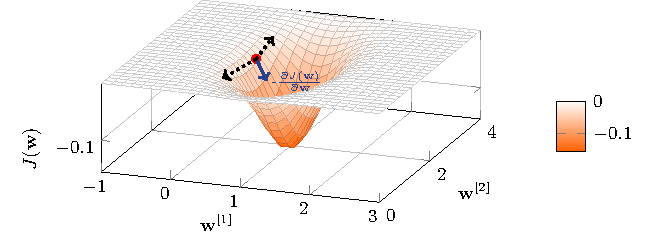
\includegraphics{./Chapter5/Figures/fig-gradient-descent.pdf}
\caption{函数上一个点沿着不同方向移动的示例}
\label{fig:5-43}
\end{figure}
%-------------------------------------------

\parinterval 应用梯度下降算法时,首先需要初始化参数$\mathbf{w}$。一般情况下深度学习中的参数应该初始化为一个不太大的随机数。一旦初始化$\mathbf{w}$后,就开始对模型进行不断的更新,{\small\sffamily\bfseries{参数更新的规则}}\index{参数更新的规则}(Update Rule)\index{Update Rule}为:
\begin{eqnarray}
\mathbf w_{t+1}&=&\mathbf w_{t}-\alpha \cdot \frac{\partial J(\mathbf w)}{\partial \mathbf w}
\label{eq:5-29}
\end{eqnarray}

\noindent 其中$t $表示更新的步数,$ \alpha $是一个超参数,被称作{\small\sffamily\bfseries{学习率}}\index{学习率}(Learning Rate)\index{Learning Rate},表示更新步幅的大小。$ \alpha $的设置需要根据任务进行调整。

\parinterval 从优化的角度看,梯度下降是一种典型的 {\small\bfnew{基于梯度的方法}}\index{基于梯度的方法}(Gradient-based Method)\index{Gradient-based Method},属于基于一阶导数的方法。其他类似的方法还有牛顿法、共轭方向法、拟牛顿法等。在具体实现时,公式\ref{eq:5-29}可以有以下不同的形式。\\

%----------------------------------------------------------------------------------------
%
%----------------------------------------------------------------------------------------

\vspace{0.5em}
\noindent {\small\sffamily\bfseries{批量梯度下降\index{批量梯度下降}(Batch Gradient Descent)\index{Batch Gradient Descent}}}
\vspace{0.5em}

\parinterval 批量梯度下降是梯度下降方法中最原始的形式,这种梯度下降方法在每一次迭代时使用所有的样本进行参数更新。参数优化的目标函数是
\begin{eqnarray}
J(\mathbf w)&=&\frac{1}{n}\sum_{i=1}^{n}{L(\mathbf x_i,\mathbf {\widetilde y}_i;\mathbf w)}
\label{eq:5-30}
\end{eqnarray}

\parinterval 式\ref{eq:5-30}是式\ref{eq:5-29}的严格实现,也就是将全部训练样本的平均损失作为目标函数。由全数据集确定的方向能够更好地代表样本总体,从而朝着模型在数据上整体优化所在的方向更新参数。

\parinterval 不过,这种方法的缺点也十分明显,因为要在全部训练数据上最小化损失,每一次参数更新都需要计算在所有样本上的损失。在使用海量数据进行训练的情况下,这种计算是非常消耗时间的。当训练数据规模很大时,很少使用这种方法。

%----------------------------------------------------------------------------------------
%
%----------------------------------------------------------------------------------------

\vspace{0.5em}
\noindent {\small\sffamily\bfseries{随机梯度下降\index{随机梯度下降}(Stochastic Gradient Descent)\index{Stochastic Gradient Descent}}}
\vspace{0.5em}

\parinterval 随机梯度下降(简称SGD)不同于批量梯度下降,每次迭代只使用一个样本对参数进行更新。SGD的目标函数是
\begin{eqnarray}
J(\mathbf w)&=&L(\mathbf x_i,\mathbf {\widetilde y}_i;\mathbf w)
\label{eq:5-31}
\end{eqnarray}

\noindent 由于每次只随机选取一个样本$(\mathbf x_i,\mathbf {\widetilde y}_i)$进行优化,这样更新的计算代价低,参数更新的速度大大加快,而且也适用于利用少量样本进行在线学习的情况\footnote{比如,训练数据不是一次给定的,而是随着模型的使用不断追加的。这时,需要不断地用新的训练样本更新模型,这种模式也被称作{\scriptsize\bfnew{在线学习}}(Online Learning)。}。

\parinterval 因为随机梯度下降算法每次优化的只是某一个样本上的损失,所以它的问题也非常明显:单个样本上的损失无法代表在全部样本上的损失,因此参数更新的效率低,方法收敛速度极慢。即使在目标函数为强凸函数的情况下,SGD仍旧无法做到线性收敛。

%----------------------------------------------------------------------------------------
%
%----------------------------------------------------------------------------------------

\vspace{0.5em}
\noindent {\small\sffamily\bfseries{小批量梯度下降\index{小批量梯度下降}(Mini-Batch Gradient Descent)\index{Mini-Batch Gradient Descent}}}
\vspace{0.5em}

\parinterval 为了综合批量梯度下降和随机梯度下降的优缺点,在实际应用中一般采用这两个算法的折中\ \dash \ 小批量梯度下降。其思想是:每次迭代计算一小部分训练数据的损失函数,并对参数进行更新。这一小部分数据被称为一个批次(mini-batch或者batch)。小批量梯度下降的参数优化的目标函数如下:
\begin{eqnarray}
J(\mathbf w)&=&\frac{1}{m}\sum_{i=j}^{j+m-1}{L(\mathbf x_i,\mathbf {\widetilde y}_i;\mathbf w)}
\label{eq:5-32}
\end{eqnarray}

\noindent 其中$ m $表示一个批次中的样本的数量,$ j $表示这个批次在全体训练数据的起始位置。这种方法可以更充分的利用GPU设备,因为批次中的样本可以一起计算。而且每次使用多个样本可以大大减小使模型收敛所需要的参数更新次数。但是需要注意的是批次大小的选择对模型的最终性能是存在一定影响的。

%----------------------------------------------------------------------------------------
%    NEW SUBSUB-SECTION
%----------------------------------------------------------------------------------------

\subsubsection{梯度获取}

\parinterval 梯度下降算法的一个核心是要得到目标函数相对于参数的梯度。下面将介绍三种常见的求梯度方法:数值微分、符号微分和自动微分,深度学习实现过程中多是采用自动微分方法计算梯度\cite{baydin2017automatic}。

%----------------------------------------------------------------------------------------
%
%----------------------------------------------------------------------------------------

\vspace{0.5em}
\noindent {\small\sffamily\bfseries{数值微分\index{数值微分}(Numerical Differentiation)\index{Numerical Differentiation}}}
\vspace{0.5em}

\parinterval 数学上,梯度的求解其实就是求函数偏导的问题。导数是用极限来定义的,如下:
\begin{eqnarray}
\frac{\partial L(\mathbf w)}{\partial \mathbf w}&=&\lim\limits_{\Delta \mathbf w \to 0}\frac{L(\mathbf w+\Delta \mathbf w)-L(\mathbf w-\Delta \mathbf w)}{2\Delta \mathbf w}
\label{eq:5-33}
\end{eqnarray}

\noindent 其中,$ \Delta \mathbf w $表示参数的一个很小的变化值。式\ref{eq:5-33}也被称作导数的双边定义。如果一个函数是初等函数,可以用求导法则来求得其导函数。如果不知道函数导数的解析式,则必须利用数值方法来求解该函数在某个点上的导数,这种方法就是数值微分。

\parinterval 数值微分根据导数的原始定义完成,根据公式可知,要得到损失函数在某个参数状态$ \mathbf w $下的梯度,可以将$ \mathbf w $增大或减小一点($ \Delta \mathbf w $),例如,取$ \Delta \mathbf w=0.0001 $,之后观测损失函数的变化与$ \Delta \mathbf w $的比值。$ \Delta \mathbf w $的取值越小计算的结果越接近导数的真实值,但是对计算的精度要求越高。

\parinterval 这种求梯度的方法很简单,但是计算量很大,求解速度非常慢,而且这种方法会造成{\small\sffamily\bfseries{截断误差}}\index{截断误差}(Truncation Error)\index{Truncation Error}和{\small\sffamily\bfseries{舍入误差}}\index{舍入误差}(Round-off Error)\index{Round-off Error}。在网络比较复杂、参数量稍微有点大的模型上一般不会使用这种方法。

\parinterval 截断误差和舍入误差是如何造成的呢?数值微分方法求梯度时,需用极限或无穷过程来求得。然而计算机需要将求解过程化为一系列有限的算术运算和逻辑运算。这样就要对某种无穷过程进行``截断'',即仅保留无穷过程的前段有限序列而舍弃它的后段。这就带来截断误差;舍入误差,是指运算得到的近似值和精确值之间的差异。由于数值微分方法计算复杂函数的梯度问题时,经过无数次的近似,每一次近似都产生了舍入误差,在这样的情况下,误差会随着运算次数增加而积累得很大,最终得出没有意义的运算结果。实际上,截断误差和舍入误差在训练复杂神经网络中,特别是使用低精度计算时,也会出现,因此是实际系统研发中需要注意的问题。

\parinterval 尽管数值微分不适用于大模型中的梯度求解,但是由于其非常简单,因此经常被用于检验其他梯度计算方法的正确性。比如在实现反向传播的时候(详见\ref{sec:5.4.6}节),可以检验求导是否正确(Gradient Check),这个过程就是利用数值微分实现的。\\ \\

%----------------------------------------------------------------------------------------
%
%----------------------------------------------------------------------------------------

\noindent {\small\sffamily\bfseries{ 符号微分\index{符号微分}(Symbolic Differentiation)\index{Symbolic Differentiation}}}
\vspace{0.5em}

\parinterval 顾名思义,符号微分就是通过建立符号表达式求解微分的方法:借助符号表达式和求导公式,推导出目标函数关于自变量的微分表达式,最后再带入具体数值得到微分结果。例如,对于表达式$ L(\mathbf w)=\mathbf x\cdot \mathbf w+2\mathbf w^2 $,可以手动推导出微分表达式$ \frac{\partial L(\mathbf w)}{\partial \mathbf w}=\mathbf x+4\mathbf w  $,最后将具体数值$ \mathbf x = {(\begin{array}{cc} 2 & -3\end{array})} $和$ \mathbf w = {(\begin{array}{cc} -1 & 1\end{array})} $带入后,得到微分结果$\frac{\partial L(\mathbf w)}{\partial \mathbf w}= {(\begin{array}{cc} 2 & -3\end{array})}+4{(\begin{array}{cc} -1 & 1\end{array})}= {(\begin{array}{cc} -2 & 1\end{array})}$。

\parinterval  使用这种求梯度的方法,要求必须将目标函数转化成一种完整的数学表达式,这个过程中存在{\small\bfnew{表达式膨胀}}\index{表达式膨胀}(Expression Swell)\index{Expression Swell}的问题,很容易导致符号微分求解的表达式急速``膨胀'',大大增加系统存储和处理表达式的负担。关于这个问题的一个实例请看表\ref{tab:5-4}。在深层的神经网络中,神经元数量和参数量极大,损失函数的表达式会非常冗长,不易存储和管理,而且,仅仅写出损失函数的微分表达式就是一个很庞大的工作量。从另一方面来说,这里真正需要的是微分的结果值,而不是微分表达式,推导微分表达式仅仅是求解过程中的中间产物。

%--------------------------------------------------------------------
\begin{table}[htp]
\centering
\caption{符号微分的表达式随函数的规模增加而膨胀}
\label{tab:5-4}
\small
\begin{tabular}{l | l l}
\rule{0pt}{18pt}     函数 & 微分表达式 & 化简的微分表达式  \\
\hline
\rule{0pt}{18pt}     $x$ & $1$ & $1$ \\
\rule{0pt}{18pt}     $x\cdot(x+1)$ & $(x+1)+x$ & $2x + 1$ \\
\rule{0pt}{18pt}     $x\cdot(x+1)\cdot$ & $(x+1)\cdot(x^2+x+1)$ & $4x^3+6x^2$ \\
$(x^2+x+1)$ & $+x\cdot(x^2+x+1)$ & $+4x+1$ \\
                     & $+x\cdot(x+1)\cdot(2x+1)$ & \\
\rule{0pt}{18pt}     $(x^2+x)\cdot$ & $(2x+1)\cdot(x^2+x+1)\cdot$ & $8x^7+28x^6$ \\
$(x^2+x+1)\cdot$ & $(x^4+2x^3+2x^2+x+1)$ & $+48x^5+50x^4$ \\
$(x^4+2x^3$ & $+(2x+1)\cdot(x^2+x)\cdot$ & $+36x^3+18x^2$ \\
$+2x^2+x+1)$ & \ \ $(x^4+2x^3+2x^2+x+1)$ & $+6x+1$ \\
 & $+(x^2+x)\cdot(x^2+x+1)\cdot$ & \\
 & \ \ $(4x^3+6x^2+4x+1)$ & \\
\end{tabular}
\end{table}
%--------------------------------------------------------------------

%----------------------------------------------------------------------------------------
%
%----------------------------------------------------------------------------------------

\vspace{0.5em}
\noindent {\small\sffamily\bfseries{自动微分\index{自动微分}(Automatic Differentiation)\index{Automatic Differentiation}}}
\vspace{0.5em}

\parinterval  自动微分是一种介于数值微分和符号微分的方法:将符号微分应用于最基本的算子,如常数、幂函数、指数函数、对数函数、三角函数等,然后代入数值,保留中间结果,最后再应用于整个函数。通过这种方式,将复杂的微分变成了简单的步骤,这些步骤完全自动化,而且容易进行存储和计算。

\parinterval  由于它只对基本函数或常数运用符号微分法则,所以它非常适合嵌入编程语言的循环条件等结构中,形成一种程序化的微分过程。在具体实现时,自动微分往往被当做是一种基于图的计算,相关的理论和技术方法相对成熟,因此是深度学习中使用最广泛的一种方法。不同于一般的编程模式,图计算先生成计算图,然后按照计算图执行计算过程。

\parinterval  自动微分可以用一种{\small\sffamily\bfseries{反向模式}}\index{反向模式}(Backward Mode)\index{Backward Mode}即反向传播思想进行描述。首先,从神经网络的输入,逐层计算每层网络的输出值。如图\ref{fig:5-44},第$ i $层的输出$ \mathbf h_i $作为第$ i+1 $层的输入,数据流在神经网络内部逐层传递。

%----------------------------------------------
\begin{figure}[htp]
\centering
%%%------------------------------------------------------------------------------------------------------------
\begin{tikzpicture}
\begin{scope}
\tikzstyle{layernode} = [draw,thick,fill=ugreen!30!white,blur shadow={shadow xshift=1pt,shadow yshift=-1pt}];

\node [anchor=center,layernode,minimum height=4em,minimum width=1em] (layer01) at (0,0) {};
\node [anchor=north west,layernode,minimum height=3em,minimum width=1em] (layer02) at ([xshift=3em]layer01.north east) {};
\node [anchor=south west,layernode,minimum height=3em,minimum width=1em] (layer03) at ([xshift=7em]layer01.south east) {};
\node [anchor=south west,layernode,minimum height=4em,minimum width=1em] (layer04) at ([xshift=11em]layer01.south east) {};
\node [anchor=south west,layernode,minimum height=4em,minimum width=1em] (layer05) at ([xshift=3em]layer04.south east) {};

\node [anchor=east] (input) at ([xshift=-1em]layer01.west){\scriptsize{输入}};
\node [anchor=west] (output) at ([xshift=1em]layer05.east){\scriptsize{输出}};


{
\draw [->,very thick,ublue] ([xshift=-1em]layer01.west) -- ([xshift=-0.1em]layer01.west)node [pos=0.5,above] {\small{\ding{172}}};;
}
{
\draw [->,very thick,ublue] ([xshift=0.1em,yshift=-0.5em]layer01.north east) -- ([xshift=-0.1em,yshift=-0.5em]layer02.north west)node [pos=0.5,above] {\small{\ding{173}}};
}
{
\draw [->,very thick,ublue] ([xshift=0.1em,yshift=0.5em]layer01.south east) -- ([xshift=-0.1em,yshift=0.5em]layer03.south west)node [pos=0.5,below] {\small{\ding{174}}};
}
{
\draw [->,very thick,ublue] ([xshift=0.1em,yshift=-0.5em]layer02.north east) -- ([xshift=-0.1em,yshift=-0.5em]layer04.north west)node [pos=0.5,above] {\small{\ding{175}}};
\draw [->,very thick,ublue] ([xshift=0.1em,yshift=0.5em]layer03.south east) -- ([xshift=-0.1em,yshift=0.5em]layer04.south west)node [pos=0.5,below] {\small{\ding{176}}};
\draw [->,very thick,ublue] ([xshift=0.1em]layer04.east) -- ([xshift=-0.1em]layer05.west)node [pos=0.5,above] {\small{\ding{177}}};
\draw [->,very thick,ublue] ([xshift=0.1em]layer05.east) -- ([xshift=1.0em]layer05.east)node [pos=0.5,above] {\small{\ding{178}}};
}



{
\draw [<-,thin] ([xshift=0.3em,yshift=0.3em]layer04.east) .. controls +(35:1) and +(215:1) .. ([xshift=-2em,yshift=0.3em]layer05.north west) node [pos=1,above] {\scriptsize{前向:层$i$ 的输出$h_{i}$}};
}


\end{scope}
\end{tikzpicture}
%%%------------------------------------------------------------------------------------------------------------


\caption{前向计算示意图}
\label{fig:5-44}
\end{figure}
%-------------------------------------------

\parinterval  前向计算实际上就是网络构建的过程,所有的计算都会被转化为计算图上的节点,前向计算和反向计算都依赖计算图来完成。构建计算图有以下两种实现方式:

\begin{itemize}
\vspace{0.5em}
\item 动态图(如Pytorch、NiuTensor等):前向计算与计算图的搭建同时进行,函数表达式写完即能得到前向计算的结果,有着灵活、易于调试的优点。
\vspace{0.5em}
\item 静态图(如Tensorflow):先搭建计算图,后执行运算,函数表达式完成后,并不能得到前向计算结果,需要显性调用一个Forward函数。但是计算图可以进行深度优化,执行效率较高。
\vspace{0.5em}
\end{itemize}

\parinterval  对于反向计算的实现,一般从神经网络的输出开始,逆向逐层计算每层网络输入所对应的微分结果。如图\ref{fig:5-45},在第$ i $层计算此处的梯度$ \frac{\partial L}{\partial \mathbf h_i} $,并将微分值向前一层传递,根据链式法则继续计算梯度。

%----------------------------------------------
\begin{figure}[htp]
\centering
%%%------------------------------------------------------------------------------------------------------------
\begin{tikzpicture}
\begin{scope}
\tikzstyle{layernode} = [draw,thick,fill=ugreen!30!white,blur shadow={shadow xshift=1pt,shadow yshift=-1pt}];

\node [anchor=center,layernode,minimum height=4em,minimum width=1em] (layer01) at (0,0) {};
\node [anchor=north west,layernode,minimum height=3em,minimum width=1em] (layer02) at ([xshift=3em]layer01.north east) {};
\node [anchor=south west,layernode,minimum height=3em,minimum width=1em] (layer03) at ([xshift=7em]layer01.south east) {};
\node [anchor=south west,layernode,minimum height=4em,minimum width=1em] (layer04) at ([xshift=11em]layer01.south east) {};
\node [anchor=south west,layernode,minimum height=4em,minimum width=1em] (layer05) at ([xshift=3em]layer04.south east) {};

\node [anchor=east] (input) at ([xshift=-1em]layer01.west){\scriptsize{输入}};
\node [anchor=west] (output) at ([xshift=1em]layer05.east){\scriptsize{输出}};
{
\draw [<-,very thick,red] ([xshift=-1em,yshift=-0.3em]layer01.west) -- ([xshift=-0.1em,yshift=-0.3em]layer01.west)node [pos=0.5,above] {\small{\ding{178}}};
\draw [<-,very thick,red] ([xshift=0.1em,yshift=-0.8em]layer01.north east) -- ([xshift=-0.1em,yshift=-0.8em]layer02.north west)node [pos=0.5,above] {\small{\ding{177}}};
\draw [<-,very thick,red] ([xshift=0.1em,yshift=0.2em]layer01.south east) -- ([xshift=-0.1em,yshift=0.2em]layer03.south west)node [pos=0.5,below] {\small{\ding{176}}};
\draw [<-,very thick,red] ([xshift=0.1em,yshift=-0.8em]layer02.north east) -- ([xshift=-0.1em,yshift=-0.8em]layer04.north west)node [pos=0.5,above] {\small{\ding{175}}};
\draw [<-,very thick,red] ([xshift=0.1em,yshift=0.2em]layer03.south east) -- ([xshift=-0.1em,yshift=0.2em]layer04.south west)node [pos=0.5,below] {\small{\ding{174}}};
\draw [<-,very thick,red] ([xshift=0.1em,yshift=-0.3em]layer04.east) -- ([xshift=-0.1em,yshift=-0.3em]layer05.west)node [pos=0.5,above] {\small{\ding{173}}};
\draw [<-,very thick,red] ([xshift=0.1em,yshift=-0.3em]layer05.east) -- ([xshift=1.0em,yshift=-0.3em]layer05.east)node [pos=0.5,above] {\small{\ding{172}}};
}


{
\draw [<-,thin] ([xshift=0.3em,yshift=-0.7em]layer04.east) .. controls +(-35:1) and +(145:1) .. ([xshift=-2em,yshift=-0.9em]layer05.south west) node [pos=1,below] {\scriptsize{反向:$h_{i}$ 处的梯度$\frac{\partial L}{\partial h_i}$}};
}

\end{scope}
\end{tikzpicture}
%%%------------------------------------------------------------------------------------------------------------


\caption{反向计算示意图}
\label{fig:5-45}
\end{figure}
%-------------------------------------------

\parinterval  反向计算也是深度学习中反向传播方法的基础。其实现的内部细节将在\ref{sec:5.4.6}节详细阐述,所以在这里不再赘述。

%----------------------------------------------------------------------------------------
%    NEW SUBSUB-SECTION
%----------------------------------------------------------------------------------------

\subsubsection{基于梯度的方法的变种和改进}\label{sec:5.4.2.3}

\parinterval  参数优化通常基于梯度下降算法,即在每个更新步骤$ t $,沿梯度方向更新参数:
\begin{eqnarray}
\mathbf w_{t+1}&=&\mathbf w_{t}-\alpha \cdot \frac{\partial J(\mathbf w_t)}{\partial \mathbf w_t}
\label{}
\end{eqnarray}

\noindent 其中$ \alpha $是一个超参数,表示更新步幅的大小,称作{\small\bfnew{学习率}}\index{学习率}(Learning Rate)\index{Learning Rate}。当然,这是一种最基本的梯度下降方法。如果函数的形状非均向,比如呈延伸状,搜索最优点的路径就会非常低效,因为这时梯度的方向并没有指向最小值的方向,并且随着参数的更新,梯度方向往往呈锯齿状,这将是一条相当低效的路径;此外这种梯度下降算法并不是总能到达最优点,而是在其附近徘徊;还有一个最令人苦恼的问题\ \dash \ 设置学习率,如果学习率设置的比较小,会导致训练收敛速度慢,如果学习率设置的比较大,会导致训练过程中因为优化幅度过大而频频跳过最优点。我们希望网络在优化的时候损失函数有一个很好的收敛速度同时又不至于摆动幅度太大。

\parinterval  针对以上问题,很多学者尝试对梯度下降方法做出改进,如Momentum, Adagrad, Adadelta, RMSprop, Adam, AdaMax, Nadam, AMSGrad等等,在这里将介绍Momentum、AdaGrad、RMSprop、Adam这4 种方法。

%----------------------------------------------
\begin{figure}[htp]
\centering

%%%------------------------------------------------------------------------------------------------------------
\begin{tikzpicture}
\begin{scope}


\node [anchor=center,color=red] (node1) at (0,0) {};
\node [anchor=north,color=red] (node4) at ([xshift=9.0em,yshift=0.88em]node1.south) {\large{$\bullet$}};
\node [anchor=north,color=red] (node5) at ([xshift=6.35em,yshift=-2.5em]node1.south) {\large{$\bullet$}};
\node [anchor=north,color=red] (node6) at ([xshift=3.8em,yshift=-0.5em]node1.south) {\large{$\bullet$}};
\node [anchor=north,color=red] (node7) at ([xshift=2.6em,yshift=-2.0em]node1.south) {\large{$\bullet$}};
\node [anchor=north,color=red] (node8) at ([xshift=1.22em,yshift=-0.91em]node1.south) {\large{$\bullet$}};
\node [anchor=north,color=red] (node9) at ([xshift=0.6em,yshift=-1.7em]node1.south) {\large{$\bullet$}};
\node [anchor=north,color=red] (node10) at ([xshift=0.0em,yshift=-1.2em]node1.south) {\large{$\bullet$}};

\draw[-,ublue,line width=0.3mm]([xshift=0.5em,yshift=0.46em]node4.south west)--([xshift=-0.5em,yshift=-0.4em]node5.north east);
\draw[-,ublue,line width=0.3mm]([xshift=-0.45em,yshift=0.52em]node6.south east)--([xshift=0.47em,yshift=-0.43em]node5.north west);
\draw[-,ublue,line width=0.3mm]([xshift=0.5em,yshift=0.46em]node6.south west)--([xshift=-0.5em,yshift=-0.4em]node7.north east);
\draw[-,ublue,line width=0.3mm]([xshift=-0.45em,yshift=0.52em]node8.south east)--([xshift=0.47em,yshift=-0.43em]node7.north west);
\draw[-,ublue]([xshift=0.5em,yshift=0.46em]node8.south west)--([xshift=-0.5em,yshift=-0.4em]node9.north east);
\draw[-,ublue,line width=0.3mm]([xshift=-0.78em,yshift=0.77em]node9.south east)--([xshift=0.78em,yshift=-0.68em]node10.north west);




\draw [-,ublue] (0,0) .. controls (2,0) and (3,-1.0)..(3,-1.5) .. controls (3,-2.2) and (2,-1.75)..(1.5,-1.65)..controls (1.5,-1.65) and (0.5,-1.45)..(0,-1.45)..controls (-0.5,-1.45) and (-1.5,-1.65)..(-1.5,-1.65)..controls (-2,-1.75)and (-3,-2.2).. (-3,-1.5)..controls (-3,-1.0) and (-2,0)..(0,0);

\draw [-,ublue] (0,0.5)..controls (2,0.5) and (4,-1.0).. (4,-1.7)..controls(4,-2.6)and (3,-2.3)..(2,-2.05)..controls (2,-2.05) and (1,-1.80)..(0,-1.80)..controls (-1,-1.80)and (-2,-2.05)..(-2,-2.05)..controls(-3,-2.3)and(-4,-2.6)..(-4,-1.7)..controls(-4,-1.0)and (-2,0.5)..(0,0.5);

\draw[-,ublue](0,1.0)..controls(3,1.0) and (5,-1.0)..(5,-1.9)..controls (5,-3.2)and (4,-2.7)..(3,-2.5)..controls (3,-2.5) and (2,-2.20)..(0,-2.15)..controls (-2,-2.20)and (-3,-2.5)..(-3,-2.5)..controls (-4,-2.7) and (-5,-3.2) ..(-5,-1.9)..controls (-5,-1.0) and (-3,1.0)..(0,1.0);

\draw[-,ublue] (0,-0.3)..controls (1.5,-0.3)and (2.5,-1.0)..(2.5,-1.4)..controls(2.5,-1.8)and (2,-1.55)..(1.5,-1.45) ..controls (1.5,-1.45) and (0.5,-1.25)..(0,-1.25) .. controls(-0.5,-1.25)and (-1.5,-1.45)..(-1.5,-1.45)..controls(-2,-1.55)and (-2.5,-1.8) ..(-2.5,-1.4)..controls(-2.5,-1.0) and (-1.5,-0.3)..(0,-0.3);

\draw[-,ublue](0,-0.5)..controls (1.0,-0.5) and (1.9,-0.8)..(1.9,-1.3)..controls(1.9,-1.5)and (1.5,-1.3)..(1.0,-1.2) ..controls(1.0,-1.2) and (0.5,-1.1)..(0,-1.1)..controls(-0.5,-1.1) and (-1.0,-1.2)..(-1.0,-1.2)..controls (-1.5,-1.3)and (-1.9,-1.5)..(-1.9,-1.3) ..controls(-1.9,-0.8)and (-1.0,-0.5) ..(0,-0.5);

\draw[-,ublue](0,-0.7)..controls(1.0,-0.7) and (1.4,-0.9)..(1.4,-1.1) .. controls(1.4,-1.25) and (1.2,-1.15)..(1.0,-1.1)..controls(1.0,-1.1) and (0.5,-0.95)..(0,-0.95)..controls(-0.5,-0.95)and (-1.0,-1.1) ..(-1.0,-1.1)..controls(-1.2,-1.15) and (-1.4,-1.25)..(-1.4,-1.1)..controls(-1.4,-0.9) and (-1.0,-0.7)..(0,-0.7);

\draw[-,ublue](0,-0.75)..controls(0.7,-0.75)and (1.0,-0.9)..(1.0,-1.0)..controls(1.0,-1.05) and (0.9,-1.05)..(0.7,-1.0)..controls(0.5,-0.95)and (0.3,-0.9)..(0,-0.9)..controls(-0.3,-0.9)and (-0.5,-0.95)..(-0.7,-1.0)..controls(-0.9,-1.05)and (-1.0,-1.05)..(-1.0,-1.0) ..controls(-1.0,-0.9)and (-0.7,-0.75)..(0,-0.75);

\draw[-,ublue](0,-0.8)..controls(0.5,-0.8) and (0.6,-0.85)..(0.6,-0.9)..controls(0.6,-0.93)and (0.5,-0.91)..(0.3,-0.88)..controls(0.2,-0.87)and (0.1,-0.86)..(0,-0.86)..controls(-0.1,-0.86)and(-0.2,-0.87)..(-0.3,-0.88)..controls(-0.5,-0.91) and(-0.6,-0.93) ..(-0.6,-0.9)..controls(-0.6,-0.85)and (-0.5,-0.8)..(0,-0.8);


\node [anchor=north] (labela) at (0,-2.7) {\footnotesize{(a)梯度下降算法中的``锯齿''现象}};

\end{scope}

%%%%%%%%%%%%%%%%%%%%%%%%%%%
\begin{scope}[yshift=-1.8in]


\node [anchor=center,color=red] (node1) at (0,0) {};

\node [anchor=north,color=red] (node2) at ([xshift=0.0em,yshift=-1.2em]node1.south) {\large{$\bullet$}};
\node [anchor=north,color=red] (node3) at ([xshift=3.55em,yshift=-0.981em]node1.south) {\large{$\bullet$}};
\node [anchor=north,color=red] (node4) at ([xshift=7.75em,yshift=-2.91em]node1.south) {\large{$\bullet$}};
\node [anchor=north,color=red] (node5) at ([xshift=11.38em,yshift=-1.11em]node1.south) {\large{$\bullet$}};

\draw[-,ublue,line width=0.3mm]([xshift=0.79em,yshift=-0.59em]node2.north west)--([xshift=-0.75em,yshift=0.6em]node3.south east);
\draw[-,ublue,line width=0.3mm]([xshift=0.79em,yshift=0.66em]node3.south west)--([xshift=-0.76em,yshift=-0.5em]node4.north east);
\draw[-,ublue,line width=0.3mm]([xshift=0.79em,yshift=-0.59em]node4.north west)--([xshift=-0.75em,yshift=0.6em]node5.south east);




\draw [-,ublue] (0,0) .. controls (2,0) and (3,-1.0)..(3,-1.5) .. controls (3,-2.2) and (2,-1.75)..(1.5,-1.65)..controls (1.5,-1.65) and (0.5,-1.45)..(0,-1.45)..controls (-0.5,-1.45) and (-1.5,-1.65)..(-1.5,-1.65)..controls (-2,-1.75)and (-3,-2.2).. (-3,-1.5)..controls (-3,-1.0) and (-2,0)..(0,0);

\draw [-,ublue] (0,0.5)..controls (2,0.5) and (4,-1.0).. (4,-1.7)..controls(4,-2.6)and (3,-2.3)..(2,-2.05)..controls (2,-2.05) and (1,-1.80)..(0,-1.80)..controls (-1,-1.80)and (-2,-2.05)..(-2,-2.05)..controls(-3,-2.3)and(-4,-2.6)..(-4,-1.7)..controls(-4,-1.0)and (-2,0.5)..(0,0.5);

\draw[-,ublue](0,1.0)..controls(3,1.0) and (5,-1.0)..(5,-1.9)..controls (5,-3.2)and (4,-2.7)..(3,-2.5)..controls (3,-2.5) and (2,-2.20)..(0,-2.15)..controls (-2,-2.20)and (-3,-2.5)..(-3,-2.5)..controls (-4,-2.7) and (-5,-3.2) ..(-5,-1.9)..controls (-5,-1.0) and (-3,1.0)..(0,1.0);

\draw[-,ublue] (0,-0.3)..controls (1.5,-0.3)and (2.5,-1.0)..(2.5,-1.4)..controls(2.5,-1.8)and (2,-1.55)..(1.5,-1.45) ..controls (1.5,-1.45) and (0.5,-1.25)..(0,-1.25) .. controls(-0.5,-1.25)and (-1.5,-1.45)..(-1.5,-1.45)..controls(-2,-1.55)and (-2.5,-1.8) ..(-2.5,-1.4)..controls(-2.5,-1.0) and (-1.5,-0.3)..(0,-0.3);

\draw[-,ublue](0,-0.5)..controls (1.0,-0.5) and (1.9,-0.8)..(1.9,-1.3)..controls(1.9,-1.5)and (1.5,-1.3)..(1.0,-1.2) ..controls(1.0,-1.2) and (0.5,-1.1)..(0,-1.1)..controls(-0.5,-1.1) and (-1.0,-1.2)..(-1.0,-1.2)..controls (-1.5,-1.3)and (-1.9,-1.5)..(-1.9,-1.3) ..controls(-1.9,-0.8)and (-1.0,-0.5) ..(0,-0.5);

\draw[-,ublue](0,-0.7)..controls(1.0,-0.7) and (1.4,-0.9)..(1.4,-1.1) .. controls(1.4,-1.25) and (1.2,-1.15)..(1.0,-1.1)..controls(1.0,-1.1) and (0.5,-0.95)..(0,-0.95)..controls(-0.5,-0.95)and (-1.0,-1.1) ..(-1.0,-1.1)..controls(-1.2,-1.15) and (-1.4,-1.25)..(-1.4,-1.1)..controls(-1.4,-0.9) and (-1.0,-0.7)..(0,-0.7);

\draw[-,ublue](0,-0.75)..controls(0.7,-0.75)and (1.0,-0.9)..(1.0,-1.0)..controls(1.0,-1.05) and (0.9,-1.05)..(0.7,-1.0)..controls(0.5,-0.95)and (0.3,-0.9)..(0,-0.9)..controls(-0.3,-0.9)and (-0.5,-0.95)..(-0.7,-1.0)..controls(-0.9,-1.05)and (-1.0,-1.05)..(-1.0,-1.0) ..controls(-1.0,-0.9)and (-0.7,-0.75)..(0,-0.75);

\draw[-,ublue](0,-0.8)..controls(0.5,-0.8) and (0.6,-0.85)..(0.6,-0.9)..controls(0.6,-0.93)and (0.5,-0.91)..(0.3,-0.88)..controls(0.2,-0.87)and (0.1,-0.86)..(0,-0.86)..controls(-0.1,-0.86)and(-0.2,-0.87)..(-0.3,-0.88)..controls(-0.5,-0.91) and(-0.6,-0.93) ..(-0.6,-0.9)..controls(-0.6,-0.85)and (-0.5,-0.8)..(0,-0.8);

\node [anchor=north] (labelb) at (0,-3) {\footnotesize{(b)Momentum梯度下降算法更加``平滑''地更新}};

\end{scope}
\end{tikzpicture}
%%%------------------------------------------------------------------------------------------------------------





\caption{Momentum梯度下降 vs 普通梯度下降}
\label{fig:5-46}
\end{figure}
%-------------------------------------------

%----------------------------------------------------------------------------------------
%
%----------------------------------------------------------------------------------------

\vspace{0.5em}
\noindent {\small\sffamily\bfseries{Momentum \index{Momentum}}}
\vspace{0.5em}

\parinterval  Momentum梯度下降算法的参数更新公式如下\footnote{在梯度下降算法的几种改进方法的公式中,其更新对象是某个具体参数而非参数矩阵,因此不再使用加粗样式}:
\begin{eqnarray}
v_t&=&\beta v_{t-1}+(1-\beta)\frac{\partial L}{\partial w_t}\label{eq:5-34}\\
w_{t+1}&=&w_t-\alpha v_t
\label{eq:5-35}
\end{eqnarray}

\parinterval  该算法引入了一个``动量''的理念\cite{qian1999momentum},它是基于梯度的移动指数加权平均。公式中的$ v_t $是损失函数在前$ t-1 $次更新中累积的梯度动量,$ \beta $是梯度累积的一个指数,这里一般设置值为0.9。所以Momentum梯度下降算法的主要思想就是对网络的参数进行平滑处理,让梯度的摆动幅度变得更小。

\parinterval  这里的``梯度''不再只是现在的损失函数的梯度,而是之前的梯度的加权和。在原始的梯度下降算法中,如果在某个参数状态下,梯度方向变化特别大,甚至与上一次参数更新中梯度方向成90度夹角,下一次参数更新中梯度方向可能又是一次90度的改变,这时参数优化路径将会成``锯齿''状(如图\ref{fig:5-46}所示),优化效率极慢。而Momentum梯度下降算法不会让梯度发生90度的变化,而是让梯度慢慢发生改变:如果当前的梯度方向与之前的梯度方向相同,在原梯度方向上加速更新参数;如果当前的梯度方向与之前的梯度方向相反,并不会产生一个急转弯,而是尽量把优化路径平滑地进行改变。这样做的优点也非常明显,一方面杜绝了``锯齿''状优化路径的出现,另一方面将优化幅度变得更加平滑,不会导致频频跳过最优点。

%----------------------------------------------------------------------------------------
%
%----------------------------------------------------------------------------------------

\vspace{0.5em}
\noindent {\small\sffamily\bfseries{AdaGrad \index{AdaGrad}}}
\vspace{0.5em}

\parinterval  在神经网络的学习中,学习率的设置很重要。学习率过小, 会导致学习花费过多时间;反过来,学习率过大,则会导致学习发散,甚至造成模型的``跑偏''。在深度学习实现过程中,有一种被称为学习率{\small\bfnew{衰减}}\index{衰减}(Decay)\index{Decay}的方法,即最初设置较大的学习率,随着学习的进行,使学习率逐渐减小,这种方法相当于将``全体''参数的学习率值一起降低。AdaGrad梯度下降算法进一步发展了这个思想\cite{duchi2011adaptive}。

\parinterval  AdaGrad会为参数的每个元素适当地调整学习率,与此同时进行学习。其参数更新公式为:
\begin{eqnarray}
z_t&=&z_{t-1}+\frac{\partial L}{\partial w_t} \cdot  \frac{\partial L}{\partial w_t}\label{eq:5-36}\\
w_{t+1}&=&w_t-\eta \frac{1}{\sqrt{z_t}}\cdot \frac{\partial L}{\partial w_t}
\label{eq:5-37}
\end{eqnarray}

\parinterval  这里新出现了变量$ z $,它保存了以前的所有梯度值的平方和,在更新参数时,通过乘以$ \frac{1}{\sqrt{z_t}} $ ,就可以调整学习的尺度。这意味着,变动较大(被大幅度更新)的参数的学习率将变小。也就是说,可以按参数的元素进行学习率衰减,使变动大的参数的学习率逐渐减小。

%----------------------------------------------------------------------------------------
%
%----------------------------------------------------------------------------------------

\vspace{0.5em}
\noindent {\small\sffamily\bfseries{RMSprop \index{RMSprop}}}
\vspace{0.5em}

\parinterval  RMSprop算法是一种自适应学习率的方法\cite{tieleman2012rmsprop},它是对AdaGrad算法的一种改进,可以避免AdaGrad算法中学习率不断单调下降以至于过早衰减的缺点。

\parinterval  RMSProp 算法沿袭了Momentum梯度下降算法中指数加权平均的思路,不过Momentum算法中加权平均的对象是梯度(即$ \frac{\partial L}{\partial w}$),而RMSProp 算法加权平均的对象是梯度的平方(即$ \frac{\partial L}{\partial w} \cdot  \frac{\partial L}{\partial w} $)。RMSProp 算法的参数更新公式为:
\begin{eqnarray}
z_t&=&\gamma z_{t-1}+(1-\gamma) \frac{\partial L}{\partial w_t} \cdot  \frac{\partial L}{\partial w_t}\label{eq:5-38}\\
w_{t+1}&=&w_t-\frac{\eta}{\sqrt{z_t+\epsilon}}\cdot \frac{\partial L}{\partial w_t}
\label{eq:5-39}
\end{eqnarray}

\parinterval  公式中的$ \epsilon $是为了维持数值稳定性而添加的常数,一版可设为 $ 10^{-8} $。和 AdaGrad 的想法类似,模型参数中每个元素都拥有各自的学习率。

\parinterval  RMSProp与AdaGrad相比,学习率的分母部分(即两种梯度下降算法迭代公式中的$ z $)的计算由累积方式变成了指数衰减移动平均。于是,每个参数的学习率并不是呈衰减趋势,而是既可以变小也可以变大,从而避免AdaGrad算法中学习率不断单调下降以至于过早衰减的缺点。

%----------------------------------------------------------------------------------------
%
%----------------------------------------------------------------------------------------

\vspace{0.5em}
\noindent {\small\sffamily\bfseries{Adam \index{Adam} }}
\vspace{0.5em}

\parinterval  Adam梯度下降算法是在RMSProp算法的基础上进行改进的,可以将其看成是带有动量项的RMSProp算法\cite{kingma2014adam}。该算法在自然语言处理领域非常流行。Adam 算法的参数更新公式如下,
\begin{eqnarray}
v_t&=&\beta v_{t-1}+(1-\beta)\frac{\partial L}{\partial w_t}\label{eq:5-40}\\
z_t&=&\gamma z_{t-1}+(1-\gamma) \frac{\partial L}{\partial w_t} \cdot  \frac{\partial L}{\partial w_t}\label{eq:5-41}\\
w_{t+1}&=&w_t-\frac{\eta}{\sqrt{z_t+\epsilon}} v_t
\label{eq:5-42}
\end{eqnarray}

\noindent 可以看到Adam 算法相当于在RMSProp算法中引入了Momentum算法中的动量项,这样做使得Adam算法兼具了Momentum算法和RMSProp算法的优点:既能使梯度更为``平滑''地更新,同时可以为神经网络中的每个参数设置不同的学习率。

\parinterval  需要注意的是包括Adam在内的很多参数更新算法中的学习率都需要人为设置。而且模型学习的效果与学习率的设置关系极大,甚至在研发实际系统时工程师需要进行大量的实验,才能得到最佳的模型。第六章还会具体介绍在机器翻译中参数更新学习率设置的策略。

%----------------------------------------------------------------------------------------
%    NEW SUB-SECTION
%----------------------------------------------------------------------------------------

\subsection{参数更新的并行化策略}

\parinterval  虽然通过GPU可以加速神经网络的运算,但当神经网络较为复杂时,模型训练还是需要几天甚至几周的时间。如果希望尽可能缩短一次学习所需的时间,最直接的想法就是把不同的训练样本分配给多个GPU 或CPU,然后在这些设备上同时进行训练,即实现并行化训练。这种方法也被称作{\small\sffamily\bfseries{数据并行}}\index{数据并行}。具体实现时,有两种常用的并行化策略:(参数)同步更新和(参数)异步更新。

\begin{itemize}
\vspace{0.5em}
\item {\small\sffamily\bfseries{同步更新}}\index{同步更新}(Synchronous Update)\index{Synchronous Update}是指所有计算设备完成计算后,统一汇总并更新参数。当所有设备的反向传播算法完成之后同步更新参数,不会出现单个设备单独对参数进行更新的情况。这种方法效果稳定,但是效率比较低,在同步更新时,每一次参数更新都需要所有设备统一开始、统一结束,如果设备的运行速度不一致,那么每一次参数更新都需要等待最慢的设备结束才能开始。
\vspace{0.5em}
\item {\small\sffamily\bfseries{异步更新}}\index{异步更新}(Asynchronous Update)\index{Asynchronous Update}是指每个计算设备可以随时更新参数。不同设备可以随时读取参数的最新值,然后根据当前参数值和分配的训练样本,各自执行反向传播过程并独立更新参数。由于设备间不需要相互等待,这种方法并行度高。但是不同设备读取参数的时间可能不同,会造成不同设备上的参数不同步,导致这种方法不十分稳定,有可能无法达到较好的训练结果。
\vspace{0.5em}
\end{itemize}

%----------------------------------------------
\begin{figure}[htp]
\centering
%%%------------------------------------------------------------------------------------------------------------
\begin{tikzpicture}

%%%%%%%%%%%%%%%%
% parameter server + processor
\begin{scope}[]

{\scriptsize

\tikzstyle{parametershard} = [draw,thick,minimum width=4em,align=left,rounded corners=2pt]

{
\node[parametershard,anchor=west,fill=yellow!10] (param1) at (0,0) {$W_o$};
\node (param2) at ([xshift=1em]param1.east) {};
\node[parametershard,anchor=west,fill=red!10] (param3) at ([xshift=1em]param2.east) {$W_h$};
\node[anchor=south,inner sep=1pt] (serverlabel) at ([yshift=0.2em]param2.north) {\footnotesize{\textbf{parameter server}: $\mathbf w_{new} = \mathbf w - \alpha\cdot \frac{\partial L}{\partial \mathbf w}$}};
}

\begin{pgfonlayer}{background}
{
\node[rectangle,draw,thick,inner sep=2pt,fill=gray!20] [fit = (param1) (param2) (param3) (serverlabel)] (serverbox) {};
}
\end{pgfonlayer}

\tikzstyle{processor} = [draw,thick,fill=orange!20,minimum width=4em,align=left,rounded corners=2pt]

{
\node [processor,anchor=north,align=center] (processor2) at ([yshift=-1.2in]serverlabel.south) {\scriptsize{Processor 2}\\\scriptsize{on GPU2 (G2)}};
\node [anchor=north] (labela) at ([xshift=4em,yshift=-1em]processor2.south) {\footnotesize {(a)同步更新}};
\node [processor,anchor=east,align=center] (processor1) at ([xshift=-1em]processor2.west) {\scriptsize{Processor 1}\\\scriptsize{on GPU1 (G1)}};
\node [processor,anchor=west,align=center] (processor3) at ([xshift=1em]processor2.east) {\scriptsize{Processor 3}\\\scriptsize{on GPU3 (G3)}};
}

{
\draw[->,very thick,red] ([xshift=-0.5em,yshift=2pt]processor2.north) -- ([xshift=-0.5em,yshift=-2pt]serverbox.south) node [pos=0.5,align=right,xshift=-2em] (pushlabel) {\scriptsize{$\frac{\partial L}{\partial \mathbf w}$}};;
\draw[<-,very thick,blue] ([xshift=0.5em,yshift=2pt]processor2.north) -- ([xshift=0.5em,yshift=-2pt]serverbox.south) node [pos=0.5,align=left,xshift=2.2em] (fetchlabel) {\scriptsize{$\mathbf w_{new}$}};;;
\draw[->,very thick,red] ([xshift=-0.5em,yshift=2pt]processor3.north) --
 ([xshift=3em,yshift=-2pt]serverbox.south);
\draw[<-,very thick,blue] ([xshift=0.5em,yshift=2pt]processor3.north) -- ([xshift=4em,yshift=-2pt]serverbox.south) node [pos=0.5,align=left,xshift=2.2em] (fetchlabel) {\scriptsize{fetch (F)}};
\draw[->,very thick,red] ([xshift=-0.5em,yshift=2pt]processor1.north) -- ([xshift=-4em,yshift=-2pt]serverbox.south) node [pos=0.5,align=right,xshift=-2em] (pushlabel) {\scriptsize{push (P)}};
\draw[<-,very thick,blue] ([xshift=0.5em,yshift=2pt]processor1.north) -- ([xshift=-3em,yshift=-2pt]serverbox.south);
}

%%%%%%%%%%%
% synchronous mode
\tikzstyle{job} = [draw,rotate=90,minimum height=0.25in]

\scriptsize{
{
\node[job,anchor=south west,fill=blue!50] (fetch11) at ([xshift=6em,yshift=1em]processor3.east) {\textbf{F}};
\node[job,anchor=west,fill=orange!30] (minibatch11) at ([yshift=1pt]fetch11.east) {\tiny{minibatch3}};
\node[job,anchor=west,fill=red!50] (push11) at ([yshift=1pt]minibatch11.east) {\textbf{P}};
\node[job,anchor=north west,fill=blue!50] (fetch12) at ([xshift=0.8em]fetch11.south west) {\textbf{F}};
\node[job,anchor=west,fill=orange!30] (minibatch12) at ([yshift=1pt]fetch12.east) {\tiny{minibatch2}};
\node[job,anchor=west,fill=red!50] (push12) at ([yshift=1pt]minibatch12.east) {\textbf{P}};
\node[job,anchor=north west,fill=blue!50] (fetch13) at ([xshift=0.8em]fetch12.south west) {\textbf{F}};
\node[job,anchor=west,fill=orange!30,minimum width=8em] (minibatch13) at ([yshift=1pt]fetch13.east) {\scriptsize{minibatch1}};
\node[job,anchor=west,fill=red!50] (push13) at ([yshift=1pt]minibatch13.east) {\textbf{P}};
\node[anchor=south west,draw,fill=gray!20,minimum width=8.0em] (update11) at ([yshift=4.0em]push11.north east) {Update};

\node[anchor=north] (G11) at (fetch11.west) {\small{G3}};
\node[anchor=north] (G12) at (fetch12.west) {\small{G2}};
\node[anchor=north] (G13) at (fetch13.west) {\small{G1}};
\node[anchor=north,align=center] (synlabel) at (G12.south) {\small{\textbf{Synchronous}}\\\small{\textbf{Training}}};
\draw[->,thick] ([xshift=1em]G13.east) -- ([xshift=1em,yshift=1.4in]G13.east) node [pos=0.5,rotate=90,yshift=-1em] {\small{time line}};
}
}

{
\draw [<->,thin,dotted] ([xshift=-1pt]minibatch11.north) .. controls +(west:3em) and +(east:3em) .. ([xshift=1pt]processor3.east);
\draw [<->,thin,dotted] ([xshift=-1pt]fetch11.north) .. controls +(west:4em) and +(east:4em) .. ([xshift=-0.5em,yshift=0.3in]processor3.north);
\draw [<->,thin,dotted] ([xshift=-1pt]push11.north) -- ([xshift=-4em,yshift=0.8in]processor3.north);
}

{
\draw [<->,thin,dotted] ([xshift=-1pt]update11.west) -- ([xshift=1pt,yshift=-1.5em]serverbox.north east);
}


}

\end{scope}

\begin{scope}[yshift=-2.5in]

{\scriptsize

\tikzstyle{parametershard} = [draw,thick,minimum width=4em,align=left,rounded corners=2pt]

{
\node[parametershard,anchor=west,fill=yellow!10] (param1) at (0,0) {$W_o$};
\node (param2) at ([xshift=1em]param1.east) {};
\node[parametershard,anchor=west,fill=red!10] (param3) at ([xshift=1em]param2.east) {$W_h$};
\node[anchor=south,inner sep=1pt] (serverlabel) at ([yshift=0.2em]param2.north) {\footnotesize{\textbf{parameter server}: $\mathbf w_{new} = \mathbf w - \alpha\cdot \frac{\partial L}{\partial \mathbf w}$}};
}

\begin{pgfonlayer}{background}
{
\node[rectangle,draw,thick,inner sep=2pt,fill=gray!20] [fit = (param1) (param2) (param3) (serverlabel)] (serverbox) {};
}
\end{pgfonlayer}

\tikzstyle{processor} = [draw,thick,fill=orange!20,minimum width=4em,align=left,rounded corners=2pt]

{
\node [processor,anchor=north,align=center] (processor2) at ([yshift=-1.2in]serverlabel.south) {\scriptsize{Processor 2}\\\scriptsize{on GPU2 (G2)}};
\node [anchor=north] (label) at ([xshift=4em,yshift=-1em]processor2.south) {\footnotesize {(b)异步更新}};
\node [processor,anchor=east,align=center] (processor1) at ([xshift=-1em]processor2.west) {\scriptsize{Processor 1}\\\scriptsize{on GPU1 (G1)}};
\node [processor,anchor=west,align=center] (processor3) at ([xshift=1em]processor2.east) {\scriptsize{Processor 3}\\\scriptsize{on GPU3 (G3)}};
}

{
\draw[->,very thick,red] ([xshift=-0.5em,yshift=2pt]processor2.north) -- ([xshift=-0.5em,yshift=-2pt]serverbox.south) node [pos=0.5,align=right,xshift=-2em] (pushlabel) {\scriptsize{$\frac{\partial L}{\partial \mathbf w}$}};;
\draw[<-,very thick,blue] ([xshift=0.5em,yshift=2pt]processor2.north) -- ([xshift=0.5em,yshift=-2pt]serverbox.south) node [pos=0.5,align=left,xshift=2.2em] (fetchlabel) {\scriptsize{$\mathbf w_{new}$}};;;
\draw[->,very thick,red] ([xshift=-0.5em,yshift=2pt]processor3.north) --
 ([xshift=3em,yshift=-2pt]serverbox.south);
\draw[<-,very thick,blue] ([xshift=0.5em,yshift=2pt]processor3.north) -- ([xshift=4em,yshift=-2pt]serverbox.south) node [pos=0.5,align=left,xshift=2.2em] (fetchlabel) {\scriptsize{fetch (F)}};
\draw[->,very thick,red] ([xshift=-0.5em,yshift=2pt]processor1.north) -- ([xshift=-4em,yshift=-2pt]serverbox.south) node [pos=0.5,align=right,xshift=-2em] (pushlabel) {\scriptsize{push (P)}};
\draw[<-,very thick,blue] ([xshift=0.5em,yshift=2pt]processor1.north) -- ([xshift=-3em,yshift=-2pt]serverbox.south);
}

%%%%%%%%%%%
% synchronous mode
\tikzstyle{job} = [draw,rotate=90,minimum height=0.25in]

\scriptsize{
{
\node[job,anchor=south west,fill=blue!50] (fetch21) at ([xshift=6em,yshift=1em]processor3.east) {\textbf{F}};
\node[job,anchor=west,fill=orange!30] (minibatch21) at ([yshift=1pt]fetch21.east) {\tiny{minibatch3}};
\node[job,anchor=west,fill=red!50] (push21) at ([yshift=1pt]minibatch21.east) {\textbf{P}};
\node[job,anchor=north west,fill=blue!50] (fetch22) at ([xshift=0.8em]fetch21.south west) {\textbf{F}};
\node[job,anchor=west,fill=orange!30] (minibatch22) at ([yshift=1pt]fetch22.east) {\tiny{minibatch2}};
\node[job,anchor=west,fill=red!50] (push22) at ([yshift=1pt]minibatch22.east) {\textbf{P}};
\node[job,anchor=north west,fill=blue!50] (fetch23) at ([xshift=0.8em]fetch22.south west) {\textbf{F}};
\node[job,anchor=west,fill=orange!30,minimum width=8em] (minibatch23) at ([yshift=1pt]fetch23.east) {\scriptsize{minibatch1}};
\node[job,anchor=west,fill=red!50] (push23) at ([yshift=1pt]minibatch23.east) {\textbf{P}};
\node[anchor=south west,draw,fill=gray!20,minimum width=0.59in] (update21) at ([yshift=2pt]push21.north east) {Update};
\node[anchor=south west,draw,fill=gray!20,minimum width=0.25in] (update22) at ([yshift=2pt]push23.north east) {\tiny{Upd.}};

\node[anchor=north] (G21) at (fetch21.west) {\small{G3}};
\node[anchor=north] (G22) at (fetch22.west) {\small{G2}};
\node[anchor=north] (G23) at (fetch23.west) {\small{G1}};
\node[anchor=north,align=center] (synlabel) at (G22.south) {\small{\textbf{Asynchronous}}\\\small{\textbf{Training}}};
\draw[->,thick] ([xshift=1em]G23.east) -- ([xshift=1em,yshift=1.4in]G23.east) node [pos=0.5,rotate=90,yshift=-1em] {\small{time line}};

\draw [<->,thin,dotted] ([xshift=-1pt]update21.west) -- ([xshift=1pt,yshift=-1.5em]serverbox.north east);
\draw [<->,thin,dotted] ([xshift=-1pt]update22.west) -- ([xshift=1pt,yshift=-1.5em]serverbox.north east);
}
}

}

\end{scope}

\end{tikzpicture}
%%%------------------------------------------------------------------------------------------------------------





\caption{同步更新与异步更新对比}
\label{fig:5-47}
\end {figure}
%-------------------------------------------

\parinterval  图\ref{fig:5-47}对比了同步更新和异步更新的区别,在这个例子中,使用4台设备对一个两层神经网络中的参数进行更新,其中使用了一个{\small\bfnew{参数服务器}}\index{参数服务器}(Parameter Server\index{Parameter Server})来保存最新的参数,不同设备(Worker,图中的G1、G2、G3)可以通过同步或者异步的方式访问参数服务器。图中的$ \mathbf w_o $和$ \mathbf w_h $分别代表输出层和隐藏层的全部参数,操作push(P) 表示设备向参数服务器传送梯度,操作fetch(F)表示参数服务器向设备传送更新后的参数。

\parinterval  此外,在使用多个设备进行并行训练的时候,由于设备间带宽的限制,大量的数据传输会有较高的延时。对于复杂神经网络来说,设备间参数和梯度传递的时间消耗也会成为一个不得不考虑的因素。有时候,设备间数据传输的时间甚至比模型计算的时间都长,大大降低了并行度\cite{xiao2017fast}。对于这种问题,可以考虑对数据进行压缩或者减少传输的次数来缓解问题。

%----------------------------------------------------------------------------------------
%    NEW SUB-SECTION
%----------------------------------------------------------------------------------------

\subsection{梯度消失、梯度爆炸和稳定性训练}\label{sec:5.4.4}

\parinterval  深度学习中随着神经网络层数的增加,导数可能会出现指数级的下降或者指数级的增加,这种现象分别称为{\small\sffamily\bfseries{梯度消失}}\index{梯度消失}(Gradient Vanishing)\index{Gradient Vanishing}和{\small\sffamily\bfseries{梯度爆炸}}\index{梯度爆炸}(Gradient Explosion)\index{Gradient Explosion}。出现这两种现象的本质原因是反向传播过程中链式法则导致梯度矩阵的多次相乘。这类问题很容易导致训练的不稳定。

%----------------------------------------------------------------------------------------
%    NEW SUBSUB-SECTION
%----------------------------------------------------------------------------------------

\subsubsection{易于优化的激活函数}

\parinterval  网络训练过程中,如果每层网络的梯度都小于1,各层梯度的偏导数会与后面层传递而来的梯度相乘得到本层的梯度,并向前一层传递。该过程循环进行,最后导致梯度指数级地减小,这就产生了梯度消失现象。这种情况会导致神经网络层数较浅的部分梯度接近0。一般来说,产生很小梯度的原因是使用了类似于Sigmoid这样的激活函数,当输入的值过大或者过小的时候这类函数曲线会趋于直线,梯度近似为零。针对这个问题,主要的解决办法是使用更加易于优化的激活函数,比如,使用ReLU代替Sigmoid和Tanh作为激活函数。

\parinterval  缓解梯度消失问题最直接的想法就是希望各层的偏导数大于或等于1。图\ref{fig:5-48}展示了Sigmoid激活函数$ y=\frac{1}{1+e^{-x}}$的函数曲线和导函数曲线,如果使用Sigmoid作为损失函数,其梯度不可能超过0.25,这样经过链式求导之后,很容易发生梯度消失。

%----------------------------------------------
\begin{figure}[htp]
\centering
%%%------------------------------------------------------------------------------------------------------------
\begin{tikzpicture}
\begin{axis}[  
  name=sigmoid,
  width=6cm, height=4.5cm, 
  xtick={-5,-2.5,...,6},
  ytick={0,0.5,1.0},
  xlabel={$x$},
  ylabel={$y$},
  xlabel style={xshift=2.4cm,yshift=0.7cm},
  axis y line=middle,%y轴居中
  ylabel style={xshift=0.1cm,yshift=0cm},
  x axis line style={->},%x轴箭头
  axis line style={very thick},
  axis x line*=bottom,%将上面的x轴去掉,仅保留下面的x轴
  xmin=-6,
  xmax=6,
  ymin=0,
  ymax=1.4]
\addplot[draw=red,very thick]{1/(1 + exp( -x))};
\end{axis}
\node [anchor=north] (labelc) at (2.3,-0.5) {\footnotesize{(a)}};
\begin{axis}[
  at={(sigmoid.east)},
  anchor=east, 
  xshift=6cm,
  yshift=0cm,  
  width=6cm, height=4.5cm, 
  xtick={-4,-2,...,4},
  ytick={0,0.1,0.2},
  xlabel={$x$},
  ylabel={$y$},
  xlabel style={xshift=2.4cm,yshift=0.7cm},
  axis y line=middle,%y轴居中
  ylabel style={xshift=0.1cm,yshift=0cm},
  x axis line style={->},%x轴箭头
  axis line style={very thick},
  axis x line*=bottom,%将上面的x轴去掉,仅保留下面的x轴
  xmin=-6,
  xmax=6,
  ymin=0,
  ymax=0.3]
\addplot[draw=ublue,very thick]{(1/(1 + exp( -x)))*(1-(1/(1 + exp( -x))))};
\end{axis}
\node [anchor=north] (labelc) at (8.2,-0.5) {\footnotesize{(b)}};
\end{tikzpicture}
%%%------------------------------------------------------------------------------------------------------------


\caption{Sigmoid激活函数的函数曲线和导函数曲线}
\label{fig:5-48}
\end {figure}
%-------------------------------------------

\parinterval  同理,Tanh作为激活函数也容易出现梯度消失现象,图\ref{fig:5-49}展示了Tanh激活函数$ y=\frac{e^x-e^{-x}}{e^x+e^{-x}}$的函数曲线和导函数曲线,可以看出,Tanh激活函数比Sigmoid激活函数要好一些,但是Tanh激活函数的导数也小于1,因此无法避免梯度消失现象。

%----------------------------------------------
\begin{figure}[htp]
\centering
%%%------------------------------------------------------------------------------------------------------------
\begin{tikzpicture}
\begin{axis}[  
  name=tanh,
  width=6cm, height=4.5cm, 
  xtick={-5,-2.5,...,6},
  ytick={-1.0,-0.5,0,0.5,1.0},
  xlabel={$x$},
  ylabel={$y$},
  xlabel style={xshift=2.4cm,yshift=2.5cm},
  axis y line=middle,%y轴居中
  ylabel style={xshift=0.1cm,yshift=0cm},
  x axis line style={->},%x轴箭头
  axis line style={very thick},
  axis x line*=middle,%将上面的x轴去掉,仅保留下面的x轴
  xmin=-6,
  xmax=6,
  ymin=-1.2,
  ymax=1.2]
\addplot[draw=red,very thick]{tanh(x)};
\end{axis}
\node [anchor=north] (labelc) at (2.3,-0.5) {\footnotesize{(a)}};
\begin{axis}[  
  at={(tanh.east)},
  anchor=east, 
  xshift=6cm,
  yshift=0cm, 
  width=6cm, height=4.5cm, 
  xtick={-10,-5,...,10},
  ytick={0,0.5,1},
  xlabel={$x$},
  ylabel={$y$},
  xlabel style={xshift=2.4cm,yshift=0.7cm},
  axis y line=middle,%y轴居中
  ylabel style={xshift=0.1cm,yshift=0cm},
  x axis line style={->},%x轴箭头
  axis line style={very thick},
  axis x line*=bottom,%将上面的x轴去掉,仅保留下面的x轴
  xmin=-10,
  xmax=10,
  ymin=0,
  ymax=1.2]
\addplot[draw=ublue,very thick]{1-tanh(x)*tanh(x)};
\end{axis}
\node [anchor=north] (labelc) at (8.2,-0.5) {\footnotesize{(b)}};
\end{tikzpicture}
%%%------------------------------------------------------------------------------------------------------------


\caption{Tanh激活函数的函数曲线和导函数曲线}
\label{fig:5-49}
\end {figure}
%-------------------------------------------

\parinterval  ReLU激活函数的思想也很简单,如果激活函数的导数为1,那么就不存在梯度消失爆炸的问题了。图\ref{fig:5-50}展示了ReLU激活函数$ y={\rm{max}}(0,x)$的函数曲线和导函数曲线。可以很容易看出,ReLU函数的导数在正数部分是恒等于1的,因此在深层网络中使用ReLU激活函数就不会产生很小的梯度。

%----------------------------------------------
\begin{figure}[htp]
\centering
%%%------------------------------------------------------------------------------------------------------------
\begin{tikzpicture}
\begin{axis}[  
  name=relu,
  width=6cm, height=4.5cm, 
  xtick={-1.0,-0.5,...,1.0},
  ytick={0.5,1.0},
  xlabel={$x$},
  ylabel={$y$},
  xlabel style={xshift=2.4cm,yshift=0.7cm},
  axis y line=middle,%y轴居中
  ylabel style={xshift=0.1cm,yshift=0cm},
  x axis line style={->},%x轴箭头
  axis line style={very thick},
  axis x line*=middle,%将上面的x轴去掉,仅保留下面的x轴
  xmin=-1.2,
  xmax=1.2,
  ymin=0,
  ymax=1.2]
\addplot[domain=-1:0,draw=red,very thick]{0};
\addplot[domain=0:1,draw=red,very thick]{x};
\end{axis}
\node [anchor=north] (labelc) at (2.3,-0.5) {\footnotesize{(a)}};
\begin{axis}[  
  at={(relu.east)},
  anchor=east, 
  xshift=6cm,
  yshift=0cm, 
  width=6cm, height=4.5cm, 
  xtick={-4,-2,...,4},
  ytick={0,0.2,...,1.0},
  xlabel={$x$},
  ylabel={$y$},
  xlabel style={xshift=2.4cm,yshift=0.7cm},
  axis y line=middle,%y轴居中
  ylabel style={xshift=0.1cm,yshift=0cm},
  x axis line style={->},%x轴箭头
  axis line style={very thick},
  axis x line*=middle,%将上面的x轴去掉,仅保留下面的x轴
  xmin=-5,
  xmax=5,
  ymin=0,
  ymax=1.2]
\addplot[domain=-4:0,draw=ublue,very thick]{0};
\addplot[domain=0:4,draw=ublue,very thick]{1};
\end{axis}
\node [anchor=north] (labelc) at (8.2,-0.5) {\footnotesize{(b)}};
\end{tikzpicture}
%%%------------------------------------------------------------------------------------------------------------


\caption{ReLU激活函数的函数曲线和导函数曲线}
\label{fig:5-50}
\end {figure}
%-------------------------------------------

\parinterval  当然,梯度消失并不是仅仅可以通过改变激活函数就可以完全消除掉。随着网络层数的增加,很多因素都可能会造成梯度消失。后面也会进一步介绍其他手段,可以综合运用这些方法达到很好的缓解梯度消失问题的目的。

%----------------------------------------------------------------------------------------
%    NEW SUBSUB-SECTION
%----------------------------------------------------------------------------------------

\subsubsection{梯度裁剪}

\parinterval  网络训练过程中,如果参数的初始值过大,而且每层网络的梯度都大于1,反向传播过程中,各层梯度的偏导数都会比较大,会导致梯度指数级地增长直至超出浮点数表示的范围,这就产生了梯度爆炸现象。如果发生这种情况,模型中离输入近的部分比离输入远的部分参数更新得更快,使网络变得非常不稳定。在极端情况下,模型的参数值变得非常大,甚至于溢出。针对梯度爆炸的问题,常用的解决办法为{\small\sffamily\bfseries{梯度裁剪}}\index{梯度裁剪}(Gradient Clipping)\index{Gradient Clipping}。

\parinterval    梯度裁剪的思想是设置一个梯度剪切阈值。在更新梯度的时候,如果梯度超过这个阈值,就将其强制限制在这个范围之内。假设梯度为$ \mathbf g $,梯度剪切阈值为$ \theta $,梯\\ \\度裁剪的公式为
\begin{eqnarray}
\mathbf g&=&{\rm{min}}(\frac{\theta}{\Vert \mathbf g\Vert},1)\mathbf g
\label{eq:5-43}
\end{eqnarray}

\noindent 其中,$ \Vert \cdot \Vert $表示$ l_2 $范数。梯度裁剪经常被使用在层数较多的模型中,如循环神经网络。

%----------------------------------------------------------------------------------------
%    NEW SUBSUB-SECTION
%----------------------------------------------------------------------------------------

\subsubsection{稳定性训练}

\parinterval  为了使神经网络模型训练更加稳定,通常还会考虑其他策略。

\parinterval  (1){\small\bfnew{批量归一化}}\index{批量归一化}(Batch Normalization)\index{Batch Normalization}

\parinterval  批量归一化,顾名思义,是以进行学习时的小批量样本为单位进行归一化\cite{ioffe2015batch}。具体而言,就是对神经网络隐层输出的每一个维度,沿着批次的方向进行均值为0、方差为1的归一化。在深层神经网络中,每一层网络都可以使用批量归一化操作。这样使神经网络任意一层的输入不至于过大或过小,从而防止隐层中异常值导致模型状态的巨大改变。

\parinterval  (2){\small\bfnew{层归一化}}\index{层归一化}(Layer Normalization)\index{Layer Normalization}

\parinterval  类似的,层归一化更多是针对自然语言处理这种序列处理任务\cite{Ba2016LayerN},它和批量归一化的原理是一样的,只是归一化操作是在序列上同一层网络的输出结果上进行的,也就是归一化操作沿着序列方向进行。这种方法可以很好的避免序列上不同位置神经网络输出结果的不可比性。同时由于归一化后所有的结果都转化到一个可比的范围,使得隐层状态可以在不同层之间进行自由组合。

\parinterval  (3){\small\bfnew{残差网络}}\index{残差网络}(Residual Networks)\index{Residual Networks}

\parinterval  最初,残差网络是为了解决神经网络持续加深时的模型退化问题\cite{DBLP:journals/corr/HeZRS15},但是残差结构对解决梯度消失和梯度爆炸问题也有所帮助。有了残差结构,可以很轻松的构建几十甚至上百层的神经网络,而不用担心层数过深造成的梯度消失问题。残差网络的结构如图\ref{fig:5-51}所示:

%----------------------------------------------
\begin{figure}[htp]
\centering
%%%------------------------------------------------------------------------------------------------------------
\begin{tikzpicture}
\begin{scope}


\node [anchor=center] (node6) at (0,0) {};
\node[anchor=west](node6-1) at ([xshift=-0.2em,yshift=-0.6em]node6.east) {\footnotesize{$\rm{ReLU}$}};
\node [anchor=north](node3)at ([yshift=-1.2em]node6.south){$\bigoplus$};
\draw[->,thick]([yshift=-0.32em]node3.north)--(node6.south);

\node [anchor=north,draw,thick](node2)at ([yshift=-1.2em]node3.south){\small{weight layer}};
\draw[->,thick](node2.north)--([yshift=0.35em]node3.south);
\node[anchor=west](node2-1) at ([xshift=2.1em,yshift=1.2em]node2.east) {$\mathbf{x}$};
\node[anchor=north](node2-2) at ([xshift=0.2em,yshift=-0.3em]node2-1.south) {\footnotesize{$\rm{identity}$}};

\node [anchor=east](node4) at ([xshift=-0.2em]node2.west) {$\textrm{F}(\mathbf{x})$};
\node [anchor=east](node5) at ([xshift=-0.3em]node3.west) {$\textrm{F}(\mathbf{x})+\mathbf{x}$};

\node [anchor=north](node1) at ([yshift=-1.8em]node2.south) {};
\draw[->,thick]([yshift=0.0em]node1.north)--(node2.south);
\node [anchor=east](node1-1) at ([xshift=1em,yshift=0.4em]node1.east) {$\mathbf{x}$};
\draw[->,thick]([xshift=-1.3em,yshift=0.8em]node1-1.east)--([xshift=2.7em,yshift=0.8em]node1-1.east)--([xshift=2.7em,yshift=5.35em]node1-1.east)--([xshift=-0.4em]node3.east);




\end{scope}
\end{tikzpicture}
%%%------------------------------------------------------------------------------------------------------------







\caption{残差网络的结构}
\label{fig:5-51}
\end{figure}
%-------------------------------------------

\parinterval  图\ref{fig:5-51}中右侧的曲线叫做{\small\bfnew{跳接}}\index{跳接}(Shortcut Connection)\index{Shortcut Connection},通过跳接在激活函数前,将上一层(或几层)之前的输出与本层计算的输出相加,将求和的结果输入到激活函数中作为本层的输出。假设残差结构的输入为$ \mathbf x_l $,输出为$ \mathbf x_{l+1} $,则有
\begin{eqnarray}
\mathbf x_{l+1}&=&F(\mathbf x_l)+\mathbf x_l
\label{eq:5-44}
\end{eqnarray}

\parinterval  相比较于简单的多层堆叠的结构,残差网络提供了跨层连接结构。这种结构在反向传播中有很大的好处,比如,对于$ \mathbf x_l $处的梯度可以进行如下计算:
\begin{eqnarray}
\frac{\partial L}{\partial \mathbf x_l}&=&\frac{\partial L}{\partial \mathbf x_{l+1}} \cdot  \frac{\partial \mathbf x_{l+1}}{\partial \mathbf x_l}\nonumber\\
&=&\frac{\partial L}{\partial \mathbf x_{l+1}} \cdot \left(1+\frac{\partial F(\mathbf x_l)}{\partial \mathbf x_l}\right)\nonumber\\
&=&\frac{\partial L}{\partial \mathbf x_{l+1}}+\frac{\partial L}{\partial \mathbf x_{l+1}} \cdot  \frac{\partial F(\mathbf x_l)}{\partial \mathbf x_l}
\label{eq:5-45}
\end{eqnarray}

\parinterval  由上式可知,残差网络可以将后一层的梯度$ \frac{\partial L}{\partial \mathbf x_{l+1}} $不经过任何乘法项直接传递到$ \frac{\partial L}{\partial \mathbf x_l} $,从而缓解了梯度经过每一层后多次累乘造成的梯度消失问题。在第六章中还会看到,在机器翻译中残差结构可以和层归一化一起使用,而且这种组合可以取得很好的效果。

%----------------------------------------------------------------------------------------
%    NEW SUB-SECTION
%----------------------------------------------------------------------------------------

\subsection{过拟合}\label{sec:5.4.5}

\parinterval  理想中,我们总是希望尽可能地拟合输入和输出之间的函数关系,即让模型尽量模拟训练数据的中由输入预测答案的行为。然而,在实际应用中,模型在训练数据上的表现不一定代表了其在未见数据上的表现。如果模型训练过程中过度拟合训练数据,最终可能无法对未见数据做出准确的判断,这种现象叫做{\small\sffamily\bfseries{过拟合}}\index{过拟合}(Overfitting)\index{Overfitting}。随着模型复杂度增加,特别在神经网络变得更深、更宽时,过拟合问题会表现得更为突出。如果训练数据量较小,而模型又很复杂,可以``完美''地拟合这些数据,这时过拟合也很容易发生。所以在模型训练时,往往不希望去完美拟合训练数据中的每一个样本。

\parinterval  {\small\sffamily\bfseries{正则化}}\index{正则化}(Regularization)\index{Regularization}是常见的缓解过拟合问题的手段,通过在损失函数中加上用来刻画模型复杂程度的正则项来惩罚过度复杂的模型,从而避免神经网络过度学习造成过拟合。引入正则化处理之后目标函数变为$ J(\mathbf w)+\lambda R(\mathbf w) $,其中$ J(\mathbf w) $是原来的代价函数,$ R(\mathbf w) $即为正则项,$ \lambda $用来调节正则项对结果影响的程度。

\parinterval  过拟合的模型通常会表现为部分非零参数过多或者参数的值过大。这种参数产生的原因在于模型需要复杂的参数才能匹配样本中的个别现象甚至噪声。基于此,常见的正则化方法有L1正则化和L2正则化,其命名方式是由$ R(\mathbf w) $的计算形式来决定的。在L1正则化中,$ R(\mathbf w) $即为参数$ w $的$ l_1 $范数,即$ R(\mathbf w) ={\Vert \mathbf w\Vert}_1=\sum_{i=1}^{n}{\vert w_i\vert} $;在L2正则化中,$ R(\mathbf w) $即为参数$ w $的$ l_2 $范数的平方,即$ R(\mathbf w) =({\Vert \mathbf w\Vert}_2)^2=\sum_{i=1}^{n}{w_i^2} $。L1正则化中的正则项衡量了模型权数中的绝对值大小,倾向于生成值为0的参数,从而让参数变得更加稀疏;而L2正则化由于平方的加入,当参数中的某一项小到一定程度,比如0.001的时候,参数的平方结果已经可以忽略不计了,因此L2正则化会倾向生成很小的参数,在这种情况下,即便训练数据中含有少量随机噪音,模型也不太容易通过增加个别参数的值来对噪声进行过度拟合,即提高了模型的抗扰动能力。

\parinterval  此外,在第六章即将介绍的Dropout和Label Smoothing方法也可以被看作是一种正则化操作。它们都可以提高模型在未见数据上的泛化能力。

%----------------------------------------------------------------------------------------
%    NEW SUB-SECTION
%----------------------------------------------------------------------------------------

\subsection{反向传播}\label{sec:5.4.6}

\parinterval  为了获取梯度,最常用的做法是使用自动微分技术,通常通过{\small\sffamily\bfseries{反向传播}}\index{反向传播}(back propagation)\index{back propagation}来实现。该方法分为两个计算过程:前向计算和反向计算。前向计算的目的是从输入开始,逐层计算,得到网络的输出,并记录计算图中每个节点的局部输出。反向计算过程从输出端反向计算梯度,这个过程可以被看作是一种梯度的``传播'',最终计算图中所有节点都会得到相应的梯度结果。

\parinterval  这里,首先对反向传播算法中涉及到的符号进行统一说明。图\ref{fig:5-52}是一个多层神经网络,其中层$ k-1 $、层$ k $、层$ k+1 $均为神经网络中的隐藏层,层$ K $为神经网络中的输出层。为了化简问题,这里每层网络没有使用偏置项。

%----------------------------------------------
\begin{figure}[htp]
\centering
%%%------------------------------------------------------------------------------------------------------------
\begin{tikzpicture}
\begin{scope}

\def\neuronsep{1}
\tikzstyle{neuronnode} = [minimum size=1.2em,circle,draw,ublue,very thick,inner sep=1pt, fill=white,align=center,drop shadow={shadow xshift=0.1em,shadow yshift=-0.1em}];

%%% layer 1
\foreach \n in {1,...,4}{
    \node [neuronnode] (neuron0\n) at (\n * \neuronsep,0) {};
    \draw [->] ([yshift=-0.8em]neuron0\n.south) -- ([yshift=-0.1em]neuron0\n.south) node [pos=0,below] {\tiny{...}};
}


\begin{pgfonlayer}{background}
\node [rectangle,inner sep=0.2em,fill=red!20] [fit = (neuron01) (neuron04)] (layer01) {};
\node [anchor=east] (layer01label) at (layer01.west) {\scriptsize{层$k-1$}};
\end{pgfonlayer}

%%% layer 2
\foreach \n in {1,...,4}{
    \node [neuronnode] (neuron1\n) at (\n * \neuronsep,3em) {};
}

\foreach \n in {1,...,4}{
    \foreach \m in {1,...,4}{
        \draw [<-] ([yshift=-0.1em]neuron1\n.south) -- (neuron0\m.north);
    }
}

\begin{pgfonlayer}{background}
\node [rectangle,inner sep=0.2em,fill=ugreen!20] [fit = (neuron11) (neuron14)] (layer02) {};
\node [anchor=east] (layer02label) at (layer02.west) {\scriptsize{层$k$}};
\end{pgfonlayer}

%%% layer 3
\foreach \n in {1,...,4}{
    \node [neuronnode] (neuron2\n) at (\n * \neuronsep,6em) {};
    \draw [<-] ([yshift=0.8em]neuron2\n.north) -- ([yshift=0.0em]neuron2\n.north) node [pos=0,above] {\tiny{...}};
}

\foreach \n in {1,...,4}{
    \foreach \m in {1,...,4}{
        \draw [<-] ([yshift=-0.1em]neuron2\n.south) -- (neuron1\m.north);
    }
}

\begin{pgfonlayer}{background}
\node [rectangle,inner sep=0.2em,fill=blue!20] [fit = (neuron21) (neuron24)] (layer03) {};
\node [anchor=east] (layer03label) at (layer03.west) {\scriptsize{层$k+1$}};
\end{pgfonlayer}

%%% output layer
\foreach \n in {1,...,4}{
    \node [neuronnode] (neuron3\n) at (\n * \neuronsep,9.4em) {};
{
    \draw [<-] ([yshift=0.6em]neuron3\n.north) -- ([yshift=0.0em]neuron3\n.north) node [pos=0,above] {\tiny{output}};
    }
{
    \draw [<-,very thick] ([yshift=0.6em]neuron3\n.north) -- ([yshift=0.0em]neuron3\n.north) node [pos=0,above] {\tiny{output}};
    }
    \draw [->] ([yshift=-0.6em]neuron3\n.south) -- ([yshift=0.0em]neuron3\n.south);
}

\begin{pgfonlayer}{background}
\node [rectangle,inner sep=0.2em,fill=ugreen!20] [fit = (neuron31) (neuron34)] (layer04) {};
\node [anchor=east] (layer04label) at (layer04.west) {\scriptsize{层$K$(输出)}};
\end{pgfonlayer}

{
\node [neuronnode,draw=red,fill=red!20!white,inner sep=1pt] (neuron12new) at (2 * \neuronsep,3em) {};
\node [anchor=east] (neuronsamplelabel) at ([yshift=-1em]layer02label.south east) {{\textbf{\tiny{第$k$层, 第$i$个神经元}}}};
\draw [->,dashed,very thick,red] ([xshift=-0.2em,yshift=0.2em]neuronsamplelabel.east) .. controls +(30:1) and +(220:1) .. ([xshift=-0em,yshift=-0em]neuron12new.210);
}

{
\foreach \n in {1,...,4}{
\draw [<-,thick,red] (neuron2\n.south) -- (neuron12.north);
}
}
{
\draw [<-,thick,red] (neuron14.south) -- (neuron04.north);
\node [anchor=north] (wlabel) at (layer02.south east) {{\scriptsize{$w_{4,4}^{k}$}}};
}

\end{scope}
\end{tikzpicture}

%%%------------------------------------------------------------------------------------------------------------


\caption{多层神经网络实例}
\label{fig:5-52}
\end{figure}
%-------------------------------------------

\parinterval  下面是一些符号的定义:

\begin{itemize}
\vspace{0.5em}
\item  $ h_i^k $:第$ k $层第$ i $个神经元的输出;
\vspace{0.5em}
\item  $ \mathbf h^k $:第$ k $层的输出。若第$ k $层有$ n $个神经元,则:
       \begin{equation}
       \mathbf h^k=(h_1^k,h_2^k,\dots,h_n^k)
       \end{equation}
\vspace{0.5em}
\item  $ w_{j,i}^k $:第$ k-1 $层神经元$ j $与第$ k $层神经元$ i $的连接权重;
\vspace{0.5em}
\item  $ \mathbf w^k $:第$ k-1 $层与第$ k $层的连接权重。若第$ k-1 $层有$ m $个神经元,第$ k $层有$ n $个神经元,则:
       \begin{equation}
       \mathbf w^k = \begin{pmatrix} w_{1,1}^k & w_{1,2}^k & \dots & w_{1,n}^k\\w_{2,1}^k & \dots & \dots & \dots\\ \dots & \dots & \dots & \dots\\w_{m,1}^k & \dots & \dots & w_{m,n}^k\end{pmatrix}
       \end{equation}
\vspace{0.5em}
\item  $ \mathbf h^K $:整个网络的输出;
\vspace{0.5em}
\item  $ \mathbf s^k $:第$ k $层的线性变换结果,有:
       \begin{eqnarray}
       \mathbf s^k & = & \mathbf h^{k-1}\mathbf w^k \nonumber \\
                   & = & \sum{h_j^{k-1}w_{j,i}^k}
       \end{eqnarray}
\vspace{0.5em}
\item  $ f^k $:第$ k $层的激活函数,$ \mathbf h^k=f^k(\mathbf s^k)$。
\vspace{0.5em}
\end{itemize}

\parinterval  于是,在神经网络的第$ k $层,前向计算过程为:
\begin{eqnarray}
\mathbf h^k & = & f^k(\mathbf s^k) \nonumber \nonumber \\
            & = & f^k(\mathbf h^{k-1}\mathbf w^k)
\label{eq:5-46}
\end{eqnarray}

%----------------------------------------------------------------------------------------
%    NEW SUBSUB-SECTION
%----------------------------------------------------------------------------------------

\subsubsection{输出层的反向传播}

\parinterval  反向传播是由输出层开始计算梯度,之后逆向传播到每一层网络,直至到达输入层。这里首先讨论输出层的反向传播机制。输出层(即第$ K $层)可以被描述为:
\begin{eqnarray}
\mathbf h^K&=&f^K(\mathbf s^K)\label{eq:5-47}\\
\mathbf s^K&=&\mathbf h^{K-1}\mathbf w^K
\label{eq:5-48}
\end{eqnarray}

\noindent  也就是,输出层(第$ K $层)的输入$ \mathbf h^{K-1} $先经过线性变换右乘$ \mathbf w^K $转换为中间状态$ \mathbf s^K $,之后$ \mathbf s^K $再经过激活函数$ f^K(\cdot) $变为$ \mathbf h^K $,$ \mathbf h^K $即为第$ K $层(输出层)的输出。最后,$ \mathbf h^K $和标准答案一起计算得到损失函数的值,记为$ L $。以上过程如图\ref{fig:5-53}所示。这里将输出层的前向计算过程细化为两个阶段:线性变换阶段和激活函数+损失函数阶段。

%----------------------------------------------
\begin{figure}[htp]
\centering
%%%------------------------------------------------------------------------------------------------------------
\begin{tikzpicture}
\begin{scope}
\node [anchor=center,minimum height=1.7em,fill=yellow!20,draw] (h) at (0,0) {$\textbf{h}^{K-1}$};
\node [anchor=west,minimum height=1.7em,fill=blue!20,draw] (s) at ([xshift=5.5em]h.east) {$\textbf{s}^{K}$};
\node [anchor=west,minimum height=1.7em,fill=green!20,draw] (h2) at ([xshift=5.5em]s.east) {$\textbf{h}^{K}$};
\node [anchor=west,minimum height=1.7em,fill=orange!20,draw] (l) at ([xshift=5.5em]h2.east) {$L$};
\draw [->] (h.east) -- (s.west);
\draw [->] (s.east) -- (h2.west);
\draw [->] (h2.east) -- (l.west) node [pos=0.5,above] {\tiny{损失}};

\node [anchor=south west,inner sep=2pt] (step100) at ([xshift=0.5em,yshift=-0.8em]h.north east) {\tiny{$\textbf{s}^K = \textbf{h}^{K-1} \textbf{w}^K$}};
\node [anchor=south west,inner sep=2pt] (step101) at (step100.north west) {\tiny{线性变换}};

\node [anchor=south west,inner sep=2pt] (step200) at ([xshift=0.5em,yshift=-0.8em]s.north east) {\tiny{$\textbf{h}^K = f^K(\textbf{s}^K)$}};
\node [anchor=south west,inner sep=2pt] (step201) at (step200.north west) {\tiny{激活函数}};

\node [anchor=south,inner sep=1pt] (outputlabel) at ([yshift=0.0em]h2.north) {\tiny{\textbf{输出层}}};

{
\draw[decorate,thick,decoration={brace,mirror,raise=0.4em,amplitude=2mm}] (h.south west) -- (s.south west) node [pos=0.5,below,yshift=-1em] {\scriptsize{\textbf{第一阶段:线性变换}}};
}
{
\draw[decorate,thick,decoration={brace,mirror,raise=0.4em,amplitude=2mm}] ([xshift=0.2em]s.south west) -- (l.south east) node [pos=0.5,below,yshift=-1em] (step2) {\scriptsize{\textbf{第二阶段:激活函数+损失函数}}};
}


\end{scope}

\end{tikzpicture}
%%%------------------------------------------------------------------------------------------------------------


\caption{输出层的前向计算过程}
\label{fig:5-53}
\end{figure}
%-------------------------------------------

\parinterval  在前向过程中,计算次序为$ \mathbf h^{K-1}\rightarrow \mathbf s^K\rightarrow \mathbf h^K  \rightarrow L $。而反向计算中节点访问的次序与之相反:


\begin{itemize}
\vspace{0.5em}
\item 第一步,获取$ \frac{\partial L}{\partial \mathbf h^K} $,即计算损失函数$ L $关于网络输出结果$ \mathbf h^K $的梯度,并将梯度向前传递;
\vspace{0.5em}
\item 第二步,获取$ \frac{\partial L}{\partial \mathbf s^K} $,即计算损失函数$ L $关于中间状态$ \mathbf s^K $的梯度,并将梯度向前传递;
\vspace{0.5em}
\item 第三步,获取$ \frac{\partial L}{\partial \mathbf h^{K-1}} $和$ \frac{\partial L}{\partial \mathbf w^K} $,即计算损失函数$ L $关于第$ K-1 $层输出结果$ \mathbf h^{K-1} $的梯度,并将梯度向前传递;同时计算损失函数$ L $关于第$K$层参数$ \mathbf w^K $的梯度,并用于参数更新。
\vspace{0.5em}
\end{itemize}

\parinterval  对于前两个步骤,如图\ref{fig:5-54}所示:

%----------------------------------------------
\begin{figure}[htp]
\centering
%%%------------------------------------------------------------------------------------------------------------
\begin{tikzpicture}
\begin{scope}
\node [anchor=west,minimum height=1.7em,fill=blue!20,draw] (s) at (0,0) {$\textbf{s}^{K}$};
\node [anchor=west,minimum height=1.7em,fill=green!20,draw] (h2) at ([xshift=5.5em]s.east) {$\textbf{h}^{K}$};
\node [anchor=west,minimum height=1.7em,fill=orange!20,draw] (l) at ([xshift=5.5em]h2.east) {$L$};
\draw [->] (s.east) -- (h2.west);
\draw [->] (h2.east) -- (l.west);

\draw [->,very thick,red] ([yshift=1em,xshift=-0.1em]l.north) -- ([yshift=1em,xshift=0.1em]h2.north) node [pos=0.5,above] {\scriptsize{求梯度{$\frac{\partial L}{\partial \textbf{h}^K} = ?$}}};
\draw [->,very thick,red] ([yshift=1em,xshift=-0.1em]h2.north) -- ([yshift=1em,xshift=0.1em]s.north) node [pos=0.5,above] {\scriptsize{求梯度{$\frac{\partial f^K(\textbf{s}^K)}{\partial \textbf{s}^K} = ?$}}};
\draw [-,very thick,red] ([yshift=0.5em]l.north) -- ([yshift=1.5em]l.north);
\draw [-,very thick,red] ([yshift=0.5em]h2.north) -- ([yshift=1.5em]h2.north);
\draw [-,very thick,red] ([yshift=0.5em]s.north) -- ([yshift=1.5em]s.north);

\end{scope}

\end{tikzpicture}
%%%------------------------------------------------------------------------------------------------------------


\caption{从损失到中间状态的反向传播(输出层)}
\label{fig:5-54}
\end{figure}
%-------------------------------------------

\parinterval  在第一阶段,计算的目标是得到损失函数$ L $关于第$ K $层中间状态$ \mathbf s^K $的梯度,这里令$ {\pi}^K= \frac{\partial L}{\partial \mathbf s^K} $,利用链式法则有:
\begin{eqnarray}
{\pi}^K&=& \frac{\partial L}{\partial \mathbf s^K}\nonumber\\
&=&\frac{\partial L}{\partial \mathbf h^K}\cdot \frac{\partial \mathbf h^K}{\partial \mathbf s^K}\nonumber\\
&=&\frac{\partial L}{\partial \mathbf h^K}\cdot \frac{\partial f^K(\mathbf s^K)}{\partial \mathbf s^K}
\label{eq:5-49}
\end{eqnarray}

\noindent  其中:

\begin{spacing}{1.6}
\begin{itemize}
\vspace{0.5em}
\item $ \frac{\partial L}{\partial \mathbf h^K} $表示损失函数$ L $相对网络输出$ \mathbf h^K $的梯度。比如,对于平方损失$ L=\frac{1}{2}{\Vert \widetilde {\mathbf y}-\mathbf h^K\Vert}^2 $,有$ \frac{\partial L}{\partial \mathbf h^K}= \widetilde{ \mathbf y} -\mathbf h^K $。计算结束后,将$ \frac{\partial L}{\partial \mathbf h^K} $向前传递。
\vspace{0.5em}
\item $ \frac{\partial f^T(\mathbf s^K)}{\partial \mathbf s^K} $表示激活函数相对于其输入$ \mathbf s^K $的梯度。比如,对于Sigmoid函数$ f(\mathbf s)=\frac{1}{1+e^{- \mathbf s}}$,有$ \frac{\partial f(\mathbf s)}{\partial \mathbf s}=f(\mathbf s) (1-f(\mathbf s))$
\vspace{0.5em}
\end{itemize}
\end{spacing}

\parinterval  这个过程可以得到$ \mathbf s^K $节点处的梯度$ {\pi}^K= \frac{\partial L}{\partial \mathbf s^K} $,在后续的过程中可以直接使用其作为前一层提供的梯度计算结果,而不需要从$ \mathbf h^K $节点处重新计算。这也体现了自动微分与符号微分的差别,对于计算图的每一个阶段,并不需要得到完成的微分表达式,而是通过前一层提供的梯度,直接计算当前的梯度即可,这样避免了大量的重复计算。

\parinterval  在得到$ {\pi}^K= \frac{\partial L}{\partial \mathbf s^K} $之后,下一步的目标是:1)计算损失函数$ L $相对于第$ K-1 $层与输出层之间连接权重$ \mathbf w^K $的梯度;2)计算损失函数$ L $相对于神经网络网络第$ K-1 $层输出结果$ \mathbf h^{K-1} $的梯度。这部分内容如图\ref{fig:5-55}所示。

%----------------------------------------------
\begin{figure}[htp]
\centering
%%%------------------------------------------------------------------------------------------------------------
\begin{tikzpicture}
\begin{scope}
\node [anchor=center,minimum height=1.7em,fill=yellow!20,draw] (h) at (0,0) {$\textbf{h}^{K-1}$};
\node [anchor=west,minimum height=1.7em,fill=blue!20,draw] (s) at ([xshift=6.0em]h.east) {$\textbf{s}^{K}$};

\draw [->] (h.east) -- (s.west);


\node [anchor=south west,inner sep=2pt] (step100) at ([xshift=0.5em,yshift=-0.8em]h.north east) {\scriptsize{$\textbf{s}^K = \textbf{h}^{K-1} \textbf{w}^K$}};


\node [anchor=south west] (slabel) at ([yshift=1em,xshift=0.3em]s.north) {\scriptsize{\red{\textbf{{已经得到:$\pi^K = \frac{\partial L}{\partial \textbf{s}^K}$}}}}};
\draw [->,red] ([yshift=0.3em]slabel.south) .. controls +(south:0.5) and +(north:0.5) .. ([xshift=0.5em]s.north);

{
\draw [->,very thick,red] ([yshift=1em,xshift=-0.1em]s.north) -- ([yshift=1em,xshift=0.1em]h.north) node [pos=0.5,above] {\scriptsize{{$\frac{\partial L}{\partial \textbf{w}^K} = ?$, $\frac{\partial L}{\partial \textbf{h}^{K-1}} = ?$}}};
\draw [-,very thick,red] ([yshift=0.5em]h.north) -- ([yshift=1.5em]h.north);
\draw [-,very thick,red] ([yshift=0.5em]s.north) -- ([yshift=1.5em]s.north);
}

\end{scope}

\end{tikzpicture}

%%%------------------------------------------------------------------------------------------------------------


\caption{从中间状态到输入的反向传播(输出层)}
\label{fig:5-55}
\end{figure}
%-------------------------------------------

\noindent  具体来说:

\begin{itemize}
\vspace{0.5em}
\item 计算$ \frac{\partial L}{\partial \mathbf w^K} $ :由于$ \mathbf s^K=\mathbf h^{K-1}\mathbf w^K $,且损失函数$ L $关于$ \mathbf s^K $的梯度$ {\pi}^K= \frac{\partial L}{\partial \mathbf s^K} $已经得到,于是有
\begin{eqnarray}
\frac{\partial L}{\partial \mathbf w^K}&=&{\left[\mathbf h^{K-1}\right]}^{\rm T} {\pi}^K
\label{eq:5-50}
\end{eqnarray}

其中${[\cdot]}^{\rm T}$表示转置操作\footnote{如果$ \mathbf h^{K-1} $是一个向量,$ {\left[\mathbf h^{K-1}\right]}^{\rm T} $表示向量的转置,比如,行向量变成列向量;如果$ \mathbf h^{K-1} $ 是一个高阶张量,$ {\left[\mathbf h^{K-1}\right]}^{\rm T} $表示沿着张量最后两个方向的转置。}。
\vspace{0.5em}
\item 计算$ \frac{\partial L}{\partial \mathbf h^{K-1}} $ :与求解$ \frac{\partial L}{\partial \mathbf w^K} $类似,可以得到
\begin{eqnarray}
\frac{\partial L}{\partial \mathbf h^{K-1}}&=&{\pi}^K{\left[\mathbf w^K\right]}^{\rm T}
\label{eq:5-51}
\end{eqnarray}

梯度$ \frac{\partial L}{\partial \mathbf h^{K-1}} $ 需要继续向前一层传递,用于计算网络中间层的梯度。$ \frac{\partial L}{\partial \mathbf w^K} $会作为参数$ \mathbf w^K $的梯度计算结果,用于模型参数的更新\footnote{$ \mathbf w^K $可能会在同一个网络中被多次使用(类似于网络不同部分共享同一个参数),这时需要累加相关计算节点处得到的$ \frac{\partial L}{\partial \mathbf w^K} $。}。
\vspace{0.5em}
\end{itemize}

%----------------------------------------------------------------------------------------
%    NEW SUBSUB-SECTION
%----------------------------------------------------------------------------------------

\subsubsection{隐藏层的反向传播}

\parinterval  对于第$ k $个隐藏层,有:
\begin{eqnarray}
\mathbf h^k&=&f^k(\mathbf s^k) \label{eq:5-52}\\
\mathbf s^k&=&\mathbf h^{k-1}\mathbf w^k
\label{eq:5-53}
\end{eqnarray}

\noindent  其中,$ \mathbf h^k $、$ \mathbf s^k $、$ \mathbf h^{k-1} $、$\mathbf w^k $和分别表示隐藏层的输出、中间状态、隐藏层的输入和参数矩阵。隐藏层的前向计算过程如图\ref{fig:5-56}所示,第$ k-1 $ 层神经元的输出$ \mathbf h^{k-1} $经过线性变换和激活函数后,将计算结果$ \mathbf h^k $向后一层传递。

%----------------------------------------------
\begin{figure}[htp]
\centering
%%%------------------------------------------------------------------------------------------------------------
\begin{tikzpicture}
\begin{scope}
\node [anchor=center,draw,fill=red!20,minimum height=1.8em,minimum width=2.5em] (h) at (0,0) {$\textbf{h}^{k-1}$};
\node [anchor=west,draw,fill=blue!20,minimum height=1.8em,minimum width=2.5em] (s) at ([xshift=6em]h.east) {$\textbf{s}^{k}$};
\node [anchor=west,draw,fill=green!20,minimum height=1.8em,minimum width=2.5em] (h2) at ([xshift=6em]s.east) {$\textbf{h}^{k}$};
\node [anchor=east] (prev) at ([xshift=-2em]h.west) {...};
\node [anchor=west] (next) at ([xshift=2em]h2.east) {...};
\draw [->,thick] ([xshift=0.1em]prev.east) -- ([xshift=-0.1em]h.west);
\draw [->,thick] ([xshift=0.1em]h.east) -- ([xshift=-0.1em]s.west) node [pos=0.5,below] {\scriptsize{$\textbf{s}^k = \textbf{h}^{k-1}\textbf{w}^k$}};
\draw [->,thick] ([xshift=0.1em]s.east) -- ([xshift=-0.1em]h2.west) node [pos=0.5,below] {\scriptsize{$\textbf{h}^k = f^k(\textbf{s}^{k})$}};
\draw [->,thick] ([xshift=0.1em]h2.east) -- ([xshift=-0.1em]next.west);


\end{scope}
\end{tikzpicture}
%%%------------------------------------------------------------------------------------------------------------


\caption{隐藏层的前向计算过程}
\label{fig:5-56}
\end{figure}
%-------------------------------------------

\parinterval  与输出层类似,隐藏层的反向传播也是逐层逆向计算。

\begin{itemize}
\vspace{0.5em}
\item 第一步,获取$\frac{\partial L}{\partial \mathbf s^k} $,即计算损失函数$ L $关于第$ k $层中间状态$ \mathbf s^k$的梯度,并将梯度向前传递;
\vspace{0.5em}
\item 第二步,获取$\frac{\partial L}{\partial \mathbf h^{k-1}} $和$\frac{\partial L}{\partial \mathbf w^k} $,即计算损失函数$ L $关于第$ k-1 $层输出结果$ \mathbf h^{k-1} $的梯度,并将梯度向前传递。同时计算损失函数$ L $关于参数$ \mathbf w^k $的梯度,并用于参数更新。
\vspace{0.5em}
\end{itemize}

\parinterval  这两步和输出层的反向传播十分类似。可以利用链式法则得到:
\begin{eqnarray}
\frac{\partial L}{\partial \mathbf s^k}&=&\frac{\partial L}{\partial \mathbf h^k}\cdot \frac{\partial \mathbf h^k}{\partial \mathbf s^k}\nonumber\\
&=&\frac{\partial L}{\partial \mathbf h^k}\cdot \frac{\partial f^k(\mathbf s^k)}{\partial \mathbf s^k}
\label{eq:5-54}
\end{eqnarray}

\noindent  其中$ \frac{\partial L}{\partial \mathbf h^k} $表示损失函数$ L $相对该隐藏层输出$ \mathbf h^k $的梯度。进一步,由于$ \mathbf s^k =\mathbf h^{k-1}\mathbf w^k$,可以得到
\begin{eqnarray}
\frac{\partial L}{\partial \mathbf w^k}&=&{\left[\mathbf h^{k-1}\right]}^{\rm T}\cdot \frac{\partial L}{\partial \mathbf s^k}\label{eq:5-55}\\ \nonumber\\
\frac{\partial L}{\partial \mathbf h^{k-1}}&= &\frac{\partial L}{\partial \mathbf s^k} \cdot {\left[\mathbf w^k\right]}^{\rm T}
\label{eq:5-56}
\end{eqnarray}

\parinterval  $ \frac{\partial L}{\partial \mathbf h^{k-1}} $需要继续向第$ k-1 $隐藏层传递。$ \frac{\partial L}{\partial \mathbf w^k} $会作为参数的梯度用于参数更新。图\ref{fig:5-57}展示了隐藏层反向传播的计算过程。

%----------------------------------------------
\begin{figure}[htp]
\centering
%%%------------------------------------------------------------------------------------------------------------
\begin{tikzpicture}
\begin{scope}
\node [anchor=center,draw,fill=red!20,minimum height=1.8em,minimum width=2.5em] (h) at (0,0) {$\textbf{h}^{k-1}$};
\node [anchor=west,draw,fill=blue!20,minimum height=1.8em,minimum width=2.5em] (s) at ([xshift=6em]h.east) {$\textbf{s}^{k}$};
\node [anchor=west,draw,fill=green!20,minimum height=1.8em,minimum width=2.5em] (h2) at ([xshift=6em]s.east) {$\textbf{h}^{k}$};
\node [anchor=east] (prev) at ([xshift=-2em]h.west) {...};
\node [anchor=west] (next) at ([xshift=2em]h2.east) {...};
\draw [->,thick] ([xshift=0.1em]prev.east) -- ([xshift=-0.1em]h.west);
\draw [->,thick] ([xshift=0.1em]h.east) -- ([xshift=-0.1em]s.west) node [pos=0.5,below] {\scriptsize{$\textbf{s}^k = \textbf{h}^{k-1}\textbf{w}^k$}};
\draw [->,thick] ([xshift=0.1em]s.east) -- ([xshift=-0.1em]h2.west) node [pos=0.5,below] {\scriptsize{$\textbf{h}^k = f^k(\textbf{s}^{k})$}};
\draw [->,thick] ([xshift=0.1em]h2.east) -- ([xshift=-0.1em]next.west);

{
\draw [<-,thick,red] ([xshift=0.1em,yshift=0.4em]h2.east) -- ([xshift=-0.1em,yshift=0.4em]next.west) node [pos=0.8,above] {\scriptsize{反向传播}};
}

{
\draw [<-,thick,red] ([xshift=0.1em,yshift=0.4em]s.east) -- ([xshift=-0.1em,yshift=0.4em]h2.west) node [pos=0.5,above] {\scriptsize{反向传播}};
}

{
\draw [<-,thick,red] ([xshift=0.1em,yshift=0.4em]h.east) -- ([xshift=-0.1em,yshift=0.4em]s.west) node [pos=0.5,above] {\scriptsize{反向传播}};
}

{
\draw [->,thick,red,dashed] ([yshift=-0.1em]h.south) -- ([yshift=-1em]h.south) -- ([yshift=-1em]h2.south) -- ([yshift=-0.1em]h2.south);
\node [anchor=north,red] (recur) at ([yshift=-1em]s.south) {\scriptsize{$k=k-1$重复上述过程}};
}

{
\node [anchor=south] (h2label) at (h2.north) {$\frac{\partial L}{\partial \textbf{h}^{k}}$};
}

{
\node [anchor=south] (slabel) at (s.north) {$\frac{\partial L}{\partial \textbf{s}^{k}}$};
}

{
\node [anchor=south] (hlabel) at (h.north) {$\frac{\partial L}{\partial \textbf{h}^{k-1}}$, $\frac{\partial L}{\partial \textbf{w}^{k}}$};
}

\end{scope}
\end{tikzpicture}
%%%------------------------------------------------------------------------------------------------------------


\caption{隐藏层的反向传播}
\label{fig:5-57}
\end{figure}
%-------------------------------------------

\parinterval  综合输出层和隐藏层的反向传播方法,可以得到神经网络中任意位置和任意参数的梯度信息。只需要根据网络的拓扑结构,逆向访问每一个节点,并执行上述反向计算过程。

%----------------------------------------------------------------------------------------
%    NEW SUBSUB-SECTION
%----------------------------------------------------------------------------------------

\subsubsection{程序实现}

\parinterval  在了解了反向传播的原理之后,实现反向传播就变得非常容易了。实际上,现在主流的深度学习框架都支持自动微分。为了进一步说明反向传播的过程,这里使用NiuTensor工具构建两个简单的实例,并分别尝试手动编写反向传播代码和使用NiuTensor自带的自动微分模块。

%----------------------------------------------
\begin{figure}[htp]
\centering
%%%------------------------------------------------------------------------------------------------------------
 \begin{tcolorbox}
[bicolor,sidebyside,width=13cm,righthand width=4cm,size=title,frame engine=empty,
 colback=blue!10!white,colbacklower=black!5!white]
 {\scriptsize
\begin{tabbing}
\texttt{XTensor x, y, gold, h[5], w[5], s[5];} \\
\texttt{XTensor dh[5], dw[5], ds[5];} \\
\texttt{...} // 前向过程 \\
\texttt{h[0] = x;} \\
\texttt{y = h[4];} \\


\texttt{} \\
\texttt{CrossEntropyBackward(dh[4], y, gold);} \\
\texttt{SoftmaxBackward(y, s[4], dh[4], ds[4]);}\\
\texttt{MMul(h[3], {\scriptsize X\_TRANS}, ds[4], {\scriptsize X\_NOTRANS}, dw[4]);}\\
\texttt{MMul(ds[4], {\scriptsize X\_NOTRANS}, w[4], {\scriptsize X\_RANS}, dh[3]);}\\



\texttt{} \\
\texttt{dh[2] = dh[3];}\\
\texttt{ReluBackward(h[2], s[2], dh[2], ds[2]);}\\
\texttt{MMul(h[1], {\scriptsize X\_TRANS}, ds[2], {\scriptsize X\_NOTRANS}, dw[2]);}\\
\texttt{MMul(ds[2], {\scriptsize X\_NOTRANS}, w[2], {\scriptsize X\_TRANS}, dh[2]);}\\



\texttt{} \\
\texttt{dh[1] = dh[1] + dh[3];}\\



\texttt{...} // 继续反向传播 \\
\texttt{} \\
\texttt{for(unsigned i = 0; i < 5; i++)\{} \\
\texttt{} \ \ \ \ ... // 通过{\texttt{dw[i]}}访问参数的梯度\\
\texttt{\}}


\end{tabbing}
}
\tcblower
\begin{center}
\begin{tikzpicture}


\node [anchor=south,draw,rounded corners,inner sep=2pt,minimum width=8em,minimum height=1.2em,fill=red!30!white,blur shadow={shadow xshift=1pt,shadow yshift=-1pt}] (h1) at (0,0) {\scriptsize{x (input)}};
\node [anchor=south,draw,rounded corners,inner sep=2pt,minimum width=8em,minimum height=1.2em,fill=green!30!white,blur shadow={shadow xshift=1pt,shadow yshift=-1pt}] (h2) at ([yshift=1.5em]h1.north) {\scriptsize{h1 = Relu(x * w1)}};
\node [anchor=south,draw,rounded corners,inner sep=2pt,minimum width=8em,minimum height=1.2em,fill=green!30!white,blur shadow={shadow xshift=1pt,shadow yshift=-1pt}] (h3) at ([yshift=1.5em]h2.north) {\scriptsize{h2 = Relu(h1 * w2)}};
\node [anchor=south,draw,rounded corners,inner sep=2pt,minimum width=8em,minimum height=1.2em,fill=green!30!white,blur shadow={shadow xshift=1pt,shadow yshift=-1pt}] (h4) at ([yshift=1.5em]h3.north) {\scriptsize{h3 = h2 + h1}};

{\draw [<-,very thick,red] (h1.north) -- (h2.south);}
{\draw [<-,very thick,red] (h2.north) -- (h3.south);}
{\draw [<-,very thick,red] (h3.north) -- (h4.south);}
{\draw [<-,very thick,red,rounded corners] (h2.east) -- ([xshift=0.5em]h2.east) -- ([xshift=0.5em,yshift=0.5em]h3.north east) -- ([xshift=-2em,yshift=0.5em]h3.north east) -- ([xshift=-2em,yshift=1.5em]h3.north east);}

\node [anchor=south,draw,rounded corners,inner sep=2pt,minimum width=8.0em,minimum height=1.2em,fill=red!30!white,blur shadow={shadow xshift=1pt,shadow yshift=-1pt}] (slayer) at ([yshift=1.5em]h4.north) {\tiny{h4 = Softmax(h3 * w4) (output)}};
\node [anchor=south] (losslabel) at (slayer.north) {\scriptsize{\textbf{Cross Entropy Loss}}};

{\draw [<-,very thick,red] (h4.north) -- (slayer.south);}

\end{tikzpicture}
\end{center}
\end{tcolorbox}

%%%------------------------------------------------------------------------------------------------------------


\caption{手动编写反向传播代码(NiuTensor)}
\label{fig:5-58}
\end{figure}
%-------------------------------------------

\parinterval  图\ref{fig:5-58}展示了一个简单的神经网络的反向传播程序示例。这种反向传播的实现方式正是上一节内容的代码实现:按层实现自动微分并将梯度向前一层传播。
%----------------------------------------------
\begin{figure}[htp]
\centering
%%%------------------------------------------------------------------------------------------------------------
\begin{tcolorbox}
[bicolor,sidebyside,width=13cm,righthand width=4cm,size=title,frame engine=empty,
 colback=blue!10!white,colbacklower=black!5!white]
 {\scriptsize
\begin{tabbing}
\texttt{XTensor x, loss, gold, h[5], w[5], b[5];} \\
\texttt{...} \\

\texttt{} \\
\texttt{h[1] = Relu(MMul(x, w[1]) + b[1]);} \\
\texttt{h[2] = Relu(MMul(h[1], w[2]) + b[2]);} \\
\texttt{h[3] = HardTanH(h[2]);} \\
\texttt{h[4] = Softmax(MMul(h[3], w[3]));} \\
\texttt{loss = CrossEntropy(h[4], gold);} \\

\texttt{} \\
\texttt{XNet net;}\\
{\texttt{net.Backward(loss);} //一行代码实现自动微分}\\

\texttt{} \\
\texttt{for(unsigned i = 0; i < 5; i++)\{} \\
\texttt{} \ \ \ \ ... // 通过{\texttt{w[i].grad}}访问参数的梯度\\
\texttt{\}}

\end{tabbing}
}
\tcblower
\begin{center}
\begin{tikzpicture}


\node [anchor=south,draw,rounded corners,inner sep=2pt,minimum width=8em,minimum height=1.0em,fill=red!30!white,blur shadow={shadow xshift=1pt,shadow yshift=-1pt}] (h1) at (0,0) {\tiny{x (input)}};
\node [anchor=south,draw,rounded corners,inner sep=2pt,minimum width=8em,minimum height=1.0em,fill=green!30!white,blur shadow={shadow xshift=1pt,shadow yshift=-1pt}] (h2) at ([yshift=1.0em]h1.north) {\tiny{h1 = Relu(x * w1 + b1)}};
\node [anchor=south,draw,rounded corners,inner sep=2pt,minimum width=8em,minimum height=1.0em,fill=green!30!white,blur shadow={shadow xshift=1pt,shadow yshift=-1pt}] (h3) at ([yshift=1.0em]h2.north) {\tiny{h2 = Relu(h1 * w2 + b2)}};
\node [anchor=south,draw,rounded corners,inner sep=2pt,minimum width=8em,minimum height=1.0em,fill=green!30!white,blur shadow={shadow xshift=1pt,shadow yshift=-1pt}] (h4) at ([yshift=1.0em]h3.north) {\tiny{h3 = HardTanh(h2)}};

\draw [->,very thick] (h1.north) -- (h2.south);
\draw [->,very thick] (h2.north) -- (h3.south);
\draw [->,very thick] (h3.north) -- (h4.south);

\node [anchor=south,draw,rounded corners,inner sep=2pt,minimum width=8.0em,minimum height=1.0em,fill=red!30!white,blur shadow={shadow xshift=1pt,shadow yshift=-1pt}] (slayer) at ([yshift=1.0em]h4.north) {\tiny{h4 = Softmax(h3 * w4) (output)}};
\node [anchor=south] (losslabel) at (slayer.north) {\scriptsize{\textbf{Cross Entropy Loss}}};

\draw [->,very thick] (h4.north) -- (slayer.south);

\end{tikzpicture}
\end{center}
\end{tcolorbox}
%%%------------------------------------------------------------------------------------------------------------


\caption{反向传播的自动微分实现(NiuTensor)}
\label{fig:5-59}
\end{figure}
%-------------------------------------------

\parinterval  此外,NiuTensor还提供了一种更简单的一步完成神经网络反向传播的实现方式。如图\ref{fig:5-59}所示,在完成神经网络的搭建后,无论前向计算过程是怎样的,直接利用Backward 函数就可以实现整个神经网络的反向传播,系统开发人员可以完全不用关心其求解过程。

%----------------------------------------------------------------------------------------
%    NEW SECTION
%----------------------------------------------------------------------------------------

\sectionnewpage
\section{神经语言模型}\label{sec5:nlm}

\parinterval  神经网络给我们提供了一种工具,只要将问题的输入和输出定义好,就可以学习输入和输出之间的对应关系。显然,很多自然语言处理任务都可以用神经网络进行实现。比如,在机器翻译中,可以把输入的源语言句子和输出的目标语言句子用神经网络建模;在文本分类中,可以把输入的文本内容和输出的类别标签进行神经网络建模,等等。

\parinterval  为了更好地理解神经网络和深度学习在自然语言处理中的应用。这里介绍一种基于神经网络的语言建模方法\ \dash \ {\small\sffamily\bfseries{神经语言模型}}\index{神经语言模型}(Neural Language Model)\index{Neural Language Model}。可以说,神经语言模型是深度学习时代下自然语言处理的标志性成果,它所涉及的许多概念至今仍是研究的热点,比如:词嵌入、表示学习、预训练等。此外,神经语言模型也为机器翻译的建模提供了很好的思路。从某种意义上说,机器翻译的深度学习建模的很多灵感均来自神经语言模型,二者在一定程度上是统一的。

%----------------------------------------------------------------------------------------
%    NEW SUB-SECTION
%----------------------------------------------------------------------------------------

\subsection{基于神经网络的语言建模}

\parinterval  回顾一下第二章的内容,语言建模的问题被定义为:对于一个词序列$ w_1w_2\dots w_m$,如何计算该词序列的可能性?词序列出现的概率可以通过链式法则得到:
\begin{eqnarray}
{\rm P}(w_1w_2\dots w_m)&=&{\rm P}(w_1){\rm P}(w_2|w_1){\rm P}(w_3|w_1w_2)\dots {\rm P}(w_m|w_1\dots w_{m-1})
\label{eq:5-57}
\end{eqnarray}

\parinterval  由于$ {\rm P}(w_m|w_1\dots w_{m-1}) $需要建模$ m-1 $个词构成的历史信息,这个模型仍然很复杂。于是就有了基于局部历史的$n$-gram语言模型,即:
\begin{eqnarray}
{\rm P}(w_m|w_1\dots w_{m-1})&=&{\rm P}(w_m|w_{m-n+1}\dots w_{m-1})
\label{eq:5-58}
\end{eqnarray}

\noindent  其中,$ {\rm P}(w_m|w_{m-n+1}\dots w_{m-1}) $可以通过相对频次估计进行计算,$ {\rm{count}}(\cdot) $表示在训练数据上的频次:
\begin{eqnarray}
{\rm P}(w_m|w_{m-n+1}\dots w_{m-1})&=&\frac{{\rm{count}}(w_{m-n+1}\dots w_m)}{{\rm{count}}(w_{m-n+1}\dots w_{m-1})}
\label{}
\end{eqnarray}

\noindent 这里,$ w_{m-n+1}\dots w_m $也被称作$n$-gram,即$ n $元语法单元。$n$-gram语言模型是一种典型的基于离散表示的模型。在这个模型中,所有的词都被看作是离散的符号。因此,不同单词之间是``完全''不同的。另一方面,语言现象是十分多样的,即使在很大的语料库上也无法得到所有$n$-gram的准确统计。甚至很多$n$-gram在训练数据中从未出现过。由于不同$n$-gram 间没有建立直接的联系, $n$-gram语言模型往往面临数据稀疏的问题。比如,虽然在训练数据中见过``景色''这个词,但是测试数据中却出现了``风景''这个词,恰巧``风景''在训练数据中没有出现过。即使``风景''和``景色''表达的是相同的意思,$n$-gram语言模型仍然会把``风景''看作未登录词,赋予一个很低的概率值。

\parinterval  上面这个问题的本质是$n$-gram语言模型对词使用了离散化表示,即每个单词都孤立的对应词表中的一个索引,词与词之间在语义上没有任何``重叠''。神经语言模型重新定义了这个问题。这里并不需要显性地通过统计离散的$n$-gram的频度,而是直接设计一个神经网络模型$ g(\cdot)$来估计单词生成的概率,
\begin{eqnarray}
{\rm P}(w_m|w_1\dots w_{m-1})&=&g(w_1\dots w_m)
\label{eq:5-59}
\end{eqnarray}

\vspace{-0.4em}
\parinterval  $ g(w_1\dots w_m) $实际上是一个多层神经网络。与$n$-gram语言模型不同的是$ g(w_1\dots \\ w_m) $并不包含对$ w_1\dots w_m $的任何假设,比如,在神经网络模型中,单词不再是离散的符号,而是连续空间上的点。这样两个单词之间也不再是简单的非0即1的关系,而是具有可计算的距离。此外,由于没有对$ w_1\dots w_m $进行任何结构性的假设,神经语言模型对问题进行端到端学习。通过设计不同的神经网络$ g(\cdot)$,可以从不同的角度``定义''序列的表示问题。当然,这么说可能还有一些抽象,下面就一起看看神经语言模型究竟是什么样子的。

%----------------------------------------------------------------------------------------
%    NEW SUBSUB-SECTION
%----------------------------------------------------------------------------------------

\subsubsection{基于前馈神经网络的语言模型}

\parinterval  最具代表性的神经语言模型是Bengio等人提出的{\small\sffamily\bfseries{前馈神经网络语言模型}}\index{前馈神经网络语言模型}(Feed-forward Neural Network Language Model\index{Feed-forward Neural Network Language Model},简称FNNLM)。这种语言模型的目标是用神经网络计算$ {\rm P}(w_m|w_{m-n+1}\dots w_{m-1}) $,之后将多个$n$-gram的概率相乘得到整个序列的概率\cite{bengio2003neural}。

%----------------------------------------------
\begin{figure}[htp]
\centering
%%%------------------------------------------------------------------------------------------------------------
\begin{tikzpicture}
\begin{scope}
\node [anchor=west] (w0) at (0,0) {\footnotesize{$w_{i-3}$}};
\node [anchor=west] (w1) at ([xshift=2em]w0.east) {\footnotesize{$w_{i-2}$}};
\node [anchor=west] (w2) at ([xshift=2em]w1.east) {\footnotesize{$w_{i-1}$}};
\node [anchor=north] (index0) at ([yshift=0.5em]w0.south) {\tiny(index)};
\node [anchor=north] (index1) at ([yshift=0.5em]w1.south) {\tiny(index)};
\node [anchor=north] (index2) at ([yshift=0.5em]w2.south) {\tiny(index)};
\node [anchor=south,draw,inner sep=3pt] (e0) at ([yshift=1em]w0.north) {\tiny{$\textbf{e}_0=w_{i-3} \textbf{C}$}};
\node [anchor=south,draw,inner sep=3pt] (e1) at ([yshift=1em]w1.north) {\tiny{$\textbf{e}_1=w_{i-2} \textbf{C}$}};
\node [anchor=south,draw,inner sep=3pt] (e2) at ([yshift=1em]w2.north) {\tiny{$\textbf{e}_2=w_{i-1} \textbf{C}$}};
\node [anchor=south,draw,minimum width=9em,inner sep=3pt] (h0) at ([yshift=1.5em]e1.north) {\tiny{$\textbf{h}_0=\textrm{Tanh}([\textbf{e}_0,\textbf{e}_1,\textbf{e}_2] \textbf{H} + \textbf{d})$}};
\node [anchor=south,draw,minimum width=9em,inner sep=3pt] (h1) at ([yshift=1.5em]h0.north) {\tiny{$\textbf{y}=\textrm{Softmax}(\textbf{h}_0 \textbf{U})$}};
\node [anchor=south] (ylabel) at ([yshift=1em]h1.north) {\footnotesize{$\textrm{P}(w_i|w_{i-3}w_{i-2}w_{i-1})$}};

\draw [->,line width=1pt] ([yshift=0.1em]w0.north) -- ([yshift=-0.1em]e0.south);
\draw [->,line width=1pt] ([yshift=0.1em]w1.north) -- ([yshift=-0.1em]e1.south);
\draw [->,line width=1pt] ([yshift=0.1em]w2.north) -- ([yshift=-0.1em]e2.south);
\draw [->,line width=1pt] ([yshift=0.1em]e0.north) -- ([xshift=-2em,yshift=-0.1em]h0.south);
\draw [->,line width=1pt] ([yshift=0.1em]e1.north) -- ([yshift=-0.1em]h0.south);
\draw [->,line width=1pt] ([yshift=0.1em]e2.north) -- ([xshift=2em,yshift=-0.1em]h0.south);
\draw [->,line width=1pt] ([yshift=0.1em]h0.north) -- ([yshift=-0.1em]h1.south);
\draw [->,line width=1pt] ([yshift=0.1em]h1.north) -- ([yshift=-0.1em]ylabel.south);

{
\draw [->,dashed,red,line width=1pt] ([xshift=1em,yshift=0.1em]e1.north) -- ([xshift=1em,yshift=-0.1em]h1.south);
\draw [->,dashed,red,line width=1pt] ([xshift=-1em,yshift=0.1em]e0.north) .. controls +(north:2) and +(south:1) .. ([xshift=-3em,yshift=-0.1em]h1.south);
\draw [->,dashed,red,line width=1pt] ([xshift=1em,yshift=0.1em]e2.north) .. controls +(north:2) and +(south:1) .. ([xshift=3em,yshift=-0.1em]h1.south);
}

\begin{pgfonlayer}{background}
{
\node [rectangle,inner sep=0.1em,fill=ugreen!20!white] [fit = (w0) (index0)] (wordbox0) {};
\node [rectangle,inner sep=0.1em,fill=ugreen!20!white] [fit = (w1) (index1)] (wordbox1) {};
\node [rectangle,inner sep=0.1em,fill=ugreen!20!white] [fit = (w2) (index2)] (wordbox2) {};
}
\end{pgfonlayer}

{
\node [anchor=south,draw,inner sep=3pt,fill=blue!20!white] (e0) at ([yshift=1em]w0.north) {\tiny{$\textbf{e}_0=w_{i-3} \textbf{C}$}};
\node [anchor=south,draw,inner sep=3pt,fill=blue!20!white] (e1) at ([yshift=1em]w1.north) {\tiny{$\textbf{e}_1=w_{i-2} \textbf{C}$}};
\node [anchor=south,draw,inner sep=3pt,fill=blue!20!white] (e2) at ([yshift=1em]w2.north) {\tiny{$\textbf{e}_2=w_{i-1} \textbf{C}$}};
}
{
\node [anchor=south,draw,minimum width=9em,inner sep=3pt,fill=orange!20!white] (h0) at ([yshift=1.5em]e1.north) {\tiny{$\textbf{h}_0=\textrm{Tanh}([\textbf{e}_0,\textbf{e}_1,\textbf{e}_2] \textbf{H} + \textbf{d})$}};
\node [anchor=south,draw,minimum width=9em,inner sep=3pt,fill=orange!20!white] (h1) at ([yshift=1.5em]h0.north) {\tiny{$\textbf{y}=\textrm{Softmax}(\textbf{h}_0 \textbf{U})$}};
}

\end{scope}
\end{tikzpicture}
%%%------------------------------------------------------------------------------------------------------------


\caption{4-gram前馈神经网络语言架构}
\label{fig:5-60}
\end{figure}
%-------------------------------------------

\parinterval  为了有一个直观的认识,这里以4-gram的FNNLM语言模型为例,即根据前三个单词$ w_{i-3} $、 $ w_{i-2} $ 、$ w_{i-1} $预测当前单词$ w_i $的概率。如图\ref{fig:5-60}所示,$ w_{i-3} $、 $ w_{i-2} $ 、$ w_{i-1} $为该语言模型的输入(绿色方框),输入为每个词的One-hot向量表示(维度大小与词表大小一致),每个One-hot向量仅一维为1,其余为0,比如:$ (0,0,1,\dots,0) $表示词表中第三个单词。之后把One-hot向量乘以一个矩阵$ \mathbf C $得到单词的分布式表示(紫色方框)。令$ w_i $为第$ i $个词的One-hot表示,$ \mathbf e_i $为第$ i $个词的分布式表示,有:
\begin{eqnarray}
\mathbf e_i&=&w_i\mathbf C
\label{eq:5-60}
\end{eqnarray}

\noindent  这里的$ \mathbf C $可以被理解为一个查询表,根据$ w_i $中为1的那一维,在$ \mathbf C $中索引到相应的行进行输出(结果是一个行向量)。随后,把得到的$ \mathbf e_0 $、$ \mathbf e_1 $、$ \mathbf e_2 $三个向量级联在一起,经过两层网络,最后通过Softmax函数(橙色方框)得到输出:
\begin{eqnarray}
\mathbf y&=&{\rm{Softmax}}(\mathbf h_0\mathbf U)\label{eq:5-61}\\
\mathbf h_0&=&{\rm{Tanh}}([\mathbf e_{i-3},\mathbf e_{i-2},\mathbf e_{i-1}]\mathbf H+\mathbf d)
\label{eq:5-62}
\end{eqnarray}

\parinterval  输出$ \mathbf y $是词表上的一个分布,通过单词$ w_i $可以索引到对应概率$ {\rm P}(w_i|w_{i-1},w_{i-2},\\w_{i-3}) $。$ \mathbf U $、$ \mathbf H $和$ \mathbf d $是模型的参数。从结构上看,FNNLM主要有三层:1)词的分布式表示层,即把输入的离散的单词变为分布式表示对应的实数向量;2)隐藏层,即将得到的词的分布式表示进行线性和非线性变换;3)输出层,根据隐藏层的输出预测单词的概率分布。这三层堆叠在一起构成了整个网络,而且也可以加入从词的分布式表示直接到输出层的连接(红色虚线箭头)。

\parinterval  值得注意的是,在FNNLM中,单词已经不再是一个孤立的符号串,而是被表示为一个实数向量。这样,两个单词之间可以通过向量计算某种相似度或距离。这导致相似的单词会具有相似的分布,进而缓解$n$-gram语言模型的问题\ \dash \ 明明意思很相近的两个词但是概率估计的结果差异性却很大。

%----------------------------------------------
\begin{figure}[htp]
\centering
%%%------------------------------------------------------------------------------------------------------------
\begin{tcolorbox}
[bicolor,sidebyside,width=12cm,righthand width=4cm,size=title,frame engine=empty,
 colback=blue!10!white,colbacklower=black!5!white]
 {\scriptsize
\begin{tabbing}
\texttt{XTensor w[3], e[3], h0, y;} \\
\texttt{XTensor C, H, d, U;} \\
\texttt{...}\\

\texttt{} \\
\texttt{for(unsigned i = 0; i < 3; i++)} \\
\texttt{\ \ \ \ e[i] = MMul(w[i], C);}\\
\texttt{e01 = Concatenate(e[0], e[1], -1);}\\
\texttt{e = Concatenate(e01, e[2], -1);}\\

\texttt{} \\
\texttt{h0 = TanH(MMul(e, H) + d);}\\
\texttt{y = Softmax(MMul(h0, U));}\\

\texttt{} \\
\texttt{for(unsigned k = 0; k < size; k++)\{} \\
\texttt{} \ \ \ \ ... // {\texttt{y}}的第$k$元素表示 $\textrm{P}(w|...)$\\
\texttt{} \ \ \ \ ... // $w$为词汇表里第$k$个词\\
\texttt{\}}

\end{tabbing}
}
\tcblower
\begin{center}
\begin{tikzpicture}
\begin{scope}
\node [anchor=west] (w0) at (0,0) {\scriptsize{$w_{i-3}$}};
\node [anchor=west] (w1) at ([xshift=0.5em]w0.east) {\scriptsize{$w_{i-2}$}};
\node [anchor=west] (w2) at ([xshift=0.5em]w1.east) {\scriptsize{$w_{i-1}$}};
\node [anchor=north] (index0) at ([yshift=0.5em]w0.south) {\tiny(index)};
\node [anchor=north] (index1) at ([yshift=0.5em]w1.south) {\tiny(index)};
\node [anchor=north] (index2) at ([yshift=0.5em]w2.south) {\tiny(index)};
\node [anchor=south,draw,inner sep=3pt,align=left] (e0) at ([yshift=1.0em]w0.north) {\tiny{$e_0:$}\\\tiny{$w_{i-3} \textbf{C}$}};
\node [anchor=south,draw,inner sep=3pt,align=left] (e1) at ([yshift=1.0em]w1.north) {\tiny{$e_1:$}\\\tiny{$w_{i-2} \textbf{C}$}};
\node [anchor=south,draw,inner sep=3pt,align=left] (e2) at ([yshift=1.0em]w2.north) {\tiny{$e_2:$}\\\tiny{$w_{i-1} \textbf{C}$}};
\node [anchor=south,draw,minimum width=9em,inner sep=3pt] (h0) at ([yshift=1.5em]e1.north) {\tiny{$h_0=\textrm{Tanh}([e_0,e_1,e_2] \textbf{H} + \textbf{d})$}};
\node [anchor=south,draw,minimum width=9em,inner sep=3pt] (h1) at ([yshift=1.5em]h0.north) {\tiny{$y=\textrm{Softmax}(h_0 \textbf{U})$}};
\node [anchor=south] (ylabel) at ([yshift=1em]h1.north) {\scriptsize{$\textrm{P}(w_i|w_{i-3}w_{i-2}w_{i-1})$}};

\draw [->] ([yshift=0.1em]w0.north) -- ([yshift=-0.1em]e0.south);
\draw [->] ([yshift=0.1em]w1.north) -- ([yshift=-0.1em]e1.south);
\draw [->] ([yshift=0.1em]w2.north) -- ([yshift=-0.1em]e2.south);
\draw [->] ([yshift=0.1em]e0.north) -- ([xshift=-2em,yshift=-0.1em]h0.south);
\draw [->] ([yshift=0.1em]e1.north) -- ([yshift=-0.1em]h0.south);
\draw [->] ([yshift=0.1em]e2.north) -- ([xshift=2em,yshift=-0.1em]h0.south);
\draw [->] ([yshift=0.1em]h0.north) -- ([yshift=-0.1em]h1.south);
\draw [->] ([yshift=0.1em]h1.north) -- ([yshift=-0.1em]ylabel.south);
\end{scope}
\end{tikzpicture}
\end{center}
\end{tcolorbox}
%%%------------------------------------------------------------------------------------------------------------


\caption{FNNLM模型代码示例(NiuTensor)}
\label{fig:5-61}
\end{figure}
%-------------------------------------------

\parinterval  在FNNLM中,所有的参数、输入、输出都是连续变量,因此FNNLM也是典型的一个连续空间模型。通过使用交叉熵等损失函数,FNNLM很容易进行优化。比如,可以使用梯度下降方法对FNNLM的模型参数进行训练。

\parinterval  FNNLM的实现也非常简单,图\ref{fig:5-61}展示了基于NiuTensor的FNNLM的部分代码。需要注意的是,在程序实现时, Tanh函数一般会用HardTanh函数代替。因为 Tanh函数中的指数运算容易导致溢出:
\begin{eqnarray}
{\rm{Tanh}}(x)&=&\frac{{\rm{exp}}(x)-{\rm{exp}}(-x)}{{\rm{exp}}(x)+{\rm{exp}}(-x)}
\label{}
\end{eqnarray}

\noindent 而HardTanh函数不存在这个问题,因此具有数值计算的稳定性。HardTanh函数表达式如下:
\begin{eqnarray}
{\rm{HardTanh}}(x)&=&\begin{cases} -1 & x<-1\\x & -1\leqslant x\leqslant 1\\1 & x>1\end{cases}
\label{}
\end{eqnarray}

\parinterval  虽然FNNLM模型形式简单,却为处理自然语言提供了一个全新的视角。首先,该模型重新定义了``词是什么''\ \dash \ 它并非词典的一项,而是可以用一个连续实数向量进行表示的可计算的``量''。此外,由于$n$-gram不再是离散的符号序列,模型不需要记录$n$-gram,所以很好的缓解了上面所提到的数据稀疏问题,模型体积也大大减小。

\parinterval  当然,FNNLM模型也引发后人的许多思考,比如:神经网络每一层都学到了什么?是词法、句法,还是一些其他知识?如何理解词的分布式表示?等等。在随后的内容中也会看到,随着近几年深度学习和自然语言处理的发展,部分问题已经得到了很好的解答,但是仍有许多问题需要进一步探索。

%----------------------------------------------------------------------------------------
%    NEW SUBSUB-SECTION
%----------------------------------------------------------------------------------------

\subsubsection{基于循环神经网络的语言模型}

\parinterval  FNNLM模型固然有效,但是和传统的$n$-gram语言模型一样需要依赖有限上下文假设,也就是$ w_i $的生成概率只依赖于之前的$ n-1 $个单词。很自然的一个想法是引入更大范围的历史信息,这样可以捕捉单词间的长距离依赖。

\parinterval  对于这个问题,可以通过{\small\sffamily\bfseries{循环神经网络}}\index{循环神经网络}(Recurrent Neural Network\index{Recurrent Neural Network},或RNN)进行求解。通过引入循环单元这种特殊的结构,循环神经网络可以对任意长度的历史进行建模,因此在一定程度上解决了传统$n$-gram语言模型有限历史的问题。正是基于这个优点,{\small\sffamily\bfseries{循环神经网络语言模型}}\index{循环神经网络语言模型}(RNNLM)\index{RNNLM}应运而生\cite{mikolov2010recurrent}。

\parinterval  在循环神经网络中,输入和输出都是一个序列,分别记为$ (\mathbf x_1,\dots,\mathbf x_m) $和$ (\mathbf y_1,\dots,\\ \mathbf y_m) $。它们都可以被看作是时序序列,其中每个时刻$ t $都对应一个输入$ \mathbf x_t $和输出$ \mathbf y_t $。循环神经网络的核心是{\small\sffamily\bfseries{循环单元}}\index{循环单元}(RNN Cell)\index{RNN Cell},它读入前一个时刻循环单元的输出和当前时刻的输入,生成当前时刻循环单元的输出。图\ref{fig:5-62}展示了一个简单的循环单元结构,对于时刻$ t $,循环单元的输出被定义为:
\begin{eqnarray}
\mathbf h_t&=&{\rm{Tanh}}(\mathbf x_t\mathbf U+\mathbf h_{t-1}\mathbf W)
\label{eq:5-63}
\end{eqnarray}

\noindent  其中,$ \mathbf h_t $表示$ t $时刻循环单元的输出,$ \mathbf h_{t-1} $表示$ t-1 $时刻循环单元的输出,$ \mathbf U $和$ \mathbf W $是模型的参数。可以看出,循环单元的结构其实很简单,只是一个对$ \mathbf h_{t-1} $和$ \mathbf x_t $的线性变换再加上一个Tanh函数。通过读入上一时刻的输出,当前时刻可以访问以前的历史信息。这个过程可以循环执行,这样就完成了对所有历史信息的建模。$ \mathbf h_t $可以被看作是序列在$ t $时刻的一种表示,也可以被看作是网络的一个隐藏层。进一步,$ \mathbf h_t $可以被送入输出层,得到$ t $时刻的输出:
\begin{eqnarray}
\mathbf y_t&=&{\rm{Softmax}}(\mathbf h_t\mathbf V)
\label{eq:5-64}
\end{eqnarray}

\noindent  其中,$ \mathbf V $是输出层的模型参数。

\parinterval  图\ref{fig:5-62}展示了一个基于循环神经网络的语言模型结构。首先,所有输入的单词会被转换成分布式表示(红色部分),这个过程和FNNLM是一样的。之后,该模型堆叠了两层循环神经网络(绿色部分)。最后通过Softmax层(紫色部分)得到每个时刻的预测结果$ \mathbf y_t={\rm P}(w_t|w_1\dots w_{t-1}) $。

%----------------------------------------------
\begin{figure}[htp]
\centering
\begin{tikzpicture}
\begin{scope}
\tikzstyle{rnnnode} = [draw,inner sep=5pt,minimum width=4em,minimum height=1.5em,fill=green!30!white,blur shadow={shadow xshift=1pt,shadow yshift=-1pt}]
{
\node [anchor=west,rnnnode] (node11) at (0,0) {\scriptsize{RNN Cell}};
\node [anchor=west,rnnnode] (node12) at ([xshift=2em]node11.east) {\scriptsize{RNN Cell}};
\node [anchor=west,rnnnode] (node13) at ([xshift=2em]node12.east) {\scriptsize{RNN Cell}};
\node [anchor=west,rnnnode] (node14) at ([xshift=2em]node13.east) {\scriptsize{RNN Cell}};
}
\node [anchor=north,rnnnode,fill=red!30!white] (e1) at ([yshift=-1.2em]node11.south) {\tiny{$e_1=w_1\textbf{C}$}};
\node [anchor=north,rnnnode,fill=red!30!white] (e2) at ([yshift=-1.2em]node12.south) {\tiny{$e_2=w_2\textbf{C}$}};
\node [anchor=north,rnnnode,fill=red!30!white] (e3) at ([yshift=-1.2em]node13.south) {\tiny{$e_3=w_3\textbf{C}$}};
\node [anchor=north,rnnnode,fill=red!30!white] (e4) at ([yshift=-1.2em]node14.south) {\tiny{$e_4=w_4\textbf{C}$}};
\node [anchor=north] (w1) at ([yshift=-1em]e1.south) {\footnotesize{$w_1$}};
\node [anchor=north] (w2) at ([yshift=-1em]e2.south) {\footnotesize{$w_2$}};
\node [anchor=north] (w3) at ([yshift=-1em]e3.south) {\footnotesize{$w_3$}};
\node [anchor=north] (w4) at ([yshift=-1em]e4.south) {\footnotesize{$w_4$}};

\draw [->,thick] ([yshift=0.1em]w1.north)--([yshift=-0.1em]e1.south);
\draw [->,thick] ([yshift=0.1em]w2.north)--([yshift=-0.1em]e2.south);
\draw [->,thick] ([yshift=0.1em]w3.north)--([yshift=-0.1em]e3.south);
\draw [->,thick] ([yshift=0.1em]w4.north)--([yshift=-0.1em]e4.south);

\draw [->,thick] ([yshift=0.1em]e1.north)--([yshift=-0.1em]node11.south);
\draw [->,thick] ([yshift=0.1em]e2.north)--([yshift=-0.1em]node12.south);
\draw [->,thick] ([yshift=0.1em]e3.north)--([yshift=-0.1em]node13.south);
\draw [->,thick] ([yshift=0.1em]e4.north)--([yshift=-0.1em]node14.south);

{
\node [anchor=south,rnnnode,fill=blue!30!white] (node21) at ([yshift=1.5em]node11.north) {\scriptsize{Softmax($\cdot$)}};
\node [anchor=south,rnnnode,fill=blue!30!white] (node22) at ([yshift=1.5em]node12.north) {\scriptsize{Softmax($\cdot$)}};
\node [anchor=south,rnnnode,fill=blue!30!white] (node23) at ([yshift=1.5em]node13.north) {\scriptsize{Softmax($\cdot$)}};
\node [anchor=south,rnnnode,fill=blue!30!white] (node24) at ([yshift=1.5em]node14.north) {\scriptsize{Softmax($\cdot$)}};

\node [anchor=south,rnnnode,fill=blue!30!white] (node31) at ([yshift=1.5em]node21.north) {\scriptsize{Softmax($\cdot$)}};
\node [anchor=south,rnnnode,fill=blue!30!white] (node32) at ([yshift=1.5em]node22.north) {\scriptsize{Softmax($\cdot$)}};
\node [anchor=south,rnnnode,fill=blue!30!white] (node33) at ([yshift=1.5em]node23.north) {\scriptsize{Softmax($\cdot$)}};
\node [anchor=south,rnnnode,fill=blue!30!white] (node34) at ([yshift=1.5em]node24.north) {\scriptsize{Softmax($\cdot$)}};
}

{
\draw [->,thick] ([yshift=0.1em]node31.north)--([yshift=1em]node31.north) node[pos=1,above] {\scriptsize{$\textrm{P}(w_2)$}};
\draw [->,thick] ([yshift=0.1em]node32.north)--([yshift=1em]node32.north) node[pos=1,above] {\scriptsize{$\textrm{P}(w_3|w_2)$}};
\draw [->,thick] ([yshift=0.1em]node33.north)--([yshift=1em]node33.north) node[pos=1,above] {\scriptsize{$\textrm{P}(w_4|w_2 w_3)$}};
\draw [->,thick] ([yshift=0.1em]node34.north)--([yshift=1em]node34.north) node[pos=1,above] {\scriptsize{$\textrm{P}(w_5|w_2 w_3 w_4)$}};

\draw [->,thick] ([yshift=0.1em]node21.north)--([yshift=-0.1em]node31.south);
\draw [->,thick] ([yshift=0.1em]node22.north)--([yshift=-0.1em]node32.south);
\draw [->,thick] ([yshift=0.1em]node23.north)--([yshift=-0.1em]node33.south);
\draw [->,thick] ([yshift=0.1em]node24.north)--([yshift=-0.1em]node34.south);

\draw [->,thick] ([xshift=-1em]node21.west)--([xshift=-0.1em]node21.west);
\draw [->,thick] ([xshift=0.1em]node21.east)--([xshift=-0.1em]node22.west);
\draw [->,thick] ([xshift=0.1em]node22.east)--([xshift=-0.1em]node23.west);
\draw [->,thick] ([xshift=0.1em]node23.east)--([xshift=-0.1em]node24.west);
\draw [->,thick] ([xshift=0.1em]node24.east)--([xshift=1em]node24.east);
}


\draw [->,thick] ([yshift=0.1em]node11.north)--([yshift=-0.1em]node21.south);
\draw [->,thick] ([yshift=0.1em]node12.north)--([yshift=-0.1em]node22.south);
\draw [->,thick] ([yshift=0.1em]node13.north)--([yshift=-0.1em]node23.south);
\draw [->,thick] ([yshift=0.1em]node14.north)--([yshift=-0.1em]node24.south);

\draw [->,thick] ([xshift=-1em]node11.west)--([xshift=-0.1em]node11.west);
\draw [->,thick] ([xshift=0.1em]node11.east)--([xshift=-0.1em]node12.west);
\draw [->,thick] ([xshift=0.1em]node12.east)--([xshift=-0.1em]node13.west);
\draw [->,thick] ([xshift=0.1em]node13.east)--([xshift=-0.1em]node14.west);
\draw [->,thick] ([xshift=0.1em]node14.east)--([xshift=1em]node14.east);


\end{scope}
\end{tikzpicture}
\caption{基于循环神经网络的语言模型结构}
\label{fig:5-62}
\end{figure}
%-------------------------------------------

\parinterval  RNNLM体现了一种``记忆''的能力。对于每一个时刻,循环单元都会保留一部分``以前''的信息,并加入``现在''的信息。从这个角度说,RNNLM本质上是一种记忆模型。在简单的循环单元结构的基础上,也有很多改进工作,如LSTM、GRU等模型,这部分内容将会在第六章进行介绍。

%----------------------------------------------------------------------------------------
%    NEW SUBSUB-SECTION
%----------------------------------------------------------------------------------------

\subsubsection{基于自注意力机制的语言模型}

\parinterval  通过引入记忆历史的能力,RNNLM缓解了$n$-gram模型中有限上下文的局限性,但依旧存在一些问题。随着序列变长,不同单词之间信息传递路径变长,信息传递的效率变低。对于长序列,很难通过很多次的循环单元操作保留很长的历史信息。过长的序列还容易引起梯度消失和梯度爆炸问题(详见\ref{sec:5.4.4}节),增加模型训练的难度。

\parinterval  对于这个问题,研究者又提出了一种新的结构$\ \dash \ ${\small\bfnew{自注意力机制}}\index{自注意力机制}(Self-Attention Mechanism)\index{Self-Attention Mechanism}。自注意力是一种特殊的神经网络结构,它可以对序列上任意两个词的相互作用直接进行建模,这样也就避免了循环神经网络中随着距离变长信息传递步骤增多的缺陷。在自然语言处理领域,自注意力机制被成功地应用在机器翻译任务上,形成了著名的Transformer模型\cite{NIPS2017_7181}。第六章会系统地介绍自注意力机制和Transformer模型。

\parinterval  这里,先简单了解一下基于Transformer的语言模型结构(图\ref{fig:5-63})。与FNNLM\\和RNNLM一样,Transformer首先对输入单词进行分布式表示,同时加上每个单词的位置编码构成了整个模型的输入(蓝色方框)。之后,利用自注意力机制对输入的向量进行处理(绿色方框)。自注意力的结果会被送入一个前馈神经网络,之后再送给Softmax输出层(橙色方框)。

%----------------------------------------------
\begin{figure}[htp]
\centering
  \begin{tikzpicture}
\begin{scope}
\node [anchor=west] (w0) at (0,0) {\footnotesize{$w_{0}$}};
\node [anchor=west] (w1) at ([xshift=7em]w0.east) {\footnotesize{$w_{1}$}};
\node [anchor=west] (w2) at ([xshift=7em]w1.east) {\footnotesize{$w_{2}$}};
\node [anchor=west] (w3) at ([xshift=7em]w2.east) {\footnotesize{$w_{3}$}};
\node [anchor=north] (index0) at ([yshift=0.5em]w0.south) {\footnotesize(index)};
\node [anchor=north] (index1) at ([yshift=0.5em]w1.south) {\footnotesize(index)};
\node [anchor=north] (index2) at ([yshift=0.5em]w2.south) {\footnotesize(index)};
\node [anchor=north] (index3) at ([yshift=0.5em]w3.south) {\footnotesize(index)};

{
\node [anchor=south,line width=0.8pt,draw,inner sep=3pt,fill=blue!30!white,minimum width=7.5em] (e0) at ([yshift=1em]w0.north) {\footnotesize{$\textbf{e}_0=w_{0} \textbf{C} + \textrm{PE}(0)$}};
\node [anchor=south,line width=0.8pt,draw,inner sep=3pt,fill=blue!30!white,minimum width=7.5em] (e1) at ([yshift=1em]w1.north) {\footnotesize{$\textbf{e}_1=w_{1} \textbf{C} + \textrm{PE}(1)$}};
\node [anchor=south,line width=0.8pt,draw,inner sep=3pt,fill=blue!30!white,minimum width=7.5em] (e2) at ([yshift=1em]w2.north) {\footnotesize{$\textbf{e}_2=w_{2} \textbf{C} + \textrm{PE}(2)$}};
\node [anchor=south,line width=0.8pt,draw,inner sep=3pt,fill=blue!30!white,minimum width=7.5em] (e3) at ([yshift=1em]w3.north) {\footnotesize{$\textbf{e}_3=w_{3} \textbf{C} + \textrm{PE}(3)$}};
}

{
\node [anchor=south,line width=0.8pt,draw,inner sep=3pt,fill=green!30!white] (h0) at ([ yshift=2.0em]e0.north) {\footnotesize{$\textbf{h}_{0}=\textrm{SelfAtt}(\textbf{e}_0,\textbf{e}_3)$}};
\node [anchor=south,line width=0.8pt,draw,inner sep=3pt,fill=green!30!white] (h1) at ([ yshift=2.0em]e1.north) {\footnotesize{$\textbf{h}_{1}=\textrm{SelfAtt}(\textbf{e}_1,\textbf{e}_3)$}};
\node [anchor=south,line width=0.8pt,draw,inner sep=3pt,fill=green!30!white] (h2) at ([ yshift=2.0em]e2.north) {\footnotesize{$\textbf{h}_{2}=\textrm{SelfAtt}(\textbf{e}_2,\textbf{e}_3)$}};
}


{
\node [anchor=south,line width=0.8pt,draw,minimum width=9em,inner sep=3pt,fill=orange!30!white] (f1) at ([yshift=2.0em]h2.north) {\footnotesize{$\textbf{f}_3=\textrm{FNN}([\textbf{h}_0,\textbf{h}_1,\textbf{h}_2,\textbf{e}_3])$}};
\node [anchor=south,line width=0.8pt,draw,minimum width=9.5em,inner sep=3pt,fill=orange!30!white] (o1) at ([yshift=1.2em]f1.north) {\footnotesize{$\textbf{y}=\textrm{Softmax}(f_3 \textbf{U})$}};
}
\node [anchor=south] (ylabel) at ([yshift=1.2em]o1.north) {\footnotesize{$\textrm{P}(w_4|w_{0}w_{1}w_{2}w_{3})$}};

\draw [->,line width=0.6pt] ([yshift=0.1em]w0.north) -- ([yshift=-0.1em]e0.south);
\draw [->,line width=0.6pt] ([yshift=0.1em]w1.north) -- ([yshift=-0.1em]e1.south);
\draw [->,line width=0.6pt] ([yshift=0.1em]w2.north) -- ([yshift=-0.1em]e2.south);
\draw [->,line width=0.6pt] ([yshift=0.1em]w3.north) -- ([yshift=-0.1em]e3.south);
\draw [->,line width=0.6pt] ([yshift=0.1em]e0.north) -- ([xshift=0em,yshift=-0.1em]h0.south);
\draw [->,line width=0.6pt] ([yshift=0.1em]e1.north) -- ([xshift=0em,yshift=-0.1em]h1.south);
\draw [->,line width=0.6pt] ([yshift=0.1em]e2.north) -- ([xshift=0em,yshift=-0.1em]h2.south);
\draw [->,line width=0.6pt] ([yshift=0.1em]e3.north) -- ([xshift=0.4em,yshift=-0.1em]h0.south);
\draw [->,line width=0.6pt] ([yshift=0.1em]e3.north) -- ([xshift=0.4em,yshift=-0.1em]h1.south);
\draw [->,line width=0.6pt] ([yshift=0.1em]e3.north) -- ([xshift=0.4em,yshift=-0.1em]h2.south);

\draw [->,line width=0.6pt] ([yshift=0.1em]h0.north) -- ([xshift=-2em,yshift=-0.1em]f1.south);
\draw [->,line width=0.6pt] ([yshift=0.1em]e3.north) -- ([xshift=2em,yshift=-0.1em]f1.south);
\draw [->,line width=0.6pt] ([yshift=0.1em]h1.north) -- ([xshift=-1em,yshift=-0.1em]f1.south);
\draw [->,line width=0.6pt] ([yshift=0.1em]h2.north) -- ([xshift=0em,yshift=-0.1em]f1.south);
\draw [->,line width=0.6pt] ([yshift=0.1em]f1.north) -- ([yshift=-0.1em]o1.south);
\draw [->,line width=0.6pt] ([yshift=0.1em]o1.north) -- ([yshift=-0.1em]ylabel.south);
\end{scope}
\end{tikzpicture}

\caption{Transformer语言模型结构}
\label{fig:5-63}
\end{figure}
%-------------------------------------------

\parinterval  在传统的语言模型中,给定一个单词$ w_i $,其他单词对它的影响并没有被显性地建模。而在基于注意力机制的语言模型中,当前需要预测的单词会更加关注与该位置联系较大的单词。具体来说,注意力机制会计算位置$ i $与其他任意位置之间的相关度,称为{\small\sffamily\bfseries{注意力权重}}\index{注意力权重}(Attention Weight)\index{Attention Weight},通过这个权重可以更多地使用与$ w_i $关联紧密的位置的信息。举个简单的例子,在``我\ 喜欢\ 学习\ 数学''这个句子中,需要预测``数学''这个词,通过注意力机制很可能知道``数学''与``学习''的联系更紧密,所以在预测过程中``学习''所占的权重会更大,预测结果会更加精确。\\ \\ \\

%----------------------------------------------------------------------------------------
%    NEW SUBSUB-SECTION
%----------------------------------------------------------------------------------------

\subsubsection{语言模型的评价}

\parinterval  在使用语言模型时,往往需要知道模型的质量。{\small\sffamily\bfseries{困惑度}}\index{困惑度}(Perplexity\index{Perplexity},PPL)是一种衡量语言模型的好坏的指标。对于一个真实的词序列$ w_1\dots w_m $,困惑度被定义为
\begin{eqnarray}
{\rm{PPL}}&=&{\rm P}{(w_1\dots w_m)}^{- \frac{1}{m}}
\label{eq:5-65}
\end{eqnarray}

\parinterval  本质上,PPL反映了语言模型对序列可能性预测能力的一种评估。如果$ w_1\dots w_m $\\是真实的自然语言,``完美''的模型会得到$ {\rm P} (w_1\dots w_m)=1 $,它对应了最低的困惑度$ {\rm{PPL}}=1$,这说明模型可以完美地对词序列出现的可能性进行预测。当然,真实的语言模型是无法达到$ {\rm{PPL}}=1$的,比如,在著名的Penn Treebank(PTB)数据上最好的语言模型的PPL值也只能到达35左右。可见自然语言处理任务的困难程度。

%----------------------------------------------------------------------------------------
%    NEW SUB-SECTION
%----------------------------------------------------------------------------------------

\subsection{单词表示模型}

\parinterval  在神经语言建模中,每个单词都会被表示为一个实数向量。这对应了一种单词的表示模型。下面就来看看传统的单词表示模型和这种基于实数向量的单词表示模型有何不同。

%----------------------------------------------------------------------------------------
%    NEW SUBSUB-SECTION
%----------------------------------------------------------------------------------------

\subsubsection{One-hot编码}

\parinterval  {\small\sffamily\bfseries{One-hot编码}}\index{One-hot编码}(也称{\small\sffamily\bfseries{独热编码}}\index{独热编码})是传统的单词表示方法。One-hot编码把单词表示为词汇表大小的0-1向量,其中只有该词所对应的那一项是1,而其余所有项都是零。举个简单的例子,假如有一个词典,里面包含10k个单词,并进行编号。那么每个单词都可以表示为一个10k维的One-hot向量,它仅在对应编号那个维度为1,其他维度都为0,如图\ref{fig:5-64}所示。

%----------------------------------------------
\begin{figure}[htp]
\centering
%%%------------------------------------------------------------------------------------------------------------
\begin{tikzpicture}
\begin{scope}
\node [anchor=north west] (o1) at (0,0) {\footnotesize{$\begin{bmatrix} 0 \\ 1 \\ 0 \\ 0 \\ 0 \\ ... \\ 0 \end{bmatrix}$}};
\node [anchor=north west] (o2) at ([xshift=1em]o1.north east) {\footnotesize{$\begin{bmatrix} 0 \\ 0 \\ 0 \\ 1 \\ 0 \\ ... \\ 0 \end{bmatrix}$}};
\node [anchor=north east] (v) at ([xshift=-0em]o1.north west) {\footnotesize{$\begin{matrix} \textrm{\ \ \ \ \ 你}_1 \\ \textrm{\ \ 桌子}_2 \\ \textrm{\ \ \ \ \ 他}_3 \\ \textrm{\ \ 椅子}_4 \\ \textrm{\ \ 我们}_5 \\ ... \\ \textrm{你好}_{10k} \end{matrix}$}};
\node [anchor=south] (w1) at (o1.north) {\footnotesize{桌子}};
\node [anchor=south] (w2) at (o2.north) {\footnotesize{椅子}};
{
\node [anchor=south,fill=red!20!white] (cosine) at (w1.north) {\footnotesize{$\textrm{cosine}(\textrm{`桌子'},\textrm{`椅子'})=0$}};
}
\end{scope}

\end{tikzpicture}
%%%------------------------------------------------------------------------------------------------------------


\caption{单词的One-hot表示 }
\label{fig:5-64}
\end{figure}
%-------------------------------------------

\parinterval  One-hot编码的优点是形式简单、易于计算,而且这种表示与词典具有很好的对应关系,因此每个编码都可以进行解释。但是,One-hot编码把单词都看作是相互正交的向量。这导致所有单词之间没有任何的相关性。只要是不同的单词,在One-hot编码下都是完全不同的东西。比如,大家可能会期望诸如``桌子''和``椅子''之类的词具有一些相似性,但是One-hot编码把它们看作相似度为0的两个单词。

%----------------------------------------------------------------------------------------
%    NEW SUBSUB-SECTION
%----------------------------------------------------------------------------------------

\subsubsection{分布式表示}

\parinterval  神经语言模型中使用的是一种{\small\sffamily\bfseries{分布式表示}}\index{分布式表示}(Distributed Representation)\index{Distributed Representation}。在神经语言模型里,每个单词不再是完全正交的0-1向量,而是在多维实数空间中的一个点,具体表现为一个实数向量。很多时候,也会把单词的这种分布式表示叫做{\small\sffamily\bfseries{词嵌入}}\index{词嵌入}(Word Embedding)\index{Word Embedding}。

\parinterval  单词的分布式表示可以被看作是欧式空间中的一个点,因此单词之间的关系也可以通过空间的几何性质进行刻画。如图\ref{fig:5-65}所示,可以在一个512维空间上表示不同的单词。在这种表示下,``桌子''与``椅子''之间是具有一定的联系的。

%----------------------------------------------
\begin{figure}[htp]
\centering
%%%------------------------------------------------------------------------------------------------------------
\begin{tikzpicture}
{
\begin{scope}[xshift=2in]
\node [anchor=north west] (o1) at (0,0) {\footnotesize{$\begin{bmatrix} .1 \\ -1 \\ 2 \\ ... \\ 0 \end{bmatrix}$}};
\node [anchor=north west] (o2) at ([xshift=1em]o1.north east) {\footnotesize{$\begin{bmatrix} 1 \\ 2 \\ .2 \\ ... \\ -1 \end{bmatrix}$}};
\node [anchor=north east] (v) at ([xshift=-0em]o1.north west) {\footnotesize{$\begin{matrix} \textrm{\ \ \ 属性}_1 \\ \textrm{\ \ \ 属性}_2 \\ \textrm{\ \ \ 属性}_3 \\ ... \\ \textrm{属性}_{512} \end{matrix}$}};
\node [anchor=south] (w1) at (o1.north) {\footnotesize{桌子}};
\node [anchor=south] (w2) at (o2.north) {\footnotesize{椅子}};
{
\node [anchor=south,fill=red!20!white] (cosine) at (w1.north) {\footnotesize{$\textrm{cosine}(\textrm{`桌子'},\textrm{`椅子'})=0.5$}};
}
\end{scope}
}
\end{tikzpicture}
%%%------------------------------------------------------------------------------------------------------------


\caption{单词的分布式表示(词嵌入) }
\label{fig:5-65}
\end{figure}
%-------------------------------------------

\parinterval  那么,分布式表示中每个维度的含义是什么?可以把每一维度都理解为一种属性,比如一个人的身高、体重等。但是,神经网络模型更多的是把每个维度看作是单词的一种抽象``刻画'',是一种统计意义上的``语义'',而非简单的人工归纳的事物的一个个属性。使用这种连续空间的表示的好处在于,表示的内容(实数向量)可以进行计算和学习,因此可以通过模型训练得到更适用于自然语言处理的单词表示结果。

\parinterval  为了方便理解,看一个简单的例子。假如现在有个``预测下一个单词''的任务:有这样一个句子``屋里 要 摆放 一个 \rule[-3pt]{1cm}{0.05em}'',其中下划线的部分表示需要预测的下一个单词。如果模型在训练数据中看到过类似于``摆放 一个 桌子''这样的片段,那么就可以很自信的预测出``桌子''。另一方面,很容易知道,实际上与``桌子''相近的单词,如``椅子'',也是可以预测的单词的。但是,``椅子''恰巧没有出现在训练数据中,这时如果用One-hot编码来表示单词,显然无法把``椅子''填到下划线处;而如果使用单词的分布式表示,很容易就知道 ``桌子''与``椅子''是相似的,因此预测`` 椅子''在一定程度上也是合理的。
\begin{example}
屋里 要 摆放 一个 \_\_\_\_\_ \hspace{0.5em} \quad \quad 预测下个词

\qquad \qquad \quad 屋里 要 摆放 一个{ \red{桌子} }\hspace{0.5em}\quad\quad 见过

\qquad \qquad \quad 屋里 要 摆放 一个{ \blue{椅子}} \hspace{0.5em}\quad\quad 没见过,但是仍然是合理预测
\end{example}

\parinterval  关于单词的分布式表示还有一个经典的例子:通过词嵌入可以得到如下关系:$\textrm{``国王''}=\textrm{``女王''}-\textrm{``女人''} +\textrm{``男人''}$。从这个例子可以看出,词嵌入也具有一些代数性质,比如,词的分布式表示可以通过加、减等代数运算相互转换。图\ref{fig:5-66}展示了词嵌入在一个二维平面上的投影,不难发现,含义相近的单词分布比较临近。

%----------------------------------------------
\begin{figure}[htp]
\centering
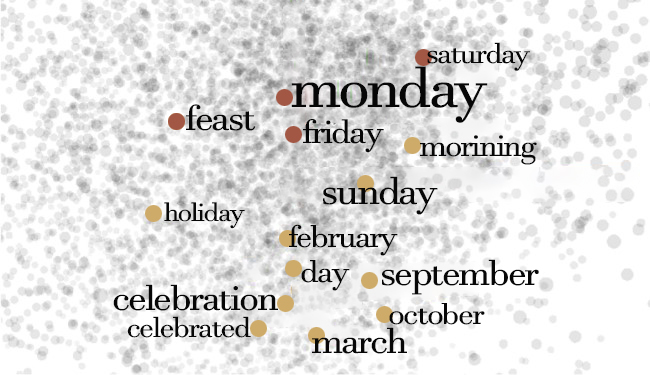
\includegraphics[width=6cm]{./Chapter5/Figures/word-graph.jpg}
\caption{分布式表示的可视化}
\label{fig:5-66}
\end{figure}
%-------------------------------------------

\parinterval  语言模型的词嵌入是通过词嵌入矩阵进行存储的,矩阵中的每一行对应了一个词的分布式表示结果。图\ref{fig:5-67}展示了一个词嵌入矩阵的实例。

%----------------------------------------------
\begin{figure}[htp]
\centering
%%%------------------------------------------------------------------------------------------------------------
\begin{tikzpicture}
\begin{scope}
\node [anchor=center,inner sep=2pt] (e) at (0,0) {\small{$e=w$}};
\node [anchor=west,inner sep=2pt] (c) at (e.east) {\small{$\textbf{C}$}};

\begin{pgfonlayer}{background}
\node [rectangle,inner sep=0.4em,draw,fill=blue!20!white] [fit = (e) (c)] (box) {};
\end{pgfonlayer}

\draw [->,thick] ([yshift=-1em]box.south)--([yshift=-0.1em]box.south) node [pos=0,below] (bottom1) {\small{单词$w$}};
\draw [->,thick] ([yshift=0.1em]box.north)--([yshift=1em]box.north) node [pos=1,above] (top1) {\scriptsize{$e$=(8,.2,-1,.9,...,1)}};
\node [anchor=north] (bottom2) at ([yshift=0.3em]bottom1.south) {\scriptsize{$w$=(0,0,1,0,...,0)}};
\node [anchor=south] (top2) at ([yshift=-0.3em]top1.north) {\small{$w$的分布式表示}};

{
\node [anchor=north west,fill=red!20!white] (cmatrix) at ([xshift=3em,yshift=1.0em]c.north east) {\scriptsize{$\begin{pmatrix} 1 & .2 & -.2 & 8 & ... & 0 \\ .6 & .8 & -2 & 1 & ... & -.2 \\ 8 & .2 & -1 & .9 & ... & 2.3 \\ 1 & 1.2 & -.9 & 3 & ... & .2 \\ ... & ... & ... & ... & ... & ... \\ 1 & .3 & 3 & .9 & ... & 5.1 \end{pmatrix}$}};
\node [anchor=west,inner sep=2pt,fill=red!30!white] (c) at (e.east) {\small{$\textbf{C}$}};
\draw [<-,thick] (c.east) -- ([xshift=3em]c.east);
}

{
\node [anchor=south,draw,fill=green!20!white] (e2) at ([yshift=1.5em]cmatrix.north) {\scriptsize{外部词嵌入系统得到的$\textbf{C}$}};
\draw [->,very thick,dashed] (e2.south) -- (cmatrix.north);
}

\end{scope}
\end{tikzpicture}
%%%------------------------------------------------------------------------------------------------------------


\caption{词嵌入矩阵$mathbf C$}
\label{fig:5-67}
\end{figure}
%-------------------------------------------

\parinterval  通常,有两种方法得到词嵌入矩阵。一种方法是把词嵌入作为语言模型的一部分进行训练,不过由于语言模型往往较复杂,这种方法非常耗时;另一种方法使用更加轻便的外部训练方法,如word2vec\cite{mikolov2013distributed}、Glove\cite{pennington2014glove}等。由于这些方法的效率较高,因此可以使用更大规模的数据得到更好的词嵌入结果。

%----------------------------------------------------------------------------------------
%    NEW SUB-SECTION
%----------------------------------------------------------------------------------------

\subsection{句子表示模型及预训练}

\parinterval  目前,词嵌入已经成为诸多自然语言处理系统的标配,也衍生出很多有趣的研究法方向,甚至有人开玩笑的喊出``embed everything''的口号。但是,冷静地看,词嵌入依旧存在一些问题:每个词都对应唯一的向量表示,那么对于一词多义现象,词义需要通过上下文进行区分,这时使用简单的词嵌入式是无法处理的。有一个著名的例子:

\begin{example}
Jobs was the CEO of {\red{\underline{apple}}}.

\qquad \qquad \; He finally ate the {\red{\underline{apple}}}.
\end{example}

\parinterval  这两句中``apple''的语义显然是不同的,第一句中的上下文``Jobs''和``CEO''可以帮助我们判断``apple''是一个公司名字,而不是水果。但是词嵌入只有一个结果,因此无法区分这两种情况。这个例子给我们一个启发:在一个句子中,不能孤立的看待单词,应同时考虑其上下文的信息。也就是需要一个能包含句子中上下文信息的表示模型。

%----------------------------------------------------------------------------------------
%    NEW SUBSUB-SECTION
%----------------------------------------------------------------------------------------

\subsubsection{简单的上下文表示模型}

\parinterval  回忆一下神经语言模型的结构,它需要在每个位置预测单词生成的概率。这个概率是由若干层神经网络进行计算后,通过输出层得到的。实际上,在送入输出层之前,系统已经得到了这个位置的一个向量(隐藏层的输出),因此可以把它看作是含有一部分上下文信息的表示结果。以RNN为例,图\ref{fig:5-68}展示了一个由四个词组成的句子,这里使用了一个两层循环神经网络对其进行建模。可以看到,对于第三个位置,RNN已经积累了从第1个单词到第3个单词的信息,因此可以看作是单词1-3(``乔布斯\ 就职\ 于'')的一种表示;另一方面,第4个单词的词嵌入可以看作是``苹果''自身的表示。这样,可以把第3 个位置RNN的输出和第4个位置的词嵌入进行合并,就得到了第4个位置上含有上下文信息的表示结果。从另一个角度说,这里得到了``苹果''的一种新的表示,它不仅包含苹果这个词自身的信息,也包含它前文的信息。

%----------------------------------------------
\begin{figure}[htp]
\centering
\begin{tikzpicture}
\begin{scope}
\tikzstyle{rnnnode} = [draw,inner sep=5pt,minimum width=4em,minimum height=1.5em,fill=green!30!white,blur shadow={shadow xshift=1pt,shadow yshift=-1pt}]
\node [anchor=west,rnnnode] (node11) at (0,0) {\scriptsize{RNN Cell}};
\node [anchor=west,rnnnode] (node12) at ([xshift=2em]node11.east) {\scriptsize{RNN Cell}};
\node [anchor=west,rnnnode] (node13) at ([xshift=2em]node12.east) {\scriptsize{RNN Cell}};
\node [anchor=west,rnnnode] (node14) at ([xshift=2em]node13.east) {\scriptsize{RNN Cell}};

\node [anchor=north,rnnnode,fill=red!30!white] (e1) at ([yshift=-1.2em]node11.south) {\scriptsize{embedding}};
\node [anchor=north,rnnnode,fill=red!30!white] (e2) at ([yshift=-1.2em]node12.south) {\scriptsize{embedding}};
\node [anchor=north,rnnnode,fill=red!30!white] (e3) at ([yshift=-1.2em]node13.south) {\scriptsize{embedding}};
\node [anchor=north,rnnnode,fill=red!30!white] (e4) at ([yshift=-1.2em]node14.south) {\scriptsize{embedding}};
\node [anchor=north] (w1) at ([yshift=-1em]e1.south) {\footnotesize{乔布斯}};
\node [anchor=north] (w2) at ([yshift=-1em]e2.south) {\footnotesize{任职}};
\node [anchor=north] (w3) at ([yshift=-1em]e3.south) {\footnotesize{于}};
\node [anchor=north] (w4) at ([yshift=-1em]e4.south) {\footnotesize{苹果}};

\draw [->,thick] ([yshift=0.1em]w1.north)--([yshift=-0.1em]e1.south);
\draw [->,thick] ([yshift=0.1em]w2.north)--([yshift=-0.1em]e2.south);
\draw [->,thick] ([yshift=0.1em]w3.north)--([yshift=-0.1em]e3.south);
\draw [->,thick] ([yshift=0.1em]w4.north)--([yshift=-0.1em]e4.south);

\draw [->,thick] ([yshift=0.1em]e1.north)--([yshift=-0.1em]node11.south);
\draw [->,thick] ([yshift=0.1em]e2.north)--([yshift=-0.1em]node12.south);
\draw [->,thick] ([yshift=0.1em]e3.north)--([yshift=-0.1em]node13.south);
\draw [->,thick] ([yshift=0.1em]e4.north)--([yshift=-0.1em]node14.south);

\node [anchor=south,rnnnode] (node21) at ([yshift=1.5em]node11.north) {\scriptsize{RNN Cell}};
\node [anchor=south,rnnnode] (node22) at ([yshift=1.5em]node12.north) {\scriptsize{RNN Cell}};
\node [anchor=south,rnnnode] (node23) at ([yshift=1.5em]node13.north) {\scriptsize{RNN Cell}};
\node [anchor=south,rnnnode] (node24) at ([yshift=1.5em]node14.north) {\scriptsize{RNN Cell}};

\node [anchor=south] (node31) at ([yshift=1.0em]node21.north) {\scriptsize{的表示}};
\node [anchor=south west] (node31new) at ([yshift=-0.3em]node31.north west) {\scriptsize{``乔布斯''}};
\node [anchor=south] (node32) at ([yshift=1.0em]node22.north) {\scriptsize{的表示\ \ \ }};
\node [anchor=south west] (node32new) at ([yshift=-0.3em]node32.north west) {\scriptsize{``乔布斯 任职''}};
\node [anchor=south] (node33) at ([yshift=1.0em]node23.north) {\scriptsize{的表示\ \ \ \ \ \ \ \ }};
\node [anchor=south west] (node33new) at ([yshift=-0.3em]node33.north west) {\scriptsize{``乔布斯 任职 于''}};
\node [anchor=south] (node34) at ([yshift=1.0em]node24.north) {\scriptsize{的表示\ \ \ \ \ \ \ \ }};
\node [anchor=south west] (node34new) at ([yshift=-0.3em]node34.north west) {\scriptsize{``乔布斯 任职 于 苹果''}};

\draw [->,thick] ([yshift=0.1em]node21.north)--([yshift=-0.1em]node31.south);
\draw [->,thick] ([yshift=0.1em]node22.north)--([yshift=-0.1em]node32.south);
\draw [->,thick] ([yshift=0.1em]node23.north)--([yshift=-0.1em]node33.south);
\draw [->,thick] ([yshift=0.1em]node24.north)--([yshift=-0.1em]node34.south);

\draw [->,thick] ([xshift=-1em]node21.west)--([xshift=-0.1em]node21.west);
\draw [->,thick] ([xshift=0.1em]node21.east)--([xshift=-0.1em]node22.west);
\draw [->,thick] ([xshift=0.1em]node22.east)--([xshift=-0.1em]node23.west);
\draw [->,thick] ([xshift=0.1em]node23.east)--([xshift=-0.1em]node24.west);
\draw [->,thick] ([xshift=0.1em]node24.east)--([xshift=1em]node24.east);

\draw [->,thick] ([yshift=0.1em]node11.north)--([yshift=-0.1em]node21.south);
\draw [->,thick] ([yshift=0.1em]node12.north)--([yshift=-0.1em]node22.south);
\draw [->,thick] ([yshift=0.1em]node13.north)--([yshift=-0.1em]node23.south);
\draw [->,thick] ([yshift=0.1em]node14.north)--([yshift=-0.1em]node24.south);

\draw [->,thick] ([xshift=-1em]node11.west)--([xshift=-0.1em]node11.west);
\draw [->,thick] ([xshift=0.1em]node11.east)--([xshift=-0.1em]node12.west);
\draw [->,thick] ([xshift=0.1em]node12.east)--([xshift=-0.1em]node13.west);
\draw [->,thick] ([xshift=0.1em]node13.east)--([xshift=-0.1em]node14.west);
\draw [->,thick] ([xshift=0.1em]node14.east)--([xshift=1em]node14.east);

{
\node [anchor=south] (toplabel1) at ([yshift=2em,xshift=-1.3em]node32new.north) {\footnotesize{``苹果''的表示:}};
\node [anchor=west,fill=blue!20!white,minimum width=3em] (toplabel2) at (toplabel1.east) {\footnotesize{上下文}};
}
{
\node [anchor=west,fill=red!20!white,minimum width=3em] (toplabel3) at (toplabel2.east) {\footnotesize{词}};
}

\begin{pgfonlayer}{background}
{
\node [rectangle,inner sep=2pt,draw,thick,dashed,red] [fit = (e4)] (r2) {};
\draw [->,thick,red] (r2.west) .. controls +(west:0.8) and +(south:2) .. ([xshift=1.3em]toplabel3.south);
}
{
\node [rectangle,inner sep=2pt,draw,thick,dashed,ublue,fill=white] [fit = (node33) (node33new)] (r1) {};
\draw [->,thick,ublue] ([xshift=-2em]r1.north) .. controls +(north:0.7) and +(south:0.7) .. ([xshift=-0.5em]toplabel2.south);
}
\end{pgfonlayer}

\end{scope}
\end{tikzpicture}
\caption{基于RNN的表示模型(词+上下文)}
\label{fig:5-68}
\end{figure}
%-------------------------------------------

\parinterval  在自然语言处理中,{\small\sffamily\bfseries{句子表示模型}}\index{句子表示模型}是指把输入的句子进行分布式表示。不过表示的形式不一定是一个单独的向量。现在广泛使用的句子表示模型可以被描述为:给定一个输入的句子$ \{ w_1,\dots ,w_m\} $,得到一个表示序列$ \{ \mathbf h_1,\dots ,\mathbf h_m\} $,其中$ h_i $是句子在第$ i $个位置的表示结果。$ \{ \mathbf h_1,\dots ,\mathbf h_m\} $就被看作是{\small\sffamily\bfseries{句子的表示}}\index{句子的表示},它可以被送入下游模块。比如,在机器翻译任务中,可以用这种模型表示源语言句子,然后通过这种表示结果进行目标语译文的生成;在序列标注(如词性标注)任务中,可以对输入的句子进行表示,然后在这个表示之上构建标签预测模块。很多自然语言处理任务都可以用句子表示模型进行建模,因此句子的表示模型也是应用最广泛的深度学习模型之一。而学习这种表示的过程也被称作{\small\sffamily\bfseries{表示学习}}\index{表示学习}(Representation Learning)\index{Representation Learning}。

\parinterval  句子表示模型有两种训练方法。最简单的方法是把它作为目标系统中的一个模块进行训练,比如把句子表示模型作为机器翻译系统的一部分。也就是,并不单独训练句子表示模型,而是把它作为一个内部模块放到其他系统中。另一种方法是把句子表示作为独立的模块,用外部系统进行训练,之后把训练好的表示模型放入目标系统中,再进行微调。这种方法构成了一种新的范式:预训练+微调(pre-training + fine-tuning)。图\ref{fig:5-69}对比了这两种不同的方法。

%----------------------------------------------
\begin{figure}[htp]
\centering
%%%------------------------------------------------------------------------------------------------------------
\begin{tikzpicture}

\begin{scope}

\node [anchor=west,draw,thick,minimum width=4em,minimum height=1.7em,fill=blue!20] (encoder) at (0,0) {模块};
\node [anchor=south,minimum width=4em,minimum height=1.7em] (space) at ([yshift=0.3em]encoder.north) {\footnotesize{目标系统}};

\begin{pgfonlayer}{background}
\node [rectangle,draw,thick,fill=red!20] [fit = (encoder) (space)] (system) {};
\end{pgfonlayer}

\node [anchor=north] (data) at ([yshift=-1em]system.south) {\scriptsize{\textbf{目标任务有标注数据}}};
\draw [->,thick] (data.north) -- ([yshift=-0.1em]system.south);
\node [anchor=north] (label) at ([yshift=-0em]data.south) {\scriptsize{(a) standard method}};

\end{scope}

\begin{scope}[xshift=2.8in]

\node [anchor=west,draw,dashed,thick,minimum width=4em,minimum height=1.7em,fill=blue!20] (encoder) at (0,0) {模块};
\node [anchor=south,minimum width=4em,minimum height=1.7em] (space) at ([yshift=0.3em]encoder.north) {\footnotesize{目标系统}};
\node [anchor=center,draw,thick,minimum width=4em,minimum height=1.7em,fill=green!20] (encoderpre) at ([xshift=-7em]encoder.center) {\footnotesize{语言模型}};
\draw [->,thick] (encoderpre.east) -- (encoder.west);

\begin{pgfonlayer}{background}
\node [rectangle,draw,thick,fill=red!20] [fit = (encoder) (space)] (system) {};
\end{pgfonlayer}

\node [anchor=north] (data) at ([yshift=-1em]system.south) {\scriptsize{\textbf{目标任务有标注数据}}};
\draw [->,thick] (data.north) -- ([yshift=-0.1em]system.south);
\node [anchor=north] (data2) at ([yshift=-1em,xshift=-7em]system.south) {\scriptsize{\textbf{大规模无标注数据}}};
\draw [->,thick] (data2.north) -- ([yshift=-0.1em]encoderpre.south);
\node [anchor=north] (label) at ([yshift=-0em,xshift=-4em]data.south) {\scriptsize{(b) pre-training + fine-tuning}};

\end{scope}

\end{tikzpicture}
%%%------------------------------------------------------------------------------------------------------------


\caption{表示模型的训练方法(与目标任务联合训练 vs 用外部任务预训练)}
\label{fig:5-69}
\end{figure}
%-------------------------------------------

\parinterval  目前,句子表示模型的预训练方法在多项自然语言处理任务上取得了很好的效果。预训练模型也成为了当今自然语言处理中的热点方向,相关系统也在很多评测任务上刷榜。除了上面提到的简单的神经语言模型的方法,还有各式各样基于预训练的表示模型被提出。接下来,会简单介绍其中比较有代表性的三种模型$\ \dash\ $ELMO、 GPT 和BERT。

%----------------------------------------------------------------------------------------
%    NEW SUBSUB-SECTION
%----------------------------------------------------------------------------------------

\subsubsection{ELMO模型}

\parinterval  ELMO(Embedding from Language Models)掀起了基于语言模型的预训练的热潮\cite{peters2018deep}。ELMO的论文也获得了自然语言处理领域顶级会议NAACL2018的最佳论文。

\parinterval  在ELMO中,作者认为词的表示应该能够包含丰富的句子结构信息,并且能够对多义词进行建模。而传统的词嵌入(例如word2vec)是上下文无关的,所以他们利用语言模型来获得一个上下文相关的预训练表示。EMLO基于双向LSTM语言模型\footnote{ LSTM(Long Short-Term Memory),即长短时记忆模型,是一种循环神经网络结构。},由一个正向语言模型和一个反向语言模型构成,目标函数是最大化这两个方向语言模型的似然(图\ref{fig:5-70})。简单来说,ELMO就是一个预训练好的双向语言模型,对于每个句子都可以生成相应的句子表示结果,这个结果会作为输入的特征被送入下游任务中。比如,ELMO在问答、文本蕴含、情感分析等多个任务中都表现出非常好的效果。

%----------------------------------------------
\begin{figure}[htp]
\centering
%%%------------------------------------------------------------------------------------------------------------
\begin{tikzpicture}
\begin{scope}[scale=1.2]

\node [anchor=west,draw,inner sep=4pt,fill=blue!20!white] (Lstm0) at (0,0) {\scriptsize{LSTM}};
\node [anchor=west,draw,inner sep=4pt,fill=blue!20!white] (Lstm1) at ([xshift=1em]Lstm0.east) {\scriptsize{LSTM}};
\node [anchor=west,inner sep=4pt] (sep) at ([xshift=0.5em]Lstm1.east) {\scriptsize{...}};
\node [anchor=west,draw,inner sep=4pt,fill=blue!20!white] (Lstm2) at ([xshift=0.5em]sep.east) {\scriptsize{LSTM}};

\node [anchor=south,draw,inner sep=4pt,fill=blue!20!white] (Lstm3) at ([yshift=1em]Lstm0.north) {\scriptsize{LSTM}};
\node [anchor=west,draw,inner sep=4pt,fill=blue!20!white] (Lstm4) at ([xshift=1em]Lstm3.east) {\scriptsize{LSTM}};
\node [anchor=west,inner sep=4pt] (sep1) at ([xshift=0.5em]Lstm4.east) {\scriptsize{...}};
\node [anchor=west,draw,inner sep=4pt,fill=blue!20!white] (Lstm5) at ([xshift=0.5em]sep1.east) {\scriptsize{LSTM}};

\node [rectangle,rounded corners,draw=black!50,densely dashed,inner sep=0.4em] [fit = (Lstm0) (Lstm2) (Lstm3) (Lstm5)] (inputshadow) {};

\node [anchor=north,draw,inner sep=4pt,fill=ugreen!20!white,minimum width=2em] (e1) at ([xshift=-2em,yshift=-1em]Lstm2.south) {\scriptsize{$\textbf{e}_1$}};
\node [anchor=west,draw,inner sep=4pt,fill=ugreen!20!white,minimum width=2em] (e2) at ([xshift=1em]e1.east) {\scriptsize{$\textbf{e}_2$}};
\node [anchor=west,inner sep=4pt] (sep5) at ([xshift=1em]e2.east) {\scriptsize{...}};
\node [anchor=west,draw,inner sep=4pt,fill=ugreen!20!white,minimum width=2em] (e3) at ([xshift=1em]sep5.east) {\scriptsize{$\textbf{e}_m$}};
\node [anchor=south] (word1) at ([yshift=-1.5em]e1.south) {\footnotesize {Once}};
\node [anchor=south] (word2) at ([yshift=-1.6em]e2.south) {\footnotesize {upon}};
\node [anchor=south] (wordseq) at ([yshift=-1.5em]sep5.south) {\footnotesize{...}};
\node [anchor=south] (word3) at ([yshift=-1.5em]e3.south) {\footnotesize {island}};

\node [anchor=south,draw,inner sep=4pt,fill=yellow!30,minimum width=2em] (t1) at ([xshift=-2em,yshift=1em]Lstm5.north) {\scriptsize{$\textbf{h}_1$}};
\node [anchor=west,draw,inner sep=4pt,fill=yellow!30,minimum width=2em] (t2) at ([xshift=1em]t1.east) {\scriptsize{$\textbf{h}_2$}};
\node [anchor=west,inner sep=4pt] (sep6) at ([xshift=1em]t2.east) {\scriptsize{...}};
\node [anchor=west,draw,inner sep=4pt,fill=yellow!30,minimum width=2em] (t3) at ([xshift=1em]sep6.east) {\scriptsize{$\textbf{h}_m$}};

\node [anchor=west,draw,inner sep=4pt,fill=blue!20!white] (Lstm6) at ([xshift=1.5em]Lstm2.east) {\scriptsize{LSTM}};
\node [anchor=west,draw,inner sep=4pt,fill=blue!20!white] (Lstm7) at ([xshift=1em]Lstm6.east) {\scriptsize{LSTM}};
\node [anchor=west,inner sep=4pt] (sep3) at ([xshift=0.5em]Lstm7.east) {\scriptsize{...}};
\node [anchor=west,draw,inner sep=4pt,fill=blue!20!white] (Lstm8) at ([xshift=0.5em]sep3.east) {\scriptsize{LSTM}};

\node [anchor=south,draw,inner sep=4pt,fill=blue!20!white] (Lstm9) at ([yshift=1em]Lstm6.north) {\scriptsize{LSTM}};
\node [anchor=west,draw,inner sep=4pt,fill=blue!20!white] (Lstm10) at ([xshift=1em]Lstm9.east) {\scriptsize{LSTM}};
\node [anchor=west,inner sep=4pt] (sep4) at ([xshift=0.5em]Lstm10.east) {\scriptsize{...}};
\node [anchor=west,draw,inner sep=4pt,fill=blue!20!white] (Lstm11) at ([xshift=0.5em]sep4.east) {\scriptsize{LSTM}};

\node [rectangle,rounded corners,draw=black!50,densely dashed,inner sep=0.4em] [fit = (Lstm6) (Lstm8) (Lstm9) (Lstm11)] (inputshadow) {};

\draw [->] ([xshift=0.1em]Lstm0.east) -- ([xshift=-0.1em]Lstm1.west);
\draw [->] ([xshift=0.1em]Lstm1.east) -- ([xshift=0.1em]sep.west);
\draw [->] ([xshift=-0.1em]sep.east) -- ([xshift=-0.1em]Lstm2.west);

\draw [->] ([xshift=0.1em]Lstm3.east) -- ([xshift=-0.1em]Lstm4.west);
\draw [->] ([xshift=0.1em]Lstm4.east) -- ([xshift=0.1em]sep1.west);
\draw [->] ([xshift=-0.1em]sep1.east) -- ([xshift=-0.1em]Lstm5.west);

\draw [->] ([yshift=0.1em]Lstm0.north) -- ([yshift=-0.1em]Lstm3.south);
\draw [->] ([yshift=0.1em]Lstm1.north) -- ([yshift=-0.1em]Lstm4.south);
\draw [->] ([yshift=0.1em]Lstm2.north) -- ([yshift=-0.1em]Lstm5.south);

\draw [->] ([xshift=-0.1em]Lstm7.west) -- ([xshift=0.1em]Lstm6.east);
\draw [->] ([xshift=0.1em]sep3.west) -- ([xshift=0.1em]Lstm7.east);
\draw [->] ([xshift=-0.1em]Lstm8.west) -- ([xshift=-0.1em]sep3.east);

\draw [->] ([xshift=-0.1em]Lstm10.west) -- ([xshift=0.1em]Lstm9.east);
\draw [->] ([xshift=0.1em]sep4.west) -- ([xshift=0.1em]Lstm10.east);
\draw [->] ([xshift=-0.1em]Lstm11.west) -- ([xshift=-0.1em]sep4.east);

\draw [->] ([yshift=0.1em]Lstm6.north) -- ([yshift=-0.1em]Lstm9.south);
\draw [->] ([yshift=0.1em]Lstm7.north) -- ([yshift=-0.1em]Lstm10.south);
\draw [->] ([yshift=0.1em]Lstm8.north) -- ([yshift=-0.1em]Lstm11.south);

\draw [->] ([yshift=0.1em]e1.north) -- ([yshift=-0.12em]Lstm0.south);
\draw [->] ([yshift=0.1em]e1.north) -- ([yshift=-0.12em]Lstm6.south);
\draw [->] ([yshift=0.1em]e2.north) -- ([yshift=-0.12em]Lstm1.south);
\draw [->] ([yshift=0.1em]e2.north) -- ([yshift=-0.12em]Lstm7.south);
\draw [->] ([yshift=0.1em]e3.north) -- ([yshift=-0.12em]Lstm2.south);
\draw [->] ([yshift=0.1em]e3.north) -- ([yshift=-0.12em]Lstm8.south);

\draw [->] ([yshift=0.1em]Lstm3.north) -- ([xshift=-0.05em,yshift=-0.12em]t1.south);
\draw [->] ([yshift=0.1em]Lstm9.north) -- ([yshift=-0.12em]t1.south);
\draw [->] ([yshift=0.1em]Lstm4.north) -- ([xshift=-0.05em,yshift=-0.12em]t2.south);
\draw [->] ([yshift=0.1em]Lstm10.north) -- ([yshift=-0.12em]t2.south);
\draw [->] ([yshift=0.1em]Lstm5.north) -- ([xshift=-0.05em,yshift=-0.12em]t3.south);
\draw [->] ([yshift=0.1em]Lstm11.north) -- ([yshift=-0.12em]t3.south);

\end{scope}
\end{tikzpicture}
%%%------------------------------------------------------------------------------------------------------------


\caption{ELMO模型结构}
\label{fig:5-70}
\end{figure}
%-------------------------------------------

%----------------------------------------------------------------------------------------
%    NEW SUBSUB-SECTION
%----------------------------------------------------------------------------------------

\subsubsection{GPT模型}

\parinterval  GPT(Generative Pre-Training)也是一种基于语言建模的句子表示模型\cite{radford2018improving}。该工作的贡献在于利用Transformer结构代替了LSTM。而且该模型基于Pre-training + Fine-tuning的框架,预训练的结果将作为下游系统的句子表示模块的参数初始值,因此可以更好的适应目标任务。

\parinterval  GPT模型仍然使用标准的语言建模的思路,即通过前$ n-1 $个词预测第$ n $个词。但是在网络结构上,GPT模型使用了Transformer(图\ref{fig:5-71}),而且模型参数会在目标任务上进行有监督的微调。与ELMO模型的做法不同,GPT不需要对目标任务构建新的模型结构,而是直接在Transformer语言表示模型的最后一层加上Softmax层作为任务的输出层。实验结果证明,GPT模型的性能较ELMO模型更为优越,在12个NLP任务中取得了9个任务当时最好的结果。

%----------------------------------------------
\begin{figure}[htp]
\centering
%%%------------------------------------------------------------------------------------------------------------
\begin{tikzpicture}
\begin{scope}[scale=1.2]

\node [anchor=west,draw,inner sep=4pt,fill=blue!20!white,minimum width=3em] (Trm0) at (0,0) {\scriptsize{TRM}};
\node [anchor=west,draw,inner sep=4pt,fill=blue!20!white,minimum width=3em] (Trm1) at ([xshift=1em]Trm0.east) {\scriptsize{TRM}};
\node [anchor=west,draw,inner sep=4pt,fill=blue!20!white,minimum width=3em] (Trm2) at ([xshift=1em]Trm1.east) {\scriptsize{TRM}};
\node [anchor=west,draw,inner sep=4pt,fill=blue!20!white,minimum width=3em] (Trm3) at ([xshift=1em]Trm2.east) {\scriptsize{TRM}};
\node [anchor=west,inner sep=4pt] (sep) at ([xshift=1em]Trm3.east) {\scriptsize{...}};
\node [anchor=west,draw,inner sep=4pt,fill=blue!20!white,minimum width=3em] (Trm4) at ([xshift=1em]sep.east) {\scriptsize{TRM}};

\node [anchor=south,draw,inner sep=4pt,fill=blue!20!white,minimum width=3em] (Trm5) at ([yshift=1.2em]Trm0.north) {\scriptsize{TRM}};
\node [anchor=west,draw,inner sep=4pt,fill=blue!20!white,minimum width=3em] (Trm6) at ([xshift=1em]Trm5.east) {\scriptsize{TRM}};
\node [anchor=west,draw,inner sep=4pt,fill=blue!20!white,minimum width=3em] (Trm7) at ([xshift=1em]Trm6.east) {\scriptsize{TRM}};
\node [anchor=west,draw,inner sep=4pt,fill=blue!20!white,minimum width=3em] (Trm8) at ([xshift=1em]Trm7.east) {\scriptsize{TRM}};
\node [anchor=west,inner sep=4pt] (sep1) at ([xshift=1em]Trm8.east) {\scriptsize{...}};
\node [anchor=west,draw,inner sep=4pt,fill=blue!20!white,minimum width=3em] (Trm9) at ([xshift=1em]sep1.east) {\scriptsize{TRM}};

\node [rectangle,rounded corners,draw=black!50,densely dashed,inner sep=0.4em] [fit = (Trm0) (Trm4) (Trm5) (Trm9)] (inputshadow) {};

\node [anchor=north,draw,inner sep=4pt,fill=ugreen!20!white,minimum width=2em] (e1) at ([yshift=-1.2em]Trm0.south) {\scriptsize{$\textbf{e}_1$}};
\node [anchor=north,draw,inner sep=4pt,fill=ugreen!20!white,minimum width=2em] (e2) at ([yshift=-1.2em]Trm1.south) {\scriptsize{$\textbf{e}_2$}};
\node [anchor=north,draw,inner sep=4pt,fill=ugreen!20!white,minimum width=2em] (e3) at ([yshift=-1.2em]Trm2.south) {\scriptsize{$\textbf{e}_3$}};
\node [anchor=north,draw,inner sep=4pt,fill=ugreen!20!white,minimum width=2em] (e4) at ([yshift=-1.2em]Trm3.south) {\scriptsize{$\textbf{e}_4$}};
\node [anchor=north,inner sep=4pt] (sep5) at ([yshift=-1em]sep.south) {\scriptsize{...}};
\node [anchor=north,draw,inner sep=4pt,fill=ugreen!20!white,minimum width=2em] (e5) at ([yshift=-1.2em]Trm4.south) {\scriptsize{$\textbf{e}_m$}};
\node [anchor=south] (word1) at ([yshift=-1.5em]e1.south) {\footnotesize {Once}};
\node [anchor=south] (word2) at ([yshift=-1.6em]e2.south) {\footnotesize {upon}};
\node [anchor=south] (word3) at ([yshift=-1.5em]e3.south) {\footnotesize {a}};
\node [anchor=south] (word4) at ([yshift=-1.5em]e4.south) {\footnotesize {time}};
\node [anchor=south] (wordseq) at ([yshift=-2.0em]sep5.south) {\footnotesize{...}};
\node [anchor=south] (word4) at ([yshift=-1.5em]e5.south) {\footnotesize {island}};

\node [anchor=south,draw,inner sep=4pt,fill=yellow!30,minimum width=2em] (t1) at ([yshift=1.2em]Trm5.north) {\scriptsize{$\textbf{h}_1$}};
\node [anchor=south,draw,inner sep=4pt,fill=yellow!30,minimum width=2em] (t2) at ([yshift=1.2em]Trm6.north) {\scriptsize{$\textbf{h}_2$}};
\node [anchor=south,draw,inner sep=4pt,fill=yellow!30,minimum width=2em] (t3) at ([yshift=1.2em]Trm7.north) {\scriptsize{$\textbf{h}_3$}};
\node [anchor=south,draw,inner sep=4pt,fill=yellow!30,minimum width=2em] (t4) at ([yshift=1.2em]Trm8.north) {\scriptsize{$\textbf{h}_4$}};
\node [anchor=south,inner sep=4pt] (sep6) at ([yshift=1em]sep1.north) {\scriptsize{...}};
\node [anchor=south,draw,inner sep=4pt,fill=yellow!30,minimum width=2em] (t5) at ([yshift=1.2em]Trm9.north) {\scriptsize{$\textbf{h}_m$}};

\node [anchor=west,draw,inner sep=3pt,fill=blue!20!white,minimum width=1em] (Lt1) at ([yshift=1.2em]t1.west) {\tiny{TRM}};
\node [anchor=west] (Lt2) at ([xshift=-0.1em]Lt1.east) {\tiny{: Transformer}};

\draw [->] ([yshift=0.1em]e1.north) -- ([yshift=-0.1em]Trm0.south);
\draw [->] ([yshift=0.1em]e1.north) -- ([yshift=-0.1em]Trm1.260);
\draw [->] ([yshift=0.1em]e1.north) -- ([yshift=-0.1em]Trm2.260);
\draw [->] ([yshift=0.1em]e1.north) -- ([yshift=-0.1em]Trm3.260);
\draw [->] ([yshift=0.1em]e1.north) -- ([yshift=-0.1em]Trm4.260);
\draw [->] ([yshift=0.1em]e2.north) -- ([yshift=-0.1em]Trm1.south);

\draw [->] ([yshift=0.1em]e3.north) -- ([yshift=-0.1em]Trm2.south);
\draw [->] ([yshift=0.1em]e3.north) -- ([yshift=-0.1em]Trm3.260);
\draw [->] ([yshift=0.1em]e3.north) -- ([yshift=-0.1em]Trm4.260);
\draw [->] ([yshift=0.1em]e4.north) -- ([yshift=-0.1em]Trm3.south);
\draw [->] ([yshift=0.1em]e5.north) -- ([yshift=-0.1em]Trm4.south);

\draw [->] ([yshift=0.1em]Trm0.north) -- ([yshift=-0.1em]Trm5.south);
\draw [->] ([yshift=0.1em]Trm0.north) -- ([yshift=-0.1em]Trm6.260);
\draw [->] ([yshift=0.1em]Trm0.north) -- ([yshift=-0.1em]Trm7.260);
\draw [->] ([yshift=0.1em]Trm0.north) -- ([yshift=-0.1em]Trm8.260);
\draw [->] ([yshift=0.1em]Trm0.north) -- ([yshift=-0.1em]Trm9.260);
\draw [->] ([yshift=0.1em]Trm1.north) -- ([yshift=-0.1em]Trm6.south);
\draw [->] ([yshift=0.1em]Trm2.north) -- ([yshift=-0.1em]Trm7.south);
\draw [->] ([yshift=0.1em]Trm2.north) -- ([yshift=-0.1em]Trm8.260);
\draw [->] ([yshift=0.1em]Trm2.north) -- ([yshift=-0.1em]Trm9.260);
\draw [->] ([yshift=0.1em]Trm3.north) -- ([yshift=-0.1em]Trm8.south);
\draw [->] ([yshift=0.1em]Trm4.north) -- ([yshift=-0.1em]Trm9.south);

\draw [->] ([yshift=0.1em]Trm5.north) -- ([yshift=-0.1em]t1.south);
\draw [->] ([yshift=0.1em]Trm6.north) -- ([yshift=-0.1em]t2.south);
\draw [->] ([yshift=0.1em]Trm7.north) -- ([yshift=-0.1em]t3.south);
\draw [->] ([yshift=0.1em]Trm8.north) -- ([yshift=-0.1em]t4.south);
\draw [->] ([yshift=0.1em]Trm9.north) -- ([yshift=-0.1em]t5.south);

\end{scope}
\end{tikzpicture}
%%%------------------------------------------------------------------------------------------------------------


\caption{GPT模型结构}
\label{fig:5-71}
\end{figure}
%-------------------------------------------
\vspace{-0.5em}
%----------------------------------------------------------------------------------------
%    NEW SUBSUB-SECTION
%----------------------------------------------------------------------------------------

\subsubsection{BERT模型}

\parinterval  BERT(Bidirectional Encoder Representations from Transformers)是另一个非常有代表性的基于预训练的句子表示模型\cite{DBLP:conf/naacl/DevlinCLT19}。某种意义上,BERT把基于预训练的句子表示模型推向了新的高潮。BERT的论文也获得了NAACL2019最佳论文奖。

\parinterval  与传统语言模型的训练目标不同,BERT不使用预测下一个词作为训练目标,而是提出了两个新的任务。

\begin{itemize}
\vspace{0.5em}
\item 第一个任务被称为Masked LM。在输入的词序列中随机地挡住一定量的的词(比如15\%的单词被挡住),然后让模型去预测挡住的这些词。这个过程有些类似于英语考试中的完形填空。这么做的好处是,模型能够从多个方向去预测这些被遮罩住的词(图\ref{fig:5-72}),而不是像传统语言模型一样从单个方向预测(自左向右或者自右向左)。Masked LM的思想也影响了很多预训练模型的设计。
\vspace{0.5em}
\item 第二个任务是预测下一个句子。当选择句子a与b作为预训练样本时,b有一半几率可能是a的下一句,也有一半几率来自语料库的随机句子,从而可以更好地学习句子之间的相关性。
\vspace{0.5em}
\end{itemize}

\parinterval  BERT的训练目标就是最小化这两个任务上的损失函数。实验结果证明,BERT\\模型的性能十分强劲,在11个NLP任务上取得了当时最好的性能。

%----------------------------------------------
\begin{figure}[htp]
\centering
%%%------------------------------------------------------------------------------------------------------------
\begin{tikzpicture}
\begin{scope}[scale=1.2]

\node [anchor=west,draw,inner sep=4pt,fill=blue!20!white,minimum width=3em] (Trm0) at (0,0) {\scriptsize{TRM}};
\node [anchor=west,draw,inner sep=4pt,fill=blue!20!white,minimum width=3em] (Trm1) at ([xshift=1em]Trm0.east) {\scriptsize{TRM}};
\node [anchor=west,draw,inner sep=4pt,fill=blue!20!white,minimum width=3em] (Trm2) at ([xshift=1em]Trm1.east) {\scriptsize{TRM}};
\node [anchor=west,draw,inner sep=4pt,fill=blue!20!white,minimum width=3em] (Trm3) at ([xshift=1em]Trm2.east) {\scriptsize{TRM}};
\node [anchor=west,inner sep=4pt] (sep) at ([xshift=1em]Trm3.east) {\scriptsize{...}};
\node [anchor=west,draw,inner sep=4pt,fill=blue!20!white,minimum width=3em] (Trm4) at ([xshift=1em]sep.east) {\scriptsize{TRM}};

\node [anchor=south,draw,inner sep=4pt,fill=blue!20!white,minimum width=3em] (Trm5) at ([yshift=1.2em]Trm0.north) {\scriptsize{TRM}};
\node [anchor=west,draw,inner sep=4pt,fill=blue!20!white,minimum width=3em] (Trm6) at ([xshift=1em]Trm5.east) {\scriptsize{TRM}};
\node [anchor=west,draw,inner sep=4pt,fill=blue!20!white,minimum width=3em] (Trm7) at ([xshift=1em]Trm6.east) {\scriptsize{TRM}};
\node [anchor=west,draw,inner sep=4pt,fill=blue!20!white,minimum width=3em] (Trm8) at ([xshift=1em]Trm7.east) {\scriptsize{TRM}};
\node [anchor=west,inner sep=4pt] (sep1) at ([xshift=1em]Trm8.east) {\scriptsize{...}};
\node [anchor=west,draw,inner sep=4pt,fill=blue!20!white,minimum width=3em] (Trm9) at ([xshift=1em]sep1.east) {\scriptsize{TRM}};

\node [rectangle,rounded corners,draw=black!50,densely dashed,inner sep=0.4em] [fit = (Trm0) (Trm4) (Trm5) (Trm9)] (inputshadow) {};

\node [anchor=north,draw,inner sep=4pt,fill=ugreen!20!white,minimum width=2em] (e1) at ([yshift=-1.2em]Trm0.south) {\scriptsize{$\textbf{e}_1$}};
\node [anchor=north,draw,inner sep=4pt,fill=ugreen!20!white,minimum width=2em] (e2) at ([yshift=-1.2em]Trm1.south) {\scriptsize{$\textbf{e}_2$}};
\node [anchor=north,draw,inner sep=4pt,fill=ugreen!20!white,minimum width=2em] (e3) at ([yshift=-1.2em]Trm2.south) {\scriptsize{$\textbf{e}_3$}};
\node [anchor=north,draw,inner sep=4pt,fill=ugreen!20!white,minimum width=2em] (e4) at ([yshift=-1.2em]Trm3.south) {\scriptsize{$\textbf{e}_4$}};
\node [anchor=north,inner sep=4pt] (sep5) at ([yshift=-1em]sep.south) {\scriptsize{...}};
\node [anchor=north,draw,inner sep=4pt,fill=ugreen!20!white,minimum width=2em] (e5) at ([yshift=-1.2em]Trm4.south) {\scriptsize{$\textbf{e}_m$}};
\node [anchor=south] (word1) at ([yshift=-1.5em]e1.south) {\footnotesize {Once}};
\node [anchor=south] (word2) at ([yshift=-1.7em]e2.south) {\footnotesize {[MASK]}};
\node [anchor=south] (word3) at ([yshift=-1.5em]e3.south) {\footnotesize {a}};
\node [anchor=south] (word4) at ([yshift=-1.5em]e4.south) {\footnotesize {time}};
\node [anchor=south] (wordseq) at ([yshift=-2.0em]sep5.south) {\footnotesize{...}};
\node [anchor=south] (word4) at ([yshift=-1.5em]e5.south) {\footnotesize {island}};

\node [anchor=south,draw,inner sep=4pt,fill=yellow!30,minimum width=2em] (t1) at ([yshift=1.2em]Trm5.north) {\scriptsize{$\textbf{h}_1$}};
\node [anchor=south,draw,inner sep=4pt,fill=yellow!30,minimum width=2em] (t2) at ([yshift=1.2em]Trm6.north) {\scriptsize{$\textbf{h}_2$}};
\node [anchor=south,draw,inner sep=4pt,fill=yellow!30,minimum width=2em] (t3) at ([yshift=1.2em]Trm7.north) {\scriptsize{$\textbf{h}_3$}};
\node [anchor=south,draw,inner sep=4pt,fill=yellow!30,minimum width=2em] (t4) at ([yshift=1.2em]Trm8.north) {\scriptsize{$\textbf{h}_4$}};
\node [anchor=south,inner sep=4pt] (sep6) at ([yshift=1em]sep1.north) {\scriptsize{...}};
\node [anchor=south,draw,inner sep=4pt,fill=yellow!30,minimum width=2em] (t5) at ([yshift=1.2em]Trm9.north) {\scriptsize{$\textbf{h}_m$}};

\node [anchor=west,draw,inner sep=3pt,fill=blue!20!white,minimum width=1em] (Lt1) at ([yshift=1.2em]t1.west) {\tiny{TRM}};
\node [anchor=west] (Lt2) at ([xshift=-0.1em]Lt1.east) {\tiny{: Transformer}};

\draw [->] ([yshift=0.1em]e1.north) -- ([yshift=-0.1em]Trm0.south);
\draw [->] ([yshift=0.1em]e1.north) -- ([yshift=-0.1em]Trm1.south);
\draw [->] ([yshift=0.1em]e1.north) -- ([yshift=-0.1em]Trm2.south);
\draw [->] ([yshift=0.1em]e1.north) -- ([yshift=-0.1em]Trm3.south);
\draw [->] ([yshift=0.1em]e1.north) -- ([yshift=-0.1em]Trm4.south);
\draw [->] ([yshift=0.1em]e2.north) -- ([yshift=-0.1em]Trm1.south);
\draw [->] ([yshift=0.1em]e3.north) -- ([yshift=-0.1em]Trm0.south);
\draw [->] ([yshift=0.1em]e3.north) -- ([yshift=-0.1em]Trm1.south);
\draw [->] ([yshift=0.1em]e3.north) -- ([yshift=-0.1em]Trm2.south);
\draw [->] ([yshift=0.1em]e3.north) -- ([yshift=-0.1em]Trm3.south);
\draw [->] ([yshift=0.1em]e3.north) -- ([yshift=-0.1em]Trm4.south);
\draw [->] ([yshift=0.1em]e4.north) -- ([yshift=-0.1em]Trm3.south);
\draw [->] ([yshift=0.1em]e5.north) -- ([yshift=-0.1em]Trm4.south);

\draw [->] ([yshift=0.1em]Trm0.north) -- ([yshift=-0.1em]Trm5.south);
\draw [->] ([yshift=0.1em]Trm0.north) -- ([yshift=-0.1em]Trm6.south);
\draw [->] ([yshift=0.1em]Trm0.north) -- ([yshift=-0.1em]Trm8.south);
\draw [->] ([yshift=0.1em]Trm0.north) -- ([yshift=-0.1em]Trm9.south);
\draw [->] ([yshift=0.1em]Trm1.north) -- ([yshift=-0.1em]Trm6.south);
\draw [->] ([yshift=0.1em]Trm2.north) -- ([yshift=-0.1em]Trm5.south);
\draw [->] ([yshift=0.1em]Trm2.north) -- ([yshift=-0.1em]Trm6.south);
\draw [->] ([yshift=0.1em]Trm2.north) -- ([yshift=-0.1em]Trm7.south);
\draw [->] ([yshift=0.1em]Trm2.north) -- ([yshift=-0.1em]Trm8.south);
\draw [->] ([yshift=0.1em]Trm2.north) -- ([yshift=-0.1em]Trm9.south);
\draw [->] ([yshift=0.1em]Trm3.north) -- ([yshift=-0.1em]Trm8.south);
\draw [->] ([yshift=0.1em]Trm4.north) -- ([yshift=-0.1em]Trm9.south);

\draw [->] ([yshift=0.1em]Trm5.north) -- ([yshift=-0.1em]t1.south);
\draw [->] ([yshift=0.1em]Trm6.north) -- ([yshift=-0.1em]t2.south);
\draw [->] ([yshift=0.1em]Trm7.north) -- ([yshift=-0.1em]t3.south);
\draw [->] ([yshift=0.1em]Trm8.north) -- ([yshift=-0.1em]t4.south);
\draw [->] ([yshift=0.1em]Trm9.north) -- ([yshift=-0.1em]t5.south);

\end{scope}
\end{tikzpicture}
%%%------------------------------------------------------------------------------------------------------------


\caption{BERT模型结构}
\label{fig:5-72}
\end{figure}
%-------------------------------------------
\vspace{-0.5em}

%----------------------------------------------------------------------------------------
%    NEW SUUBSUB-SECTION
%----------------------------------------------------------------------------------------

\subsubsection{为什么要预训练?}

\parinterval  基于预训练的句子表示模型确实给自然语言处理带来了新的思路。相比传统的基于目标任务的建模和训练方法,预训练有如下优势:

\begin{itemize}
\vspace{0.5em}
\item 目标任务依赖有指导训练,但是带标注的数据往往十分有限。预训练模型并不依赖带标注数据,因此可以从更大规模的无标注数据(比如训练语言模型中使用的纯文本数据)学习知识,这使得预训练模型可以捕捉更加通用的语言规律,甚至有时候会具有一些``常识''\footnote{关于自然语言处理系统是否具有常识也存在不同的观点。从一些任务上的实验结果上看,很多模型确实能够进行一些常识性推理。但是,当问题的难度增加时,绝大多数模型还无法做到人类的水平。};
\vspace{0.5em}
\item 由于预训练并不依赖具体的目标任务,因此不会对目标任务产生过拟合,模型具有较好的泛化能力;
\vspace{0.5em}
\item 从优化的角度,预训练相当于将模型``初始化''到参数空间中优质解密度更高的区域(图\ref{fig:5-73}),下游任务更容易通过微调找到更好的参数(面向具体任务)。此外,也有实验表明预训练可以让模型参数落到损失函数曲面比较光滑的区域,这样能够避免下游任务在凸凹不平的损失函数曲面上陷入局部最优。
\vspace{0.5em}
\end{itemize}

%----------------------------------------------
\begin{figure}[htp]
\centering
%%%------------------------------------------------------------------------------------------------------------
\begin{tikzpicture}
\draw[name path=ellipse,thick] (0,0) circle[x radius = 2, y radius = 1];
\node[rectangle,minimum size=0.1em,inner sep=2pt,fill=red] (p1) at (0.2,0.5) {};
\node[rectangle,minimum size=0.1em,inner sep=2pt,fill=red] (p2) at (0.3,0.6) {};
\node[rectangle,minimum size=0.1em,inner sep=2pt,fill=red] (p3) at (0.1,-0.1) {};
\node[rectangle,minimum size=0.1em,inner sep=2pt,fill=red] (p4) at (0.4,0) {};
\node[rectangle,minimum size=0.1em,inner sep=2pt,fill=red] (p5) at (0.5,0.3) {};
\node[rectangle,minimum size=0.1em,inner sep=2pt,fill=red] (p6) at (0.6,0.1) {};
\node[rectangle,minimum size=0.1em,inner sep=2pt,fill=red] (p7) at (0.7,-0.1) {};
\node[rectangle,minimum size=0.1em,inner sep=2pt,fill=red] (p8) at (-1.2,0.4) {};
\node[rectangle,minimum size=0.1em,inner sep=2pt,fill=red] (p9) at (-1.0,-0.3) {};
\node[rectangle,minimum size=0.1em,inner sep=2pt,fill=red] (p10) at (-0.1,-0.8) {};

\begin{pgfonlayer}{background}
{
\node [rectangle,inner sep=0.4em,draw,blue] [fit = (p1) (p2) (p3) (p4) (p5) (p6)] (area) {};
}
\end{pgfonlayer}

\draw [->] (2.5,-0.7) -- (1.8,-0.5) node [pos=0,right] {\scriptsize{模型参数解空间}};

{
\draw [->] (2.0,0.7) -- (area.20) node [pos=0,right] {\scriptsize{优质解高密度区域(预训练)}};
}
{
\draw [->] (-2.0,0.7) -- (p8.west) node [pos=0,left] {\scriptsize{游离的解}};
}

\end{tikzpicture}
%%%------------------------------------------------------------------------------------------------------------


\caption{模型的参数空间}
\label{fig:5-73}
\end{figure}
%-------------------------------------------

%----------------------------------------------------------------------------------------
%    NEW SECTION
%----------------------------------------------------------------------------------------

\sectionnewpage
\section{小结及深入阅读}

\parinterval  神经网络为解决自然语言处理问题提供了全新的思路。而所谓深度学习也是建立在多层神经网络结构之上的一系列模型和方法。本章从神经网络的基本概念到其在语言建模中的应用进行了概述。由于篇幅所限,这里无法覆盖所有神经网络和深度学习的相关内容,感兴趣的读者可以进一步阅读《Neural Network Methods in Natural Language Processing》\cite{goldberg2017neural}和《Deep Learning》\cite{Goodfellow-et-al-2016}。此外,也有很多研究方向值得关注:

\begin{itemize}
\vspace{0.5em}
\item 端到端学习是神经网络方法的特点之一。这样,系统开发者不需要设计输入和输出的隐含结构,甚至连特征工程都不再需要。但是,另一方面,由于这种端到端学习完全由神经网络自行完成,整个学习过程没有人的先验知识做指导,导致学习的结构和参数很难进行解释。针对这个问题也有很多研究者进行{\small\sffamily\bfseries{可解释机器学习}}\index{可解释机器学习}(Explainable Machine Learning)\index{Explainable Machine Learning}的研究\cite{guidotti2018survey}\cite{koh2017understanding}。对于自然语言处理,方法的可解释性是十分必要的。从另一个角度说,如何使用先验知识改善端到端学习也是很多人关注的方向\cite{arthur2016incorporating}\cite{Zhang2017PriorKI},比如,如何使用句法知识改善自然语言处理模型\cite{zollmann2006syntax}\cite{charniak2003syntax}\cite{stahlberg2016syntactically}。
\vspace{0.5em}
\item 词嵌入是自然语言处理近些年的重要进展。所谓“嵌入”是一类方法,理论上,把一个事物进行分布式表示的过程都可以被看作是广义上的“嵌入”。基于这种思想的表示学习也成为了自然语言处理中的前沿方法。比如,如何对树结构,甚至图结构进行分布式表示\cite{plank2013embedding}\cite{perozzi2014deepwalk}成为了分析自然语言的重要方法。此外,除了语言建模,还有很多方式可以进行词嵌入的学习,比如,SENNA\cite{collobert2011natural}、word2vec\cite{mikolov2013efficient}\cite{mikolov2013distributed}、Glove\cite{pennington2014glove}、CoVe\cite{mccann2017learned}等。
\vspace{0.5em}
\item 预训练是表示学习的重要产物。预训练已经在图像处理等领域得到应用。在自然语言处理中,以BERT为代表的预训练模型席卷了很多自然语言处理任务,在阅读理解等比赛(如Stanford Question Answering)中已经成为了所有参赛系统的标配。除了ELMO、GPT、BERT,还有很多优秀的预训练模型,包括GPT-2\cite{radford2019language}、XLM\cite{lample2019cross}、MASS\cite{song2019mass}、XLNet\cite{yang2019xlnet},等等。但是,预训练往往依赖大规模的数据和并行运算设备,这使得很多普通研究者对训练这样的模型望而却步。不过,也有一些研究轻量的预训练方法,也受到了很多关注,例如ALBERT\cite{lan2019albert}。
\vspace{0.5em}
\end{itemize}
